% -*- Mode:TeX -*-

%% IMPORTANT: The official thesis specifications are available at:
%%            http://libraries.mit.edu/archives/thesis-specs/
%%
%%            Please verify your thesis' formatting and copyright
%%            assignment before submission.  If you notice any
%%            discrepancies between these templates and the 
%%            MIT Libraries' specs, please let us know
%%            by e-mailing thesis@mit.edu

%% The documentclass options along with the pagestyle can be used to generate
%% a technical report, a draft copy, or a regular thesis.  You may need to
%% re-specify the pagestyle after you \include  cover.tex.  For more
%% information, see the first few lines of mitthesis.cls. 

%\documentclass[12pt,vi,twoside]{mitthesis}o
%%
%%  If you want your thesis copyright to you instead of MIT, use the
%%  ``vi'' option, as above.
%%
%\documentclass[12pt,twoside,leftblank]{mitthesis}
%%
%% If you want blank pages before new chapters to be labelled ``This
%% Page Intentionally Left Blank'', use the ``leftblank'' option, as
%% above. 

\documentclass[a4paper]{tufte-book}
\usepackage{lgrind}
\usepackage{graphicx}
\usepackage{lipsum}
\usepackage{booktabs}
\usepackage{multirow}
\usepackage{moreverb}
\usepackage{xcolor}
\usepackage{booktabs}
\usepackage{alltt}
\usepackage[parfill]{parskip}
\usepackage{url}
\usepackage{array}
\usepackage{pdfpages}
\usepackage{wrapfig}
\usepackage{geometry}
\usepackage{bold-extra}
\usepackage{natbib}
\usepackage[export, reorder]{splitbib}

\renewcommand{\UrlFont}{\small\tt}
\setkeys{Gin}{width=\linewidth,totalheight=\textheight,keepaspectratio}
\newcommand\MyBox[1]{%
  \fbox{\parbox[c][1.7cm][c]{1.7cm}{\centering #1}}%
}
\newcommand\MyVBox[1]{%
  \parbox[c][1.7cm][c]{1cm}{\centering\bfseries #1}%
}  
\newcommand\MyHBox[2][\dimexpr1.7cm+2\fboxsep\relax]{%
  \parbox[c][1cm][c]{#1}{\centering\bfseries #2}%
}  

\newcommand\MyTBox[3]{%
  \MyVBox{#1}\MyBox{#2}\hspace*{-\fboxrule}%
  \MyBox{#3}\par\vspace{-\fboxrule}
}  
\usepackage{amsmath}
\usepackage[dvipsnames]{xcolor}
\usepackage{listings}


\lstdefinestyle{code}{
    frame=single,
    breaklines=true,
    postbreak=\raisebox{0ex}[0ex][0ex]{\ensuremath{\color{red}\hookrightarrow\space}},
    xrightmargin=-5.5cm,
    language=python,
    numberstyle=\color{gray},
    basicstyle=\ttfamily,
    numbers=left,                    
    numbersep=5pt
}
\lstdefinestyle{codearduino}{
    frame=single,
    breaklines=true,
    postbreak=\raisebox{0ex}[0ex][0ex]{\ensuremath{\color{red}\hookrightarrow\space}},
    xrightmargin=-5.5cm,
    language=C,
    numberstyle=\color{gray},
    basicstyle=\ttfamily,
    numbers=left,                    
    numbersep=5pt,
    keywordstyle=\bfseries\color{green!40!black},
    commentstyle=\itshape\color{purple!40!black},
    identifierstyle=\color{darkgray},
    stringstyle=\color{orange},
}
\lstdefinestyle{codejava}{
    frame=single,
    breaklines=true,
    postbreak=\raisebox{0ex}[0ex][0ex]{\ensuremath{\color{red}\hookrightarrow\space}},
    xrightmargin=-5.5cm,
    language=Java,
    numberstyle=\color{gray},
    basicstyle=\ttfamily,
    numbers=left,                    
    numbersep=5pt,
    keywordstyle=\bfseries\color{green!40!black},
    commentstyle=\itshape\color{purple!40!black},
    identifierstyle=\color{darkgray},
    stringstyle=\color{orange},
}
\lstdefinestyle{codematlab}{
    frame=single,
    breaklines=true,
    postbreak=\raisebox{0ex}[0ex][0ex]{\ensuremath{\color{red}\hookrightarrow\space}},
    xrightmargin=-5.5cm,
    language=Matlab,
    numberstyle=\color{gray},
    basicstyle=\ttfamily,
    numbers=left,                    
    numbersep=5pt,
    keywordstyle=\bfseries\color{green!40!black},
    commentstyle=\itshape\color{purple!40!black},
    identifierstyle=\color{darkgray},
    stringstyle=\color{orange},
}
\lstdefinestyle{codematlab2}{
    frame=none,
    breaklines=true,
    xrightmargin=-5.5cm,
    postbreak=\raisebox{0ex}[0ex][0ex]{\ensuremath{\color{red}\hookrightarrow\space}},
    language=Matlab,
    basicstyle=\ttfamily,
    keywordstyle=\bfseries\color{green!40!black},
    commentstyle=\itshape\color{purple!40!black},
    identifierstyle=\color{darkgray},
    stringstyle=\color{orange},
}

\definecolor{mygray}{gray}{0.95}

\lstdefinestyle{codedef}{
    breaklines=true,
    xrightmargin=-5.5cm,
    backgroundcolor=\color{mygray},
    basicstyle=\small\sffamily,
    frame=tb,
    escapechar = \%,
    moredelim={[is][keywordstyle]{@@}{@@}}
}

\lstdefinestyle{codedef2}{
    breaklines=true,
    xrightmargin=-5.5cm,
    backgroundcolor=\color{mygray},
    basicstyle=\rmfamily,
    frame=tb,
    escapechar = \%,
    moredelim={[is][keywordstyle]{@@}{@@}}
}

\usepackage{titlesec} %{command}{left spacing}{before spacing}{after spacing}[right]
%\titlespacing\subsection{0pt}{12pt plus 4pt minus 2pt}{12pt plus 2pt minus 2pt}
%\titlespacing{\subsection}{0pt}{\parskip}{\parskip}

\usepackage{hyperref}
\hypersetup{
    colorlinks=true,
    linkcolor=black,
    filecolor=magenta,      
    urlcolor=NavyBlue,
}
\urlstyle{tt}

\usepackage{enumitem}

%% These have been added at the request of the MIT Libraries, because
%% some PDF conversions mess up the ligatures.  -LB, 1/22/2014
\usepackage{fancyvrb}
\usepackage{gensymb}
%%
% Prints argument within hanging parentheses (i.e., parentheses that take
% up no horizontal space).  Useful in tabular environments.
\newcommand{\hangp}[1]{\makebox[0pt][r]{(}#1\makebox[0pt][l]{)}}

%%
% Prints an asterisk that takes up no horizontal space.
% Useful in tabular environments.
\newcommand{\hangstar}{\makebox[0pt][l]{*}}

%%
% Prints a trailing space in a smart way.
\usepackage{xspace}
\usepackage{longtable}

% custom page numbering
\fancypagestyle{customstyle}{%
\fancyhf{}%
	\fancyhead[LE]{\thepage\quad\smallcaps{\newlinetospace{}}}% 
	\fancyhead[RO]{\smallcaps{\newlinetospace{}}\quad\thepage}%
}

%\usepackage[parfill]{parskip}
%\PassOptionsToPackage{parskip}{parfill}
% remove paragraph indentation
\makeatletter
% Paragraph indentation and separation for normal text
\renewcommand{\@tufte@reset@par}{%
  \setlength{\RaggedRightParindent}{0.0pc}%
  \setlength{\JustifyingParindent}{0.0pc}%
  \setlength{\parindent}{0pc}%
  \setlength{\parskip}{15pt}%\baselineskip
}
\@tufte@reset@par

% Paragraph indentation and separation for marginal text
\renewcommand{\@tufte@margin@par}{%
  \setlength{\RaggedRightParindent}{0.0pc}%
  \setlength{\JustifyingParindent}{0.0pc}%
  \setlength{\parindent}{0.0pc}%
  \setlength{\parskip}{10pt}%
}
\makeatother

\newcommand\invisiblesection[1]{%
  \refstepcounter{section}%
  \addcontentsline{toc}{section}{#1}%
  %\sectionmark{#1}
  }
\newcommand{\blankpage}{
	\newpage
	\thispagestyle{empty}
	\mbox{}
	\newpage
}
\begin{category}[A]{Chapter 1: Introduction}	\SBentries{UnitedNations2014,SAEj3016,carFree,cp,ml,kll,pev,Amazon,perl,mcauley2015,rake,bhatt2015amazon,chakankarsentiment,Mukherjee2012,rain2013sentiment,nurse2015tilting,Saeedi,festini2011urban}
\end{category}

\begin{category}[B]{Chapter 2: Background}	\SBentries{tango,twizy,leanmachine,f300,clever,ClassAvec04,piaggio,veleon,trego,kaylad,carqon,doi:10.1080/00423119708969321,hibbard1996twenty,doi:10.1504/IJVD.1997.062071,bath24682,bath15090,doi:10.1076/mcmd.9.2.209.16521,piyabongkarn2004active,5356230,doi:10.1080/00423110701352987}
\end{category}

\begin{category}[C]{Chapter 3: Control Strategy}
\SBentries{mourad:tel-00787310,hibbard1996twenty,doi:10.1080/00423119708969321,doi:10.1504/IJVD.1997.062071,piyabongkarn2004active,doi:10.1080/00423110701352987,5356230,van1999realization,van1997dynamic,bath15090,6315042,Zhou:1996:ROC:225507,kCraig,lec5,rob3,Wonham:1614618,control-system-design}
\end{category}

\begin{category}[D]{Chapter 4: Small Scale Prototype}	
\SBentries{deploydie,miniPEV}
\end{category}

\begin{category}[E]{Chapter 5: Real Scale Prototype}	
\SBentries{iturriagagoitia2014teoria,gear,ergonomics,ebikeling,rotary}
\end{category}

\begin{category}[F]{Chapter 6: Vehicle and Control Tests}	
\SBentries{windes2013experimental}
\end{category}


\begin{category}[G]{Chapter 7: Project Cost \& Overview}	
\SBentries{ulrich2004product}
\end{category}


\begin{document}

% -*-latex-*-
% 
% For questions, comments, concerns or complaints:
% thesis@mit.edu
% 
%
% $Log: cover.tex,v $
% Revision 1.8  2008/05/13 15:02:15  jdreed
% Degree month is June, not May.  Added note about prevdegrees.
% Arthur Smith's title updated
%
% Revision 1.7  2001/02/08 18:53:16  boojum
% changed some \newpages to \cleardoublepages
%
% Revision 1.6  1999/10/21 14:49:31  boojum
% changed comment referring to documentstyle
%
% Revision 1.5  1999/10/21 14:39:04  boojum
% *** empty log message ***
%
% Revision 1.4  1997/04/18  17:54:10  othomas
% added page numbers on abstract and cover, and made 1 abstract
% page the default rather than 2.  (anne hunter tells me this
% is the new institute standard.)
%
% Revision 1.4  1997/04/18  17:54:10  othomas
% added page numbers on abstract and cover, and made 1 abstract
% page the default rather than 2.  (anne hunter tells me this
% is the new institute standard.)
%
% Revision 1.3  93/05/17  17:06:29  starflt
% Added acknowledgements section (suggested by tompalka)
% 
% Revision 1.2  92/04/22  13:13:13  epeisach
% Fixes for 1991 course 6 requirements
% Phrase "and to grant others the right to do so" has been added to 
% permission clause
% Second copy of abstract is not counted as separate pages so numbering works
% out
% 
% Revision 1.1  92/04/22  13:08:20  epeisach

% NOTE:
% These templates make an effort to conform to the MIT Thesis specifications,
% however the specifications can change.  We recommend that you verify the
% layout of your title page with your thesis advisor and/or the MIT 
% Libraries before printing your final copy.
\newgeometry{left=3.5cm,bottom=3.5cm}

% \title{Active Tilting System in Three Wheeler Vehicles}
\title{Active Control for Lightweight Autonomous Tricycles}

\author{I\~nigo Mart\'inez L\'opez}
% If you wish to list your previous degrees on the cover page, use the 
% previous degrees command:
% \prevdegrees{A.A., Harvard University (1985)}
% You can use the \\ command to list multiple previous degrees
\department{School of Engineering Tecnun - University of Navarra}

% If the thesis is for two degrees simultaneously, list them both
% separated by \and like this:
% \degree{Doctor of Philosophy \and Master of Science}
\degreeB{Master of Science in Industrial Engineering}

% As of the 2007-08 academic year, valid degree months are September, 
% February, or June.  The default is June.
\degreemonth{June}
\degreeyear{2017}
\thesisdate{May 20, 2017}

%% By default, the thesis will be copyrighted to MIT.  If you need to copyright
%% the thesis to yourself, just specify the `vi' documentclass option.  If for
%% some reason you want to exactly specify the copyright notice text, you can
%% use the \copyrightnoticetext command.  
%\copyrightnoticetext{\copyright IBM, 1990.  Do not open till Xmas.}

% If there is more than one supervisor, use the \supervisor command
% once for each.
\supervisor{Luis Matey Mu\~noz}{Associate Professor}

% This is the department committee chairman, not the thesis committee
% chairman.  You should replace this with your Department's Committee
% Chairman.
%\chairman{Pattie Maes}{Academic Head\\Program in Media Arts and Sciences}

% Make the titlepage based on the above information.  If you need
% something special and can't use the standard form, you can specify
% the exact text of the titlepage yourself.  Put it in a titlepage
% environment and leave blank lines where you want vertical space.
% The spaces will be adjusted to fill the entire page.  The dotted
% lines for the signatures are made with the \signature command.
\maketitle

% The abstractpage environment sets up everything on the page except
% the text itself.  The title and other header material are put at the
% top of the page, and the supervisors are listed at the bottom.  A
% new page is begun both before and after.  Of course, an abstract may
% be more than one page itself.  If you need more control over the
% format of the page, you can use the abstract environment, which puts
% the word "Abstract" at the beginning and single spaces its text.

%% You can either \input (*not* \include) your abstract file, or you can put
%% the text of the abstract directly between the \begin{abstractpage} and
%% \end{abstractpage} commands.

% First copy: start a new page, and save the page number.
\cleardoublepage
% Uncomment the next line if you do NOT want a page number on your
% abstract and acknowledgments pages.
\pagestyle{empty}
\setcounter{savepage}{\thepage}

\newgeometry{bottom=0.1cm}
\begin{abstractpage}
%\fancypagestyle{customstyle}{%
%\fancyhf{}%
%	\fancyhead[LE]{\thepage\quad\smallcaps{\newlinetospace{}}}% 
%	\fancyhead[RO]{\smallcaps{\newlinetospace{}}\quad\thepage}%
%}

% $Log: abstract.tex,v $
% Revision 1.1  93/05/14  14:56:25  starflt
% Initial revision
% 
% Revision 1.1  90/05/04  10:41:01  lwvanels
% Initial revision
% 
%
%% The text of your abstract and nothing else (other than comments) goes here.
%% It will be single-spaced and the rest of the text that is supposed to go on
%% the abstract page will be generated by the abstractpage environment.  This
%% file should be \input (not \include 'd) from cover.tex.

\small
\justify
Most of the trips in the cities are one-person, low-speed, short distance. That is why Changing Places group at the MIT Media Lab has designed an autonomous, electric and shared urban vehicle that will take conventional cars out from urban areas. This vehicle concept is called Persuasive Electric Vehicle (PEV). An agile, on-demand, shared and functionally-hybrid tricycle, which is thought to minimize traffic congestion, energy consumption and pollutant emission. The PEV takes advantage of existing bicycle lanes, provides energy-efficient mobility, and addresses sedentary lifestyles. 

One meter wide, the PEV is also know as a narrow track vehicle. Due to its dimensions, roll stability is a real issue. The PEV would have to lean into corners in order to compensate for the lateral acceleration and maintain their stability. Therefore, this thesis has been dedicated to the design and fabrication of a three wheeler vehicle with an active tilting system. The proposed tilting strategy would be automatic and achieved by a dedicated tilting actuator, requiring no additional inputs from the driver.

First, the dynamic model of a tilting three wheeler vehicle is replicated, from which a linear model is derived. Then the output feedback regulator is designed, by means of optimal control strategies (Linear-Quadratic Regulator), built to optimize the lateral acceleration of the PEV. This controller has the longitudinal velocity as a parameter, and leads to the minimization of the tilting torque and of the lateral acceleration perceived by the driver, and have good performances as well as good robustness properties. 

\textbf{Key words}: \textit{tilting vehicle; narrow vehicle, vehicle dynamics, modeling, three-wheeler, lateral stability, cornering behaviour, urban vehicle, direct tilt control, robust control, $H_{2}$ control, gain scheduled controller}

\end{abstractpage}
% Additional copy: start a new page, and reset the page number.  This way,
% the second copy of the abstract is not counted as separate pages.
% Uncomment the next 6 lines if you need two copies of the abstract
% page.
% \setcounter{page}{\thesavepage}
% \begin{abstractpage}
% \input{abstract}
% \end{abstractpage}

\cleardoublepage

% READER PAGE
%\reader{Steven Hamburg}{Chief Scientist}{Environmental Defense Fund} %Poner miembros del tribunal
%
%\readerpage
%
%\clearpage
%
%\reader{Ethan Zuckerman}{Associate Professor of the Practice}{Program in Media Arts and Sciences} %Poner miembros del tribunal
%
%\readerpage
%
%\cleardoublepage

\newgeometry{bottom=5cm}
\justify
\section*{Acknowledgments}

Thank you \textit{Kent Larson}, for your mentorship, input, and advice over the last year. I feel that my time in the Changing Places Group has allowed me to grow as both a designer and engineer. Thank you for taking me into the your group and giving me the opportunity to be part of the MIT Media Lab.

Thank you \textit{Michael Lin}, for sharing your excitement around this area of research and your thoughts with me based on a tremendous amount of experience and knowledge.

Thank you \textit{Luis Alonso}, for challenging me and bringing the best in me. \newline Your gentle and patient guidance has allowed these ideas and projects to flourish.

Thank you \textit{Arnaud Grignard} for being a confidant throughout this process. Big brother.

Thank you \textit{Lucas Cassiano}, for always taking the time to discuss ideas no matter how big or small, and for offering your generous support.

Thank you \textit{Changing Places people} for being a supportive second family. \newline We have shared many good times and ideas. 

Thanks to everyone that, one way or the other, played a part in this story: fab-lab managers, facilities, academic officers...

Thanks to the \textit{Media Lab community} for being as wild and brilliant as you are. 

Thanks to \textit{my family} for the support and love always, even when it is tough.

Thank you \textit{Naroa}, for being my other half in everything. \newline We are one in the same since the beginning.

\restoregeometry

%%%%%%%%%%%%%%%%%%%%%%%%%%%%%%%%%%%%%%%%%%%%%%%%%%%%%%%%%%%%%%%%%%%%%%
% -*-latex-*-

% Some departments (e.g. 5) require an additional signature page.  See
% signature.tex for more information and uncomment the following line if
% applicable.
% % -*- Mode:TeX -*-
%
% Some departments (e.g. Chemistry) require an additional cover page
% with signatures of the thesis committee.  Please check with your
% thesis advisor or other appropriate person to determine if such a 
% page is required for your thesis.  
%
% If you choose not to use the "titlepage" environment, a \newpage
% commands, and several \vspace{\fill} commands may be necessary to
% achieve the required spacing.  The \signature command is defined in
% the "mitthesis" class
%
% The following sample appears courtesy of Ben Kaduk <kaduk@mit.edu> and
% was used in his June 2012 doctoral thesis in Chemistry. 

\begin{titlepage}
\begin{large}
This doctoral thesis has been examined by a Committee of the Department
of Chemistry as follows:

\signature{Professor Jianshu Cao}{Chairman, Thesis Committee \\
   Professor of Chemistry}

\signature{Professor Troy Van Voorhis}{Thesis Supervisor \\
   Associate Professor of Chemistry}

\signature{Professor Robert W. Field}{Member, Thesis Committee \\
   Haslam and Dewey Professor of Chemistry}
\end{large}
\end{titlepage}



\pagestyle{customstyle}
  % -*- Mode:TeX -*-
%% This file simply contains the commands that actually generate the table of
%% contents and lists of figures and tables.  You can omit any or all of
%% these files by simply taking out the appropriate command.  For more
%% information on these files, see appendix C.3.3 of the LaTeX manual. 
\tableofcontents
\newpage
\listoffigures
%\addcontentsline{toc}{chapter}{List of Figures}
\newpage
\listoftables
%\addcontentsline{toc}{chapter}{List of Tables}

\pagestyle{empty}
\chapter*{Acronyms}


\begin{table}

NTV & Narrow Tilting Vehicle \medskip \\
DOF & Degree(s) Of Freedom \medskip \\
DTC & Direct Tilt Control \medskip \\
STC & Steering Tilt Control  \medskip \\
SDTC & Steering and Direct Tilt Control  \medskip \\
PID & Proportional Integral Derivative  \medskip \\
LQR & Linear Quadratic Regulator  \medskip \\
\end{table}

\chapter*{Notations}

\begin{longtable}{ll}
$\psi$ & Vehicle yaw angle \medskip \\ 
$\theta$ & Vehicle tilt angle \medskip \\ 
$y$ & Lateral vehicle distance from instantaneous center of circular path\medskip \\ 
$m$ & Mass of the vehicle \medskip \\ 
$m$ & Mass of the vehicle without wheels \medskip \\ 
$m_f$ & Mass of each front wheel \medskip \\ 
$m_r$ & Mass of the rear wheel \medskip \\
$h$ & Height of center of gravity (c.g.) of vehicle from ground \medskip \\ 
$h_f$ & Height c.g. of front wheels from ground \medskip \\ 
$h_r$ & Height of c.g. of the rear wheel from ground \medskip \\ 
$h_o$ & Height of c.g. of vehicle without wheels from ground \medskip \\ 
$L_f$ & Longitudinal distance from center of gravity to front axle \medskip \\ 
$L_r$ & Longitudinal distance from center of gravity to rear axle \medskip \\ 
$L_r$ & Longitudinal distance from c.g. of vehicle to c.g. of vehicle without wheels \medskip \\ 
$I_x$ & Tilting moment of inertia of the vehicle \medskip \\ 
$I_z$ & Yaw moment of inertia of the vehicle \medskip \\ 
$I_z\,o$ & Yaw moment of inertia of the vehicle without wheels\medskip \\ 
$I_{wheel\:f\:\theta}$ & Tilting inertia of each front wheel about its own axis \medskip \\ 
$I_{wheel\:f\:rot}$ & Inertia of each front wheel about its rotating axis \medskip \\ 
$I_{wheel\:f\:\phi}$ & Yaw inertia of each front wheel about its own axis \medskip \\ 
$I_{wheel\:r\:\theta$ & Tilting inertia of the rear wheel about its own axis \medskip \\ 
$I_{wheel\:r\:rot}$ & Inertia of the rear wheel about its rotating axis \medskip \\ 
$I_{wheel\:r\:\phi}$ & Yaw inertia of the rear wheel about its own axis \medskip \\ 
$R_{wf}$ & Front wheel radius \medskip \\ 
$R_{wr}$ & Rear wheel radius \medskip \\ 
$F_z_f$ & Vertical reaction in each front wheel \medskip \\ 
$F_z_r$ & Vertical reaction in the rear wheel \medskip \\ 
$C_f$ & Cornering stiffness of each front wheel \medskip \\ 
$C_r$ & Cornering stiffness of the rear wheel \medskip \\ 
$\lambda_f$ & Camber stiffness of each front wheel \medskip \\ 
$\lambda_r$ & Camber stiffness of the rear wheel \medskip \\
$\delta$ & Front wheel steering angle \medskip \\ 
$\beta$ & Front wheel trail angle \medskip \\ 
$\gamma$ & Front wheel trail \medskip \\ 
$\gamma_{pneumatic}$ & Front wheel pneumatic trail \medskip \\ 
$M_{\delta}$ & Steering torque input from driver \medskip \\
$M_{trail}$ & Camber stiffness of the rear wheel \medskip \\
$M_{t}$ & Tilt torque from actuator \medskip \\
$\alpha_f$ & Slip angle at front wheel \medskip \\
$\alpha_r$ & Slip angle at front wheel \medskip \\

$V_x$ & Longitudinal vehicle velocity \medskip \\
$R$ & Curvature radius of the curve path \medskip \\
$b$ & Width of the vehicle in the base \medskip \\

\end{longtable}

\blankpage

\pagestyle{customstyle}
\justify
\setcounter{page}{0}
%\setcounter{page}{0}
\chapter{1. Introduction}

\section{From Drive-less Cars to Car-less Cities}
\setcounter{page}{1}
The challenge of moving people and goods around the world's dense, growing major cities is hard and getting worse. Nearly ninety per cent of the world's population growth will be concentrated in Asia and Africa, and is expected that 2.5 billion people will add to the world's urban population by 2050. Furthermore, cities will soon account for 80 percent of global carbon emissions, according to the United Nations urbanization prospects.\cite{UnitedNations2014}  

Much of that emissions will come from idling cars stuck in kilometers-long traffic jams. Cities around the world are striving to improve livability by way of reducing dependency on fossil-fuel vehicles, applying controversial policies and restrictions, usually not understood by the citizens. Hence, for the moment no key solution has been found. In fact, this problem is much more complex and will require long-term solutions. 

In this way, technology is evolving to address better urban transportation, more secure and environmentally friendly urban transportation. In the coming decades, the transportation world will be totally transformed by three concepts: \textbf{Electrification, autonomy and shared economy.}

\newpage
\subsection{Electrification}

The immediate way of getting rid of the pollution that internal combustion engines produce is to install electric motor based drive-trains in our cars, which account for the most percentage of the emissions. 

The introduction of a fully electric transportation system will need new infrastructure, charging stations and more capacity in the electrical grid.
However, it is undeniable that with the exhaustion of fossil fuels, electric vehicles will replace current cars in the near future. The appearance of hybrid propulsion systems supposes the first step towards the electrification.
While it is clear that at the moment electric vehicles present some limitations, such as battery range, the development of energy storage technologies will get over these issues in the next years.

\subsection{Autonomy}

Nowadays, self-driving vehicles are almost a reality, thanks to the improvements in artificial intelligence and computer technologies. 

On one side, the development of new techniques and algorithms in artificial intelligence have expanded the capabilities of conventional cars. Deep learning techniques, along with artificial neural networks have been able to achieve high levels of autonomy by using data coming from different sensors -- \textit{cameras, ultrasonic, radar and lidar} -- that give enough information about the car's surroundings.

\begin{figure}[h]
	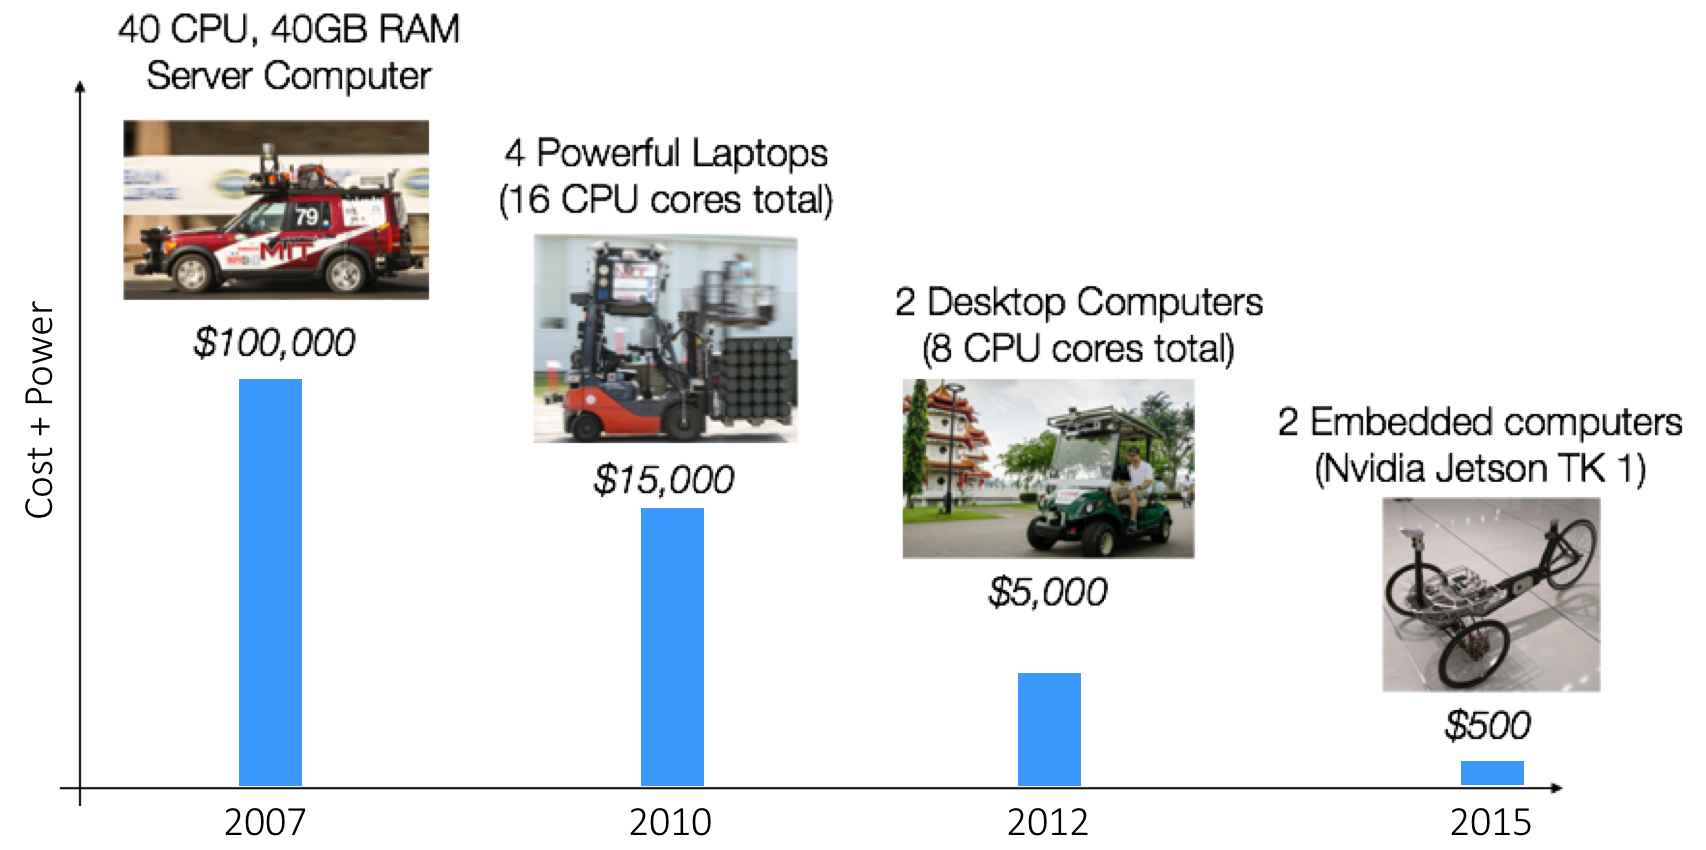
\includegraphics[width=\linewidth]{figs/01/computerCost2}
	\caption{The cost and the computational power required for self-driving cars has been greatly reduced during the last decade.}
\end{figure}

On the other side, throughout the last decade there has been an incredible decrease in the cost of computation time and in the size and power to process the data coming from the sensors. This point is critical in order to incorporate compact and affordable autonomy packages in current cars.

\begin{figure}[h]
	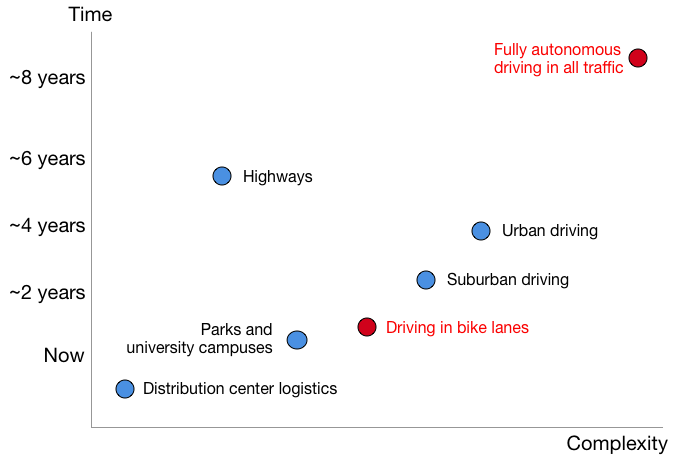
\includegraphics[width=\linewidth]{figs/01/autonomy_speed2}
	\caption{Challenges of self-driving vehicles based on the time of deployment and the complexity of the task.}
\end{figure}

However, achieving a level 5 of autonomy (based on SAE International Standard J3016\cite{SAEj3016}) will require years of development, due to the complexity of the task. Driving in bike lanes, on the contrary, makes up a straightforward challenge, basically because the road conditions and the sensors required for this task are not that demanding. The use of less and more affordable sensors will allow the deployment of intelligent three --or two in the future-- wheeler vehicles through bike lanes.

\subsection{Sharing Economy}

During the last couple of years, the sharing economy has disturbed the traditional way of moving in cities. Companies as \textit{Uber, Lift, BlaBlaCar, GetAround, Turo, Zipcar} and many others have offered a new way of commuting in urban areas. In this new paradigm, the technology has arrived to some countries without a proper regulation, which has caused complaints and protests from conventional transit services.
Other sectors, as housing (\textit{Airbnb}), goods (\textit{Wallapop}), food (\textit{LeftoverSwap}), sports equipment rentals (\textit{Spinlister}), and tourism (\textit{Vayable}) have also seen the irruption of this new way of economy.

More and more cities around the globe have adopted so called bike-sharing systems, which enable citizens and visitors to pick up bicycles at some point in the city, use them and leave them at another point in exchange for a small fee.

\newpage

\begin{figure}[t]
	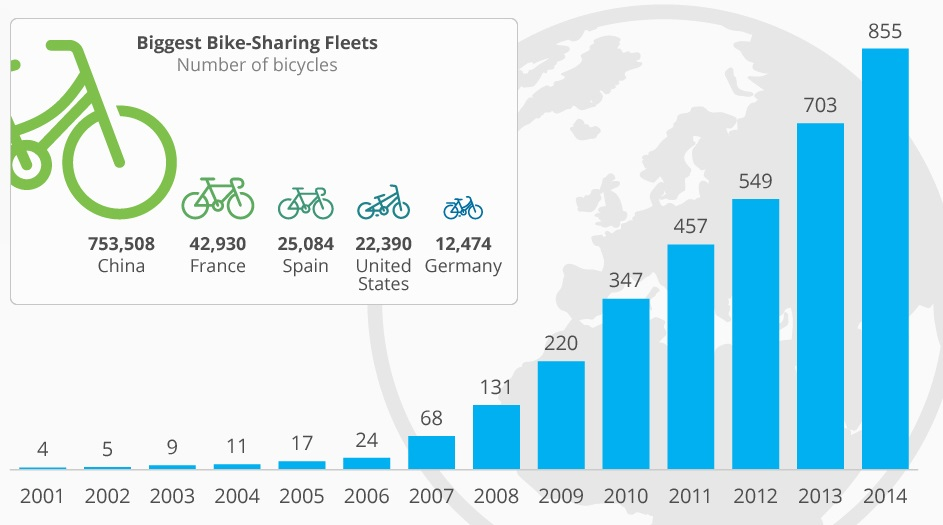
\includegraphics[width=\linewidth]{figs/01/Bike_Sharing_Systems_Worldwide}
	\caption{Number of cities worldwide that offer bike-sharing services. Source: \url{https://www.statista.com/chart/3325/bike-sharing-systems-worldwide/}}
\end{figure}




\subsection{Car-less Cities}

The ultimate policy will be to get rid of the vehicles in the city centers, as multiple cities have already announced.\cite{carFree} These can be seem as very radical strategies in transport policies, but the congestion and the pollution big cities are suffering at this moment exhibit much more issues and harm.

Therefore, is it possible to leverage electrification, autonomy and the shared economy to help fulfill this vision while ensuring a convenient flow of people and goods across the city?

%\newpage
\section{Persuasive Electric Vehicle}
Changing Places group\cite{cp} at MIT Media Lab\cite{ml} believes in the progressive fading of conventional cars from urban areas. The group's vision recalls on Kent Larson's\cite{kll} ideas, who affirms that the introduction of autonomous, electric and shared vehicles will hugely impact the cities of the future: Different streets layout, no more parking problems, less necessary vehicles and the overall result will be that the citizens will take the streets back from the cars. 

Furthermore, most trips in the city are one-person, low-speed, short distance. It does not make any sense to put one person in a 1800 kilograms vehicle to move across a city only a couple of kilometers. It was in front of this situation when the Changing Places group designed an ultra-lightweight one-person, three-wheel vehicle that is bike-like, not car-like.

\begin{marginfigure}
	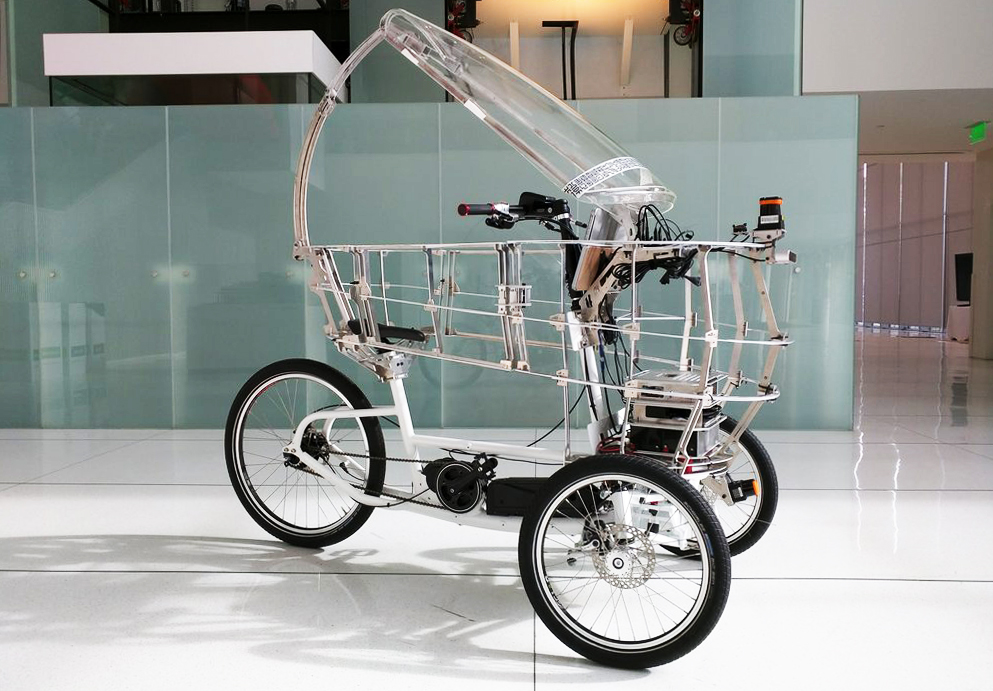
\includegraphics[width=\linewidth]{figs/01/pev_4}
	\caption{Persuasive Electric Vehicle (september 2016)}
\end{marginfigure}

\newpage
The \textbf{Persuasive Electric Vehicle}\cite{pev} (PEV) is an agile, on-demand, shared and functionally-hybrid tricycle with an expected contribution of 60\% emissions reduction and 30\% vehicle-distance reduction. The PEV is thought to constitute a new and indispensable category of vehicles in the emerging constellation of mobility systems. 

The PEV takes advantage of existing bicycle lanes, provides energy-efficient mobility, and addresses sedentary lifestyles. Designed with a cover to protect from the rain and the option for electric assist, PEV makes biking compelling for various demographics. 

Various \textbf{persuasive interventions} are displayed through user interaction with smartphones to facilitate pedaling behavior. Influential strategies are designed for both the interior and exterior of PEV. For example, an interior display shows how many previous riders have actually pedaled while riding a particular PEV. The exterior of the PEV changes color depending on whether a rider actually pedals or not.

\begin{figure}
	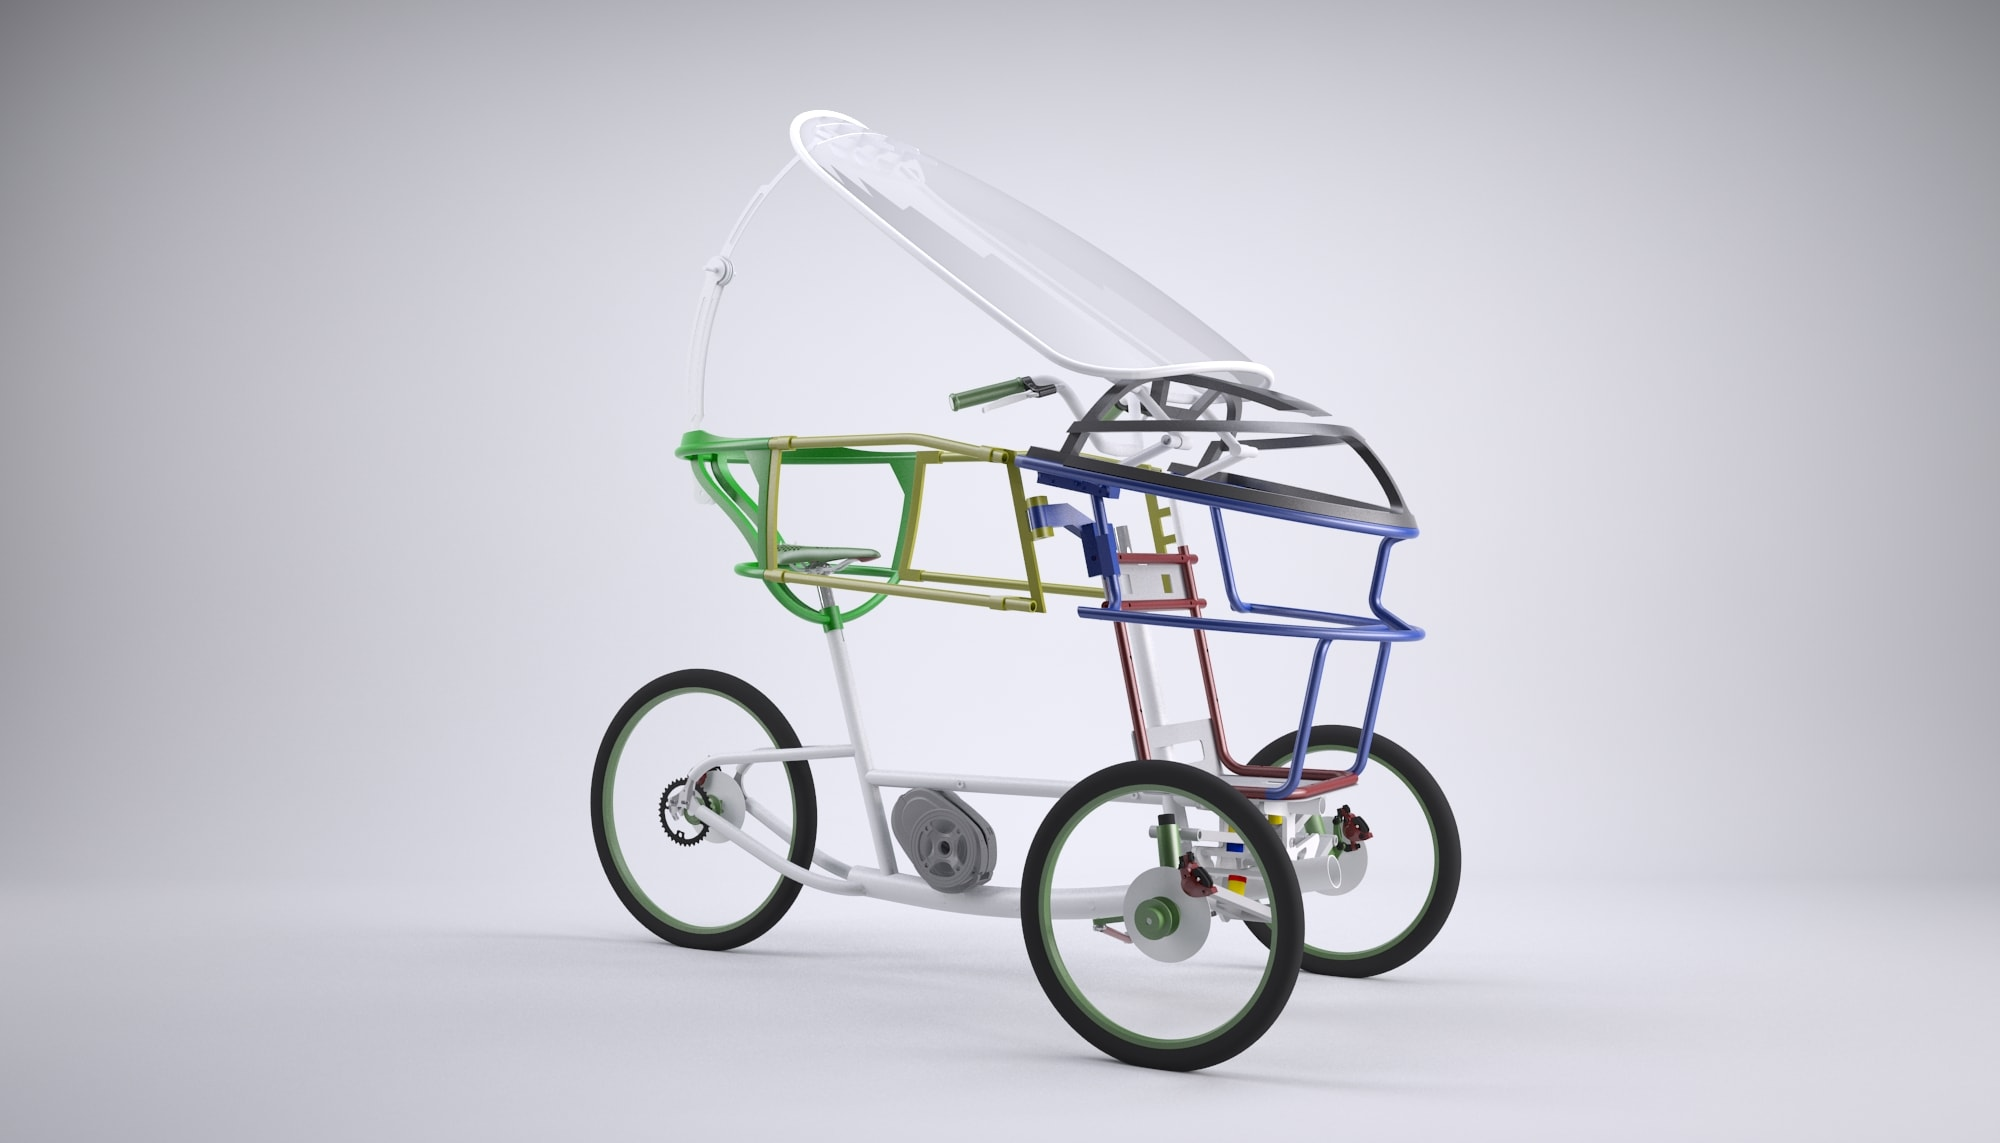
\includegraphics[width=\linewidth]{figs/01/pev_5}
	\caption{Persuasive Electric Vehicle render model}
\end{figure}

With a fabric exterior shield, a foldable canopy, and a 250-watt assist motor, the autonomous tricycle is "persuasive" in that it is designed to "encourage positive modal shifts in mobility behavior in cities." It has a top speed of 12 miles per hour, limited by the US regulation. It can be adapted for a human rider or for package transport, and it has the sensors and intelligence to operate autonomously.
 
\newpage
\subsection{Functionality}

-- \textbf{In transportation of goods} mode, the PEV will cover delivery on what is known as "the last urban mile". The PEV will be used as an autonomous courier service taking advantage of its attributes --small and maneuverable-- to efficiently service congested city areas even in cases of traffic cuts. 

\begin{marginfigure}
	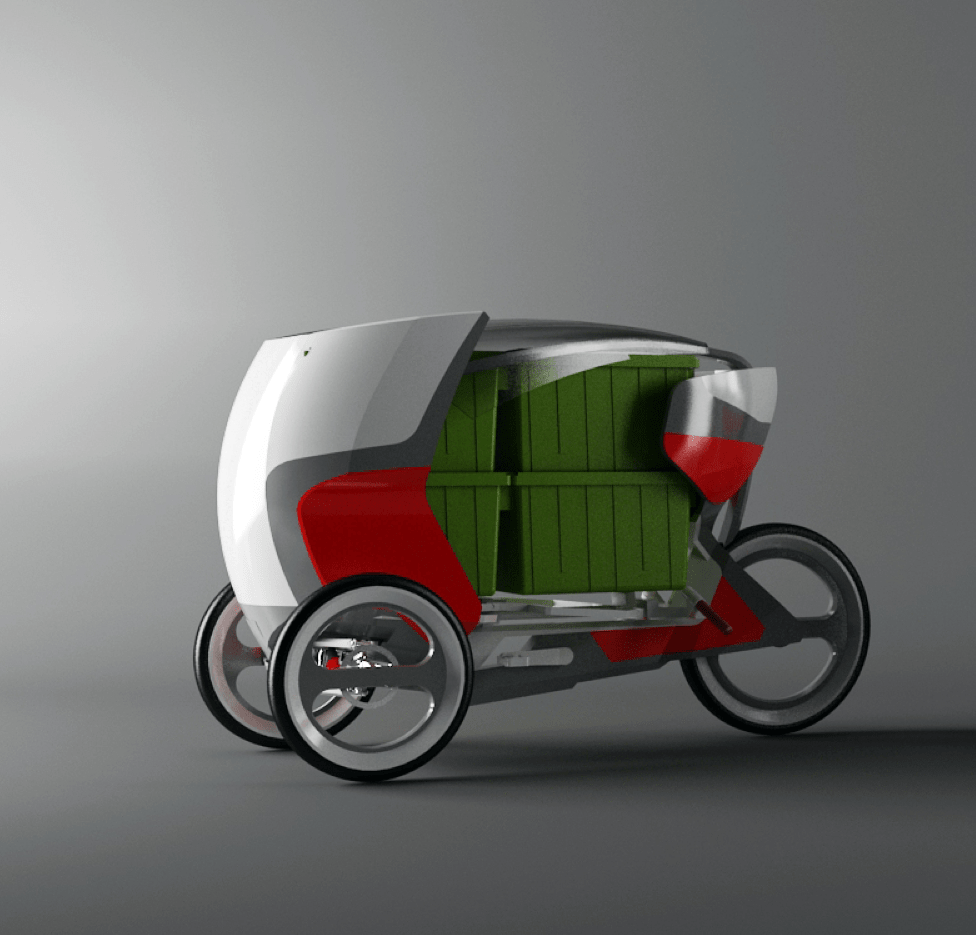
\includegraphics[width=\linewidth]{figs/01/folded}
	\caption{Logistics Mode PEV}
\end{marginfigure}

It could become a pervasive mode for urban package delivery, moving easily through crowded streets and reducing congestion and carbon emissions from gas-powered delivery vehicles.

-- \textbf{In passenger transport} mode, the PEV would function as a bicycle providing more safety and comfort thanks to its structural design, which offers more protection than conventional bikes, as well as its electrical assistance system, easing effort while pedaling.

Opposed to most shared bike systems, the PEV would "redistribute itself". Traveling autonomously from the drop-off point of one passenger to its next user's location, thus solving the problem of shortages and oversupply of bikes at different times in different locations. 

\begin{marginfigure}
	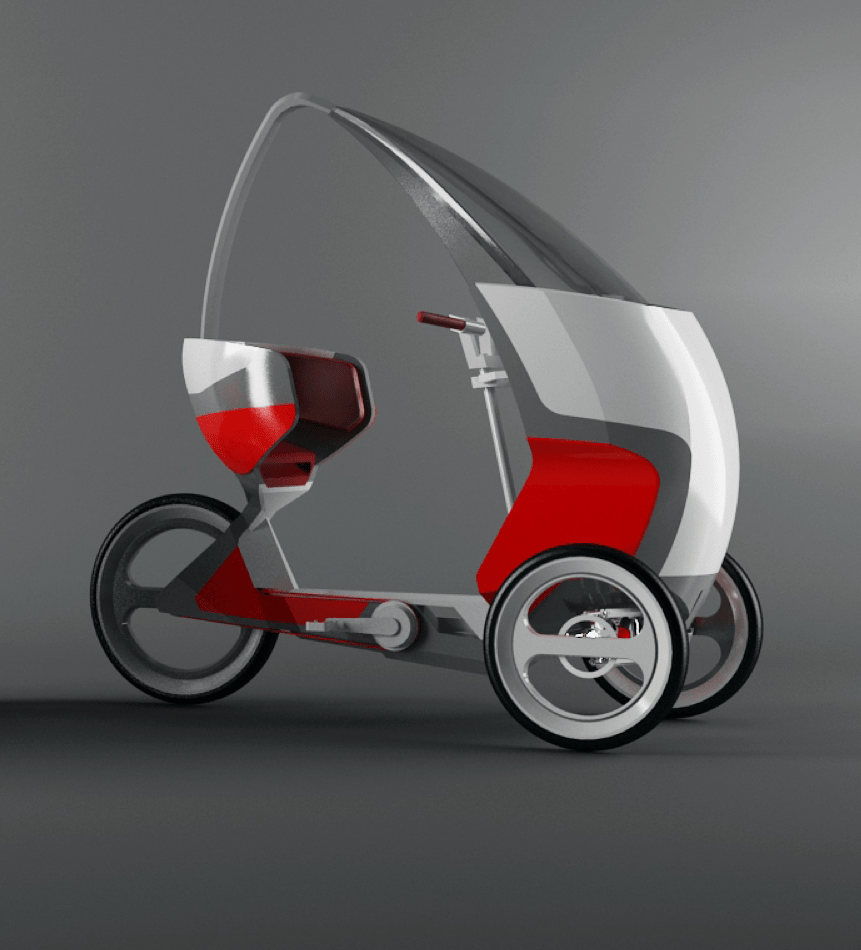
\includegraphics[width=\linewidth]{figs/01/unfolded}
	\caption{Passenger Mode PEV}
\end{marginfigure}

As for the \textbf{persuasive element}, studies show that those using ride sharing programs were already walking or riding their bikes more than others. Since the PEV is meant to expand the market for sustainable transportation, its focus is to give automobile drivers a reason to switch over-which is, a little exercise. By pedaling, riders generate energy that is stored up and used when needed by the motor. Passengers could choose to take care of their bodies, cities, and environment at the same time.

\subsection{Concluding Remarks}

The PEV is one of the upcoming new technological innovations that are set to change the way people commute in urban areas. Concerns over pollution and congestion of cities due to the increasing numbers of vehicles have seen man engage in inventions to improve their communities. Automobiles contribute largely to pollution; the development and use of the PEV would introduce an ecological mode of transportation. The elderly will also have reliable means of movement, which in turn encourage exercise and fitness.

\newpage
\section{Motivation}

The development of a new concept of intelligent vehicle opens the door to new research projects, in a \textbf{wide range of fields}. Computer vision, vehicle fleet simulations, persuasive technologies, mechanical design...are only few examples. Due to the open research opportunities, there is the necessity to understand in first place what people feel about the vehicle, from a user point of view. The conclusions of this analysis will narrow down the spectrum to this project's topic.

\subsection{Amazon Products Reviews}


A good way of understand the feelings of the people is to ask previous users about similar products. In this case, the most similar product was found in \textbf{adult tricycles}. The PEV's user demographics coincides with these vehicles users. Nowadays, one of the best databases of available user information can be found in Amazon\cite{Amazon}.

However, this information is not easily accessible. While it is true that Amazon used to provide access to product reviews through their Product Advertising API to developers and sellers, the company discontinued that on November 2010, preventing customers from displaying Amazon reviews about their products, embedded in their websites. As of now, Amazon only returns a link to the review.

Therefore, getting this data requires other methods. In this project, the dataset of Amazon reviews was downloaded using a \textbf{web crawler on the HTML} pages\cite{perl}. Given a first level domain ("com") and the list of IDs of Amazon products, this Perl script automatically downloads, from the Amazon server that is dedicated to that domain, all and only the HTML pages that contain the reviews about that products.

Another Perl script extracts all the reviews contained in the downloaded HTML files, outputting for each review a record with the following information:

\begin{itemize}
	\begin{itemize} \itemsep -15pt
		\item A counter of the extracted reviews
		\item Date of the review in \textsc{YYYY/MM/DD} format
		\item ID of the reviewed product
		\item Star rating assigned by the reviewer
		\item Count of "yes" helpfulness votes
		\item Count of total helpfulness votes ("yes"+"no")
		\begin{marginfigure}
			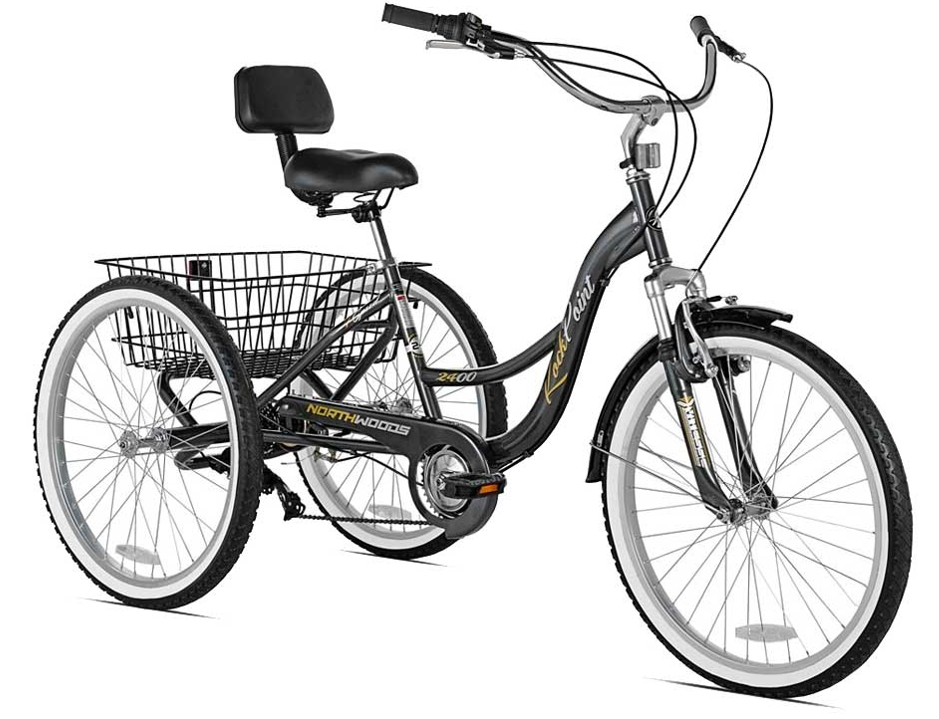
\includegraphics[width=1.2\linewidth]{figs/01/prodExample}
			\caption{One of the selected Amazon products}
			\label{prodExample}
		\end{marginfigure}
		\item Date of the review
		\item ID of the author of the review
		\item Title of the review
		\item Content of the review
	\end{itemize}
\end{itemize}

The selected products are really similar, with color, some components and accessories as main distinctions. The Figure \ref{prodExample} illustrates an example of one of the selected products, and more information has been included in Table \ref{productInfo}.

\begin{table*}[h!]
%\centering
\fontfamily{ppl}\selectfont
\label{productInfo}
\\[10pt]
\begin{tabular}{llc}
	\hline
	\textbf{Product ID} & \textbf{Product Description}  & \textbf{No. Reviews} \\
	\hline
	{B000IORU06} & Schwinn Meridian Adult 26-Inch 3-Wheel Bike           & 401\\
	{B000Z89JFO} & Kent Adult Westport Folding Tricycle                  & 157\\
	{B003F1WMZC} & Worksman Port-o-Trike Three Speed Adult Tricycle      & 42 \\
	{B00AWNI22I} & Schwinn Meridian Tricycle (26-Inch Wheels)      		 & 11 \\
	{B00FXMIUPW} & Mantis Adult's Tri-Rad Folding Trike					 & 2  \\
	{B00KDJC5UQ} & Komodo Cycling 24, 6-speed Adult Tricycle             & 2  \\
	{B00G3N5MZ6} & Torker 24 x 20 TriStar 2.1 Adult Trike 3 Speed        & 1  \\
	\hline
\end{tabular}
\\[15pt]
\caption{Detailed information about the analyzed Amazon products}
\end{table*}


Overall, over 670 reviews were extracted, being the Schwinn model the product with most of the reviews. Obtaining this information required a great deal of time, since Amazon does not like to have its web-page scraped, and the access gets banned, so a delay has to be introduced. This sleep delay starts with 5 seconds and increases over time, making really tedious to get the review data.

An alternative to this method would have been to use an already existing dataset. This option was studied, but it was not able to find any of the scoped products on the dataset, due to the available period of data (up to July 2014).

Having extracted the data, different approaches were implemented in parallel to understand the overall opinion of the users. In this way, it has to be pointed out that the review comments were predominantly too brief and that hardly expressed valuable ideas or details about the product. The majority of the users just valued the product from a very general perspective. Even with more than 670 reviews, the quality of the reviews could mislead the data analysis.

In the next section three analysis are explained, with their corresponding scripts included in the Appendices. I would encourage the reader to review the scripts after the following section, since the scripts include much more information and details while here brief explanations and the main conclusions are going to be explained.

%\newpage
\subsubsection{\textbf{Sentiment Prediction Analysis}}

\begin{marginfigure}
	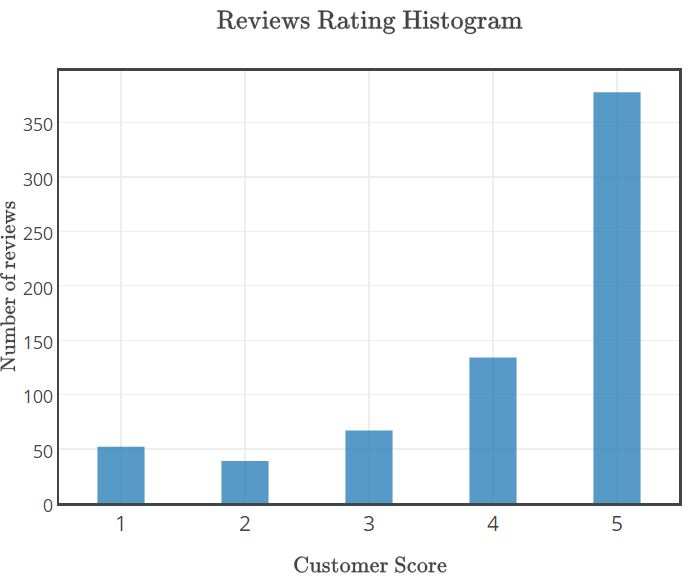
\includegraphics[width=1.3\linewidth]{figs/01/review_score}
	\caption{Reviews Rating Histogram}
	\label{starDistribution}
\end{marginfigure}

The purpose of this analysis was to investigate the positive and negative attitudes towards the selected products. Sentiment analysis attempts to determine which features of text are indicative of it's context (positive, negative, objective, subjective, etc.) and build systems to take advantage of these features.

Generally speaking, a satisfied customer will give 5 stars to the product, whereas few users will give poor evaluations (only if something really bad happened). This behavior is visualized in Figure \ref{starDistribution}, where the 5-star evaluation prevails.

This skewed distribution makes difficult to do a sentiment analysis based on the star-evaluation of the user. That is why the focus was not on the Score, but only in the positive/negative sentiment of the recommendation. Out of this analysis, the most positive and negative words are obtained:

\begin{figure*}
	\caption{Top 10 positive \& negative expressions and their score}
	\minipage{0.5\textwidth}%
	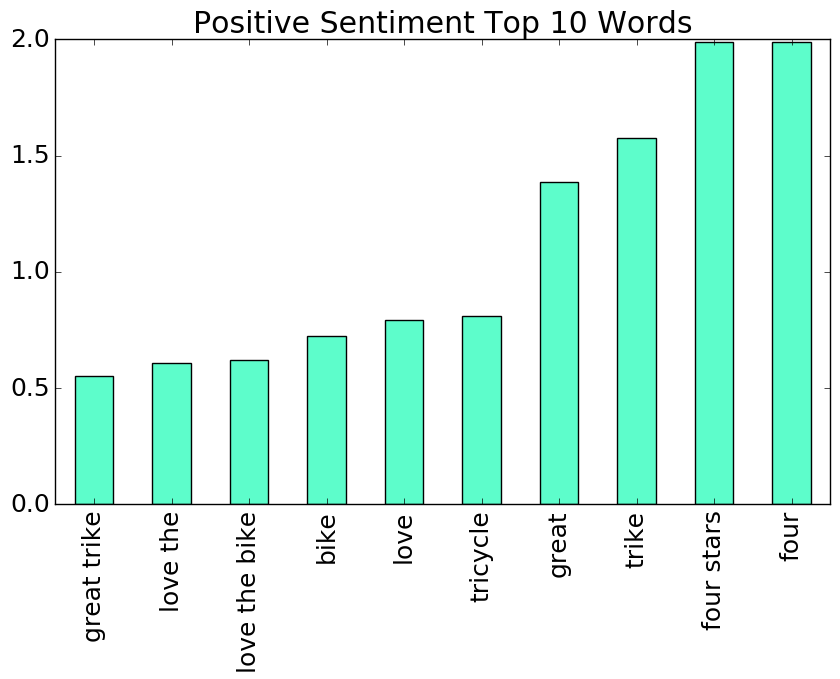
\includegraphics[width=1\linewidth]{pdf/Predicting_Sentiment_and_Helpfulness/Predicting_Sentiment_and_Helpfulness_files/Predicting_Sentiment_and_Helpfulness_13_2}
	\endminipage
	\minipage{0.5\textwidth}%
	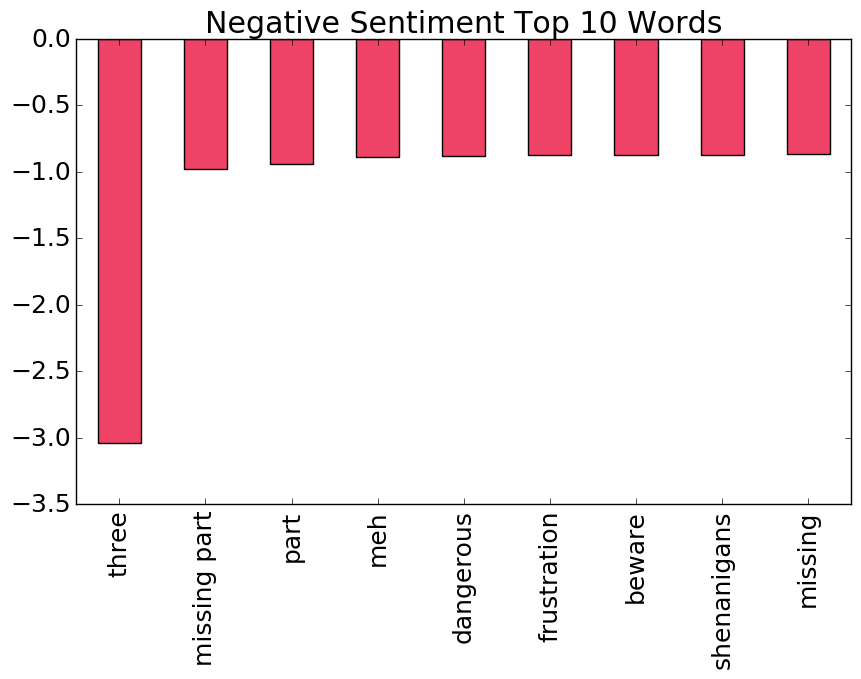
\includegraphics[width=1\linewidth]{pdf/Predicting_Sentiment_and_Helpfulness/Predicting_Sentiment_and_Helpfulness_files/Predicting_Sentiment_and_Helpfulness_13_1}
	\endminipage
	\\[6pt]
\end{figure*}

On the positive side, not much can be concluded, due to the lack on details. Customers that like the trike simply say it is a great product ("\textit{Four Stars}","\textit{Great},"\textit{Love}"), without saying why. This is totally opposite to the negative side, where much clear expressions appear.

\begin{table}[h!]
\centering
\label{most}
\begin{tabular}{cc}

	\begin{tabular}{c}
		\hline
		\textbf{Most Positive}\\
		\hline
		Four Stars\\
		Trike\\
		Great\\
		Tricycle\\
		Love \\
		Love the Bike\\
		Great Bike\\
		\hline
	\end{tabular}
	&
	\begin{tabular}{c}
		\hline
		\textbf{Most Negative} \\
		\hline
		Three\\
		Missing Part	\\
		Meh \\
		Dangerous\\
		Frustration    \\
		Beware		\\
		Shenanigans    \\
		\hline
	\end{tabular}
\end{tabular}
\\[10pt]
\caption{Selected relevant positive and negative expressions extracted from the sentiment analysis}
\end{table}

The main worries of the users are the missing parts from the trike and the danger or riskiness of the trike. The feelings of the user towards the product are summarized in "Meh" and "Frustration", both probably related to the assembly of the product. It also seems that the trike is dangerous to ride and that users should be aware of possible falls. For this project interest, one of these products weaknesses is starting to show up.

More information and the implementation of this program can be found in the
\hyperref[Predicting_Sentiment_and_Helpfulness]{\textcolor{blue}{Predicting Sentiment}} script on the Appendices.

\subsubsection{\textbf{Topic Modeling - LDA}}

Another way of analyzing the user data is to follow the topic modeling approach. By taking inferred topics and analyzing the sentiment of their corresponding documents (reviews) what customers are saying (or feeling) can be found. Examples from other authors\cite{bhatt2015amazon}\cite{chakankarsentiment}\cite{Mukherjee2012}\cite{rain2013sentiment}.

Latent Dirichlet Allocation (LDA) is the technique used to extract topics from Amazon reviews. It is assumed that there is some number of topics (manually chosen, 10 topics in this case), each topic having associated probability distribution over words and each document has its own probability distribution over topics. 

First, it scopes out a bunch of different \textbf{documents}, making note of the \textbf{words} in each of them. Crucially, it does not know the \textbf{topics} of each document, neither the different topics of each word.

Therefore, it picks some number of topics to learn, and starts by making a guess as to why each word belongs to each document. Of course, the random guesses are very likely to be incorrect, but there is a way to improve them, known as Gibbs sampling:
\begin{itemize}[noitemsep]
\begin{itemize} [topsep=6pt]
\item Go through each word $w$ in document $d$
\item For each topic $k$, computes two things: 
	\begin{itemize}
	\item p($k$|$d$) = the proportion of words in document $d$ that are currently assigned to topic $k$
	\item p($w$|$k$) = the proportion of assignments to topic $k$ over all documents that come from this word $w$. 
	\end{itemize}
\item Reassign word $w$ a new topic, where we choose topic $k$ with probability p($k$|$d$) * p($w$|$k$). According to the generative model, this is essentially the probability that topic $k$ generated word $w$.
\end{itemize}
\end{itemize}

\marginnote{
Specific Notation: \\
$\beta_{K}$ Topics\\
$\theta_{d}$ Topic proportions for document $d$ \\
$z_{d,n}$ Topic assignment for word $n$ in document $d$ \\
$w_{d}$ Observed words from document $d$ \\
$\eta,\alpha$, Dirichlet parameters \\
}
Finally it takes into account the distribution of each topic in each document (with the parameters $\alpha$ and $\eta,$ leading to:

\[p(\beta,\theta,z,w)=
\prod_{i=1}^K p(\beta_{i}) \prod_{d=1}^D p(\theta_{d}) \prod_{n=1}^N p(z_{d,n}|\theta_{d}) p(w_{d,n}|\beta_{1:K},z_{d,n})\]
 
 \begin{figure}
	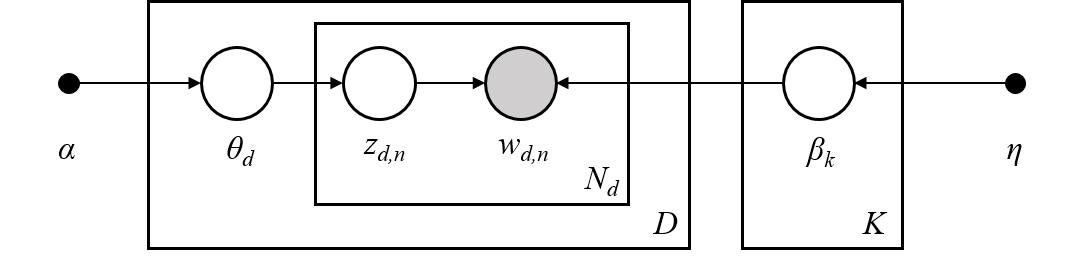
\includegraphics[width=1\linewidth]{figs/01/LDA}
	\caption{LDA graphical model. Boxes represent replicates. Outer box $D$ are documents, while inner box $N_d$ represents the repeated choice of words within the document}
	\label{LDA_graph}
\end{figure}

\newpage
Summing up, Gibbs sampling\cite{mcauley2015} basically takes some initial values of parameters and iteratively replaces those values conditioned on its neighbors (Figure \ref{LDA_graph}). Every word in all the text reviews is assigned a topic at random, iterating through each word, weights are constructed for each topic that depend on the current distribution of words and topics in the document, and we iterate through this entire process until it reaches a convergence.

All the reviews were converted to a bag of words and stop words removed. After the training of the model, a query was made passing a selected string to the model: "issues".

\begin{figure*}
	\caption{Results from the query to the LDA model: words from the most and less related topics}
	\minipage{0.5\textwidth}%
	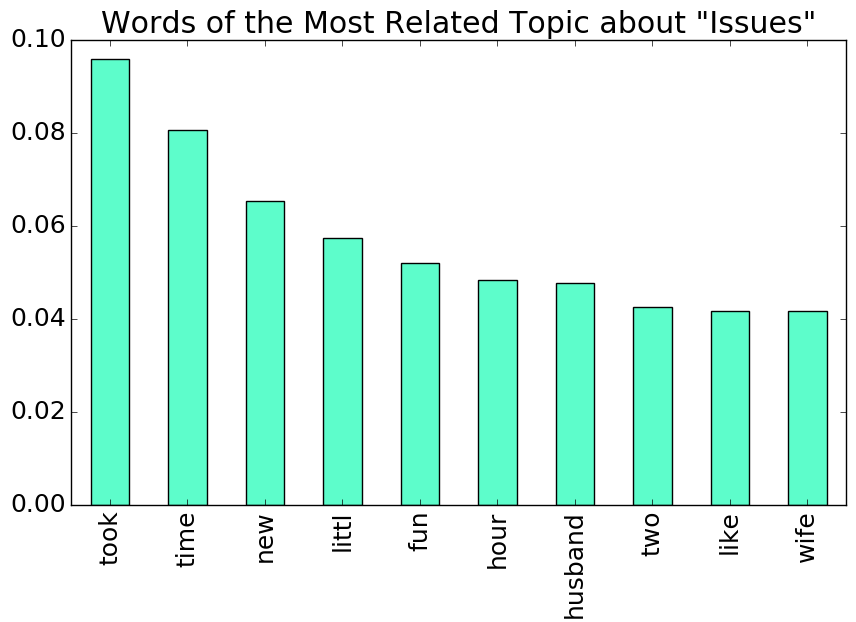
\includegraphics[width=1\linewidth]{pdf/Topic/Topic_Modeling_Amazon_Reviews_files/Topic_Modeling_Amazon_Reviews2_42_2}
	\endminipage
	\minipage{0.5\textwidth}%
	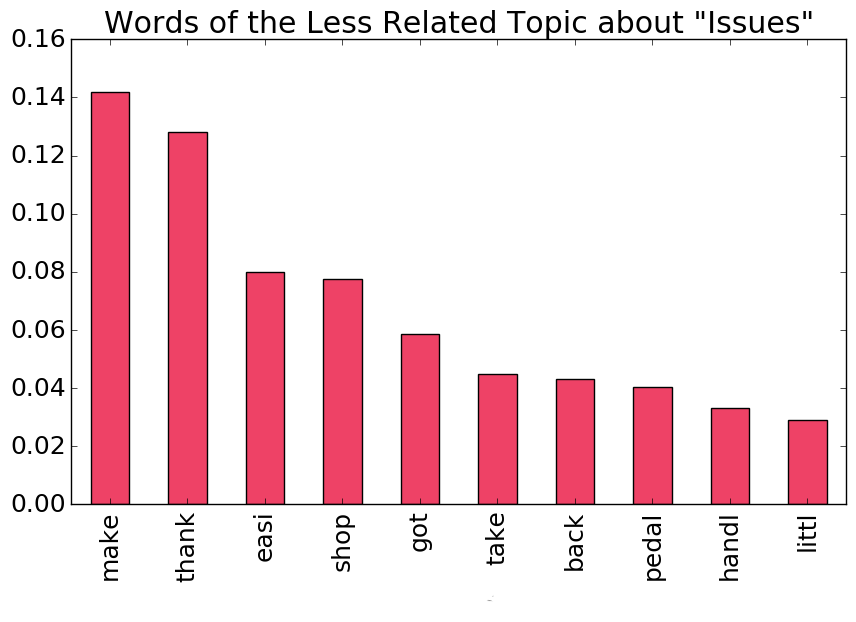
\includegraphics[width=1\linewidth]{pdf/Topic/Topic_Modeling_Amazon_Reviews_files/Topic_Modeling_Amazon_Reviews2_42_1}
	\endminipage
	\\[6pt]
\end{figure*}

The most related topic (0.66 correlation) talks about assembly issues, with words like "\textit{took}", "\textit{time}", "\textit{little}", "\textit{fun}", "\textit{husband}", "textit(wife)", whereas the less related topic (0.03 correlation)  contains ("\textit{make}", "\textit{thank}", "\textit{easy}", "\textit{shop}", "\textit{bak}"), which has little to do with any issues or problems. In fact, it seems this topic has not a clear meaning behind.
Fortunately, both topics do no share words, leading to the conclusion that these topics are far apart, and that are related to different aspects of the products.

As a conclusion to this analysis, the assembly of the bike (that comes in parts) supposes main problem to the users, an issue that will be out of the scope of this project. 

Overall, the results are not clear enough to to make an inference about their cause or origin. As the reader can notice, this analysis was not that successful, because the results could be interpreted in various different ways. Having only unigrams does not help to the interpretation of the results. That is why another way was approached, by means of keyword extraction and the wordcloud creation.

More information and the implementation of this program can be found in the
\hyperref[Topic_Modeling_Amazon_Reviews]{\textcolor{blue}{Topic Modeling}} script on the Appendices.

\subsubsection{\textbf{Wordcloud Creation}}

The Rapid Automatic Keyword Extraction (RAKE)\cite{rake} algorithm was implemented to easily extract keywords from the reviews, by identifying runs of non-stopwords and then scoring these phrases across the document. It requires no training, the only input is a list of stop words for a given language, and a tokenizer that splits the text into sentences and sentences into words.
 


A typical keyword extraction algorithm has three main components:
\begin{enumerate}\itemsep -10pt
	\item \textbf{Candidate selection}: extract all possible words, phrases, terms or concepts that can potentially be keywords.
	\item \textbf{Properties calculation}: For each candidate, calculate properties that indicate that it may be a keyword.
	\item \textbf{Scoring and selecting keywords}: All candidates can be scored by either combining the properties into a formula, or using a machine learning technique to determine probability of a candidate being a keyword. A score or probability threshold, or a limit on the number of keywords is then used to select the final set of keywords.
\end{enumerate}
	Finally, parameters such as the minimum frequency of a candidate, its minimum and maximum length in the words, or the stemmer used to normalize the candidates help tweak the algorithm's performance to a specific dataset.
	
\begin{marginfigure}
	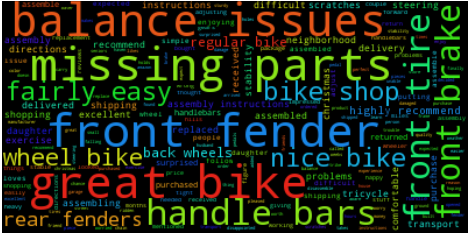
\includegraphics[width=1.2\linewidth]{pdf/Amazon/Amazon_clean_files/Amazon_clean_4_1}
	\caption{Unformated wordcloud of extracted keywords}
	\label{wordcloud1}
\end{marginfigure}
	
	In the Figure \ref{wordcloud1} there is the first version of the extracted wordcloud, without any format, and Figure \ref{wordcloud2} is the result after the formatting. The shape of the wordcloud was taken from one of the Amazon products, to simulate the form of a tricycle. More information and the implementation of this program can be found in the \hyperref[Amazon]{\textcolor{blue}{Wordcloud Creation}} script on the Appendices.
	
	From the wordcloud there were positive terms, as "\textit{great bike}", "\textit{front fender}", "\textit{fairly easy}","\textit{highly recommend}". Focusing on the negative features, some interesting terms appeared: "\textit{missing parts}", "\textit{rear fenders}", "\textit{bike shop}","\textit{balance issues}". Out of curiosity, these trikes do not have rear fenders but do have one in the front, leading to the users complains.

As a mechanical engineer, the term "\textit{balance issues}" was the one that attracted my attention. How can a three wheeler bike have balance issues? It is in fact intrinsically more stable than a bike, for sure. However, searching manually through some reviews, I noticed that the origin of this term was in some people complaining about falling when taking a curve, or one of the rear wheels lifting the ground. All these experiences made the users feel insecure when riding the trike. What could be done to avoid this problem?

\begin{figure}[t]
	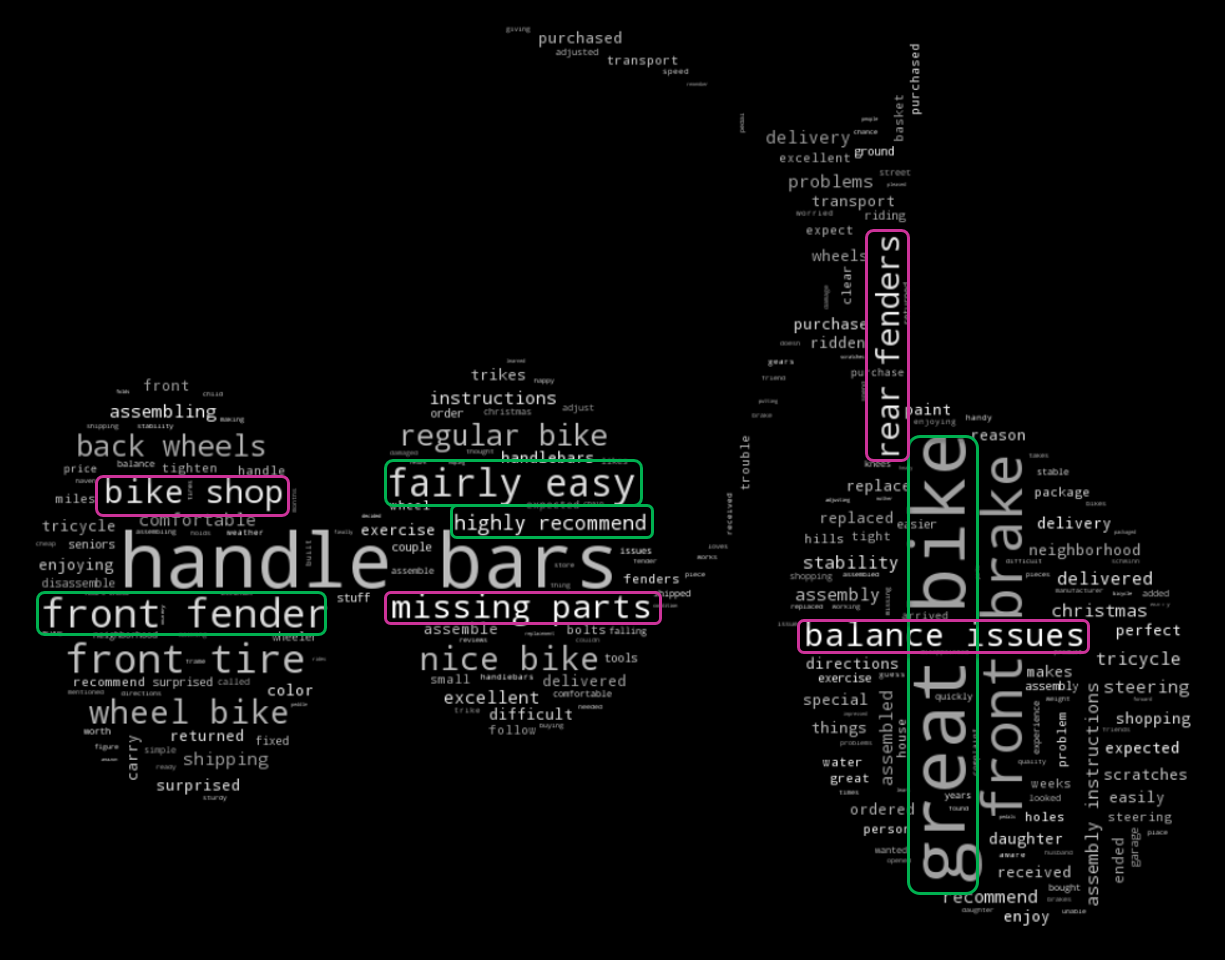
\includegraphics[width=1\linewidth]{pdf/Amazon/Amazon_clean_files/Amazon_clean_6_1}
	\caption{Formated wordcloud of extracted keywords}
	\label{wordcloud2}
	\\[-1cm]
\end{figure}

\section{Narrow Track Vehicles}

Balance or stability issues only appear when the user goes into a curve, otherwise the three wheels always support the trike in stable position. Let us analyze these type of vehicles in terms of the stability.

The PEV can be classified as a narrow track vehicle and, as it operates in normal driving conditions, it needs to be relatively tall to assure visibility. In Figure \ref{pevDim} the bounding box dimensions are represented. A tall narrow vehicle is characterized by a high centre of gravity to track width ratio, which makes vehicle \textbf{roll stability} an issue\cite{Saeedi}\cite{festini2011urban}.

When the track width of a vehicle is narrowed, there is an increasing in the the ratio of the center of gravity height with respect to the track width. This particular geometric property poses \textbf{stability problems for these types of vehicles while cornering}. Hence, such a narrow vehicle needs to be equipped with an inherent tilting mechanism that enables the vehicle to \textbf{tilt into turns while cornering}\cite{nurse2015tilting}. 

The added tilt degree of freedom should not require any stabilizing input from the driver. This brings about the need for an active control system that ensures the tilt stability (appropriate leaning during cornering) without affecting the handling of the vehicle.

\begin{figure}[t]
	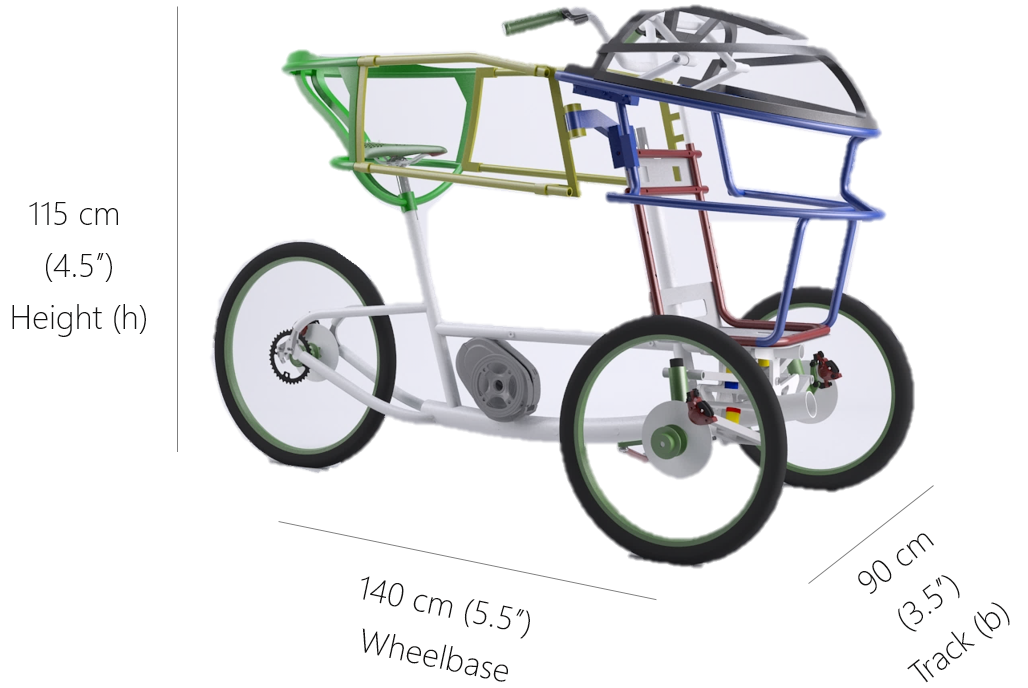
\includegraphics[width=1.0\linewidth]{figs/01/pev_6}
	\caption{PEV bounding box dimensions}
	\label{pevDim}
\end{figure}

Therefore, if such a vehicle is to negotiate curves through out its operating speed range, it needs to have a \textbf{capacity to tilt into the curve} like most two-wheeled vehicles. Consequently, an inherent tilting capability is required. 

This \textbf{tilting mechanism} should not require any special skills from the driver. The driver should be able to drive about as he/she would a regular four-wheeled vehicle. This, in turn, brings about a need for an \textbf{active tilt control system} that controls the tilting mechanism and ensures the stability of the vehicle and safety of the driver.

%\begin{marginfigure}
%	\centering
%	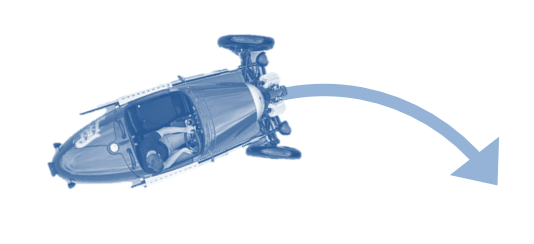
\includegraphics[width=1.15\linewidth]{figs/01/turn}
%	\caption{Right turn scenario for stability}
%	\label{turn}
%\end{marginfigure}

\subsection{Stability}

\marginnote{\\
$h_{g}$ Height of the center of gravity\\
$b$ Wheelbase width\\
$R_{l}, R_r$ Left and right wheel reactions\\
$F_y$ Lateral force\\
$T_{r}$ Moment due to the reactions $R_{l}, R_r$\\
$T_{f}$ Moment due to lateral force $F_y$\\
$m$ Mass of the vehicle\\
$g$ Earth gravity acceleration\\
}

Narrow vehicles that do not lean are unstable when they corner too hard. A simple statics calculation can illustrate this fact (Figure \ref{balance}).  

As the vehicle accelerates, for example, in a turn to the right, due to increasing lateral force $F_y$, the reaction in the right wheel $R_r$ approaches zero while the reaction in the left one $R_{l}$ approaches the weight force $mg$. 

At the balance limit, \[T_{r} = \frac{bmg}{2}\] and \[T_{f} = 2hF_{y}\]Overturning occurs if $T_{r} < T_{f}$, or similarly, the wheelbase is limited to \[b < \frac{4hF_{y}}{mg}\]By introducing tilt control, the \textbf{center of gravity is shifted} so that $R_r$ never reduces to zero. 

\begin{marginfigure}[-1cm]
	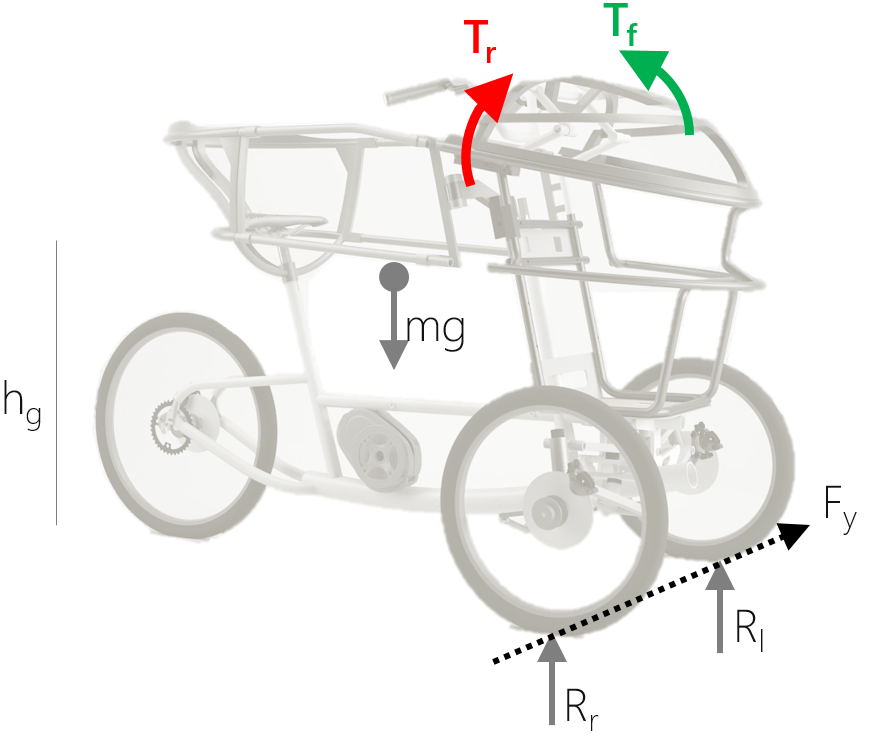
\includegraphics[width=1.3\linewidth]{figs/01/pev_7}
	\caption{Force schematic in a right turn scenario}
	\label{balance}
\end{marginfigure}

\newpage
\section{Research Objectives}

\begin{marginfigure}
	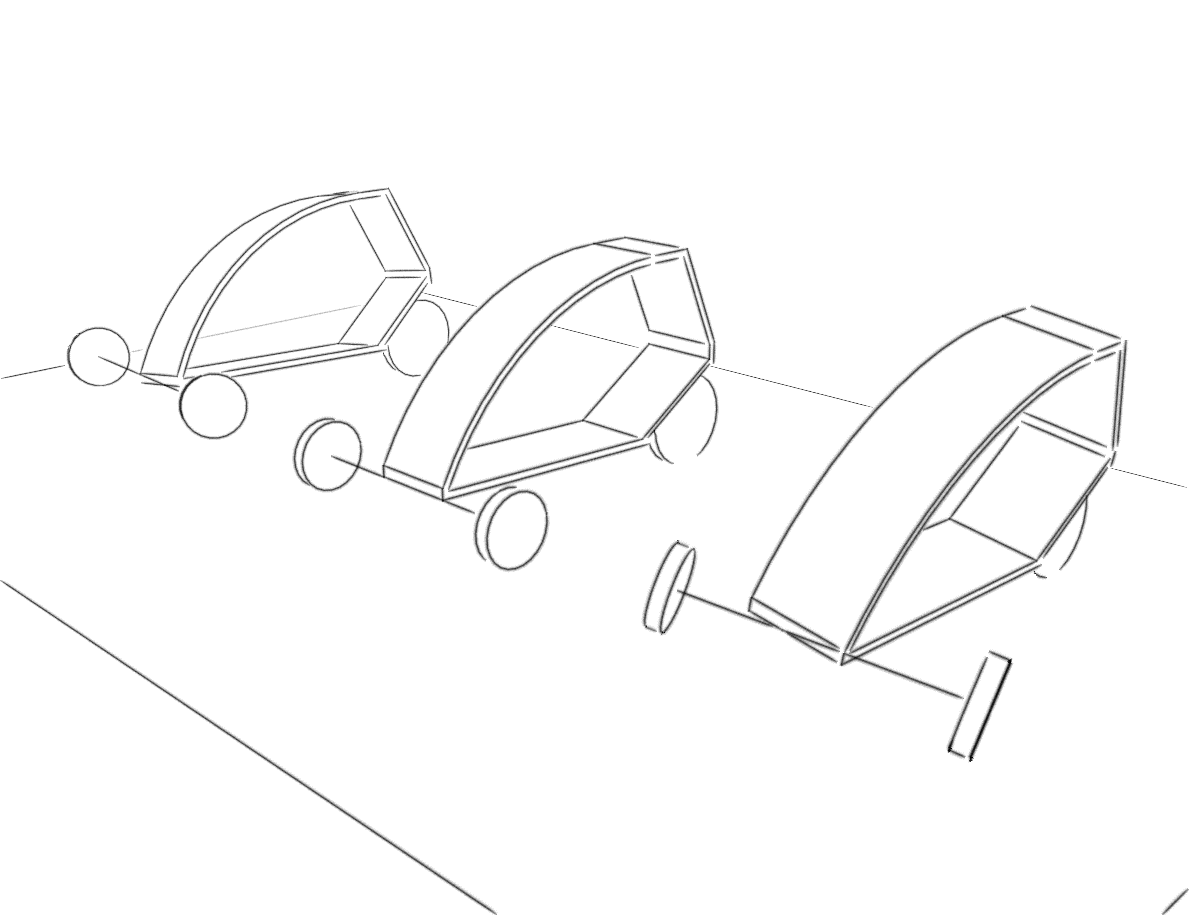
\includegraphics[width=1.3\linewidth]{figs/01/tilting_sketch}
	\caption{Simple first sketches of a tilting PEV}
\end{marginfigure}

This project is going to consist on the \textbf{design and fabrication of a three wheeler vehicle with an active tilting system}. The aim of the work presented here is summarized as follows:

\begin{itemize}\itemsep -8pt
	\begin{itemize}
	\item  The main objective was to \textit{design and fabricate a three-wheeled tilting vehicle} and to \textit{implement a roll control system}. In this way, due to the size, weight and cost limitations of a lightweight vehicle like PEV, it was critical to constrain the size of the motors and the feasible mechanical components.
	
	\item The first aim was to \textit{review the current developments} in vehicle modeling, roll control and tire modeling. Understanding the previous work in this field is fundamental to know the limitations and problems of the applied techniques. 
	
	\item The second aim was to implement and investigate models and methods to quantify uncertainties in the vehicle system such as the kinematics and environmental factors. These factors had a direct effect on the experimental results of road tests as well as the vehicle modeling and simulation. 
	
	\item The final aim was to set up an experimental test program to further the understanding of the dynamic model and the control of the three-wheeled tilting vehicle and to obtain data for the validation of the vehicle model.
	\end{itemize}
\end{itemize}

\newpage
\section{Thesis Structure}

This thesis consists of eight chapters and the following section outlines the structure of the chapters. 
\begin{itemize}\itemsep -8pt
	\begin{itemize}
\item \textbf{Chapter 2} reviews the literature relevant to all the aspects of this thesis: \textit{vehicle and roll dynamics modelling, roll control methods, driver modelling and tyre modelling}. The literature is critically discussed and a number of roll control methods, bicycle control strategies and rider models have been replicated. This chapter illustrates the status quo in the various research fields, highlights the gaps in the current knowledge. 

\item In \textbf{chapter 3} a \textit{linear vehicle model} is presented along with the proposed control method. It covers from the dynamic vehicle model to the calculations and simulations to test theoretically the control system. In order to improve the dynamic performance of the vehicle, \textit{linear optimal control theory} was used, and some design parameters for the control algorithm are presented.

\item \textbf{Chapter 4} explains the development of an small scale prototype of a tilting three wheeler vehicle. The components and design process are also documented in this section. 

\item \textbf{Chapter 5} presents the developed \textit{simulations to design the front suspension} and describes the \textit{fabrication process to build a real scale }tilting trike. The selected components and the electronic schematic is also exhaustively explained.

\item \textbf{Chapter 6} describes the application of the control strategy to the designed vehicle, as well as the \textit{experimental set up and the results from the carried out tests}. 

\item\textbf{Chapter 7} summarizes the \textit{materials, machining and labor cost} to carry out the project. 

\item Finally, \textbf{chapter 8} \textit{concludes the thesis} and presents a number of thoughts on future work.

	\end{itemize}
\end{itemize}
%For the background
%This brings up the main design criterion of the project. Instead of the driver balancing the vehicle as on a motorcycle, we desire a vehicle with an active tilt controller. The driver only performs lateral control to keep the vehicle in the road lane.
%
%An important consideration in any roll control design is the maximum moment limitation. Since the total of normal forces on both sides of the vehicle is in general equal to the weight, the limiting case will be when the entire weight of the vehicle is supported on one side.
%
%\[\abs{M_{x}}<M_{max}=\frac{mgb}{2}\]

\chapter{2. Background}

The aim of this chapter is to critically review the literature relevant to the study of tilting three wheelers and their control strategies.

\section{Active and Passive Tilting}

The dynamics of a tilting PEV are quite different from a conventional car. Indeed, due to the narrow track of these type of vehicles, and according to the position of their \textbf{center of gravity}, their dynamics on turning may be closer to the dynamics of two-wheeler vehicles such as motorcycles.

\begin{marginfigure}
	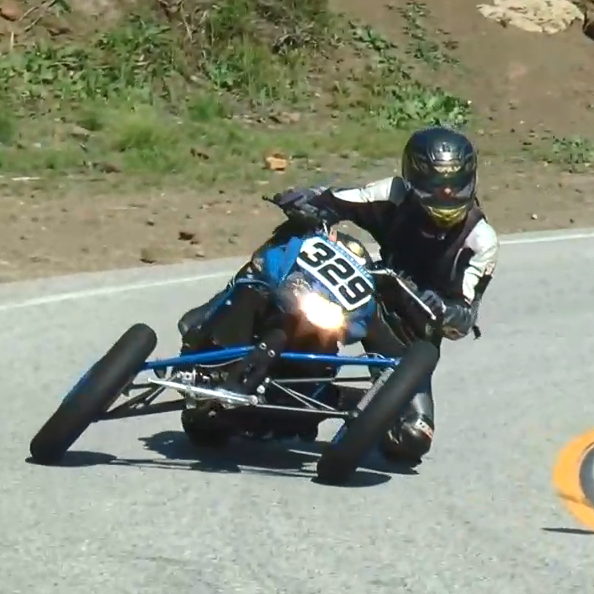
\includegraphics[width=1.0\linewidth]{figs/02/passive}
	\caption{Passive tilting system from \textit{Tilting Motor Works}}
\end{marginfigure}
\begin{marginfigure}
	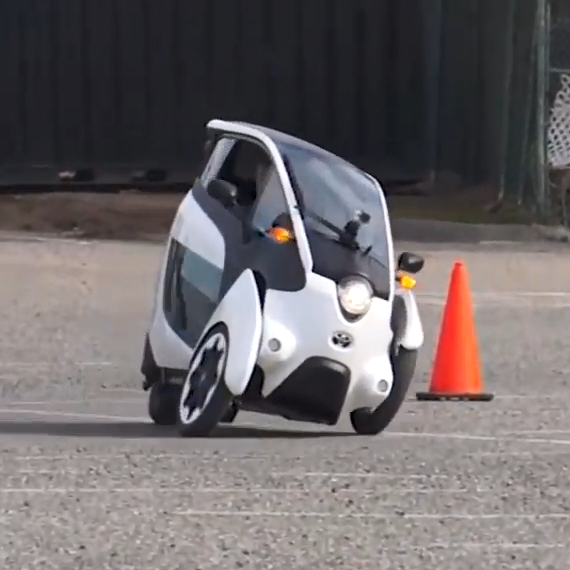
\includegraphics[width=1.0\linewidth]{figs/02/active}
	\caption{Active tilting system from the \textit{Toyota i-ROAD concept car}}
\end{marginfigure}

Thus, some of these vehicles have to tilt when turning to compensate for the effect of lateral acceleration and remain in balance. In the case of a motorcycle, it is the driver who causes the lateral movement of the motorcycle (\textbf{passive tilting}), whereas for heavy and bulky vehicles, the inclination must be automatic (\textbf{active tilting}). 

The main drawback with a passive tilting system is the necessity of a \textbf{locking mechanism to avoid the leaning} of the vehicle when standing. On the contrary, an active system does not need a locking mechanism, since is an actuated mechanism. In addition, the ability to control the leaning can facilitate users to get on the vehicle by leaning to one side and returning to the vertical position to start the ride.

Theferore, this problem of \textbf{stability in the curves} is a major technological challenge for these narrow vehicles. Some manufacturers have solved the difficulty by lowering the center of gravity of the vehicle to a minimum (see Tango\cite{tango} or Twizy\cite{twizy}), for example by placing the batteries very low if it is an electric vehicle. 

In the case of narrow active tilting vehicles, different actuating and control strategies have been studied in the industry, which are presented below (DTC, STC or SDTC).

\section{Narrow Three-Wheeled Vehicles}

In this section narrow tilting vehicles with three wheels are presented. In order to easily identify the different types, the following notation is adopted: \textbf{[ nF, tT, pP, S ]} with n the number of front wheels, t the number of tilting wheels, p the number of passengers and S the maximum speed in $Km / h$.

\begin{itemize}
	\begin{itemize}
	\item \textbf{GM Lean Machine}\cite{leanmachine} (1F, 1T, 1P, 125) was developed by Frank Winchell of General Motors in the early 1980's. The lateral stability of the vehicle had to be ensured by the driver, through a pedal that controlled the tilt. 

	\item \textbf{Mercedes Life Jet F300}\cite{f300} (2F, 3T, 2P, 210) was introduced in 1997 by Mercedes-Benz at the Frankfurt Motor Show. The tilt was automated through hydraulic actuators. 
	
	\item \textbf{CLEVER}\cite{clever} (1F, 1T, 2P, 80), was developed at the University of Bath (UK) in collaboration with BMW. The inclination of the front module of the vehicle is possible thanks to the hydraulic actuators linking the cab to the non-tilting rear part. The first prototypes were built in 2006, but the transient behavior of this vehicle did not always guarantee lateral stability.
	
	\item \textbf{Carver One}\cite{ClassAvec04} (1F, 1T, 2P, 185), a three-wheel tilting vehicle, born from a first aerodynamic concept. The Carver One is equipped with an automotive power unit and therefore with a wide non-tilting rear axle. The dynamics of the vehicle are based on the patented 'Dynamic Vehicle Control' technology, which is said to ensure vehicle stability by tilting the vehicle. 
	
	\item \textbf{Piaggio MP3 Hybrid 300IE}\cite{piaggio} (2F, 3T, 1P, 145), is a three-wheeled scooter with a parallel "hybrid" propulsion, based on a 125 cc engine and a 3.4 hp electric motor. Like a traditional scooter, this vehicle is tilted directly by the driver. 
		\end{itemize}
\end{itemize}

Paying attention to more lightweight vehicles (bike-like):
	
\begin{itemize}
	\begin{itemize}
	\item \textbf{Veleon}\cite{veleon} (2F, 3T, 1P, 25) both cargo and driver lean into the curve, helping to whoosh cars and other obstacles, including tight corners at high speed. The mode can be deactivated by pressing a button and the bicycle stays in vertical position.
	
	\item \textbf{Trego}\cite{trego} (2F, 3T, 1P, 25) is a successful fusion of a cargo bike and a folding bike, a modular separable tricycle. Combines a rear wheel to two front wheels, that are connected by an L structure, being extremely useful for transporting bulky items.
	
	\item \textbf{Kaylad-e}\cite{kaylad} (2F, 3T, 1P, 25) is a tilting trike concept with a 250-W electric motor and a lithium battery. The concept also includes a secure luggage holder or and optional heavy-duty container that can be mounted on the front of the bicycle.

	\item \textbf{Carqon}\cite{carqon} (2F, 3T, 1P, 30) has a patented carving mechanism underneath the frame and is equipped with a high torque motor for maximum torque and performance. It is similar to riding a normal bicycle where the driver uses his/her body to control the steering more than actually the turning of the handlebar.
}
	\\[5pt]
	\end{itemize}
\end{itemize}

\begin{marginfigure}
	\caption{Tilting Vehicles}
\end{marginfigure}

\begin{figure*}[h]
		\minipage{0.32\textwidth}
		  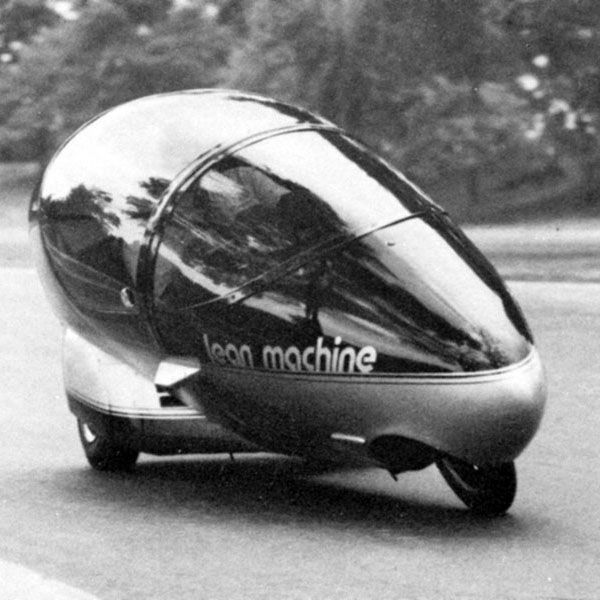
\includegraphics[width=1.0\linewidth]{figs/02/gmlean}
		  \captionof{a)}{ GM Lean Machine}
		\endminipage\hfill
		\minipage{0.32\textwidth}
		  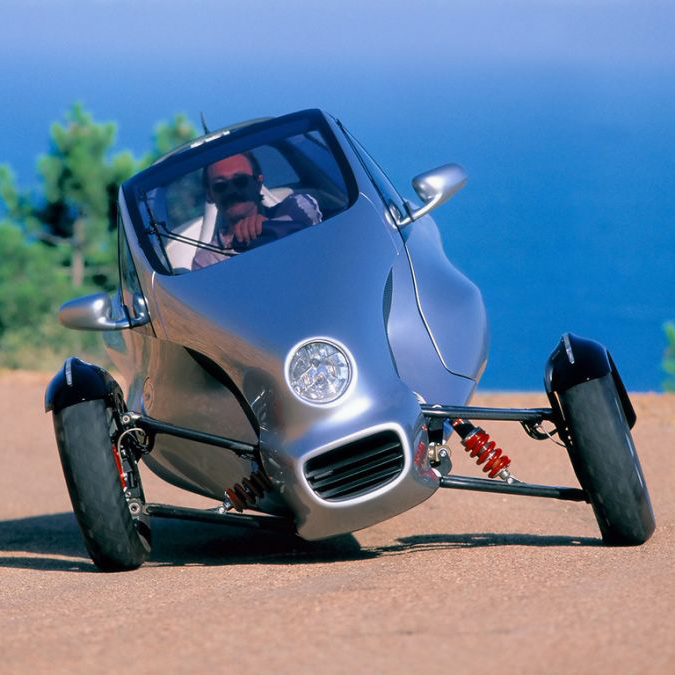
\includegraphics[width=1.0\linewidth]{figs/02/mercedes}
		  \captionof{b)}{ Mercedes Life Jet F300}
		\endminipage\hfill
		\minipage{0.32\textwidth}%
		  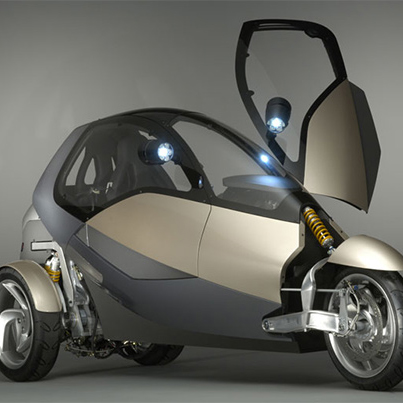
\includegraphics[width=1.0\linewidth]{figs/02/clever}
		  \captionof{c)}{ CLEVER}
		\endminipage
		\\[0pt]
\end{figure*}
		  
\begin{figure*}[h]
		\minipage{0.32\textwidth}
		  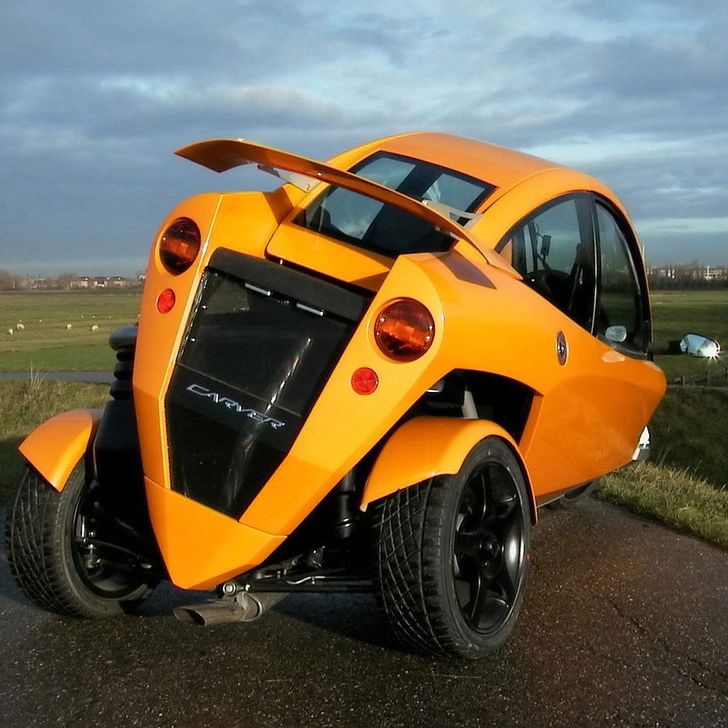
\includegraphics[width=1.0\linewidth]{figs/02/carver}
		  \captionof{d)}{ Carver One}
		\endminipage\hfill
		\minipage{0.32\textwidth}
		  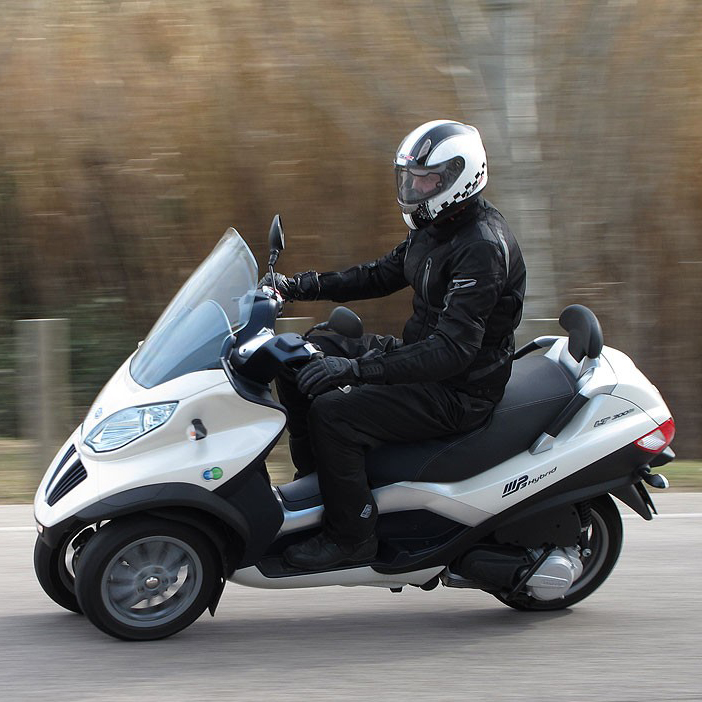
\includegraphics[width=1.0\linewidth]{figs/02/piaggio}
		  \captionof{e)}{ Piaggio MP3 Hybrid 300IE}
		\endminipage\hfill
		\minipage{0.32\textwidth}%
		  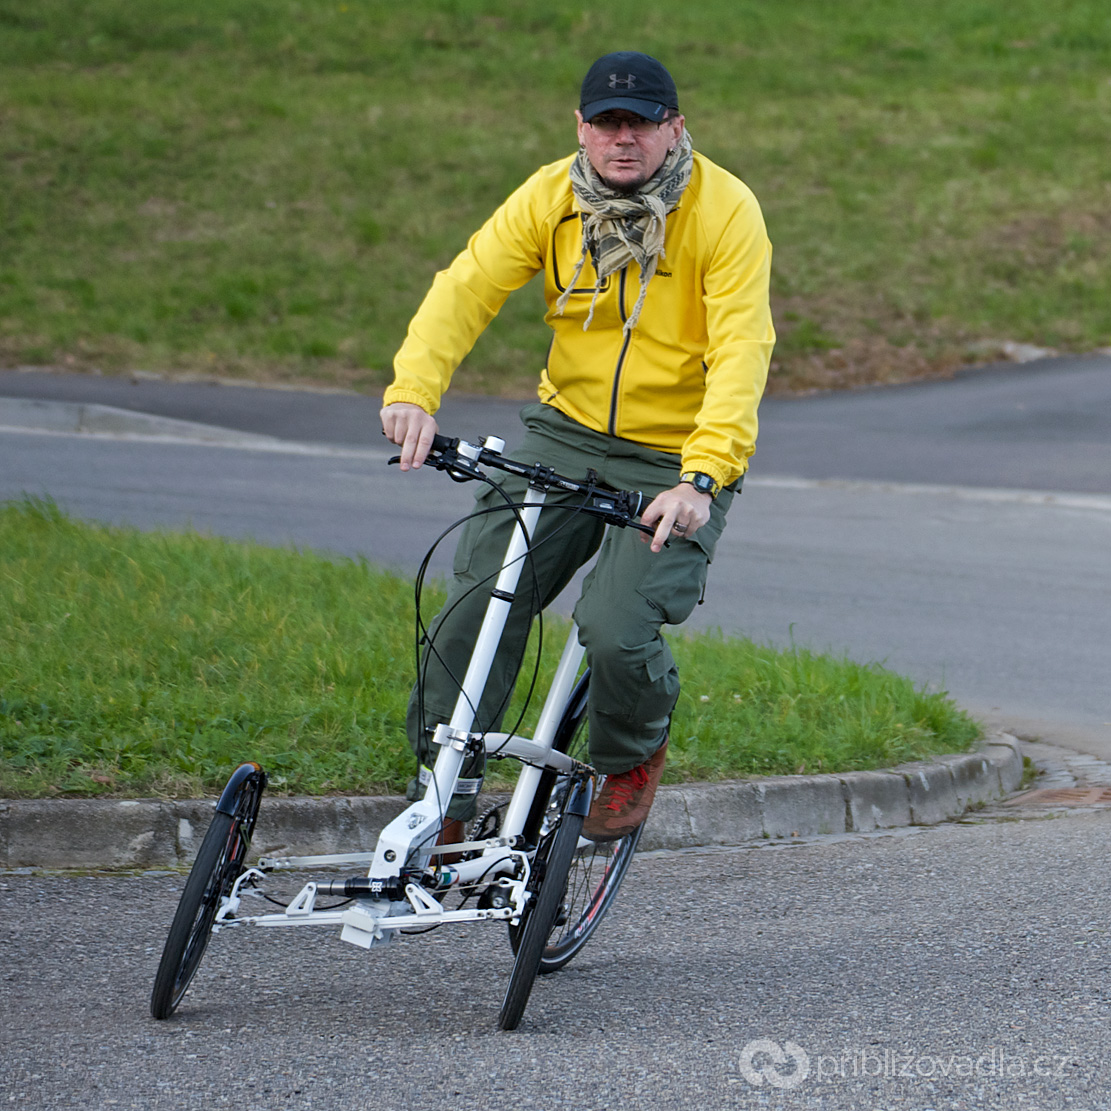
\includegraphics[width=1.0\linewidth]{figs/02/veleon}
		  \captionof{f)}{ Veleon}
		\endminipage
		\\[0pt]
\end{figure*}

\begin{figure*}[!h]
		\minipage{0.32\textwidth}
		  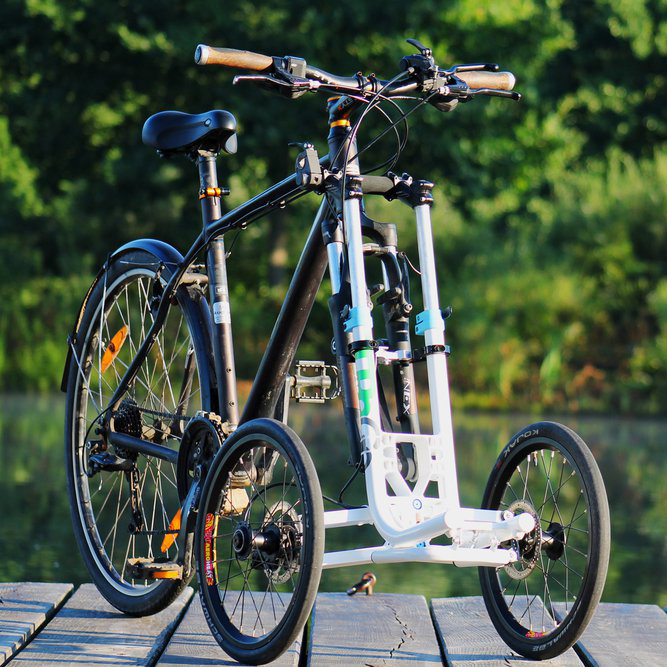
\includegraphics[width=1.0\linewidth]{figs/02/trego}
		  \captionof{g)}{ Trego}
		\endminipage\hfill
		\minipage{0.32\textwidth}
		  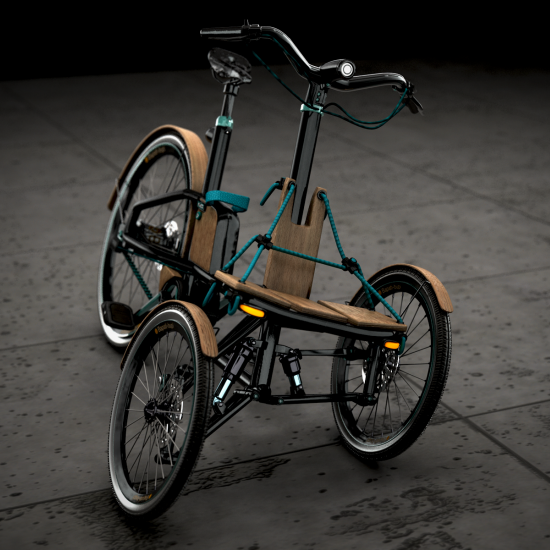
\includegraphics[width=1.0\linewidth]{figs/02/kaylad}
		  \captionof{h)}{ Kaylad-e}
		\endminipage\hfill
		\minipage{0.32\textwidth}%
		  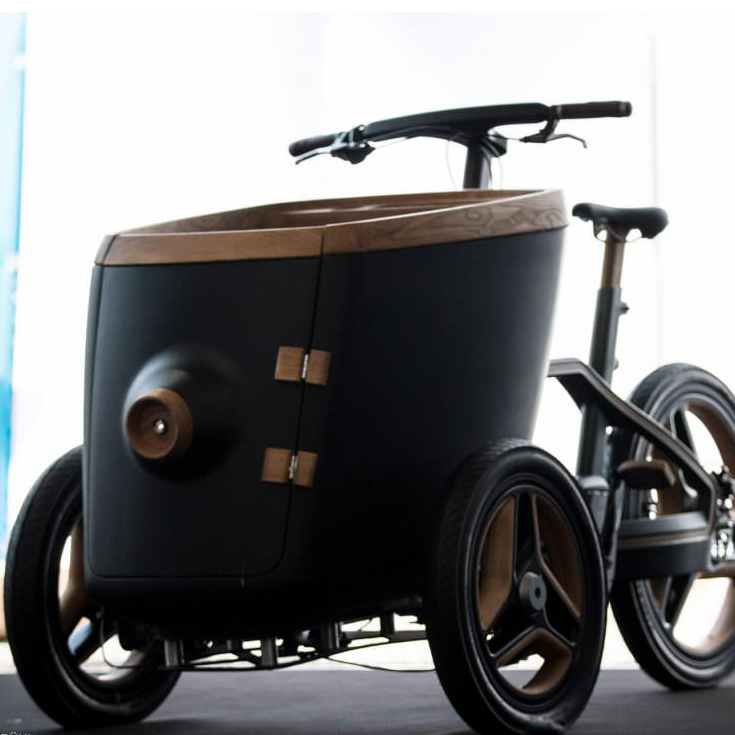
\includegraphics[width=1.0\linewidth]{figs/02/carqon}
		  \captionof{i)}{ Carqon}
		\endminipage
\end{figure*}

\newpage

\section{Tilt-Actuating Architectures}
\subsection{Direct Tilt Control (DTC)}

The inclination is achieved by means of actuators mounted directly on the longitudinal axis of the vehicle, \textbf{providing a torque} ($M_t$) to tilt the whole vehicle or some parts of it. It is the most used system on narrow tilting vehicles and the simplest active system to implement.

\begin{marginfigure}
	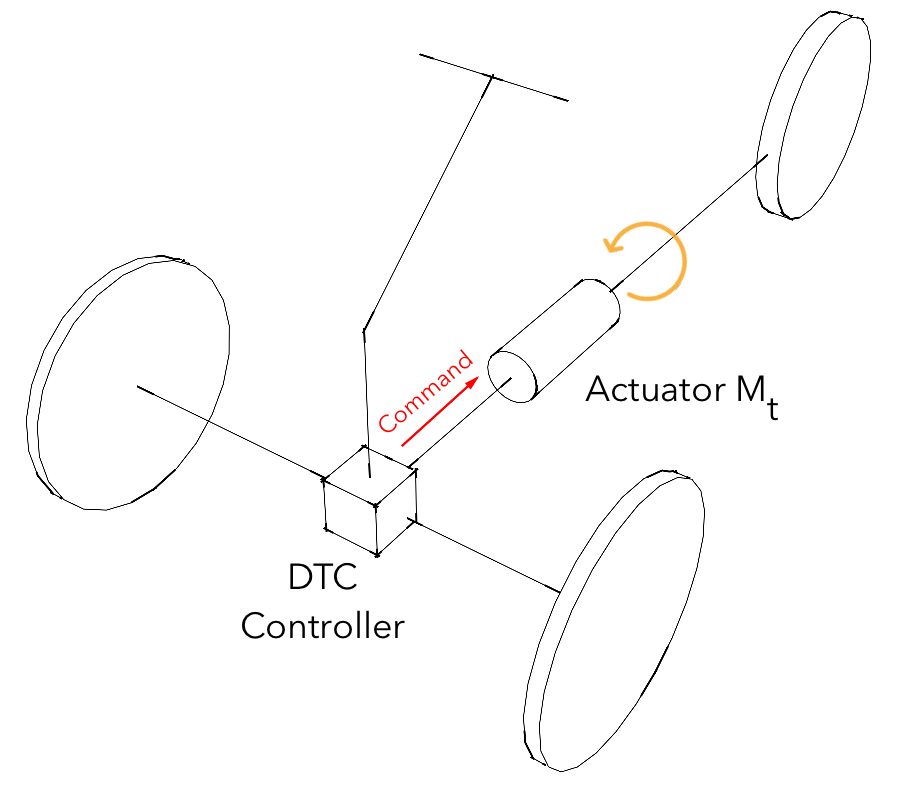
\includegraphics[width=1.0\linewidth]{figs/02/dtc_diagram}
	\caption{DTC system schematic}
\end{marginfigure}

In a turn, the lateral acceleration is proportional to the longitudinal velocity, as is demonstrated in the next chapter. Therefore, for the same steering angle, the lateral acceleration is higher at high speed. As a result, the \textbf{torque $M_t$ required is greater at high speed} since it must ensure the desired inclination in the opposite direction to that of the lateral acceleration. 

It is at high speed that there is a greater risk of \textbf{saturation of the actuator}. It should be noted that if the DTC system only acts from the measurement of the measured acceleration, this may cause an unpleasant feeling in the passengers. When driving a motorcycle, the rider tilts the vehicle simultaneously with the taking of the turn, so that the perceived acceleration remains virtually zero, even in transient situations.

\subsection{Steering Tilt Control (STC)}

These systems control the steering angle of the wheels. The steering angle ($\delta_{driv}$) applied by the driver is modulated by the STC system ($\delta_c$) to control the tilt angle using countersteering. This strategy is inspired by the action of a bicycle or motorcycle rider, but is seldom used by manufacturers, since it is based on a \textbf{steer-by-wire} system, which is still prohibited to commercialize for safety standards reasons.

\begin{marginfigure}
	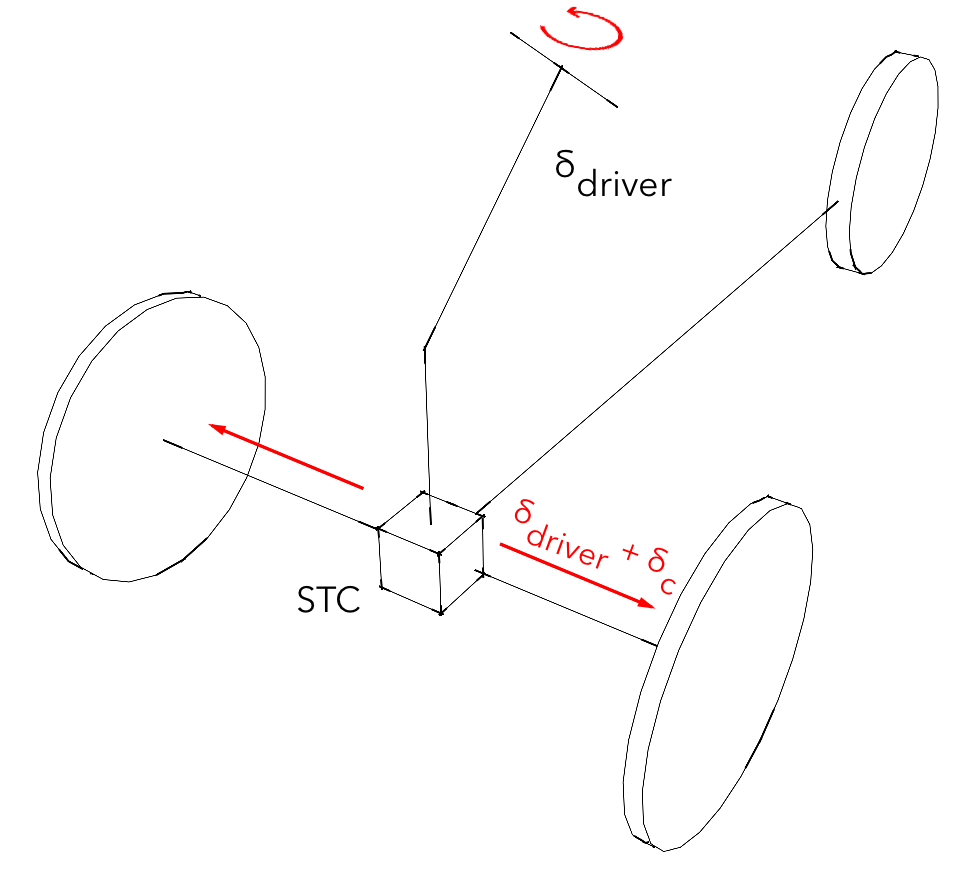
\includegraphics[width=1.0\linewidth]{figs/02/stc_diagram}
	\caption{STC system schematic}
\end{marginfigure}

STC systems are not well suited for \textbf{low longitudinal speeds}, demanding a large counter-steering to tilt the vehicle, which deviates it significantly from its trajectory. In contrast, the STC system is more efficient than the DTC at high speed, as a large torque is required by the DTC (due to the delay in the DTC tilting torque).
\newpage

\subsection{Comparison between DTC and STC}

Let us compare both tilting systems by looking to the forces actuating in each case. The vehicle is traveling in an straight line at a constant velocity $V$, when a right turn comes.


	
\begin{itemize}
	\begin{itemize}
	\item DTC: the driver will turn the steering wheel to the right (Figure \ref{dtc}), producing a lateral acceleration in the inner direction of the curve( do not confuse it with the inertial force which pushes the vehicle outwards the curve). Due to the possibility of tilting, the vehicle will tend to lean to the left, but in this moment the DTC torque $M_t$ will correctly lean it to the right. In this simple case it is clear the delay between the lateral acceleration and the torque $M_t$.
	\begin{figure}[h]
		\minipage{0.32\textwidth}
		  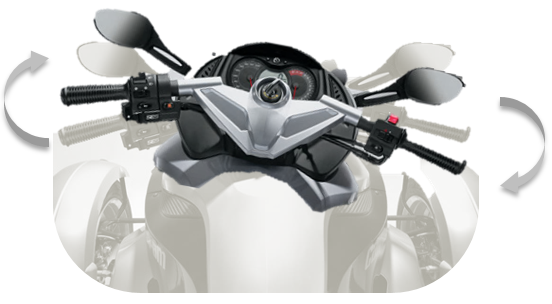
\includegraphics[width=1.0\linewidth]{figs/02/dtc_1}
		\endminipage\hfill
		\minipage{0.32\textwidth}
		  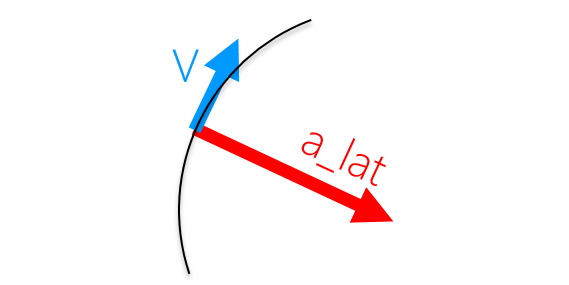
\includegraphics[width=1.2\linewidth]{figs/02/dtc_2}
		\endminipage\hfill
		\minipage{0.32\textwidth}%
		  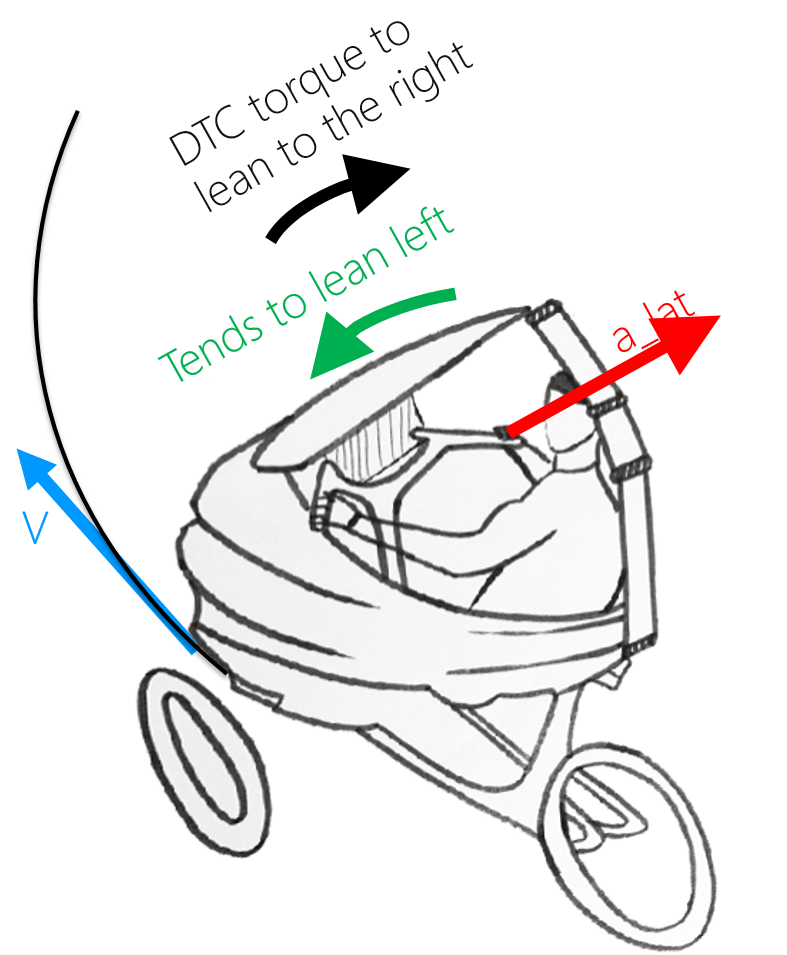
\includegraphics[width=1.0\linewidth]{figs/02/dtc_3}
		\endminipage
		\label{dtc}
		\caption{Direct Tilt Control \protect\\ a) Steering input from the driver \protect\\ b) DTC force diagram in a right turn \protect\\ c) DTC tilting torque input}
		\\[1pt]
	\end{figure}
	\item STC: the STC steer-by-wire system will slightly turn the steering wheel to the left (Figure \ref{stc}), producing a lateral acceleration in the outer direction of the curve. Due to the possibility of tilting, the vehicle will correctly lean to the right. By using the countersteering, the vehicle easyly leans to the appropiate side, but the desired path of the user is not perfectly followed.
	\begin{figure}[h]
		\minipage{0.32\textwidth}
		  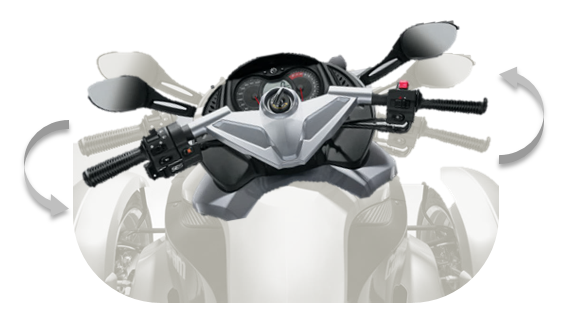
\includegraphics[width=1.0\linewidth]{figs/02/stc_1}
		\endminipage\hfill
		\minipage{0.32\textwidth}
		  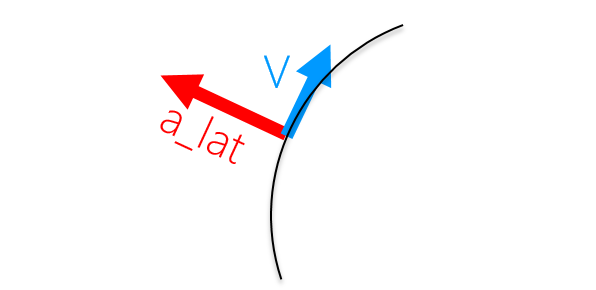
\includegraphics[width=1.2\linewidth]{figs/02/stc_2}
		\endminipage\hfill
		\minipage{0.32\textwidth}%
		  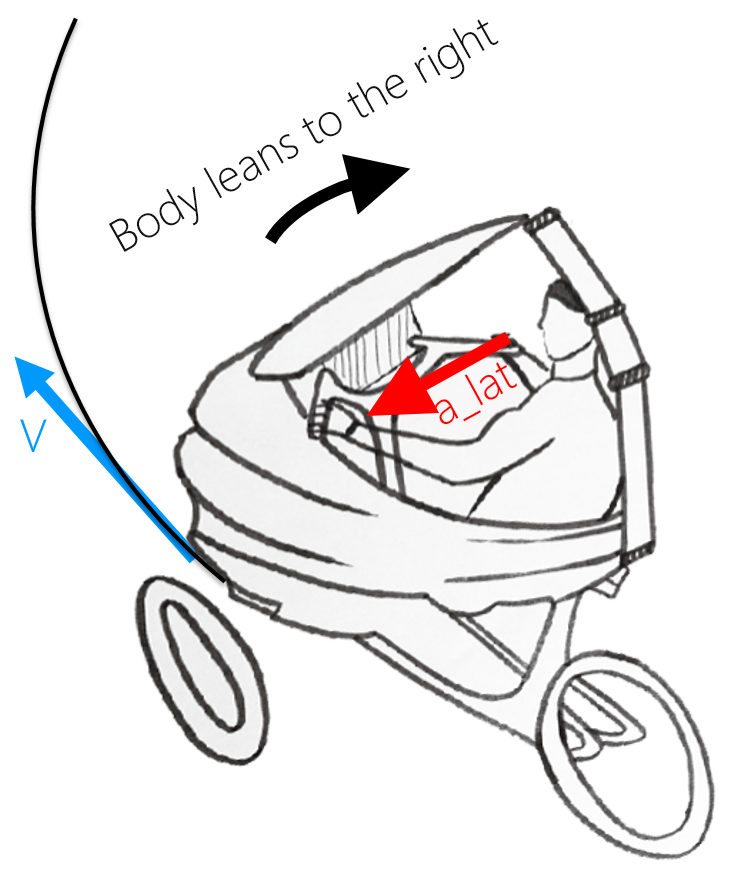
\includegraphics[width=1.0\linewidth]{figs/02/stc_3}
		\endminipage
		\caption{Steering Tilt Control: \protect\\a) Steering input from the actuator \protect\\b) STC force diagram in a right turn \protect\\c) STC tilts automatically in a right turn}
		\label{stc}
	\end{figure}
	\end{itemize}
\end{itemize}
\newpage
In order to give an overall view, the table \ref{dtc_vs_stc} summarizes the characteristics of the two systems DTC and STC.
\begin{table*}[h]
\centering
\caption{DTC vs STC comparison table}
\label{dtc_vs_stc}
	\begin{tabular}{l|c|c|}
	           & \textbf{DTC}                                   & \textbf{STC}                  \\
	\hline        
	\textbf{Lean by}    & Roll actuator                         & Countersteering                 \\
	\textbf{Stability}  & Always stable                         & Unstable at low speeds          \\
	\textbf{High Speed} & Deal with high lateral acceleration   & Small adjustments               \\
	\textbf{Low Speed}  & Good behaviour at low speeds: $M_t$ \Uparrow & Large and frecuent steer inputs $\delta_c$ \Uparrow
	\end{tabular}
	\\[20pt]
\end{table*}

\subsection{SDTC hybrid solution}
To take advantage of both strategies and their complementary efficiencies according to speed, recent work has focused on the so-called SDTC hybrid solution for vehicles with both a tilt actuator and a steer-by-wire system. The first solutions are monovariable, meaning that a single control input is active at a time, with switching from one system to the other as a function of the speed. 

The STC systems are generally implemented from a threshold speed of approximately $V=40 Km/h$ while the DTC systems are active below that speed. Switching from one system to another by switching is complicated due to the fact that the control signals act as antagonist in transient phases\cite{doi:10.1080/00423119708969321},\cite{hibbard1996twenty}.
\begin{itemize}
	\begin{itemize}
	\item In transient, the STC system causes a counter-steering, and the created lateral acceleration created serves for the inclination of the vehicle. Switching from STC to DTC, the DTC command will seek to tilt the vehicle in the opposite direction to the perceived lateral acceleration, hence in the wrong direction. The two control signals are conflicting or antagonistic in this case.

	\item Switching from DTC to STC, the control signals are not conflicting, but the tilt torque DTC $M_t$ abruptly cancels out as the vehicle starts to tilt. This interruption creates a discontinuity and peaks in the signals.
	\end{itemize}
\end{itemize}

\newpage

\section{Vehicle Model}
Modeling is a key step in the study and control of systems. Depending on the use to be made (embedded model, design model, simulation model...), different levels of complexity can be envisaged.

\subsection{Models Used in the Literature}
The study and development of narrow vehicles only began recently, due to the congestion problems of road traffic and the increase in pollution. The problem of narrow and tilting vehicles is therefore recent, and few research teams have worked on this subject. The \textbf{narrow tilting vehicle models} will be reviewed in this section, explaining their advantages and limitations. 

Researchers at \textbf{California University} were among the first to take an interest in this matter. In Hibbard R. \textit{et al.}, (1996)\cite[-4.5cm]{hibbard1996twenty} and So S. \textit{et al.}, (1997a)\cite[-1.7cm]{doi:10.1080/00423119708969321}, the authors consider only the dynamics of the angle of inclination $\theta$, and the model used for the simulation was reduced to the transfer function between the input $M_t$ and $\theta$. 

A more detailed linearized simulation model at small angles, with longitudinal dynamics, was used in later work (So S. \textit{et al.}, 1997b)\cite[-1.7cm]{doi:10.1504/IJVD.1997.062071}.

In the UK, at the \textbf{University of Bath}, the researchers worked on the CLEVER project. In his thesis\cite[-0.3cm]{bath24682}, J. Berote focused on the vehicle modeling, developing a 5 degree of freedom (dof) multi-body model, that included dynamics of hydraulic actuators, which was then incorporated into the SimMechanics software to obtain a validation model. 

Previously, they used a PID controller (J. Berote \textit{et al.}, 2008)\cite[-1cm]{bath15090}, that did not require any model. For such a purpose, the authors considered approximate relations between the steering angle and the lateral acceleration, and between the steering angle and the angle of inclination. 
\\
\begin{figure}[h!]
	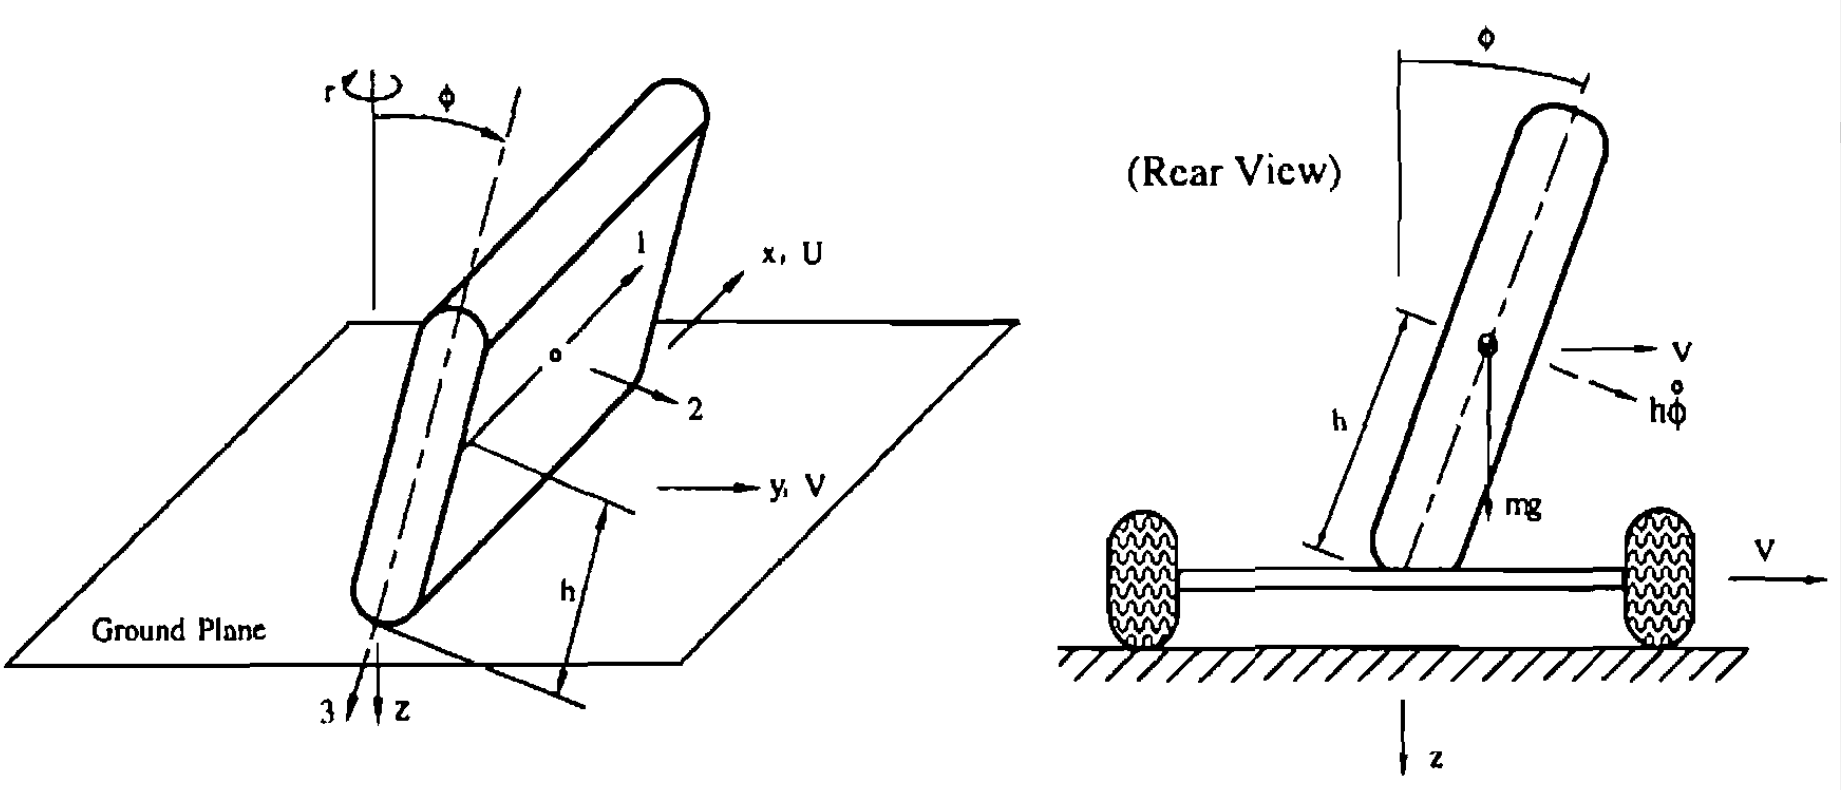
\includegraphics[width=1.0\linewidth]{figs/02/literature_model}
	\caption{Literature model: Inverted pendulum simple model for tilting vehicles }
	\label{literature}
	\\[-3cm]
\end{figure}

\newpage

At the \textbf{University of Minneapolis} in Minnesota, a prototype recliner was built, and several advances were made. In the article R. Rajamani \textit{et al.}, (2003)\cite[0cm]{doi:10.1076/mcmd.9.2.209.16521} the authors focus on modeling the vehicle. They neglect the longitudinal dynamics, but take into account the gyroscopic moments of the wheels and the tilting moment. 

Their synthesis model for the design of the control law, also used for simulation, was later simplified and a linearized model of equation (Piyabongkran D. \textit{et al.} 2004\cite{piyabongkarn2004active}, Kidane S. \textit{et al.}, 2010\cite{5356230}, Kidane S. \textit{et al.}, 2008\cite{doi:10.1080/00423110701352987}}).



%In France, at the \textbf{Ecole des Mines de Nantes}, L. Mourad et al.
%\newpage
\subsection{Bicycle Model}

The lateral control of the tilting vehicles is the object of this study. The so-called \textbf{bicycle model} has been chosen to be considered as a conceptual model which aggregates the 2 front wheels in one wheel, and only one rear wheel. Wheel torques are also simplified. They are implicitly replaced by the steering angle. 

This model has been built from the 4 dof model presented in the article of R. Rajamani \textit{et al.}, (2003)$^{19}$, which considers the longitudinal speed as a parameter of the model and not as a state variable.

The model obtained takes into account the longitudinal dynamics relating to the speed, as well as the lateral dynamics including the inclination. Figures \ref{xy} and \ref{yz} respectively show the views in the horizontal ($XY$) and vertical ($YZ$) planes of the vehicle. 

The quantities and notations used below are defined in the 'Notations' section at the beginning of the thesis. Let us define the following coordinate systems: 
\begin{enumerate}
\item The absolute coordinate system $R$=($X$, $Y$, $Z$) fixed to the ground, the axes $X$ and $Y$ are on the ground while the $Z$ is the vertical axis. 

\item The vehicle coordinate system $r$=($x$, $y$, $z$) is linked to the vehicle. Its origin is the point G (center of gravity), the axis $x$ is parallel to the longitudinal axis of the vehicle, the axis $z$ is parallel to the axis $Z$ and the axis $y$ is such that the planes $xy$ and $XY$ are parallel.

\item The coordinate system  $r'$=($x'$, $y'$, $z'$) is linked to the frame and tilts with it. It coincides with the reference mark ($x$, $y$, $z$) when the vehicle is in vertical position. Its axes $y'$ and $z'$ are inclined by an angle $\theta$ equal to the angle of inclination of the vehicle. 

%\item The coordinate system $r_v$=($x_v$, $y_v$, $z_v$) is at the center of gravity G of the vehicle, with the axis $x_v$ collinear and in the same direction as the speed of the vehicle; The vertical axis $z_v$ is parallel to the axis $Z$, and the axis $y_v$ forms a direct trihedron with $x_v$ and $z_v$.
\end{enumerate}

\newpage
\begin{figure*}[h!]
	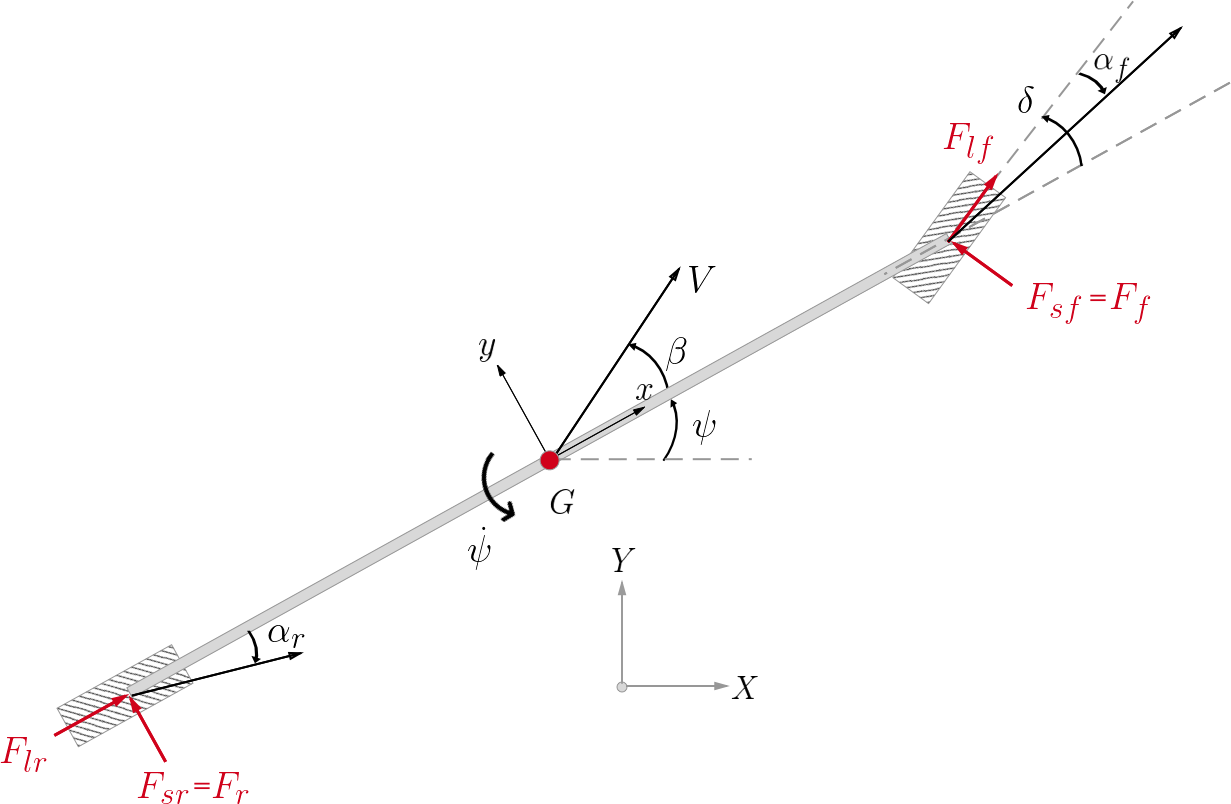
\includegraphics[width=1.0\linewidth]{figs/02/xy1}
	\caption{Bicycle model: View of the plane $XY$}
	\label{xy}
\end{figure*}

The vehicle has 3 degrees of freedom (listed below) and takes into account the effects of trail, slip angles and gyroscopic effects.

$y$ \quad Lateral position with respect to road reference \\
$\psi$ \quad Yaw angle \\ 
$\theta$ \quad Tilt angle \\
%$\delta$ \quad Front wheel steering angle 
\subsection{Model Equations}
The equations of the model implemented in this thesis have been derived using one principle:

\begin{itemize}
	\begin{itemize}
	\item The \textbf{fundamental principle of dynamics in translation and rotation}, also called Newton's laws, which require knowledge of the mechanical connections of all internal and external forces acting on the vehicle, and their points of application:
	\[\sum_{i} F=ma,\quad \sum_{j} M=I\ddot{\theta}\]
	Where $F$ represents the external forces applied to the body, $i$ the number of these forces, $m$ its mass and $a$ its acceleration. $M$ the external moments applied to the body, $j$ the number of these moments, $I$ its inertia, and $\ddot{\theta}$ its angular acceleration.
%\item The \textbf{principle of the least action and the Lagrange formalism} based on the calculation of the kinetic energy $T$ and potential $V$:
%	\[L=T-V,\quad \frac{d}{dt}\frac{\partial L}{\partial \dot{q_{i}}}-\frac{\partial L}{\partial q_{i}}=F_{q_{i}}\]
%	Where $q_{i}$ are the generalized coordinates.
	\end{itemize}
\end{itemize}
\begin{figure}
	\centering
	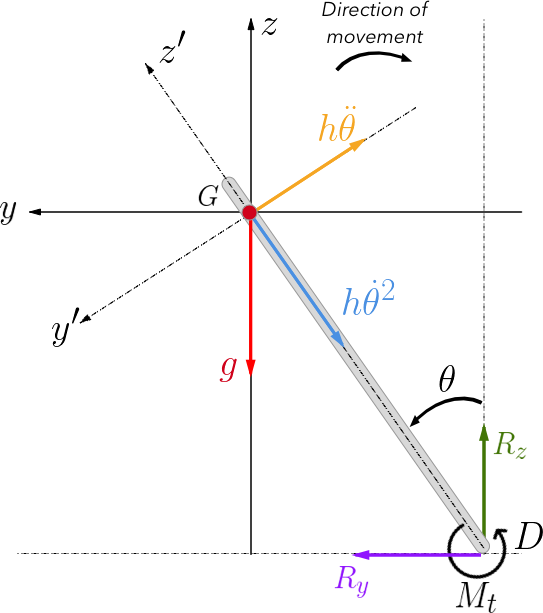
\includegraphics[width=0.85\linewidth]{figs/02/yz2}
	\caption{Bicycle model: View of the plane $YZ$}
	\label{yz}
\end{figure}
Applying Newton's principle to the presented bicycle model:\\
\minipage{0.5\textwidth}
	\[\sum_{i} \vec{F}=m\vec{a}\]
\endminipage\hfill
\minipage{0.5\textwidth}
	\begin{eqnarray}
	y) \quad R_{y}=m\,a_{y} \\
	z) \quad R_{z}-mg=m\,a_{z}
	\end{eqnarray}
\endminipage\hfill
\minipage{0.5\textwidth}
	\[\sum_{j} \vec{M}=I\vec{\ddot{\theta}}\]
\endminipage\hfill
\minipage{0.5\textwidth}
	\begin{eqnarray}
	x) \quad I_{x} \ddot{\theta}=R_{z}\,h\,\sin {\theta}\,-\,R_{y}\,h\,\cos {\theta} \\
	z) \quad I_{z} \ddot{\psi}=F_{f}\,L_{f}-F_{r}\,L_{r}
	\end{eqnarray}
\endminipage\hfill

The absolute acceleration (in the inertial reference frame $R$) of a moving body can be decoupled in two terms if a non-inertial frame of reference $r$ is attached to the body. 

Hence, the accelerations $a_{y}$ and $a_{z}$ can be obtained from the acceleration of the point $D$ (in contact with the ground), plus the relative accelerations of the center of gravity $G$ with respect to the point $D$:
\begin{eqnarray}
a_{y}=a_{D,y}+a_{G/D,y}\\
a_{z}=a_{D,z}+a_{G/D,z}
\end{eqnarray}
The center of gravity $G$ describes a circular arc of center $D$ at speed $v_{G}=h\dot{\theta}$ with $\bar{DG}=h$. The accelerations experienced at G are the tangential acceleration $\frac{dv_{G}}{dt}=h\ddot{\theta}$ along the axis $y'$, and the normal acceleration $-h\dot{\theta}^2$ along the axis $z'$.
By projecting these equations on the axes of the reference $r$=($x$, $y$, $z$):
\[a_{D,y}=\ddot{y}+V \dot{\psi}\]
\[a_{D,z}=0\]
\begin{marginfigure}[-3cm]
	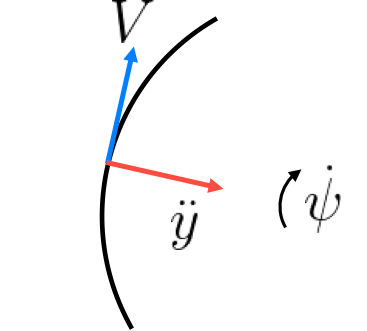
\includegraphics[width=0.8\linewidth]{figs/02/circular}
	\caption{Circular path velocity and lateral acceleration}
\end{marginfigure}

\newpage
If $D$ is taken into account as a fixed point, the relative motion can be considered:
\[v_{G}=v_{D}+\vec{w} \wedge \vec{DG}=0 + \dot{\theta}\,h(\cos {\theta}\,\vec{j}-\sin {\theta}\,\vec{k})\]
\[a_{G}=a_{D}+\vec{\alpha}\wedge\vec{DG}-w^2\,\vec{DG}=0 + \ddot{\theta}h(\cos {\theta}\,\vec{j}-\sin {\theta}\,\vec{k})-\theta^2 h (\sin {\theta}\,\vec{j}-\cos {\theta}\,\vec{k})\]
\[a_{G/D,y}=\ddot{\theta}h \cos {\theta} - \theta^2 h \sin \theta\]
\[a_{G/D,z}=-\ddot{\theta}h \sin {\theta} - \theta^2 h \cos \theta\]
Having studied the relative motion, the absolute accelerations are expressed as:
\begin{eqnarray}
a_{y}=a_{D,y}+a_{G/D,y}=\ddot{y}+V \dot{\psi}+\ddot{\theta}h \cos {\theta} - \theta^2 h \sin \theta \\
a_{z}=a_{D,z}+a_{G/D,z}=-\ddot{\theta}h \sin {\theta} - \theta^2 h \cos \theta
\end{eqnarray}
Therefore, replacing these expressions into equations (1), (2) and (3):
\[R_{y}=m\,a_{y}=m(\ddot{y}+V \dot{\psi}+\ddot{\theta}h \cos {\theta} - \theta^2 h \sin \theta)\]
\[R_{z}=m\,(a_{z}+g)=m(-\ddot{\theta}h \sin {\theta} - \theta^2 h \cos \theta + g)\]
\[I_{x} \ddot{\theta}=mh(-\ddot{\theta}h \sin^2 {\theta} - \theta^2 h \sin \theta \cos \theta + g \sin \theta -\ddot{y}\cos \theta-V \dot{\psi}\cos \theta-\ddot{\theta}h \cos^2 {\theta} + \theta^2 h \sin \theta \cos \theta)\]

The last equation represents the roll motion, and since it is going to be actuated by the motor, the tilting torque $\textcolor{blue}{M_{t}}$ has been included.
\[I_{x} \ddot{\theta}=mh(-\ddot{\theta}h + g \sin \theta -\ddot{y}\cos \theta-V \dot{\psi}\cos \theta) \textcolor{blue}{+M_{t}}\]
To get equation (4), the moment equilibrium is calculated in the c.g. Figure \ref{yaw} illustrates the vehicle from the top view, with the lateral tire forces $F_{f}$ and $F_{r}$.
\begin{equation}
I_{z} \ddot{\psi}=F_{f}\,L_{f} - F_{r}\,L_{r}
\end{equation}
\begin{marginfigure}[-5cm]
	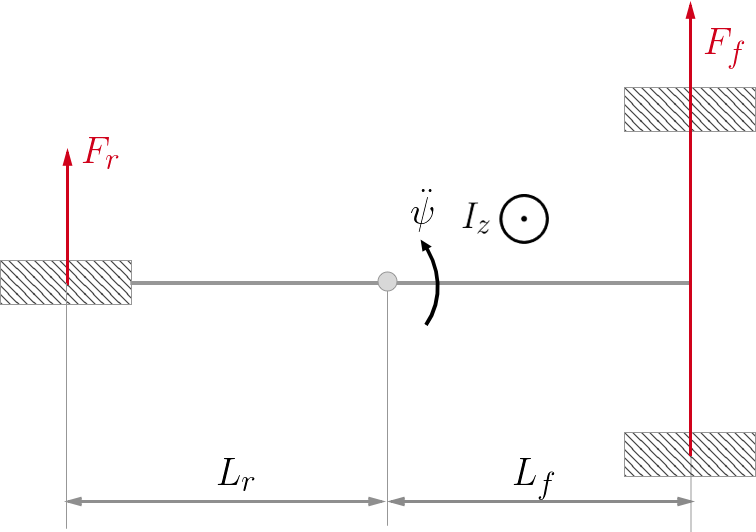
\includegraphics[width=1.2\linewidth]{figs/02/top}
	\caption{Lateral tire forces and yaw dynamics}
	\label{yaw}
\end{marginfigure}
The lateral force exerted on a wheel is expressed as $F=C\alpha + \lambda\theta$, where $C$ is the coefficient of stiffness and $\lambda\theta$ is due to the camber. Using the equality $\alpha=\delta-\tan^{-1}\Big(V_{y}/V_{x}\Big)$, at the level of the front wheels, the lateral tire forces are defined as follow for small slip angles:
\begin{eqnarray}
F_{f}=2 C_{f}\Big(\delta - \frac{\dot{y}+L_{f} \dot{\psi}}{V} \Big) + 2 \lambda_{f} \theta \\
F_{r}=C_{r}\Big(- \frac{\dot{y}-L_{r} \dot{\psi}}{V} \Big) +\lambda_{r} \theta
\end{eqnarray}
where $C_{f}$ and $C_{r}$ are the cornering stiffness of the front and rear tires, and $\lambda_{f}$ and $\lambda_{r}$ the camber stiffness of each wheel. 

\newpage
\subsubsection{\textbf{Front Wheel Dynamics due to Trail}}

The axis of the wheel has so far been considered perpendicular to the plane of the ground. This is not really the case in practice, since the axis is generally slightly inclined as shown in Figure \ref{wheels}. 
\begin{marginfigure}
	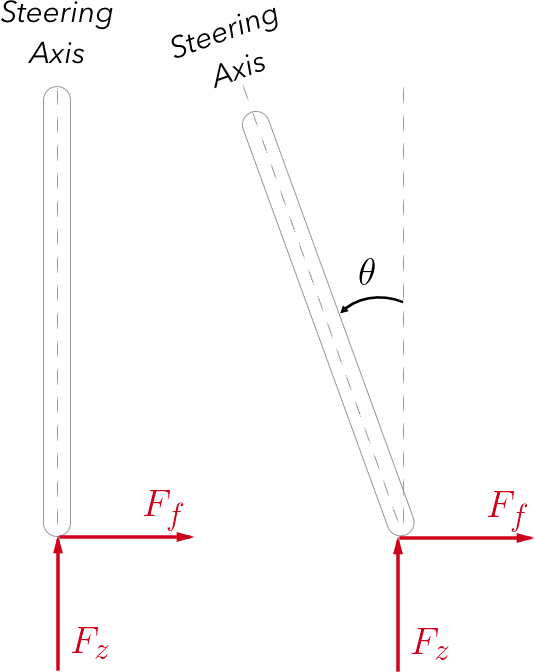
\includegraphics[width=1.0\linewidth]{figs/02/wheels}
	\caption{Inclined steering axis due to the tilting}
	\label{wheels}
\end{marginfigure}
\begin{marginfigure}
	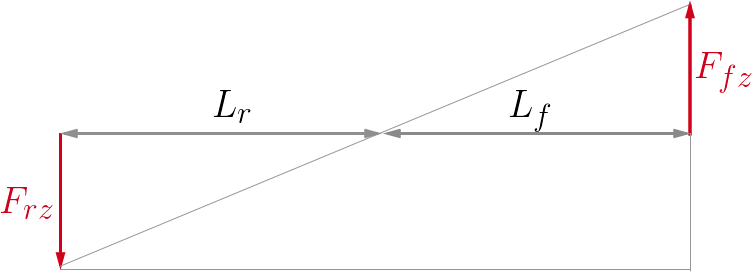
\includegraphics[width=1.2\linewidth]{figs/02/forces}
	\caption{Vertical forces diagram}
	\label{forces}
\end{marginfigure}
In absence of suspension dynamics, tilt dynamics and longitudinal acceleration, the sum of the normal forces will equal the weight of the vehicle. In addition, considering the similarity relation from Figure \ref{forces}, the normal force acting on the front wheels $F_{z}$ can be obtained:
\[\frac{F_{rz}+F_{fz}}{L_{r}+L_{f}}=\frac{F_{rz}}{L_{r}}=\frac{F_{fz}}{L_{f}}\]
\begin{equation}
F_{fz}+F_{rz}=mg \quad \Rightarrow \quad F_{fz}= F_{z}=mg \frac{L_{r}}{L_{r}+L_{f}}
\end{equation}
Thus, the reaction of the ground $F_{z}$, perpendicular to the plane of the ground, will contribute with a moment equal to $F_{z}\sin\theta$ to the steering axis. Similarly, the lateral force also contributes a restoring steering torque on the wheel (Figure \ref{trail_2}):
\begin{equation}
M_{trail}=F_{z}\gamma\cos\beta\sin\theta-F_{f}\cos\theta(\gamma+\gamma_{pneumatic})\cos\beta
\end{equation}
%\begin{marginfigure}
%	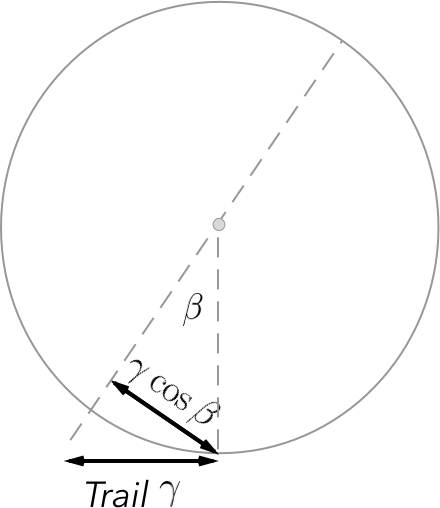
\includegraphics[width=1.1\linewidth]{figs/02/trail_1}
%	\caption{Front wheel trail}
%	\label{trail_1}
%\end{marginfigure}

\begin{figure}
	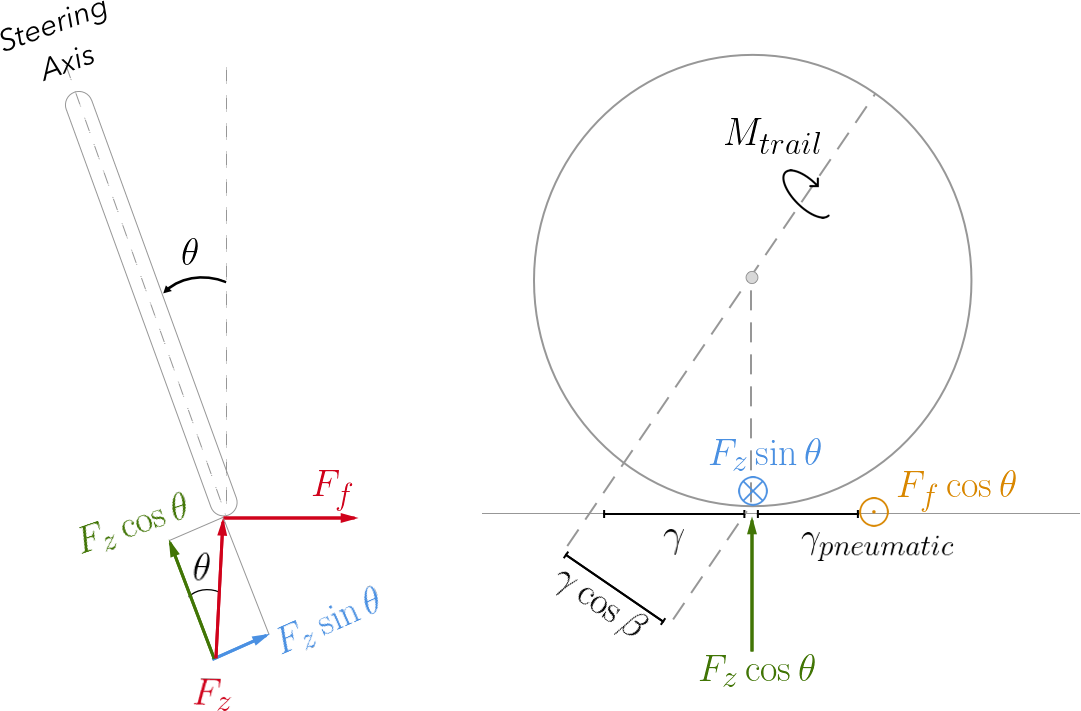
\includegraphics[width=1.1\linewidth]{figs/02/trail_2}
	\caption{Forces on front wheels when the vehicle is tilted to the left}
	\label{trail_2}
\end{figure}


\marginnote[-2.5cm]{Please notice, that the lateral force $F_f$ is not located exactly in the contact point with the ground, there exists a distance $\gamma_{pneumatic}$.}

\subsubsection{\textbf{Gyroscopic Moments}}

The dynamic equations of a rigid body with 3 rotational degrees of freedom are derived from the Euler equations:
\marginnote{Inertial reference frame:
\[\sum \vec{M}=\frac{d\vec{H}}{dt}=\frac{d(I\vec{w})}{dt} \]}
\marginnote{Non-inertial reference frame:
\[\sum \vec{M}=\Big(\frac{d(I\vec{w})}{dt}\Big)_{fixed} + \vec{w}\wedge(I\vec{w})\]}
\begin{eqnarray}
x) \quad \sum \vec{M_{x}}=I_{xx}\,\dot{\vec{w_{x}}} - (I_{yy}-I_{zz})\vec{w_{y}}\vec{w_{z}}\\
y) \quad \sum \vec{M_{y}}=I_{yy}\,\dot{\vec{w_{y}}} - (I_{zz}-I_{xx})\vec{w_{x}}\vec{w_{z}}\\
z) \quad \sum \vec{M_{z}}=I_{zz}\,\dot{\vec{w_{z}}} - (I_{xx}-I_{yy})\vec{w_{x}}\vec{w_{y}}
\end{eqnarray}

\newpage
The vehicle has two rotational degrees of freedom: yaw and roll (pitch is neglected). In addition, each rotating wheel has three rotational degrees of freedom, and Euler's equations should be applied to the rotating wheels.

Free body diagrams of the front wheels, rear wheel and vehicle body are shown in Figure \ref{body_1}. 

\begin{marginfigure}[-0.5pt]
	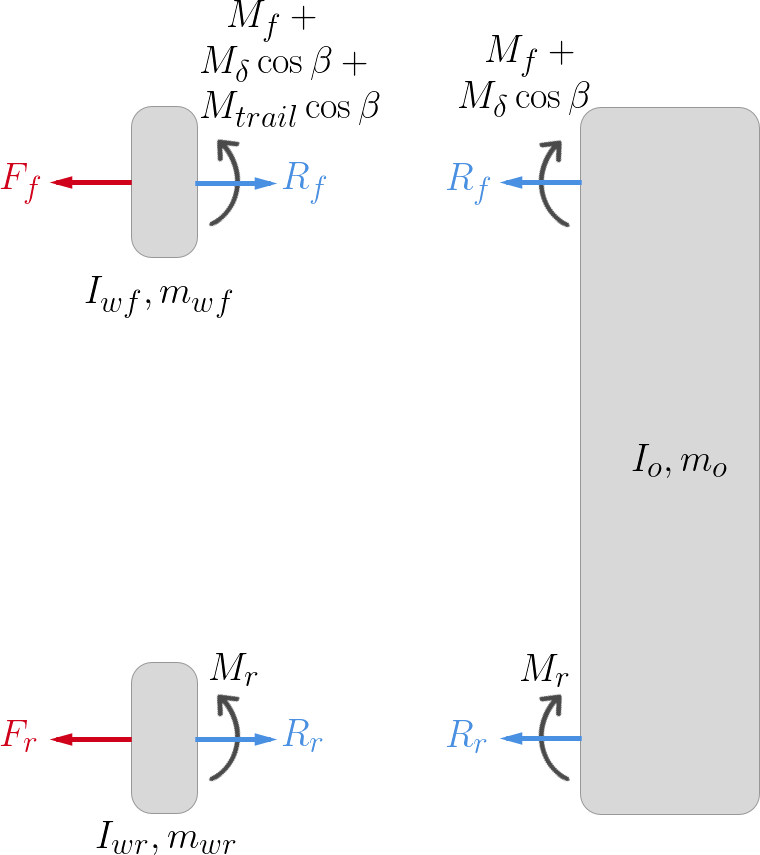
\includegraphics[width=1.3\linewidth]{figs/02/body_1}
	\caption{Free body diagram of front wheels, rear wheels and body}
	\label{body_1}
\end{marginfigure}
- \underline{Front Wheels}
\begin{eqnarray}
F_{y}) \quad 2\,m_{wf}\big(\ddot{y}+V\dot{\psi}+h_{f}\n\ddot{\theta}\cos\theta-h_{f}\dot{\theta}^2\sin\theta+L_{f}\ddot{\psi}\big)=F_{f}-R_{f} \\
M_{z}) \quad 2\,I_{wf,\psi}(\ddot{\psi}+\ddot{\delta}\cos\beta)+2(I_{wf,\theta}-I_{wf,rot})w_{rot}(\dot{\theta}-\dot{\delta}\sin\beta)=\notag\\
\quad\quad M_{f}+M_{\delta}\cos\beta+M_{trail}\cos\beta
\end{eqnarray}

- \underline{Rear Wheels}
\begin{eqnarray}
F_{y}) \quad m_{wr}\big(\ddot{y}+V\dot{\psi}+h_{r}\n\ddot{\theta}\cos\theta-h_{r}\dot{\theta}^2\sin\theta-L_{r}\ddot{\psi}\big)=F_{r}-R_{r} \\
M_{z}) \quad I_{wr,\psi}\ddot{\psi}+(I_{wr,\theta}-I_{wr,rot})w_{rot}\dot{\theta}=M_{r}
\end{eqnarray}

- \underline{Body}
\[F_{y}) \quad m_{o}\big(\ddot{y}+V\dot{\psi}+h_{o}\n\ddot{\theta}\cos\theta-h_{o}\dot{\theta}^2\sin\theta+l\ddot{\psi}\big)=R_{f}+R_{r}\]
Replacing $R_f$ and $R_r$ from front and rear wheels equations (17) and (19) onto the latter:\\[8pt]
\begin{aligned}
m_{o}\big(\ddot{y}+V\dot{\psi}+h_{o}\n\ddot{\theta}\cos\theta-h_{o}\dot{\theta}^2\sin\theta+l\ddot{\psi}\big)=\\
F_{f}-2\,m_{wf}\big(\ddot{y}+V\dot{\psi}+h_{f}\n\ddot{\theta}\cos\theta-h_{f}\dot{\theta}^2\sin\theta+L_{f}\ddot{\psi}\big) + \\
F_{r}-m_{wr}\big(\ddot{y}+V\dot{\psi}+h_{r}\n\ddot{\theta}\cos\theta-h_{r}\dot{\theta}^2\sin\theta-L_{r}\ddot{\psi}\big)
\end{aligned}

From the center of gravity property, some relations can be extracted:
\begin{itemize}[noitemsep]
\begin{itemize}[topsep=6pt]
	\item Longitudinal center of gravity: \[2\,m_{wf}\,L_{f}+m_{o}\,l-m_{wr}\,L_{r}=0 \quad \Rightarrow \quad l=\frac{m_{wr}\,L_{r}-2\,m_{wf}\,L_{f}}{m_{o}}\]
	\item Vertical center of gravity: \[m\,h=m_{o}\,h{o}+2\,m_{wf}\,h_{f}+m_{wr}\,h_{r}\]
\end{itemize}
\end{itemize}
\begin{marginfigure}[-1.5cm]
	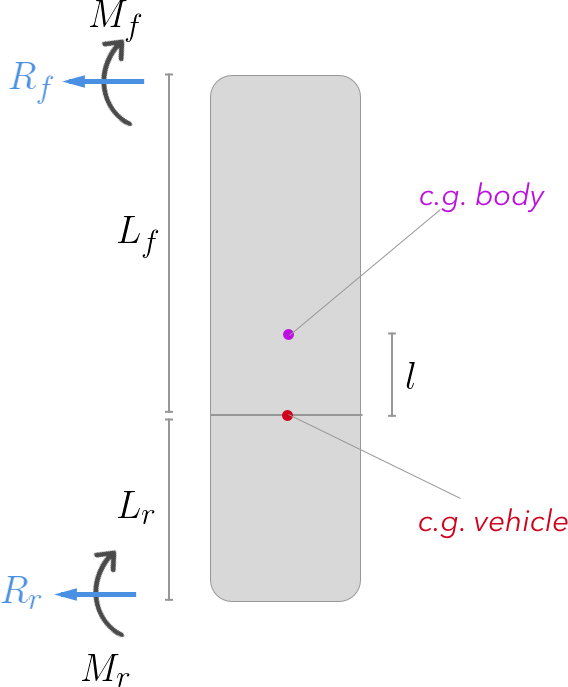
\includegraphics[width=1.1\linewidth]{figs/02/body_2}
	\caption{Free body diagram of the vehicle body}
	\label{body_1}
\end{marginfigure}
Using the relations derived above (from c.g) and simplifying:
\begin{equation}
m(\ddot{y}+V \dot{\psi}+\ddot{\theta}h \cos {\theta} - \theta^2 h \sin \theta)=F_{f}+F_{r}\]
\end{equation}
\begin{aligned}
M_{z}) \quad I_{o}\,\ddot{\psi}&=-M_{f}-M{\delta}\cos\beta-M_{r}+(L_{f}-l)R_{f}-(L_{r}+l)R_{r}\\
&=-M_{\delta}\cos\beta-2\,I_{wf,\psi}\ddot{\psi}-I_{wr,\psi}\ddot{\psi}-(I_{wr,\theta}-I_{wr,rot}w_{rot}\dot{\theta}+\\
&\quad +(L_{f}-l)\Big(F_{f}-2\,m_{wf}\big(\ddot{y}+V\dot{\psi}+h_{f}\n\ddot{\theta}\cos\theta-h_{f}\dot{\theta}^2\sin\theta+L_{f}\ddot{\psi}\big)\Big)-\\
&\quad-(L_{r}+l)\Big(F_{r}-m_{wr}\big(\ddot{y}+V\dot{\psi}+h_{r}\n\ddot{\theta}\cos\theta-h_{r}\dot{\theta}^2\sin\theta-L_{r}\ddot{\psi}\big)\Big)
\end{aligned}
\newpage
By means of the relations derived above and simplifying, the yaw dynamics equation is obtained:
\begin{equation}
I_{z}\,\ddot{\psi}=-(I_{wr,\theta}-I_{wr,rot})w_{rot}\dot{\theta}-M_{\delta}\cos\delta+L_{f}F_{f}-L_{r}L_{r}
\end{equation}
\begin{marginfigure}[-1cm]
	\includegraphics[width=0.9\linewidth]{figs/02/inertia}
	\caption{Front wheels axes and inertia notation}
	\label{body_1}
\end{marginfigure}
Thus the yaw dynamics have changed due to the gyroscopic terms from the rear wheel and the steering torque from the front wheels. The gyroscopic terms due to the front wheels do not appear directly in the vehicle yaw dynamic equations. Following the same procedure, the contribution to the tilt equations can be similarly derived.
\begin{itemize}
\begin{itemize}
\item With gyroscopic moments:\\$I_{z}\,\ddot{\psi}=-(I_{wr,\theta}-I_{wr,rot})w_{rot}\dot{\theta}-M_{\delta}\cos\delta+L_{f}F_{f}-L_{r}L_{r}$
\item Without gyroscopic moments: $I_{z}\,\ddot{\psi}=L_{f}F_{f}-L_{r}L_{r}$
\end{itemize}
\end{itemize}

\subsubsection{\textbf{Final Equations of Motion}}
\begin{eqnarray}
m\ddot{y}+mV \dot{\psi}+mh\ddot{\theta}\cos\theta - mh\theta^2\sin\theta=F_{f}+F_{r} \\
I_{z}\,\ddot{\psi}=L_{f}F_{f}-L_{r}L_{r}-(I_{wr,\theta}-I_{wr,rot})w_{rot}\dot{\theta}-M_{\delta}\cos\delta\\
I_{x} \ddot{\theta}=mgh\sin\theta - mh^2\ddot{\theta}\sin^2\theta - mh^2\dot{\theta}^2\cos\theta\sin\theta -\notag\\
-F_{f}h\cos\theta-F_{r}h\cos\theta +\textcolor{red}{2(I_{wf,\psi}-I_{wf,rot})w_{rot}(\dot{\psi}+\dot{\delta}\cos\beta)} + \textcolor{blue}{M_{t}}\\
2\,I_{wf,\psi}\ddot{\delta}=(M_{\delta}+M_{trail})\cos\beta-2(I_{wf,\theta}-I_{wf,rot})w_{rot}(\dot{\theta}-\dot{\delta}\sin\beta)
\end{eqnarray}

The part emphasized in red corresponds to the contribution of the gyroscopic terms to the tilting, whereas the blue part is the torque provided by the tilting motor.

\subsubsection{\textbf{Linearized Equations of Motion}}

The linearization is punctual, around the $\theta=0$ point. The longitudinal velocity is assumed constant, ($V_{x} = 8 m/s$), which is one of the most constraining hypotheses, and the angle of inclination is assumed to remain close to 0. To validate the use of this simplified model (dynamic simplifications and linearization), several velocities will be considered and the model will be linearized around several values.

The linearized equations using small angle approximations:
\begin{eqnarray}
m\ddot{y}+mV \dot{\psi}+mh\ddot{\theta}=F_{f}+F_{r} \\
I_{z}\,\ddot{\psi}=L_{f}F_{f}-L_{r}L_{r}-(I_{wr,\theta}-I_{wr,rot})w_{rot}\dot{\theta}-M_{\delta}\\
I_{x} \ddot{\theta}=mgh\theta -F_{f}h-F_{r}h + +2(I_{wf,\psi}-I_{wf,rot})w_{rot}(\dot{\psi}+\dot{\delta}) +M_{t}\\
2\,I_{wf,\psi}\ddot{\delta}=M_{\delta}+M_{trail}-2(I_{wf,\theta}-I_{wf,rot})w_{rot}\dot{\theta}
\end{eqnarray}
\newpage
\subsubsection{\textbf{Simplifying Hypotheses}}

The major simplifying hypotheses which led to the production of this bicycle model, which will serve as a support for the synthesis of control laws, are listed below: 
\begin{enumerate}\itemsep -7pt
\item Only 3 degrees of freedom: the lateral position $y$, and the tilt and yaw angles $\theta$,$\psi$. %and the steering angle $\delta$.
\item The longitudinal velocity $V_{x}$ is considered as an exogenous signal and not a system state variable. The model (2.22) is Linear Time-Variant (LTV), $V_{x}$ being a variant parameter.
\item The linearization is obtained around the angle of inclination $\theta=0$.
\item The vertical forces are assumed to be equal on both front wheels. 
\item The stiffness (slip coefficient) $C_{f}$ and the camber coefficient $\lambda_{f}$ are assumed to be constant.
\item The effect of the suspensions is neglected 
\item The wheels and the chassis are considered to be inclined to the same angle, and the point of contact of the tires do not change position during tilting.
\item The different mechanical parts moving within the vehicle, suspensions, links between different mechanical parts are not modeled.
\item The vehicle is assimilated to a mass located at the center of gravity which moves with the point of contact.
\end{enumerate}

\section{Literature Summary}

To sum up, in this chapter the literature regarding tilting vehicles has been reviewed. First, the  difference between active and passive systems was introduced, along with some examples of narrow three wheeler vehicles available to this day. In the field of active tilting systems, the distinction between the main control strategies was explained (DTC, STC and SDTC). Finally, using the literature, a dynamic model of the vehicle was derived.

The obtained linearized model is going to be the point of departure in the next chapter, regarding the control strategy.




\chapter{3. Control Strategy}

The objective of this chapter is to present the control strategy used in the PEV, based on the Direct Tilt Control (DTC). First, the lateral stability of the vehicle is studied, in order to understand the different strategies for lateral control. Then, the dynamic model is transformed into an space state model, much more easy to work with in control theory. Finally, the theory behind Linear Quadratic Regulator (LQR) and the Regulator Problem with Internal Stability (RPIS) is explained and the control gains are calculated.

\section{Stability Study}
\begin{marginfigure}[10cm]
	\includegraphics[width=1.2\linewidth]{figs/03/yz2}
	\caption{Forces acting on the center of gravity}
	\label{yz2}
\end{marginfigure}
\subsubsection{\textbf{Lateral Acceleration}}

The lateral acceleration $a_{lat}$ denotes the normal acceleration induced by the curvilinear motion of the vehicle, measured in the plane $XY$ at ground level at point D (Figure \ref{yz2}), and directed towards the center of rotation of the trajectory.
\[a_{lat}=\ddot{y}+V_{x}\dot{\psi}\]
Therefore, $a_{lat}$ is a function of the yaw rate (and hence the steering angle) and the longitudinal speed imposed by the driver. It is independent of the vertical position (angle of inclination) of the chassis.

\subsubsection{\textbf{Perceived Lateral Acceleration}}

In the frame reference $y',z'$, the acceleration at the point G decomposes into $a_{per}$ in the $y'$ direction and into $a_{z}$ in the $z'$ direction. The perceived lateral acceleration $a_{per}$ is the result of the accelerations at the center of gravity of the vehicle along the $y'$. 
\begin{equation}
a_{per}=a_{lat}\cos\theta+h\ddot{\theta}-g\sin\theta
\label{a_per}
\end{equation}
The objective for the control of lateral stabilization of the vehicle and the comfort of the driver will be to impose $a_{per}=0$. The vehicle is in lateral equilibrium if the perceived lateral acceleration is zero, i.e. $a_{per}=0$ (\textbf{sufficient condition for lateral stability})\cite[-2cm]{mourad:tel-00787310}.
\newpage
The fact that $a_{per}$ depends on $a_{lat}$ and $\theta$, implies that it depends on the trajectory, on the longitudinal velocity, and on the angle of inclination. However, the angle of inclination $\theta$ will be the key variable to ensure stability. We define by $\theta_{des}$ the desired position of $\theta$ which ensures $a_{per}=0$. 

\subsection{Lateral Stability}
\begin{marginfigure}[10cm]
	\includegraphics[width=1.2\linewidth]{figs/03/stability}
	\caption{Forces acting on the center of gravity}
	\label{stability}
\end{marginfigure}
In this section the dynamics of the vehicle are examined from the expression of $a_{per}$, in three distinct cases: 
\begin{enumerate}
\item \textbf{Vertical vehicle in straight path}

In this case $\theta=0$ and $a_{lat}=0$, therefore $a_{per}=0$ and the problem of lateral stability does not arise, except for the cases of rejection of lateral disturbance forces (i.e. side winds), or disturbances due to an asymmetric pavement on the left and right wheels. 

\item \textbf{Vertical vehicle in circular trajectory}

When the vehicle does not tilt (i.e $\theta=0$), then $a_{per}=a_{lat}$ (see equation (\ref{a_per})). If the intersection of the resultant accelerations at the center of gravity $G$ with the plane of the ground (point $x_G$) is outside the base of the vehicle, then it will be unstable. 
\[a_{G}=a_{lat}\,\vec{j} -g\,\vec{k}\]
On the contrary, if the point $x_G$ recalls inside the width of the vehicle, it will be stable. Then, the maximum lateral acceleration tolerated without inclination before the overturn is:
\begin{equation}
a_{lat-max}=\frac{gb}{2h}
\end{equation}
\\[-1cm]
\item \textbf{Inclined vehicle in circular trajectory}

When the vehicle is inclined at a certain angle $\theta$, its center of gravity has an offset, as well as the point $x_G$. The vehicle is stable as long as $x_G$ belongs to the segment $b$ and is, therefore, located between the two wheels of the vehicle. Let $\theta_n$ be the nominal inclination angle for which all accelerations in G are compensated, so that is solution of $a_{per}=0$. The computation of $\theta_n$ can seem complicated, but by considering the steady state (i.e. $\ddot{\theta}=\dot{\theta}=0$): $a_{per}=a_{lat}\cos\theta-g\sin\theta$. We then deduce the following expression:
\[\theta_{ref}=\theta_{n}=\tan^{-1}\Big(\frac{a_{lat}}{g}\Big)\]
This angle gives a resultant $a_{G}$ colinear with the axis $z'$ of the vehicle. Thus, the angle $\theta_{n}$ (solution of $a_{per}=0$) is an angle that guarantees the lateral stability of the vehicle.
\end{enumerate}

\subsection{Different strategies for lateral control}

The objective is to control the inclination of the vehicle so as to ensure its stability. In this way, the lateral stability of the vehicle and the comfort of passengers go hand in hand. From the sufficient condition of the stability explained above, the way to achieve this is by having null perceived acceleration at the center of gravity, $a_{per}=0$.

Two control strategies can be followed to reach this objective:

\begin{enumerate}
\item The stability is ensured by a \textbf{direct angular position control}, considering the angle of inclination of reference $\theta_{ref}$ ensuring $a_{per}=0$. This strategy has been widely adopted by researchers working on this issue. However, this strategy has some drawbacks: approximations have to be made to obtain at each moment the adapted reference angle, and its calculation potentially induces a \textbf{delay in the control}. 

\item An alternative solution is to \textbf{directly control the perceived acceleration}, and to pursue the $a_{per}=0$ objective. This is the strategy followed in this thesis. 
\end{enumerate}

Provided that the most readily available measurements on the vehicle are those provided by an inertial unit (IMU), the choice of direct control of $a_{per}$ was better adapted for these sensors.

\section{State of the Art for DTC, STC and SDTC systems}
Having defined the vehicle model, explained the problem of lateral stability, and calculated the various quantities concerned (lateral acceleration, perceived acceleration) it is now possible to clearly explain the work and results obtained by different researchers.

\begin{itemize}
\begin{itemize}
	\item \textbf{Hibbard Robbin \textit{et al.} 1996}\cite{hibbard1996twenty}, considered the problem of DTC vehicles and proposed to control the angle of inclination with the value of the reference calculated according to $\theta_{ref}$. The lateral acceleration was approximated by $V_{x}\dot{\psi}$, ignoring the dependence in $\ddot{y}$
\[\theta_{ref}=\tan^{-1}\Big(\frac{a_{lat}}{g}\Big)=\tan^{-1}\Big(\frac{\ddot{y}+V_{x}\dot{\psi}}{g}\Big)\approx\frac{V_{x}\dot{\psi}}{g}\] The control used for position feedback was a Proportional Derivative (PD) that has the error input on $\theta$, $e=\theta-\theta_{ref}$ with a feedforward function $a_{lat}=V_{x}\doc{\psi}$. The model used for regulator adjustment was reduced to the simplified transfer function between $\theta$ and $M_t$.

\item \textbf{So S. \textit{et al.}, 1997a}\cite{doi:10.1080/00423119708969321}, were interested in a system where STC and DTC actuated alternately, depending on the longitudinal speed of the vehicle.
\begin{itemize}
\item A filtered PD regulator was used for the DTC system: \[M_{t}=\Big(K_{p}+\frac{K_{d}}{\tau_{1}s+1}\Big)(\theta-\theta_{ref})\]
\item The STC strategy similarly used a PD with filtered derivative to calculate the appropriate steering angle.
\item The authors exploited the approximate relationship between $a_{lat}$ and $\delta$: $a_{lat}=\ddot{y}+V\dot{\psi}=(\dot{V}\,L_{r}\,\delta+V\,L_{r}\,\dot{\delta}+V^{2}\delta)/(L_{f}+L_{r})$. So $\theta_{ref-STC}=a_{lat}/g=f(\delta,\dot{\delta})$ and the control signal STC is written: \[\delta=\Big(G_{p}+\frac{G_{d}s}{\tau_{2}s+1}\Big)(\theta-\theta_{ref-STC})\]
\item The two controllers were first simulated separately, considering only the simplified transfer functions between $\delta$ and $\theta$ in STC and between the tilt torque $M_t$ and $\theta$ for DTC. The proposed results showed that the perceived acceleration in DTC was much greater than in STC, and that at the same time the steering angle was significantly modified in STC; 
\item Switching between STC and DTC systems was also considered, at speeds of $7.5 m/s$ and $8.5m/s$ depending on a hysteresis cycle. To circumvent the jump problems with respect to the static control value, the authors proposed a variable gain for the STC, which increased gradually to optimal value.
\end{itemize}

\item In their work, \textbf{So S. \textit{et al.}, (1997)}\cite{doi:10.1504/IJVD.1997.062071} replaced the PD controller with a PI for the DTC system to solve the static error problem and minimize discontinuity during STC-DTC switching. They added an additional feedback gain as a function of $\theta$ and $\dot{\theta}$. 

The validation of this work was very basic since no stability study was available, the lateral $a_{lat}$ and perceived $a_{per}$ accelerations were reconstructed by their approximate mathematical expressions and were not supposed to be directly measured; The simulations were carried out on a simplified model, linearized around $\theta=0$, considering the lateral and longitudinal dynamics.
\newpage
\item At the University of Minneapolis, the researchers addressed several aspects of lateral control of narrow tilting vehicles. In their work, \textbf{Piyabongkran D. \textit{et al.} (2004)}\cite{piyabongkarn2004active}, proposed three DTC control strategies in order to control the angle of inclination at $\theta_{ref}=\tan^{-1}(V\dot{\psi}/g)$, based on the linearized lateral model. 

\begin{itemize}
\item The first strategy was based on a Linear Quadratic Regulator (LQR) using a simplified model whose states only corresponded to $\theta$ and $\dot{\theta}$, hence ignoring the coupling with other important variables such as the yaw rate $\dot{\psi}$. A model of the driver was implemented to correct errors on the trajectory in simulation. 
\item The second strategy was based on the LQR control with a predictive aspect provided by the predictive estimation of the reference inclination angle, based on the knowledge of the future trajectory (i.e. on-board camera, GPS, etc. thus predicting the curvature of the road). The reference angle was obtained through a predictive command with a Receding Horizon Controller. 
\item The third proposed control strategy was nonlinear; it proceeded by inversion of the dynamics of the inclination angle (linearization by looping), which resulted in a double integrator dynamics $M_{t}=\ddot{\theta}$. A PID was then used such that $M_{t}=(K_{p}+K_{d}s+K_{i}/s)(\theta-\theta_{ref})$ 
\end{itemize}

The simulations showed that the nonlinear controller (strategy 3) was much more efficient than the LQ controller (strategy 2) in minimizing the tilt torque. The best performances were nevertheless obtained with the RCH controller (strategy 2), underlining the importance of the anticipation of the transient performance of the inclination control.

\item The SDTC commands were discussed by \textbf{Kidane, S. \textit{et al.} (2008), (2010})\cite{doi:10.1080/00423110701352987,5356230}. The authors proposed 3 DTC strategies, and 3 STC strategies, in order to find the methodology ensuring the best switching in SDTC. 

The \textbf{DTC strategies} were all based on a PD controller, but differed in the expression of the reference $\theta_{ref}$ chosen:
\begin{enumerate}
\item $\theta_{ref}=\frac{V\dot{\psi}}{g}=\frac{V^2}{gR}$
\item $\theta_{ref}=\frac{\ddot{y}+V\dot{\psi}}{g}-\frac{2(I_{wheel rot}\,w\,\dot{\psi}/(hm)}{g}$
\item $\theta_{ref}=k_{s}(\delta_{driver})$
\end{enumerate}

The first expression is the most simplified; it neglects the term of lateral slip $\ddot{y}$, which leads to a significant increase in the transient torque. The second expression is more rigorous and the term $2(I_{wheel rot}\,w\,\dot{\psi}/(mgh)$, which takes into account the gyroscopic moments at the level of the wheels, leads to a zero static error, but it is difficult to calculate. Finally, to circumvent the problem of contradictory STC and DTC control signals, the authors retained the third expression (i.e. $\theta_{des}=k_{s}(\delta_{driver})$), although it is very approximate and does not optimize the torque required in transient situations. 

The \textbf{STC strategies} also used a PD controller, with an additional term $\delta_{ss}$, which allowed a steering angle equal to that desired by the driver to be obtained in steady state: $\delta=K_{p}(\theta-\theta_{ref})+K_d{\dot{\theta}-\dot{\theta}_{ref})+\delta_{ss}$. The three STC strategies differed in their choice of $\delta_{ss}$:

\begin{enumerate}
\item The most complete proposed expression uses the value of unmeasured and therefore inaccessible variables.
\item An alternative expression performs the rewriting of expression 1. as a function of $\theta_{ref}$ and parameters to be estimated.
\item The last strategy replaces $\delta_{ss}$ by an integral term on the deviation $(\theta-\theta_{ref})$. This is the solution chosen for the SDTC command.
\end{enumerate}

\item The \textbf{SDTC controller} was then made up of two independent PIDs; one controller generated the motor torque $M_{t}$, and the second the steering angle $\delta$ applied to the wheels. $V_o$ and $V_f$ were two threshold values, $V_{o}<V_{f}$ for the longitudinal velocity. For $V<V_{o}$, the DTC system is active; for $V>V_{f}$, the STC system takes over; For $V_{o}<V<V_{f}$ a function dependent on $V$ shared the control between DTC and STC. 

The controller was validated in simulation and experimentally by \textbf{Kidane S. \textit{et al.}, 2010}\cite{5356230}. The results were acceptable, but the perceived lateral acceleration was not given, and no stability study was proposed. On the other hand, the proposed SDTC controller did not explicitly optimize the energy required for implementing this strategy.
\newpage

\item In the Netherlands, \textbf{Carver Europe} developed a three-wheel recliner called Carver. This vehicle was equipped with a Dynamic Vehicle Control system that used the DTC and STC strategies. The publications relating to this system remain evasive, probably due to the confidentiality of the project. However, several patents are filed separately concerning the use of the steering angle in the tilt controller (CR Van Den Brink \textit{et al.}, 1999)\cite[-3cm]{van1999realization}, the simultaneous action of the STC and DTC systems (CR Van Den Brink And Kroonen, 2004)\cite{van1997dynamic}.

\item At the \textbf{University of Bath}, researchers worked on the \textbf{Clever} project: a three-wheeled vehicle, in which only the chassis and front wheel were tilted. This vehicle was equipped with a DTC system, operating with hydraulic actuators. In their work, Berote \textit{et al.}, (2008)\cite{bath15090} the authors focused on the analysis of the Clever dynamics, emphasizing the importance of rear wheel steering to limit the risk of over-turning of the vehicle. The authors also evoked the advantage of having the axis of rotation of the vehicle inclined (and not horizontal), which affects the inertia of the inclination movement. The DTC controller remained very basic: a PD to control the angle of inclination. 

\end{itemize}
\end{itemize}

\newpage
\section{DTC: Summary of Difficulties and Solutions}

In this section the problems of DTC control are identified, and solutions are proposed to improve the performance of the controller.

\subsection{Difficulties related to DTC} 

DTC strategies are generally based on a pursue of the angle of inclination $\theta$, such that $\theta\rightarrow\theta_{ref}$, where $\theta_{ref}$ is given by the expression  $\theta_{ref}=\tan^{-1}(a_{lat}/g)$ or even more simplified or approximate versions which have been described in detail in the previous section (i.e. $\theta_{ref}=V_{x}\dot{\psi}/g$, or $\theta_{ref}=k_{s}(\delta_{driver})$, etc.). The weak points of these strategies can be summarized as follows:
\begin{enumerate}
\item \textbf{High torque from the actuator on the transient phase}: the calculation of $\theta_{ref}$ from the measurement of lateral acceleration $a_{lat}$ or yaw angle $\dot{\psi}$, induces an \textbf{intrinsic delay}: the actuator is only activated after the detection of the lateral acceleration through the accelerometer. The inclination torque must therefore compensate for the lateral acceleration already present, which inclines the vehicle towards the outside of the curve before being able to incline it in the opposite direction with the actuator. 

\begin{figure*}[!h]
	\includegraphics[width=1.0\linewidth]{figs/03/torque}
	\caption{Transitional phase of the vehicle approaching a turn: increasing $a_{lat}$, inclining the vehicle outside the turn and requiring a greater $M_t$}
	\label{torque}
\end{figure*}

The longer the $M_t$ reaction, the greater the lateral acceleration, and the greater the required tilt torque. When other sensors that allow the trajectory prediction are installed on the vehicle (camera), this anticipation makes it possible to reduce the tilting torque significantly (Piyabongkran D. and Al., 2004)\cite[0cm]{piyabongkarn2004active}. In addition, the lateral acceleration ($a_{lat}=\ddot{y}+V\dot{\psi}\cos\beta$) is proportional to the speed. Thus, the higher the speed, the greater the lateral acceleration and the greater the torque $M_t$ required.
\newpage
\item \textbf{Static error}: Given the way in which the reference is calculated,  $\theta=\theta_{ref}$ does not mean that $a_{per}$ is strictly null. Consequently, the actuator must permanently supply a non-zero torque to maintain the inclination of the vehicle at $\theta_{ref}$.
\end{enumerate}
\subsection{Proposed solutions} 

The two main solutions to improve the operation of the DTC systems are: A) Using the steering angle input from the driver as a regulator and B) Directly controlling the perceived lateral acceleration.
\begin{enumerate}
\item \textbf{Reduction of the actuator torque in DTC}

When driving of a motorcycle, the rider tilts it as soon as the turn begins, before the appearance of the lateral acceleration. Consequently the effort required for the inclination is relatively small; and this is also the case for a vehicle whose path is known in advance. It is, thus, essential to initiate the inclination as soon as possible. 

The first measurable signal containing information about the near trajectory is the \textbf{angle (or even the torque) of steering}. This signal must be used in order to initiate the inclination of the vehicle before the perception of lateral acceleration. %This will be an essential part of the strategy followed in this thesis.

The steering angle is considered as a \textbf{disturbance} which induces an increase in the perceived lateral acceleration, such as to destabilize the vehicle. In order to be able to use this signal in the controller, a control methodology is chosen to be able to take into account this knowledge of the environment. 

\item \textbf{Cancellation of the static error and improvement of the DTC performance}

The lateral stability is obtained by the appropriate inclination of the vehicle. It is therefore intuitive to seek to control the angle of inclination $\theta\rightarrow\theta_{ref}$ by calculating the necessary torque to achieve an inclination coherent with the terminal objective: $a_{per}=0$. To reduce the problem of the approximation and to reduce the risks of instability ($\theta_{ref}$ is deduced from the state variables) the \textbf{direct control of the perceived lateral acceleration} $a_{per}$ is proposed.\cite{6315042}

Therefore, the objective variable is now the $a_{per}=0$ rather than $\theta=\theta_{ref}$. In addition, in order to ensure the robust asymptotic cancellation of the static error, the integral of $a_{per}$ ($a_{per}^{I}$) will be taken into account. This approach is much more interesting since $a_{per}$ is measured by the inertial motion unit (IMU).
\end{enumerate}
\newpage
\section{Design of the DTC Controller}
\subsection{Dynamic Model}
In the previous chapter, the linearized dynamic model was obtained:
\begin{eqnarray}
\label{dynamic_model_1}
m\ddot{y}+mV \dot{\psi}+mh\ddot{\theta}=F_{f}+F_{r} \\
I_{z}\,\ddot{\psi}=L_{f}F_{f}-L_{r}L_{r}-(I_{wr,\theta}-I_{wr,rot})w_{rot}\dot{\theta}-M_{\delta}\\
I_{x} \ddot{\theta}=mgh\theta -F_{f}h-F_{r}h + +2(I_{wf,\psi}-I_{wf,rot})w_{rot}(\dot{\psi}+\dot{\delta}) +M_{t}\\
2\,I_{wf,\psi}\ddot{\delta}=M_{\delta}+M_{trail}-2(I_{wf,\theta}-I_{wf,rot})w_{rot}\dot{\theta}
\label{dynamic_model_2}
\end{eqnarray}
\[F_{f}=2 C_{f}\Big(\delta - \frac{\dot{y}+L_{f} \dot{\psi}}{V} \Big) + 2 \lambda_{f} \theta\]
\[F_{r}=C_{r}\Big(- \frac{\dot{y}-L_{r} \dot{\psi}}{V} \Big) +\lambda_{r} \theta\]

The inputs to this model are the steering angle $\delta$ and the tilting torque $M_{t}$.

\subsection{Methodological Approach}
The general idea consists in formalizing the problem through the construction of a generic model, called standard, allowing the reformulation of the problem of control in an optimization problem $H_{2}$\cite[-2cm]{Zhou:1996:ROC:225507}. This model $P(S)$ is structured and consists of the aggregation of:
\begin{itemize}
\begin{itemize}
\item \textbf{Plant}: A model of the system to be monitored, displaying disturbance and control signals and well as the output variables to be controlled.
\item \textbf{Disturbance}: A model of the environment of the system to be controlled, generating the exogenous signals such as perturbations and setpoints.
\item \textbf{Output}: A model of the quantities to be regulated, including weights constituting adjustment coefficients.
\end{itemize}
\end{itemize}
\begin{marginfigure}[-4.5cm]
	\includegraphics[width=1.2\linewidth]{figs/03/standard}
	\caption{Standard Problem}
	\label{standard}
\end{marginfigure}

The associated $H_{2}$ is considered in the generic form, which consists in determining $K_{s}$ stabilizing the process model and minimizing: $\lVert P(s)\,K(s) \rVert _{2}$

\subsection{State Space Model}
The obtained model of the form described by equations (\ref{dynamic_model_1}-\ref{dynamic_model_2}) is reduced to its controllable and observable part which has 4 states $(\dot{y},\dot{\psi},\theta,\dot{\theta})$.
The Linear Parameter Variant (LTV) model is parameterized by the longitudinal speed $V$ of the vehicle:
%\begin{equation}
%\begin{cases}\dot{x}(t)=A(V)\,x(t)+B\,u(t)\\ y(t)=C\,x(t)+D\,u(t)\end{cases}
%\end{equation}
\begin{equation}
\begin{cases}\dot{x}=A\,x+B_{u}\,u+B_{d}\,d\\ y=C\,x+D_{u}\,u+D_{d}\,d\end{cases}
\end{equation}

with $x^{T}=\begin{bmatrix}
\dot{y} & \dot{\psi} & \theta & \dot{\theta}
\end{bmatrix}^{T} \in \Re^4$, $u=M_{t}$ and $d=\delta$

$A=\begin{bmatrix} 
\frac{1}{V}\big(-\frac{a}{m}-\frac{h^{2}a}{I_{x}}\big) & \frac{1}{V}\big(-\frac{b}{m}-\frac{h^{2}b}{I_{x}}\big)-V & (2\lambda_{f}+\lambda_{r})\big(\frac{1}{m}+\frac{h^2}{I_{x}}\big)-\frac{mgh^2}{I_{x}} & 0\\
-\frac{b}{V\,I_{z}} & -\frac{2C_{f}L_{f}^{2}+C_{r}L_{r}^{2}}{V\,I_{z}} & \frac{2\lambda_{f}L_{f}-\lambda_{r}L_{r}}{I_{z}} & 0\\
0 & 0 & 0 & 1\\
\frac{h\,a}{V\,I_{x}} & \frac{h\,b}{V\,I_{x}} & \frac{mgh-h(2\lambda_{f}+\lambda_{r}}{I_{x}} & 0
\end{bmatrix}
$\\[10pt]
$B_{d}=B_{\delta}=\begin{bmatrix} 2C_{f}\big(\frac{1}{m}+\frac{h^2}{I_{x}} & \frac{2C_{f}L_{f}}{I_{z}} & 0 & -\frac{2C_{f}h}{I_{x}} \end{bmatrix}^{T}$,\\[10pt]
$B_{u}=B_{M_{t}}=\begin{bmatrix} -\frac{h}{I_{x}} & 0 & 0 & \frac{1}{I_{x}} \end{bmatrix}^{T}$, $a=2\,C_{f}+C_{r}$, $b=2\,C_{f}L_{f}-C_{r}L_{r}$

The model becomes an Linear Time Invariant (LTI) model when a constant longitudinal velocity $V$ is considered. The vector $x$ denotes the states , $y$ the measured the outputs, $u$ the control input and $d$ is considered as a disturbing exogenous signal\cite{kCraig}.

\subsection{Estimation of $\dot{y}$}
The PEV will include a Inertial Measurement Unit (IMU), which will provide the state values $\theta$, $\dot{\theta}$, and $\dot{\psi}$, but not $\dot{y}$. The IMU will also give the value for the perceived lateral acceleration $a_{per}$. Note that this measure was not used in the previous strategy, nor in the classical strategy of controlling $\theta$ such that $\theta=\theta_{des}$ steering angle $\delta$ and its derivative $\dot{\delta}$ will be measured.

The state signal $\dot{y}$ can be estimated from the measured signals: $y_{p}=\begin{bmatrix}
\dot{\psi} & \theta & \dot{\theta} & a_{per} \end{bmatrix}^{T}$, according to:\\[8pt]
\begin{aligned}
\hat{\dot{y}}=(a_{11}+ha_{41})^{-1}\Big[a_{per}-(a_{12}+ha_{42}+V_{x})\dot{\psi}-(a_{13}+ha_{43}-g)\theta \\- (a_{14}+ha_{44})\dot{\theta}-(b_{\delta 1}+hb_{\delta 4})\delta-(b_{u1}+hb_{u4})M_{t}\Big]
\end{aligned}
\\[8pt] where terms $a_{ij}$, $b_{\delta i}$ and $b_{ui}$ are coefficients of matrices $A$, $B_{\delta}$ and $B_{u}$ respectively.

\subsection{Expressing $a_{per}$ as function of $x$}
Lateral stability of the vehicle is obtained when the sum of lateral forces and torques at its center of gravity is zero ($a_{per}=0$). 

$\hspace{1.5cm} a_{per}=a_{lat}\cos\theta+h\ddot{\theta}-g\sin\theta$\quad with  \quad $a_{lat}=\ddot{y}+V\,\dot{\psi}$

The $a_{per}$ is a measured signal, but is not part of the state vector. Using small angle approximations, it can be expressed as a function of the state vector as follows:
\[a_{per}\approx\ddot{y}+V\,\dot{\psi}+h\ddot{\theta}-g\theta=a_{per}^{lin}\]
\[a_{per}^{lin}=\begin{bmatrix} 0 & V & -g & 0 \end{bmatrix} x + \begin{bmatrix} 1 & 0 & 0 & h \end{bmatrix} \dot{x}=G_{1}\,x+G_{2}\,\dot{x}\]

Replacing $\dot{x}$ by $A\,x+B_{u}\,u+B_{d}\,d$ leads to:
\[a_{per}^{lin}=G_{1}\,x+G_{2}(A\,x+B_{u}\,u+B_{d}\,d)=G\,x+H_{u}\,u+H_{d}\,d\]
with $G=G_{1}+G_{2}\,A$, $H_{u}=G_{2}\,B_{u}$ and $H_{d}=G_{2}\,B_{d}$. The output vector is defined as $y=\begin{bmatrix} a_{per} & \dot{\psi} & \theta & \dot{\theta} & \delta \end{bmatrix}^{T}$ Therefore:

$\hspace{2cm} C=\begin{bmatrix}
G \\ \begin{bmatrix} 0_{3x1} I_{3} \end{bmatrix} \\ 0_{1x4} 
\end{bmatrix}$, $D_{u}=\begin{bmatrix}
H_{u} \\ 0_{4x1}
\end{bmatrix}$, $D_{d}=\begin{bmatrix}
H_{d} \\ 0_{3x1} \\ 1
\end{bmatrix}$

\subsection{Regulator Problem with Internal Stability \cite{6315042}}

The fundamental control objective to ensure the lateral stability is to solve the regulation problem $a_{per}=0$. The problem formulation is recast as a standard regulator problem with internal stability (RPIS) where $\delta$ is considered as a disturbance, and its effect on the perceived lateral acceleration $a_{per}$ should be canceled by the tilt torque $M_{t}$. 

\begin{figure}[!h]
	\includegraphics[width=0.95\linewidth]{figs/03/control}
	\caption{Control diagram: Feedforward and feedback loops}
	\label{control}
\end{figure}

\textbf{Plant Model}
\begin{equation}
\begin{cases}\dot{x}=A\,x+B_{u}\,u+B_{d}\,d\\ y=C\,x+D_{u}\,u+D_{d}\,d\\ z=G\,x+H_{u}\,u+H_{d}\,d\end{cases}
\end{equation}
with $G=\begin{bmatrix}
-{a}/{V\,m} & -{b}/{V\,m} & (2\lambda_{f}+\lambda_{r})/m - g & 0
\end{bmatrix} \\[6pt] H_{u}=0, H_{d}={2C_{f}}/{m}$

\textbf{Disturbance Model} 
\begin{equation}
\begin{cases}\dot{x_{e}}=A_{e}\,x+B_{e}\,w\\ d=C_{e}\,x_{e}\end{cases}
\end{equation}
with $x_{e}^{T}=\begin{bmatrix}
\delta & \dot{\delta}
\end{bmatrix}^{T}$, $C_{e}=\begin{bmatrix}
1 & 0
\end{bmatrix} $, $A_{e}=\begin{bmatrix}
0 & 1 \\ -\tau\alpha & -(\tau +\alpha) 
\end{bmatrix}$, $B_{e}=\begin{bmatrix}
0 \\ \beta
\end{bmatrix}$

where $w$ is an impulse signal, $\alpha$, $\tau$ and $\beta$ determine the time constants and amplitude of the $2^{nd}$ order signal. This model is critical to obtain good performances in transient phases, while the feedback takes care of the static ones and guarantees robust regulation.

\textbf{Standard Model}\\[6pt]
\[\begin{bmatrix} \dot{x} \\ \dot{x_{e}} \end{bmatrix} = \begin{bmatrix}
A & B_{d}\,C_{e} \\ 0 & A_{e}\end{bmatrix}\begin{bmatrix} x \\ x_{e} \end{bmatrix} +\begin{bmatrix} B_{u} \\ 0 \end{bmatrix} u + \begin{bmatrix}0 \\ B_{e} \end{bmatrix} w\]

\[e=z=\begin{bmatrix}G & H_{d}\,C_{e}\end{bmatrix}\begin{bmatrix}x \\ x_{e}\end{bmatrix} + H_{u}\,u\]

\[y=\begin{bmatrix}x \\ x_{e}\end{bmatrix}=\begin{bmatrix}
\dot{y} & \dot{\psi} & \theta & \dot{\theta} & \delta & \dot{\delta}\end{bmatrix}^{T}\]

\textbf{Solution for RPIS}

Assuming that the plant model is stabilizable, a solution for the RPIS problem exists in the feedback form if the unique solution ($T_{a},F_{a}$) of the occultation equations exists:
\begin{eqnarray}
-A\,T_{a}+T_{a}\,A_{e}+B_{d}\,C_{e}=-B_{u}\,F_{a} \\
-G\,T_{a}+H_{d}\,C_{e}=H_{u}\,F_{a}
\end{eqnarray}

If $\exists\, T_{a}, F_{a} \rightarrow u_{ref}=-F_{a}\,x_{e}$ and $x_{ref}=-T_{a}\,x_{e}$ is the unique reference trajectory for the plant model that satisfies the control objective $e=a_{per}=0$. Therefore this trajectory satisfies the dynamic of the system:
\begin{equation}
\begin{cases}\dot{x}_{ref}=A\,x_{ref}+B_{u}\,u_{ref}+B_{d}\,d\\ z_{ref}=G\,x_{ref}+H_{u}\,u_{ref}+H_{d}\,d\end{cases}
\label{sylvester}
\end{equation}
Defining $(\tilde{u},\,\tilde{x},\,e)=(u-u_{ref},\,x-x_{ref},\,z-z_{ref})$ the difference between the actual and desired values of the current control input, states and controlled output.

The first step is to compute the feedback gain $K$, designed such that $\tilde{u}=-K\tilde{x}$ guarantees $\tilde{x}\rightarrow 0$ and $e\rightarrow 0$ (stabilization of the plant). The second step a feedforward gain is designed in order for $(u,x)$ to follow the reference trajectory $u_{ref},x_{ref}$ in an optimal way.

\textbf{Feedback Gains}

For the calculation of the feedback gains, the Linear Quadratic Regulator (LQR)\cite{lec5}\cite{rob3}\cite{Wonham:1614618} has been chosen based on the good robustness properties, few tuning parameters and the explicit minimization of the energy of control signals required to follow the reference.

The LQR consists on finding the state feedback $\tilde{u}=-K\tilde{x}$ that minimizes the criteria:
\[J_{LQR}=\int_{0}^{\infty}{\big(z^{T}\,Q\,z + u^{T}\,R\,u \big) dt}=\int_{0}^{\infty}{\big(x^{T}\,Q_{x}\,x + u^{T}\,R\,u + 2 x^{T}\,N_{xu}\,u\big) dt}\]
The weighting matrices $Q$ and $R$ must be positive and will balance the minimization of the state vector or the control signal.
\[Q_{x}=G^{T}\,Q\,G\]
\[R_{u}=H_{u}^{T}\,Q\,H_{u} + R\]
\[N_{ux}=G^{T}\,Q\,H_{u}\]
The solution is given by:
\[K=-R_{u}^{-1}\,B_{u}^{T}\,P\]
Where $P$ is the unique solution of the Riccati equation applied to the plant model:
\[A^{T}\,P+P\,A-P\,B_{u}\,R_{u}^{-1}\,B_{u}^{T}\,P+Q_{x}=0\]

\textbf{Feedforward Gains}

Solving the Sylvester equations in (\ref{sylvester}) and using the feedback gains $K$, the feedforward gain is calculated as $K_{d}=F_{a}+K\,T_{a}$.

\begin{aligned}
\tilde{u}=-K\tilde{x} \quad \rightarrow \quad & u-u_{ref}=-K\,(x-x_{ref}) \\[6pt] & u + F_{a}\,x_{e}=-K(x+T_{a}\,x_{e} \\
& u=-K\,x -(F_{a}+K\,T_{a})x_{e}=-K\,x-K_{d}\,x_{e}
\end{aligned}

\subsection{Extended model with the integral of $a_{per}$: $a_{per}^_{I}$}
In order to avoid any static error, the integrated value of the lateral perceived acceleration will be controlled, and its value will be added to the state vector. In fact, it is unavoidable to have some model errors due to parameters uncertainty, neglected dynamics or linearization of the model.

The equation to add to the model is very simple: 
\[\dot{a_{per}^_{I}}=a_{per}=G\,x+H_{u}\,u+H_{d}\,d\]
The augmented state is then $x_{i}=\begin{bmatrix} \dot{y} & \dot{\psi} & \theta & \dot{\theta} & a_{per}^_{I} \end{bmatrix}$, and the new system:
\begin{equation}
\begin{cases}\dot{x_{i}}=A\,x_{i}+B_{iu}\,u+B_{id}\,d\\ z=a_{per}^_{I}}=G_{i}\,x_{i}+H_{iu}\,u+H_{id}\,d\end{cases}
\end{equation}

\[A_{i}=\begin{bmatrix} A & 0_{4x1} \\ G & 0{1x1} \end{bmatrix}, \quad B_{iu}=\begin{bmatrix} B_{u} \\ H_{u} \end{bmatrix}, \quad B_{id}=\begin{bmatrix} B_{d} \\ H_{d} \end{bmatrix}\]
\[G_{i}=\begin{bmatrix} 0 & 0 & 0 & 0 & 1 \end{bmatrix}, \quad H_{iu}=0, \quad H_{id}=0\]

\textbf{Extended Standard Model}\\[6pt]
\[\begin{bmatrix} \dot{x_i} \\ \dot{x_{e}} \end{bmatrix} = \begin{bmatrix}
A_{i} & B_{id}\,C_{e} \\ 0_{2x5} & A_{e}\end{bmatrix}\begin{bmatrix} x_{i} \\ x_{e} \end{bmatrix} +\begin{bmatrix} B_{iu} \\ 0_{2x1} \end{bmatrix} u + \begin{bmatrix}0_{2x1} \\ B_{e} \end{bmatrix} w\]\\[6pt]
\[e=z=a_{per}^_{I}}=\begin{bmatrix}G_{i} & H_{id}\,C_{e}\end{bmatrix}\begin{bmatrix}x_{i} \\ x_{e}\end{bmatrix} + H_{iu}\,u\]\
\[y=\begin{bmatrix}x \\ x_{e}\end{bmatrix}=\begin{bmatrix}
\dot{y} & \dot{\psi} & \theta & \dot{\theta} & a_{per}^_{I} & \delta & \dot{\delta}\end{bmatrix}^{T}\]

\textbf{Feedback Gains}

The Linear Quadratic Regulator is adapted to the extended model: 
\[J_{LQR}=\int_{0}^{\infty}{\big(z^{T}\,Q\,z + u^{T}\,R\,u \big) dt}=\int_{0}^{\infty}{\big(x^{T}\,Q_{x}\,x + u^{T}\,R\,u + 2 x^{T}\,N_{xu}\,u\big) dt}\]
\[Q_{x}=G_{i}^{T}\,Q\,G_{i} \hspace{1cm} R_{u}=H_{iu}^{T}\,Q\,H_{iu} + R \hspace{1cm} N_{ux}=G_{i}^{T}\,Q\,H_{iu}\]
The solution is given by:
\[K=-R_{u}^{-1}\,B_{iu}^{T}\,P\]
Where $P$ is the unique solution of the Riccati equation applied to the plant model:
\[A_{i}^{T}\,P+P\,A_{i}-P\,B_{iu}\,R_{u}^{-1}\,B_{iu}^{T}\,P+Q_{x}=0\]

\textbf{Feedforward Gains}

The Sylvester equations in (\ref{sylvester}) need to be adapted to the new model:
\begin{eqnarray}
-A_{i}\,T_{a}+T_{a}\,A_{e}+B_{id}\,C_{e}=-B_{iu}\,F_{a} \\
-G_{i}\,T_{a}+H_{id}\,C_{e}=H_{iu}\,F_{a}
\end{eqnarray}
By solving these equations and using the feedback gains $K$, the feedforward gain is calculated as $K_{d}=F_{a}+K\,T_{a}$.

\textbf{Simple Method Gains Calculation}

A straightforward way of calculating the gains is to solve the Riccati and the Sylvester equations as it is indicated in (Friedland, Chapter 9.6)\cite{control-system-design} book:

	-- Riccati eq: $\quad M_{1}\,A_{i} + A_{i}^{T}\,M_{1} - M_{1}\,B_{iu}\,R_{u}^{-1}B_{iu}^{T}M_{1} + Q_{x}=0$

	-- Slyvester eq: $\quad M_{2}\,A_{e}+(A_{i}^{T}-M_{1}\,B_{iu}\,R_{u}^{-1}\,B_{iu}^{T})M_{2}+M_{1}\,B_{id}\,C_{e}=0$

Then, the gains can be easily calculated:
\begin{itemize}
\begin{itemize}
\item Feedback gains: $K=R_{u}^{-1}\,B_{iu}^{T}\,M_{1}$
\item Feedforward gains: $K_{d}=R_{u}^{-1}\,B_{iu}^{T}\,M_{2}$
\end{itemize}
\end{itemize}

\subsection{Derivation of the Gains}

As was discussed previously, the state variable $\dot{y}$ is not measured and can only be estimated as:

\begin{aligned}
\hat{\dot{y}}=(a_{11}+ha_{41})^{-1}\Big[a_{per}-(a_{12}+ha_{42}+V_{x})\dot{\psi}-(a_{13}+ha_{43}-g)\theta \\- (a_{14}+ha_{44})\dot{\theta}-(b_{\delta 1}+hb_{\delta 4})\delta-(b_{u1}+hb_{u4})M_{t}\Big]
\end{aligned}

To calculate the real gains on the controller, a simple but tedious derivation has to be carry out:
\[u=-K\,x_{i}-K_{e}\,x_{e}\]
\[u=-K_{\dot{y}}\,\dot{y}-K_{\dot{\psi}}\,\dot{\psi}-K_{\theta}\,\theta-K_{\dot{\theta}}\,\dot{\theta}-K_{a_{per}^{I}}\,a_{per}^{I}-K_{\delta}\,\delta-K_{\dot{\delta}}\,\dot{\delta}\]
\newpage
\begin{aligned}
u&=-\frac{K_{\dot{y}}}{a_{11}+ha_{41}}\,a_{per} - \Big(K_{\dot{\psi}}-K_{\dot{y}}\frac{a_{12}+ha_{42}+V_{x}}{a_{11}+ha_{41}}\Big)\dot{\psi} -  \Big(K_{\theta}-K_{\dot{y}}\frac{a_{13}+ha_{43}-g}{a_{11}+ha_{41}}\Big)\theta - \Big(K_{\dot{\theta}}-K_{\dot{y}}\frac{a_{14}+ha_{44}}{a_{11}+ha_{41}}\Big)\dot{\theta} - \\[10pt] &\quad -  K_{a_{per}^{I}}\,a_{per}^{I} - \Big(K_{\delta}-K_{\dot{y}}\frac{b_{\delta 1}+hb_{\delta 4}}{a_{11}+ha_{41}}\Big)\delta-K_{\dot{\delta}}\,\dot{\delta}-K_{\dot{y}}\,\frac{b_{u1}+hb_{u4}}{a_{11}+ha_{41}}\,u
\end{aligned}
\\

\begin{aligned}
u=\frac{1}{1+K_{\dot{y}}\,\frac{b_{u1}+hb_{u4}}{a_{11}+ha_{41}}}\Big[&-\frac{K_{\dot{y}}}{a_{11}+ha_{41}}\,a_{per} - \Big(K_{\dot{\psi}}-K_{\dot{y}}\frac{a_{12}+ha_{42}+V_{x}}{a_{11}+ha_{41}}\Big)\dot{\psi} - \Big(K_{\theta}-K_{\dot{y}}\frac{a_{13}+ha_{43}-g}{a_{11}+ha_{41}}\Big)\theta - \\[10pt] & - \Big(K_{\dot{\theta}}-K_{\dot{y}}\frac{a_{14}+ha_{44}}{a_{11}+ha_{41}}\Big)\dot{\theta} -  K_{a_{per}^{I}}\,a_{per}^{I} - \Big(K_{\delta}-K_{\dot{y}}\frac{b_{\delta 1}+hb_{\delta 4}}{a_{11}+ha_{41}}\Big)\delta-K_{\dot{\delta}}\,\dot{\delta}\Big]
\end{aligned}
\\

\begin{aligned}
u=\frac{1}{a_{11}+ha_{41}+K_{\dot{y}}\,(b_{u1}+hb_{u4})}\Big[&-K_{\dot{y}}\,a_{per} - \big[K_{\dot{\psi}}(a_{11}+ha_{41})-K_{\dot{y}}(a_{12}+ha_{42}+V_{x})\big]\dot{\psi} - \\[8pt] & - \big[K_{\theta}(a_{11}+ha_{41})-K_{\dot{y}}(a_{13}+ha_{43}-g)\big]\theta - \\[8pt] & - \big[K_{\dot{\theta}}(a_{11}+ha_{41})-K_{\dot{y}}(a_{14}+ha_{44})\big]\dot{\theta} -  K_{a_{per}^{I}}(a_{11}+ha_{41})\,a_{per}^{I} - \\[8pt] & - \big[K_{\delta}(a_{11}+ha_{41})-K_{\dot{y}}(b_{\delta 1}+hb_{\delta 4})\big]\delta-K_{\dot{\delta}}(a_{11}+ha_{41})\,\dot{\delta}\Big]
\end{aligned}
\\

With this estimation all the signals are measured and have a gain:
\begin{eqnarray}
K_{a_{per}}^{'}=\frac{K_{\dot{y}}}{a_{11}+ha_{41}+K_{\dot{y}}\,(b_{u1}+hb_{u4})} \\[10pt]
K_{\dot{\psi}}^{'}=\frac{K_{\dot{\psi}}(a_{11}+ha_{41})-K_{\dot{y}}(a_{12}+ha_{42}+V_{x})}{a_{11}+ha_{41}+K_{\dot{y}}\,(b_{u1}+hb_{u4})} \\[10pt]
K_{\theta}^{'}=\frac{K_{\theta}(a_{11}+ha_{41})-K_{\dot{y}}(a_{13}+ha_{43}-g)}{a_{11}+ha_{41}+K_{\dot{y}}\,(b_{u1}+hb_{u4})} \\[10pt]
K_{\dot{\theta}}^{'}=\frac{K_{\dot{\theta}}(a_{11}+ha_{41})-K_{\dot{y}}(a_{14}+ha_{44})}{a_{11}+ha_{41}+K_{\dot{y}}\,(b_{u1}+hb_{u4})} \\[10pt]
K_{a_{per}^{I}}^{'}=\frac{K_{a_{per}^{I}}(a_{11}+ha_{41})}{a_{11}+ha_{41}+K_{\dot{y}}\,(b_{u1}+hb_{u4})} \\[10pt]
K_{\delta}^{'}=\frac{K_{\delta}(a_{11}+ha_{41})-K_{\dot{y}}(b_{\delta 1}+hb_{\delta 4})}{a_{11}+ha_{41}+K_{\dot{y}}\,(b_{u1}+hb_{u4})} \\[10pt]
K_{\dot{\delta}}^{'}=\frac{K_{\dot{\delta}}(a_{11}+ha_{41})}{a_{11}+ha_{41}+K_{\dot{y}}\,(b_{u1}+hb_{u4})}
\end{eqnarray}
\[K^{'}=\begin{bmatrix}
K_{a_{per}}^{'} & K_{\dot{\psi}}^{'} & K_{\theta}^{'} & K_{\dot{\theta}}^{'} & K_{a_{per}^{I}}^{'} & K_{\delta}^{'} & K_{\dot{\delta}}^{'}
\end{bmatrix} \]
\newpage
\subsection{Gain Scheduled Controller}
The previous regulator was synthesized by considering a constant value of the longitudinal speed $V_{x}$. But the state space model is LPV and the matrices $A$ and $C$ depend on $V$ or $1/V$. Thus, the proposed controller is not valid for the whole speed range. In this section, a controller that depends on the longitudinal speed of the vehicle is proposed. 

The approach adopted is pragmatic, and proceeds by interpolation of the LTI regulators obtained for a discrete set of longitudinal speeds. It thus guarantees a good performance at every operating point. Stability guarantees will also be provided by a posteriori analysis. 

The first step is the observation of the gain variation of this regulator as a function of velocity for $V \in {2,3,...18}\,m/s $. A regulator is synthesized for each value of $V$ and the variation of the gains can be approximated by a function of the form:
\[K(V)=K_{c}+K_{V}\,V+K_{1/V)\V\]
Dependent on $V$ and $1/V$, with $K_{c}$, $K_{V}$ and $K_{1/V}$ the constants to be identified. These values can be easily deduced from the least squares resolution of the following system of equations:
\[
\underbrace{\begin{pmatrix}
1 & V_{1} & 1/V_{1} \\ 1 & V_{2} & 1/V_{2} \\ ... & ... & ... \\ 1 & V_{17} & 1/V_{17} \\
\end{pmatrix}}_{M} 
\begin{pmatrix} K_{c} \\ K_{V} \\ K_{1/V} \end{pmatrix}=
\underbrace{\begin{pmatrix} K_{V_{1}}^{'} \\K_{V_{2}}^{'} \\ ... \\ K_{V_{17}}^{'} \end{pmatrix}}_{K_{M}}
\Rightarrow
\begin{pmatrix} K_{c} \\ K_{V} \\ K_{1/V} \end{pmatrix}=(M^{T}\,M)^{-1}\,M^{T}\,K_{M}\]

\newpage
\section{Control Strategy Summary}
In this chapter the control strategy has been completely derived and developed. The process of calculating the gains can be resumed in few steps:
\begin{enumerate}
\item To obtain or measure the \textbf{parameters to complete the dynamic model}. This includes the vehicle and the wheels variables: 

$\hspace{2cm} m \enspace L_{f} \enspace L_{r} \enspace I_{x} \enspace I_{z} \enspace C_{f} \enspace C_{r} \enspace \lambda_{f} \enspace \lambda_{r} \enspace ...$.

\item To suppose a \textbf{constant $V$ for the model}, so that $V \in {2,3,...18}\,m/s $

\item To generate the \textbf{matrices of the state space} model:

$\hspace{1.5cm} A \enspace B_{u} \enspace B_{d} \enspace C \enspace D_{u} \enspace D_{d} \enspace G \enspace H_{u} \enspace H_{d} \enspace A_{e} \enspace B_{e} \enspace C_{e} \enspace ...$

\item \textbf{Feedback gains}: To solve the Riccati equation for the selected model and calculate the gains: 

$\hspace{1.5cm} M_{1}\,A_{i} + A_{i}^{T}\,M_{1} - M_{1}\,B_{iu}\,R_{u}^{-1}B_{iu}^{T}M_{1} + Q_{x}=0$

$\hspace{3.5cm} K=R_{u}^{-1}\,B_{iu}^{T}\,M_{1}$

\item \textbf{Feedforward gains}: To solve the Slyvester equation for the selected model and calculate the gains: 

$\hspace{1cm}M_{2}\,A_{e}+(A_{i}^{T}-M_{1}\,B_{iu}\,R_{u}^{-1}\,B_{iu}^{T})M_{2}+M_{1}\,B_{id}\,C_{e}=0$

$\hspace{3.5cm} K_{d}=R_{u}^{-1}\,B_{iu}^{T}\,M_{2}$

\item \textbf{Gain Scheduling}: To repeat the steps 2 to 5 with all the speed range and calculate the constants $K_{c}$, $K_{V}$ and $K_{1/V}$  with:

$\hspace{2.5cm}\begin{pmatrix} K_{c} \\ K_{V} \\ K_{1/V} \end{pmatrix}=(M^{T}\,M)^{-1}\,M^{T}\,K_{M}$

\end{enumerate}

\chapter{4. Small Scale Prototype}

As a first step towards the design and fabrication of a tilting PEV, an small scale prototype was built. In this chapter the design and fabrication process regarding this small vehicle, also called \textbf{miniPEV}, will be explained.

\section{Concept - Deploy or Die}

In sight of the Media Lab's motto '\textbf{deploy or die}'\cite{deploydie}, the objective of this thesis would be to deploy a real scale vehicle with a tilting mechanism. However, the process to reach that goal needs a lot of iterations, try and errors, and a small scale prototype is a good starting point.

\begin{marginfigure}
	\includegraphics[width=1.1\linewidth]{figs/04/deploy_die}
	\caption{Evolution of the philosophy of innovation at the Media Lab}
\end{marginfigure}

A small moving tilting prototype  -- \textbf{miniPEV}-- is helpful in a lot of different ways. It is much easier to show your ideas and the story behind narrow tilting vehicles to people who are not familiarized  with this kind of vehicles. As a matter of fact, the miniPEV was shown in the Fall Member Event at the Media Lab. The feedback received from the sponsors, students, and people from the MIT community was really helpful to understand better the problem and its opportunities in the mobility sector.

The miniPEV\cite{miniPEV} is a simple tilting 'toy' car make out of wood. It is approximately one quarter of the scale of the PEV, but as a concept, it represents all the features that a full scale vehicle has.
It is propulsed by a DC motor, and two servomotors move the two front steering wheels and the tilting mechanism. It also has a battery to power all the electronics and the motors. In order to simulate the same inputs to the control system, a Inertial Measurement Unit (IMU) was also installed and used to tilt the vehicle in the curves. The details regarding the components will be explained later in this chapter.



\newpage
\section{Design}

The design on the miniPEV was based on a previous small prototype by Michael Lin, head of the PEV project at Changing Places group. In order to fabricate the prototype as fast as possible, the miniPEV was built with plywood sheets of $3mm$, that were cut in the laser cutting machine. Then, gluing the layers together gives result to the final 3D model. In this way, the prototype is fabricated very fast and the possibilities of making changes is high as well.

The model is composed of different parts. In the rear part there is a seat, and the wheel is propulsed from the hub. The electronics and the battery are placed in the center, with the aim of keeping the model as balanced as possible and having a low center of gravity. Due to the limitations of power, this design decision was critical for the proper motion of the model. The front part consist of two steered wheels with their steering system and a suspension that allows the tilting of the vehicle.

\section{Tilting Mechanisms}

This section focuses on explaining the tilting mechanism chosen for the miniPEV, as an introduction to the more detailed simulations carried out for the full scale PEV. 

The different tilting mechanisms that previous tilting vehicles have used can be summarized in two categories:
\begin{enumerate}
\item \textbf{Hydraulic actuators}: located in the suspension or in a fixed part of the vehicle, they can incline the vehicle by extending one of the two actuators. The size and power provided by these actuators exceed the requirements and the space available in the PEV, as well as in the miniPEV. This strategy has been used in car-like vehicles rather than in bike-like vehicles.

\item \textbf{Rotary motor}: being much compact, a high torque motor can supply the necessary $M_{t}$ to lean the vehicle when necessary. Here the possibilities of actuating the vehicle expand, but the design remains basic. Attached to the motor there is a arm that connects to the suspension arms, meaning that the rotation of the motor reduces and enlargers the distance from the body to the suspension, hence tilting the vehicle and the wheels. This second option is the one that is going to be explored next, due to the different possibilities that comprises.
\end{enumerate}

\newpage
\textbf{Rotary Motor Tilting Mechanisms}

If a rotary motor is used, the first question that arises is: What part of the vehicle would we like to tilt? The answer falls on selecting the parts that we do not want to lean. In a tadpole vehicle like PEV with 2 front wheels and 1 rear wheel (the contrary will be a delta vehicle - 1F2R), the part that can maintain vertical by itself is the front suspension and the wheels. In this way, we could separate the whole front part from the rest of the frame (handle bar, cover, seat, rear wheel...), implying that the tilting part would be the body of the vehicle. This is indeed the alternative \textbf{A} (Figure \ref{design_tilting}):

\begin{figure}[h!]
	\includegraphics[width=1.0\linewidth]{figs/04/Picture2}
	\caption{Tilting mechanisms alternatives based on the suspension and body independence}
	\label{design_tilting}
\end{figure}

\textcolor{Bittersweet}{A: Separate body from suspension}

In this case the front suspension does not lean, it maintains as if the vehicle did not have a tilting degree of freedom and the wheels maintain vertical as well. Therefore, the suspension keeps its design objective: to absorb the vibration and the bumps reactions coming from the irregular profile of the ground. The current design of the suspension could be used for this tilting PEV. 

On the other side, the junction part between the two parts supposes a high risk point, since all the forces in the vehicle will be concentrated in that point. In addition, it would require to re-design the steering mechanism, since there is a mismatch between the two parts.
\begin{marginfigure}
	\includegraphics[width=1.2\linewidth]{figs/04/a_option}
	\caption{Design proposal in the joint with option A}
\end{marginfigure}
\begin{itemize}
\begin{itemize}\itemsep -10pt
    \item[$\textcolor{Green}{\surd}$] Suspension does not lean, wheels maintain vertical
    \item[$\textcolor{Green}{\surd}$] Suspension used for vibration absorption
    \item[$\textcolor{Green}{\surd}$] No changes in suspension design
\end{itemize}
\end{itemize}

\begin{itemize}
\begin{itemize}\itemsep -10pt
    \item[$\textcolor{Red}{\times}$] Robust design required, risk point
    \item[$\textcolor{Red}{\times}$] Concentration of forces in the joint
    \item[$\textcolor{Red}{\times}$] Steering re-design
\end{itemize}
\end{itemize}

\newpage
\textcolor{RubineRed}{B: Body moves with suspension}

When the vehicle leans with the suspension, then the wheels also tilt (the camber changes) and there is no risk point since all the frame parts are joint together. Apart from small changes, the steering system can be maintained, which is a advantage. However, this alternative also gives rise to other issues. Leaning the wheels can imply an instability in the vehicle, since some tires are not designed to be tilted an elevate angle. There are also a great deal of actuation strategies, which can be difficult to choose from. 

Nevertheless, the main drawback of this design is that the suspension is not anymore independent from the leaning on the vehicle. This implies that the suspension shock absorbers need to change their position and that the motor actuation cannot conflict with the motion of the suspension due to vibrations or bumps. This issue is really challenging, and in this project we were not able to design a front suspension that separated the suspension motion from the tilting motion. We will sacrifice the absence of the suspension for the sake of reaching to a new concept of tilted tricycle.
\begin{itemize}
\begin{itemize}\itemsep -10pt
    \item[$\textcolor{Green}{\surd}$] Suspension and wheels do lean
    \item[$\textcolor{Green}{\surd}$] Robust design: no risk point
    \item[$\textcolor{Green}{\surd}$] Keep steering design
\end{itemize}
\end{itemize}

\begin{itemize}
\begin{itemize}\itemsep -10pt
    \item[$\textcolor{Red}{\times}$] Suspension not independent from leaning
    \item[$\textcolor{Red}{\times}$] Multiple actuation strategies
    \item[$\textcolor{Red}{\times}$] Stability of the wheels
\end{itemize}
\end{itemize}

To understand the different tilting suspensions, the program Autodesk ForceEffect software was used as a first approach. The suspension was modelled in a 2D plane, with only 1 degree of freedom (which accounts for the leaning of the suspension). 

\begin{figure}[h!]
	\includegraphics[width=1.0\linewidth]{figs/04/b}
	\caption{Front suspension model in 2D}
\end{figure}

\newpage
The main parts and the links between them are, from left to right:

\begin{itemize}
\begin{itemize}\itemsep -10pt
	\item \textit{Wheel (Left)}: Co-linear bars $\overline{AC}$ and $\overline{BC}$. Point A is in contact with the ground by an articulation. Distance $\overline{AC}$ represents the radius of the front wheel.
	\item \textit{Kingpin (Left)}: Co-linear bars $\overline{DE}$ and $\overline{DF}$. It is inclined by the kingpin angle. 
	\item \textit{Hub (Left)}: $\overline{CD}$ bar, welded to the left wheel and the kingpin.
	\item \textit{Upper/Lower Suspension Arms}: bar $\overline{FG}$/$\overline{EH}$ articulated in both sides.
	\item \textit{Body}: it represents the frame of the vehicle, where the driver will be sitting. Four-sided solid body $GHIJ$.
	\item \textit{Rotation Point}: $Q$ is the point from which the motor will actuate.
	\item \textit{Tilting Mechanism}: Bars $\overline{QR}$ and $\overline{RT}$/$\overline{RS}$.
	\item \textit{Wheel (Right)}: Co-linear bars $\overline{QO}$ and $\overline{OR}$. Point Q is in contact with the ground by a slider.
\end{itemize}
\end{itemize}

With this basic model in mind, the four studied alternatives can be summarized as follows. A more detailed analysis of the front suspension will be explained in the next chapter as well.

\begin{itemize}
\begin{itemize}
	\item \textbf{B.1 Rotating point on top of body + linkage (shock absorbers) to upper arms}
	
	\begin{figure*}[h!]
		\includegraphics[width=1.1\linewidth]{figs/04/b_1}
		\caption{$B_{1}$ option}
	\end{figure*}
	The tilting mechanism consists of three elements. The arm $\overline{QR}$ is actuated by the motor, and the two remaining bars ($\overline{RU}$ and $\overline{RV}$) are connected to the upper arms. This is the bar system used in the miniPEV. It is a very simple mechanism, but in terms of geometry, requires an angle of \textbf{45 degrees} between the $\overline{QR}$ and $\overline{RU}$ bars in order to get maximum torque on the suspension bars. The rotation point $Q$ is constrained to be on top of the body, and considering the length of the $\overline{QR}$ bar, the space requirement is high.
	\newpage
	\item \textbf{B.2 Rotating point below body + linkage (shock absorbers) to lower arms}
	
	\begin{figure*}[h!]
		\includegraphics[width=1.1\linewidth]{figs/04/b_2}
		\caption{$B_{2}$ option}
	\end{figure*}
	This strategy is very similar to the B.1, but the motor is located below the body. This can create problems with the motor touching the ground in some circumstances, something that should be avoided. If compared to the previous option, this alternative is not recommended. 
		
		\item \textbf{B.3 Rotating point inside body + horizontal shock absorbers to lower arms}
	
	\begin{figure*}[h!]
		\includegraphics[width=1.1\linewidth]{figs/04/b_3}
		\caption{$B_{3}$ option}
	\end{figure*}
	Using a rotary motor and a rack-pinion system, the rotational motion can be transformed into a linear (horizontal) motion, thus changing the distance between the lower suspension arms and tilting the vehicle.
	
	\newpage
	\item \textbf{B.4 Rotating point inside body + gearbox to lower arm}
	
	By means of a gearbox, the torque coming from the motor is increased, as the suspension arms are actuated art the same time. The simplicity and freedom to choose the reduction ratio were the main reasons why this option was designed, fabricated and assembled in the full scale PEV.
	\begin{figure*}[h!]
		\includegraphics[width=1.1\linewidth]{figs/04/b_4}
		\caption{$B_{4}$ option}
	\end{figure*}
\end{itemize}
\end{itemize}
As has already been stated, the miniPEV will have a tilting mechanism similar to the option B.1 whereas the full scale PEV will be designed following the B.4 design. 

\subsection{First Sketches}

At first, some drawings were made to illustrate the model in three dimensions.
In Figure \ref{sketch_1}, the tilt actuator and the arms with the shock absorbers activate the tilting on the trike. The suspension is constituted by a 4-bar mechanism; the simplest bar system that allows a tilting motion.
\begin{figure}[h!]
	\includegraphics[width=0.95\linewidth]{figs/04/Imagen5}
	\caption{Sketch of tilting mechanism}
	\label{sketch_1}
\end{figure}

The front and rear views of the suspension (Figure \ref{sketch_2}) clarify the 4-bar mechanism mentioned previously. When the vehicle runs into a bump, the shock absorbers in the affected side compress, thus minimizing the vibrations that reach to the driver. In addition, the suspension allows the tilting of the vehicle an angle $\theta$, which will be limited by the geometry, but should not exceed 30 degrees.
\begin{figure*}[h!]
	\includegraphics[width=1.0\linewidth]{figs/04/Imagen6}
	\caption{Sketches with response to bump and tilting}
	\label{sketch_2}
\end{figure*}

\\In Figure \ref{sketch_3} more detailed drawings of the suspension have been included.
\begin{figure*}[h!]
	\includegraphics[width=1.0\linewidth]{figs/04/Imagen10}
	\caption{Detailed sketches of the tilting suspension}	
	\label{sketch_3}
\end{figure*}

\newpage
\section{Components}

In this section the components of the miniPEV and their main characteristics are reviewed.

\begin{figure}[h!]
	\includegraphics[width=0.95\linewidth]{figs/04/CreamBoxtemp0150}
	\caption{miniPEV explosion render}
\end{figure}
%\begin{figure}[h!]
%	\includegraphics[width=1.0\linewidth]{figs/04/CreamBoxtemp0210}
%	\caption{miniPEV render}
%\end{figure}
\begin{itemize}
\begin{itemize}
	\item Wood Frame and Wheels
	
	Taking as example other previous wood models from the group, the vehicle was designed in Solidworks. The body is made of 3mm plywood sheets, and the rear wheel is slightly bigger than the front ones. Using the laser cutting machine, the body, the wheels, and the rest of the parts were fabricated quite fast. The fact that the model was made out of plywood brought along a lot of issues during the motion of the vehicle. This type of prototypes are not usually designed to move, but to remain static instead. In any case, there was a lot of effort in reducing the friction between the moving parts (wheels and steering system).
	
	\begin{figure}[h!]
		\includegraphics[width=1.0\linewidth]{figs/04/11}
		\caption{Lateral view of the render}
	\end{figure}
	
	\newpage
	\item Rear DC Motor
	
	The rear motor is a Pololu DC motor of 12V and a gearbox integrated. The gearbox fits perfectly in this application, providing a high output torque to be able to move the vehicle. The torque increase is about 50:1, and the motor's small size allows it to hide in the frame.
	\begin{marginfigure}[-2cm]
		\includegraphics[width=0.75\linewidth]{figs/04/pololu}
		\caption{Rear DC Motor, Pololu 50:1 Micro Metal Gearmotor }
	\end{marginfigure}
	
	Controlling a DC motor with Arduino requires a transistor and a diode. The small DC motor is likely to use more power than an Arduino digital output can handle directly (50mA). Connecting the motor straight to an Arduino pin would damage the Arduino. Tha is why a small transistor like the PN2222 needs to be used as a switch, that uses just a little current from the Arduino digital output to control the much bigger current of the motor. 

There is also a diode connected across the connections of the motor. Since diodes only allow electricity to flow in one direction, when to motor turns off the diode protect the Arduino and the transistor from a negative spike of voltage. The diode protects against this, by shorting out any such reverse current from the motor.
	
	\item Steering and Tilting	
	
	The steering servo motor is located vertically in the left side of the vehicle, and has two bars linked to the hubs of the front wheels. The tilting motor is laying on top of the body, horizontally, and has a glass arm attached to the output shaft. This glass piece is connected to the shock absorbers that are attached to the upper suspension arms. 
	
	The tilting servo motor is slightly more powerful than the steering motor, since the force requirement for the tilting motion is higher than for turning the wheels.
	
	\begin{marginfigure}[-13cm]
		\includegraphics[width=0.75\linewidth]{figs/04/servo}
		\caption{Servo Motor MG90}
	\end{marginfigure}
	
	\begin{marginfigure}[-4cm]
		\includegraphics[width=0.85\linewidth]{figs/04/55758}
		\caption{Miniature shock absorbers MA 35 to MA 900}
	\end{marginfigure}
	
	\begin{figure}[h!]
		\includegraphics[width=0.95\linewidth]{figs/04/22}
		\caption{Front view of the render}
	\end{figure}

	\item Electronics
	
	The \textbf{Arduino UNO} is the board responsible for receiving the inputs from the sensors and controlling the output to the three motors. The board and all the components are powered by a 12V DC battery (\textbf{Energizer XP8000}). The election of the 12V is due to the rear motor input voltage. The rest of the components (servo motors, bluetooth module and IMU) only require 5V, voltage that the Arduino board can provide from one of its pins. All these electronic components are placed in a mini breadboard.
	
	The chosen IMU both for the miniPEV and for the PEV is the \textbf{Adafruit BNO055 Absolute Orientation Sensor}, with 9DOF (accelerometer, gyroscope and magnetometer). It is connected through the I2C connection (SDA and SCL pins) to the board. The measurements from this sensor are the angular velocity along the vertical axis $Z$ (\textbf{yaw rate} $\dot{\psi}$) and the \textbf{linear acceleration} in the forward direction $a_{x}$, which will be integrated to estimate the longitudinal speed of the vehicle.
	
	As a matter of fact, the use of this Inertial Measurement Unit is quite easy, since the libraries to get the data have been already developed. Nevertheless, there are some steps that need to be followed in order to configure the sensor in the first place (this will be intensively explained in the next chapter).
	
	\hfill
	
	\begin{marginfigure}
		\caption{Electronic Components}
	\end{marginfigure}
	\begin{figure}[!h]
		\minipage{0.5\textwidth}%
			\includegraphics[width=1.0\linewidth]{figs/04/uno}
			\captionof{a)}{ Arduino UNO board}
		\endminipage
		\minipage{0.5\textwidth}
			\includegraphics[width=1.0\linewidth]{figs/04/MiniBreadBoard}
		    \captionof{b)}{ Mini breadboard}
		\endminipage\hfill
	\end{figure}
	
	\hfill
	
	\begin{figure}[!h]
		\minipage{0.5\textwidth}
			\includegraphics[width=1.0\linewidth]{figs/04/battery}
		  	\captionof{c)}{ Energizer XP8000 battery}
		\endminipage\hfill
		\minipage{0.5\textwidth}
			\includegraphics[width=1.0\linewidth]{figs/04/bno055}
		    \captionof{d)}{ BNO055 9DOF IMU}
		\endminipage\hfill
	\end{figure}

	\newpage
	Finally, in order to remotely connect with the board and control the vehicle, a Bluetooth HC05 module was installed. This module was connected through serial connection to the Arduino. An Android application was the installed in the phone to activate different functions (forward, left, right...). The wiring diagram is represented as follows:
	
	\begin{figure*}[h!]
		\includegraphics[width=0.9\linewidth]{figs/04/miniPEV_bb}
		\caption{miniPEV Electronics Schematic}
	\end{figure*}

	
\end{itemize}
\end{itemize}
\hfill

\section{Final Model and Results}

The final model is illustrated in the Figures \ref{minipev1} and \ref{minipev2}. The tilting servo motor is controlled to satisfy in every moment that $\theta=\theta_{ref}$, with \[\theta_{ref}=\frac{V\,\dot{\psi}}{g}\] This expression of the roll angle reference was introduced in the previous chapter and is based on a very simple model that combines the bicycle and the inverted pendulum dynamics (Figure \ref{miniPEV_model}).

\begin{marginfigure}[-3cm]
	\includegraphics[width=0.75\linewidth]{figs/04/Imagen2}
	\caption{miniPEV simple model to obtain the $\theta_{ref}$}
	\label{miniPEV_model}
\end{marginfigure}

\begin{figure}[h!]
	\includegraphics[width=1.0\linewidth]{figs/04/IMG0943}
	\caption{Lateral view of the miniPEV}
	\label{minipev1}
\end{figure}

\begin{figure}[h!]
	\includegraphics[width=1.0\linewidth]{figs/04/IMG0956}
	\caption{Front view of the miniPEV}
	\label{minipev2}
\end{figure}

\newpage
The value for the angular velocity (yaw rate) $\dot{\psi}$ is obtained from the gyroscope sensor measurement. However, there is no direct information about the longitudinal velocity of the vehicle.  That is why the linear acceleration in the forward direction $a_{x}$ is integrated, thus estimating the velocity $V$.

A strategy in two steps was carried out to filter and integrate the linear acceleration signal. First, a Kalman filter was used and, in second place, a more manual filtering was implemented. In order to validate the integration algorithms, some live tests were made. These test samples were obtained from the Media Lab elevator, going up and down several times.

\newpage
\textbf{Kalman Filter}

A Kalman filter is an optimal estimation algorithm used to estimate states of a system from indirect and uncertain measurements. The most simple Kalman filter has some variables: $x$ for the filtered value, $q$ for the process noise, $r$ for the sensor noise, $p$ for the estimated error and $k$ for the Kalman Gain. 

The filter is applied with each measurement and initialized with the process noise $q$, the sensor noise $r$, the initial estimated error $p$ and the initial value $x=0$. The initial value for $p$ is not very important since it is adjusted during the process. It must be just high enough to narrow down. The filter can be summed up in two simple steps:

\begin{itemize}
\begin{itemize}
	\item Predict
	
	The current state $x_{k}$ is estimated from the previous state $x_{k-1}$ and the estimated error $p$ increases by the inherent process noise $q$.\[x_{k}=x_{k-1}, \quad p=p+q\]
	\item Measurement Update
	
	The kalman gain $k$ balances the relevance of the current observation $z_{k}$ and the previous state $\hat{x}_{k-1}$. It is the ratio of the estimated error $p$ and the noise coming from the sensor $r$. \[k=\frac{p}{p+r}, \quad \hat{x}_{k}=\hat{x}_{k-1}+k(z_{k}-\hat{x}_{k-1})\] When the gain is 0, the current observation has no effect on the updated value, whereas if its value is 1 the previous state does not have an influence.

\end{itemize}
\end{itemize}

After filtering the acceleration $a_x$ with $x_{0}=0 \quad p=1\quad q=0.01\quad r=0.15\quad$, the velocity is integrated with the \textbf{trapezoidal rule of numerical integration}: \[\hat{v}_{k}=\hat{v}_{k-1}+(a_{k}+a_{k-1})\frac{\Delta t}{2}\] The issue with this strategy is the shift of the velocity origin due to the noise in the acceleration and the error in the time interval. These errors accumulate during the ups and downs in the elevator, and incorrectly gives non-zero values of the velocity.

There is an extended Kalman filter that accounts for this shift issue, but is designed to correct the possible shifts in the sensors signals, that is, to fix any possible deviation in the signal coming from the IMU. In this case, we are trying to deal with a numerical integration, not a shift in the signal from the IMU. Therefore, this path is not applicable to this case.

The Kalman filter is perfect for filtering the noise from the accelerometer, but it is not enough to give a good estimation of the velocity when integrating the filtered acceleration. 

\begin{figure}[h!]
	\includegraphics[width=1.0\linewidth]{figs/04/acceleration/1}
	\caption{Kalman filtering to elevator test}
\end{figure}
\begin{figure}[h!]
	\includegraphics[width=1.0\linewidth]{figs/04/acceleration/2}
	\caption{Elevator velocity estimation with trapezoidal rule}
\end{figure}

\textbf{Integration Shift}

In order to fix the accumulative error in the integration of the acceleration, a very simple algorithm was implemented. This algorithm just corrected the shift by estimating the slope ($m$) of the error during an early sample. 

\begin{itemize}
\begin{itemize}
	\item Trapezoidal
	\[\hat{v}_{k}=\hat{v}_{k-1}+(a_{k}+a_{k-1})\frac{\Delta t}{2}\]

	\item Corrected:
	\[\hat{v}_{k}=\hat{v}_{k-1}+(a_{k}+a_{k-1})\frac{\Delta t}{2}-m\,\Delta t\]
\end{itemize}
\end{itemize}
\newpage

\begin{figure}[h!]
	\includegraphics[width=1.0\linewidth]{figs/04/acceleration/3}
	\caption{Sample from the elevator}
\end{figure}
\begin{figure}[h!]
	\includegraphics[width=1.0\linewidth]{figs/04/acceleration/4}
	\caption{Acceleration, and integration with trapezoidal rule and a corrected estimation}
\end{figure}

After calibrating this algorithm, a final test was carried out in the elevator, giving good results (Figure \ref{filtered}).

\begin{figure}[h!]
	\includegraphics[width=1.0\linewidth]{figs/04/acceleration/6}
	\caption{Final test in the elevator}
	\label{filtered}
\end{figure}


\section{Chapter Conclusions}

The design and fabrication of the miniPEV supposed the first step in this project, and has been really useful for understanding the possible problems that could rise in a tilting vehicle of bigger dimensions. Sometimes looking at a prototype for five minutes is much more productive than thinking about its design and making hundreds of sketches. It also was useful to explain to the Changing Places group and other labmates the ideas that were being developed. 

\begin{marginfigure}
	\includegraphics[width=1.0\linewidth]{figs/04/sponsors_fall2}
	\caption{miniPEV stand at the Media Lab Members Event Fall 2016}
\end{marginfigure}

In the technical side, there were some challenges. First, the estimation of the longitudinal speed of the vehicle required several tests and some time going up and down in the Media Lab elevator (which was kind of fun). The results of these test were useful for the integration of other variables in the full scale vehicle.

Regarding the tilting control, the delay between the input from the driver and the action from the motor was evident. This agrees with the studies mentioned previously in the literature review.

Overall, the vehicle satisfactorily performed as expected, and the tilting worked perfectly, even though the motor-actuated glass part was larger than in the initial design. In the next chapter the real scale PEV will be presented.

\begin{figure}[h!]
	\includegraphics[width=1.0\linewidth]{figs/04/remote}
	\caption{Remote control from the phone to the miniPEV via Bluetooth}
	%\label{filtered}
\end{figure}


\chapter{5. Real Scale Prototype}

Once the dynamic model and the control strategy have been studied, the design and fabrication of the tilting PEV will be explained in this chapter. The frame of this vehicle was recycled from another previous PEV version, and will be the departure point for this new prototype. In this chapter we will cover the processes to design and fabricate all the parts in the vehicle, (front suspension, tilting and steering mechanisms, rear motor, handle bar, batteries, electronic components...)

\section{Front Suspension Design}
The first step is to design the front suspension of the vehicle. The suspension arms will continue to form a four bar mechanism as were in the miniPEV. In this case, before designing any mechanical component and jumping to the CAD software, some kinematic and dynamic simulations were carried out. These simulations had several goals in mind.
\begin{enumerate}\itemsep -10pt
\item Understand the motion of the tilting suspension depending on its geometry.
\item Maintain the wheels as vertical as possible during the leaning of the body.
\item Minimize the required torque from the tilting motor. 
\end{enumerate}
The simulations were developed in MATLAB, following a similar structure to the functions introduced in the book by A. Avello\cite{iturriagagoitia2014teoria}. The analysis starts by defining a model of elements that are linked together by different types of joints. This model is then translated into a set of equations $\Phi$ that define the constraints of the system. Whichever the motion of the mechanism, it must obey these equations. 

\newpage
The kinematic simulations require to solve three problems (position, velocity and acceleration) in that order. Then the dynamic simulation makes use of the results from the kinematic analysis, giving an estimation of the forces and reactions in the system.

\subsection{Model Schematic}

The first step to a mechanical analysis is to generate a model of elements that represent the system. In this case, the front suspension is abstracted into a 2D model of bars. 

The process of designing the model is very simple. The user introduces the length of the bars, then the coordinates of all points are calculated from a fixed frame reference and based on those bar lengths. Finally, the estimated mass of each bar is introduced, and all possible external forces are applied as well. For example, the weight of the driver is simulated as a 80kg weight located in a point near to the center of gravity of the vehicle.

\begin{figure}
	\includegraphics[width=1.0\linewidth]{figs/05/sim/1}
	\caption{Simulated Model}
	\label{model_schematic}
\end{figure}

Based on the Autodesk ForceEffect model designed previously, the suspension model was implemented in MATLAB. It has 20 points -- 3 of them fixed, A, B, C -- that define the bars. There are only three types of links in the model: articulations, weld and slider. 

The constraint equations that define this model can be summarized in these types (the examples have been taken from the model in Figure \ref{model_schematic}):

\marginnote{$x_{i}$ is the x coordinate of the point i\\
$y_{i}$ is the y coordinate of the point i\\
$L_{a\,b}$ is the length of the bar $a$-$b$}
\begin{itemize}
\begin{itemize}
\item Bar $\hspace{1.25cm}(x_{1}-x_{3})^{2}+(y_{1}-y_{3})^{2}-L_{1\,3}^{2}=0$

\item Triangle  \begin{aligned}
(x_{1}-x_{2})^{2}+(y_{1}-y_{2})^{2}-L_{1\,2}^{2}=0\\
\hspace{0.5cm}(x_{1}-x_{9})^{2}+(y_{1}-y_{9})^{2}-L_{1\,9}^{2}=0\\
\hspace{0.5cm}(x_{2}-x_{9})^{2}+(y_{2}-y_{9})^{2}-L_{2\,9}^{2}=0
\end{aligned}

\item Welded \begin{aligned}
(x_{6}-x_{7})(x_{4}-x_{7})+(y_{6}-y_{7})(y_{4}-y_{7})-L_{6\,7}L_{4\,7}\cos(90)=0\\
\hspace{0.5cm}(x_{6}-x_{7})(y_{4}-y_{7})-(y_{6}-y_{7})(x_{4}-x_{7})-L_{6\,7}L_{4\,7}\sin(90)=0
\end{aligned}

\item Slider $\hspace{0.75cm}(x_{6}-x_{B})(y_{B}-y_{C})-(y_{6}-y_{B})(x_{B}-x_{C})=0$
\end{itemize}
\end{itemize}

Each of these constraint equations is denoted as $\Phi(\vec{g},t)$, since depend in the vector of the coordinates $\vec{g}$ and the time $t$.

In Figure \ref{model_schematic} only 16 moving and 3 fixed points have been represented. The model will be completed with the introduction of the tilting actuation and the driver model. In total there will be 20 moving points and 3 relative coordinates (angles), which make a total of \textbf{43 unknown coordinates}.
\[\vec{g}=\begin{bmatrix} x_{1}\quad y_{1}\quad x_{2}\quad ... \quad x_{20}\quad y_{20} \quad \theta \quad \gamma \quad \phi \end{bmatrix}_{43x1}\]
\[\Phi(\vec{g},t)_{42x1}\] \[\Phi_g(\vec{g},t)_{42x43}\quad with \quad \Phi_g(\vec{g},t)_{i,j}=\frac{\partial \Phi_{i}}{\partial x_{j}}\]

Note that the size of the coordinates vector (unknowns) is bigger than the number of equations in the system ($42\rightarrow43$). This is due to the fact that one of the coordinates will be degree of freedom, and therefore a known value.

Due to the geometry of the model, it is impossible to put one fixed articulation in each wheel's point of contact with the ground. Instead, one of these two links has to be modified into an articulated slider. Another alternative was the implemented design, with a fixed rotation point and one articulated slider on each wheel. With this decision, the model behavior is completely identical  --symmetrical-- on both sides.

From now on we will refer as \textbf{inner wheel} to the wheel closer to the center of rotation of the trajectory and as \textbf{outer} to the other one. This notation will be alternated with left and right wheels for inner and outer.


\newpage
\subsection{Kinematic Simulations}

The goal of the kinematic simulations is to find the best geometry for stability during the tilting motion, that is, to design the front suspension so that the inner wheel should maintain as vertical as possible, so the outer wheel.

The degree of freedom $z$ of the model is the rotation angle $\phi$ that the body forms with the vertical axis. The vector of coordinates $\vec{g}$ is formed by the $x$ and $y$ coordinates of the 20 points. Other extra variables, angles and distances of interest are also included in the vector $\vec{q}$. As stated previously, to study the motion of a system three problems have to be solved, in this order:

\begin{itemize}
\begin{itemize}
\item Position Problem

\marginnote{Position Problem: \\Input $z$; Unknown $g$}
Given a value for the degree of freedom $z=\phi$, the vector of coordinates is calculated solving the system of non-linear equations $\Phi$. The Newton-Raphson method is used to solve the equations:
\[\Phi(\vec{g}+\Delta\vec{g},t) \approx \Phi(\vec{g},t)+\Phi_{\vec{g}}(\vec{g},t)\Delta\vec{g} \approx 0\] where the $\Phi_{\vec{g}}$ is the Jacobian of the constraint equations. Through a iterative process, the values of the coordinates are calculated: \[\Phi_{\vec{g}}(\vec{g}_{i},t)(g_{i+1}-g_{i})=-\Phi(g_{i},t)\]

\item Velocity Problem

\marginnote{Velocity Problem: \\Input $g,\dot{z}$; Unknown $\dot{g}$}
The derivative of the constraint equations is also null:
\[\frac{d}{dt}\Phi(\vec{g},t)=\Phi_{\vec{g}}\,\dot{\vec{g}}+\Phi_{t}=0\]
where $\Phi_{t}$ is the partial derivative of the constraint equations with respect to time $t$. The position of the system is known for each time $t$, so the matrix  $\Phi_{\vec{g}}$ and $\Phi_{t}$ are known, which gives the values of the velocity $\dot{\vec{g}}$: \[\Phi_{\vec{g}}\,\dot{\vec{g}}=-\Phi_{t}\]

\item Acceleration Problem

\marginnote{Acceleration Problem: \\Input $g,\dot{g},\ddot{z}$; Unknown $\ddot{g}$}
Following the same logic, the vector of accelerations is obtained:
\[\frac{d^2}{dt^2}\Phi(\vec{g},t)=\Phi_{\vec{g}}\,\ddot{\vec{g}}+\dot{\Phi}_{\vec{g}}\,\dot{\vec{g}}+\dot{\Phi}_{t}=0\]. If this equation is rearranged, the only unknown is the vector of accelerations $\ddot{\vec{g}}$: \[\Phi_{\vec{g}}\,\ddot{\vec{g}}=-\dot{\Phi}_{\vec{g}}\,\dot{\vec{g}}-\dot{\Phi}_{t}\]

\end{itemize}
\end{itemize}

\subsection{Dynamic Simulations}

Once the kinematic problem has been solved, the dynamic of the system can be studied. From the principle of virtual work: \[\delta W_{inertia} + \delta W_{external} =0 \] Applying this theorem in function of the vector of natural coordinates $g$: \begin{equation}
\delta \vec{g}^{T}\,M\,\ddot{\vec{g}}+\delta \vec{g}^{T}\,Q=0
\label{dynamic}
\end{equation} where $M$ is the mass matrix and $Q$ the vector of generalized forces.
\begin{marginfigure}
	\includegraphics[width=1.0\linewidth]{figs/05/bar}
	\caption{Element of the model}
\end{marginfigure}
To build $M$, each element's $M_{e}$ is calculated first, and its inserted in the corresponding cells of the $M$ matrix. 
\[M_{e}=\begin{bmatrix}
m+a-2b_{x} & 0 & b_{x}-a & -b_{y} \\
	& m+a-2b_{x} & b_{y} & b_{x}-a \\
	 & & a & 0 \\
	 sim. & & & a
\end{bmatrix}\]
with
\[a=\frac{I_{i}}{L_{i\,j}^2} \quad b_{x}=\frac{m\, ^{e}x_{G}}{L_{i\,j}} \quad b_{y}=\frac{m\, ^{e}y_{G}}{L_{i\,j}} \quad m=\int_{V}{dm}\]
\[I_{i}=\int_{V}{(^{e}x^{2}+\,^{e}y^{2})dm \quad ^{e}x_{G}=\frac{1}{M}\int_{V}{^{e}x\,dm \quad ^{e}y_{G}=\frac{1}{M}\int_{V}{^{e}y\,dm\]

The matrix $Q$ is build in the same way, but accounts for the external forces in the system, for example, the torque from a motor. For any force $F$ in the model:
\[Q_{F}=\frac{1}{L_{i\,j}}
\begin{bmatrix}
L_{i\,j}-\,^{e}x & \,^{e}y \\
\,^{e}y  & L_{i\,j}-\,^{e}x \\
^{e}x & ^{e}y \\
-\,^{e}y & ^{e}x
\end{bmatrix}
\begin{bmatrix}
F_{x} \\ F_{y}
\end{bmatrix}\]

The matrix $M$ and $Q$ are therefore known. The values of the coordinates vector $\vec{g}$ can be expressed as a function of the degrees of freedom $z$ as $\vec{g}=f(z)$ where \[\dot{\vec{g}}=\frac{\partial f}{\partial z}\dot{z}=R\,\dot{z} \hspace{1cm} \ddot{\vec{g}}=R\,\ddot{z}+\dot{R}\,\dot{z}\] Returning to the equation (\ref{dynamic}): 
\begin{eqnarray*}
\delta \vec{g}^{T}(M\ddot{\vec{g}}-Q)=0\\
\delta z^{T}R^{T}(M\ddot{\vec{g}}-Q)=0\\
R^{T}(M\ddot{\vec{g}}-Q)=0 \\
R^{T}M\ddot{\vec{g}}=R^{T}Q\\
R^{T}MR\ddot{z}=R^{T}Q-R^{T}M\dot{R}\dot{z}
\end{eqnarray*}
Thus the acceleration of the degrees of freedom is obtained when mass and external forces are applied. 

\subsection{Torque Calculation}

It must be pointed out that in this thesis, the only variable of interest is the torque requirement from the motor. In order to get that variable a different perspective is necessary. 

Once again from equation (\ref{dynamic}), the Lagrange multipliers ($\lambda$) are introduced. There is one $\lambda$ per constraint equation in the model, and depending on their equation their meaning changes, but overall are related to the reactions between elements. 
\begin{equation}
M\ddot{\vec{g}}-Q+\Phi_{g}^{T}\lambda=0 \label{lagrange}
\end{equation}
For getting the value of the motor torque, a known tilting angle trajectory $\phi_{c}(t)$  has to be imposed:\begin{equation}
\Phi=\phi(t)-\phi_{c}(t) \label{motor_torque}
\end{equation}
For the sake of the programmer, once the kinematics have been solved, it is quite disturbing to change the system of equations again, introducing a new time depending equation. If only the motor torque is needed, a particular method to get it can be developed.

First, let us consider that the tilting angle $\phi$ is part of the coordinates vector $\vec{g}$ as: \[\vec{g}=\begin{bmatrix}
x_{1}\quad y_{1}\quad x_{2}\quad ... \quad x_{20}\quad y_{20} \quad \theta \quad \gamma \quad \phi
\end{bmatrix}\]

It was already verified that: \[M\ddot{\vec{g}}-Q+\Phi_{g}^{T}\lambda=0\] \[\lambda=\Phi_{g}^{H}(M\ddot{\vec{g}}-Q)\] Inserting the equation (\ref{motor_torque}) does not change the terms $M\ddot{\vec{g}}-Q$ in equation (\ref{lagrange}). It only expands the Jacobian $\Phi_{g}$ with a row of zeros and a one:\[\begin{bmatrix}\Phi_{g}\end{bmatrix} \quad\rightarrow\quad \left[\begin{array}{ccccc}
& & \Phi_{g} &  & \\ \hline
0 & 0 & ... & 0 & 1 \\
\end{array}	\right]\]
Returning to equation (\ref{lagrange}), the lagrangian terms becomes: \[\begin{bmatrix}
\Phi_{g}^{T} \end{bmatrix}\begin{bmatrix}\lambda_{1}\\ \lambda_{2} \\ ... \\  \lambda_{42}  \end{bmatrix}\quad\rightarrow\quad \left[\begin{array}{c|c} & 0 \\ & 0 \\ \Phi_{g}^{T}(1:42,:) & ... \\ & 0 \\ \hline \Phi_{g}^{T}(43,:) & 1 \\ \end{array}	\right]\begin{bmatrix}\lambda_{1}\\ \lambda_{2} \\ ... \\  \lambda_{42} \\ \lambda_{43} \end{bmatrix}\] Calculating the product of this new lagrangian term and considering that the mass and external forces terms do not change: 
\[M\ddot{\vec{g}}-Q+\Phi_{g}(1:42,:)^{T}\lambda=0\] \[\Phi_{g}^{T}(43,:)  \begin{bmatrix}
\lambda_{1} & \lambda_{2} & ... &  \lambda_{42} \end{bmatrix}^{T} + \lambda_{43}=0\] \[M_{t}=\lambda_{43}=-\Phi_{g}^{T}(43,:) \begin{bmatrix} \lambda_{1} & \lambda_{2} & ... &  \lambda_{42} \end{bmatrix}^{T}\]

\newpage
\subsection{MATLAB Simulations}
\textbf{Model}

\begin{figure}
	\includegraphics[width=1.0\linewidth]{figs/05/sim/Picture2}
	\caption{Model}
\end{figure}
The model has a pre-established constraints, due to the selection of some components. That is the reason why there are some fixed dimensions:
\begin{itemize}
\begin{itemize} \itemsep -15pt
 \item Wheel Radius
 \item Vehicle Track
 \item Kingpin angle
 \item Hub width and height
 \item Wishbone arms horizontal in steady state
\end{itemize}
\end{itemize}
The \textbf{degree of freedom} is the body inclination $\phi$, based on the rotation point A, where the motor should be placed. For the kinematic simulations it will be established that: $\phi=(0\,-\,30)\,\degree;\quad \dot{\phi}=1 rad/s;\quad \ddot{\phi}=0 rad/s^{2}$

\textbf{Kinematics}

We will study the motion of the system with varying parameters. The only parameters left to determine are the \textbf{position of the motor} --height $h \in (0-600) mm$-- and the \textbf{width of the body in the suspension} --$L_{1\,9},\,L_{2\,10} \in (0-300) mm$--, which will initially cover those ranges.

The model is fixed to some dimensions, and its \textbf{tilted to the maximum possible angle}. The inclination of the body and the wheels is recorded and saved. Then both the left and right wheels angle is compared with the body angle. This data is the \textbf{fitted into a linear regression} and its slope and quadratic error are saved for later analysis.
\begin{figure*}
	\includegraphics[width=1.0\linewidth]{figs/05/sim/Relations}
	\caption{Left (inner) and right (outer) wheels angle versus the body angle during a tilting motion}
\end{figure*}

After simulating the mechanism with different geometric constraints (54900 combinations), some conditions were applied to find the most suitable geometry:
\begin{enumerate}\itemsep -8pt
 \item Ratio between the inner wheel inclination angle and the body leaning \textbf{$\phi_{inner\,to\,body}< 0.96$}
 \item The body width should have enough space for connecting the suspension arms \textbf{$L_{1\,9},\,L_{2\,10} > 30 mm$}
 \item The body should lean a minimum angle ($\phi_{max}>25\degree$)
 \item The rotation point should be located near to the body, in order to avoid the motor scraping against the ground or being too high.
\end{enumerate}
Applying these constraints a set of possibilities is obtained: 
\begin{table}[h!]
\centering
\begin{tabular}{ccc|ccccc}
	\\[20pt]
	h   & L_{1\,9} & L_{2\,10} & \phi_{max} & \phi_{left\,to\,body} & RSE_{left\,to\,body} & \phi_{right\,to\,body} & RSE_{right\,to\,body} \\ \hline
	260 & 31    & 61  & 0.4500   & 0.9530  & 0.0020  & 1.1560  & 0.0020\\
	260 & 61    & 101  & 0.4500   & 0.9592  & 0.0017 & 1.1397  & 0.0017\\
	250 & 31    & 61   & 0.4500   & 0.9534  & 0.0020 & 1.1598  & 0.0020\\
	\textbf{250} & \textbf{61}    & \textbf{101}  & \textbf{0.4500}   & \textbf{0.9596}  & \textbf{0.0017} & \textbf{1.1432}  & \textbf{0.0017}\\
	240 & 31    & 61   & 0.4500   & 0.9539  & 0.0019 & 1.1432  & 0.0019\\
	240 & 61    & 101  & 0.4500   & 0.9600  & 0.0017 & 1.1643  & 0.0017\\
	230 & 31    & 61   & 0.4499   & 0.9543  & 0.0019 & 1.1730  & 0.0019\\ \hline  
	\end{tabular}
	%\\[20pt]
	\caption{Geometries remaining after applying the selection constraints}
	\label{selection}
\end{table}

\newpage
The selected geometry has been emphasized in the table \ref{selection} and represented in Figure \ref{selectedgeometry}. The motor should be located inside the body, at $230–260$ mm from the ground. The selection of $L_{1\,9}$ is clearly affected by the second constraint, it usually selects the lower bound (31 mm). Regarding the body geometry, the length $L_{1\,9}$ should be around 60 mm, while the length $L_{2\,10}$ should be around 100 mm. These values could be recalculated in case that the 60 mm separation between pins would not be enough. 

\begin{figure*}[h!]
	\includegraphics[width=1.0\linewidth]{figs/05/sim/4}
	\caption{Selected geometry}
	\label{selectedgeometry}
\end{figure*}

Other interesting conclusions can be extracted from the kinematic analysis. First, let us look at the value of $\phi_{max}$ (Figure \ref{phimax}) for all the possible combinations. 

We can notice that increasing the rotating point reduces the cases of high leaning angles. The lower the point A, the higher the leaning angle. In addition, ff the position of the rotating point is maintained constant ($h=constant$), that is, independently of the rotating point height, there exist a line where the dimensions $L_{1\,9}$ and $L_{2\,10}$ give the highest possible leaning angle. This line gives a body with a particular lateral edge. 

Indeed, the $\bar{12}$ edge would form 55$\degree$ with the horizontal in that optimum case. But reality is that the selection has to be based in a balance, going to the optimum in one dimension will mean worse values in the other dimensions.

In Figures \ref{phileft} and \ref{phiright} the values of $\phi_{inner}$ and $\phi_{outer}$ tell that independently from the rotating point height, the regions where there is a low inner wheel to body angle ratio are the same where there is a high outer wheel to body angle ratio. The selected point fall into a balanced zone between these two regions.

Finally, in Figure \ref{phirelation} the relation between the inner-wheel-to-body ratio and the outer -wheel-to-body ratio is represented. Out of curiosity, it is impossible to find a geometry in which simultaneously the inner and the outer wheel angle are lower than the body angle. When a ratio is below 1, the other ratio is always above 1, and vice versa.

\begin{figure*}
	\includegraphics[width=1.0\linewidth]{figs/05/sim/phimax}
	\caption{Value of $\phi_{max}$ in function of $L_{1\,9}$ (x axis), $L_{2\,10}$ (y axis), and $h$ (different figures)}
	\label{phimax}
\end{figure*}

\begin{figure*}
	\includegraphics[width=1.0\linewidth]{figs/05/sim/phileft}
	\caption{Value of $\phi_{inner}$ in function of $L_{1\,9}$ (x axis), $L_{2\,10}$ (y axis), and $h$ (different figures)}
	\label{phileft}
\end{figure*}

\begin{figure*}
	\includegraphics[width=1.0\linewidth]{figs/05/sim/phiright}
	\caption{Value of $\phi_{outer}$ in function of $L_{1\,9}$ (x axis), $L_{2\,10}$ (y axis), and $h$ (different figures)}
	\label{phiright}
\end{figure*}

\begin{figure}
	\includegraphics[width=1.0\linewidth]{figs/05/sim/PhiRelation}
	\caption{Ratio of angles on inclination $\phi_{inner\,to\,body}$ vs $\phi_{outer\,to\,body}$ in function of $L_{1\,9}$ (x axis), $L_{2\,10}$ (y axis). Each point represents a combination of the geometry}
	\label{phirelation}
\end{figure}

\textbf{Dynamics}

The dynamic analysis has been focused on the estimation of the necessary torque to maintain the body in vertical position. The worst case scenario for the motor is when the user gets on the vehicle. The motor will be able to return to the vertical position only if the torque requirement is lower than the maximum torque of the motor. On the contrary, inn a dynamic situation the forces on the vehicle will help the motor to return to the vertical position after a curve.

To carry out the dynamic simulation, the weight of each element is estimated with their material density and approximate dimensions. In addition, the weight of an standard (80kg) driver is include at a height on 1m (around the center of gravity).

Then, the model is forced to a known initial position ($\phi$ is the input) and the torque to return to the vertical position is calculated. For this step the expressions presented previously, based on the Lagrangian formulation, is used:\[M_{t}=\lambda_{m}=-\Phi_{g}^{T} \begin{bmatrix} \lambda_{1} & \lambda_{2} & ... &  \lambda_{20} \end{bmatrix}\]
The model was also slightly modified to include the tilting mechanism. The design B.4 was selected for this analysis, which consisted on a gear system attached between the motor and the lower suspension arms. Two different gear ratios were studied, with an increase of 1.5:1 and 4:1 in the motor torque:

\newpage
\begin{marginfigure}[5cm]
	\includegraphics[width=1.15\linewidth]{figs/05/sim/gear15_2}
	\caption{Studied model with gear ratio=1.5}
\end{marginfigure}
\begin{marginfigure}[5cm]
	\includegraphics[width=1.15\linewidth]{figs/05/sim/gear4_2}
	\caption{Studied model with gear ratio=4}
\end{marginfigure}
\begin{figure}[h!]
	\includegraphics[width=0.95\linewidth]{figs/05/sim/gear15_1}
	\caption{Necessary motor torque to restore vertical position with gear ratio=1.5}
\end{figure}

\begin{figure}[h!]
	\includegraphics[width=0.95\linewidth]{figs/05/sim/gear4_1}
	\caption{Necessary motor torque to restore vertical position with gear ratio=4}
\end{figure}

For acceptable leaning angles (around 15\degree) there is torque requirement of 50Nm for the 1.5:1 gear ratio and of 15Nm for the 4:1 gear ratio. Let us study the characteristics of the available tilting motor to verify that this conditions are fulfilled.   

\newpage
\textbf{NIDEC 48R Motor}

The selected motor is a NIDEC 48R BLDC motor. Brushless DC motors do not require commutators and brushes, and have a long life, quietness, and high efficiency. It has a 144 ratio gear attached, which was customized for high-torque applications. The datasheet of the motor (without the gear) is included in the appendices. The rated power is 67W, with a nominal output torque $T_{r}$ of 0.2Nm and a current consumption of $I_{r}$ of 3.8A. In no load conditions, the output speed is $n_{0}=4460 1/min$, with a current consumption of 0.5A.
\begin{figure}[h!]
	\includegraphics[width=0.85\linewidth]{figs/05/sim/motor}
	\caption{NIDEC 48R motor curves}
\end{figure}
\\\6
Considering these two situations --nominal and no load--, the curve torque vs current can be obtained. \[T=m\,I+n; \quad 0=0.5m + n; \quad 0.2=3.8m+n\] \[T=\frac{2I-1}{33}\] With a output ratio of 144 in the planetary gear, and limiting the \textbf{maximum current to 5A}, the maximum torque is \[T_{max}=144\frac{2·5-1}{33}\approx 40 Nm\] With an additional gear, the torque increases to \textbf{60Nm and 160Nm with 1.5 and 4 gears ratio} respectively. Therefore, the \textbf{motor is able to recover} from the considered situations. In the view of the results of the dynamic analysis, the gears between the motor and the suspension arms will be designed to have a \textbf{ratio of 2:1}.

\newpage
\section{Design}

The previous simulations have offered a better understanding of the motion of the front suspension and have helped to complete its geometry. In this section we will go through the design process for the different parts of the PEV.

\subsection{Tilting}
\begin{marginfigure}[5.5cm]
	\includegraphics[width=1\linewidth]{figs/05/IMG_20161220_154842}
	\caption{Aluminum part to connect the frame and the suspension arms. The geometry fits with the output from the kinematic simulations (part upside down) }
\end{marginfigure}
For the tilting part some components were reused from other vehicles (wheels, suspension arms and hubs). The wheels are not perfectly suited for tilting vehicles, due to their narrow width. On the other side, the hubs determine the height of the suspension points in the frame, since in steady position the suspension arms are intended to remain parallel to the ground. 

The key point in the design of the tilting suspension was the selection of ball joints as articulations. Super-swivel ball joint rod ends were selected due to the 55$\degree$ angle of ball swivel, being able to accommodate more misalignment than any other externally threaded rod end. This high angle allowed the tilting of the vehicle up to 30$\degree$.

The rest of the joining components were purchased at McMaster.com --their cost has been summarized in the Ch.7: Cost Summary--, and their datasheets have been included in the appendices. The joining of the suspension arms and the frame was carried out by a aluminum part made of water jetted sheets of 1/8'=3.125 mm. This part followed the geometry extracted from the MATLAB simulations, having 60 mm and 100 mm between the upper and lower suspension points respectively.

\begin{figure}[h!]
	\includegraphics[width=1\linewidth]{figs/05/IMG_20161219_165930}
	\caption{Initial state of the PEV frame}
\end{figure}

\newpage
The gears were designed using a design table from excel\cite{gear} that was then imported to Solidworks. This table took into account all the parameters of the gears. As stated previously, the ratio of the gears was 2:1, with a width of 1/4'=6.35 mm and were fabricated with the water jet machine. The gears were inserted into the suspension arms by cutting them in half. This issue was due to the fact that the suspension arms were already fabricated and it was not possible to insert the gears in their position without breaking some parts.
\begin{table}[h!]
\centering
	\begin{tabular}{lll}
	\hline
	Half Width      & h  & 0.785 \\
	Addendum	    & a  & 1     \\
	Dedendum        & b  & 1.25  \\
	Fillet Radius   & e  & 0.38  \\
	Module          & m  & 1     \\
	Teeth           & z  & 20    \\
	Profile Shift   & s  & 0.25  \\
	Pressure Angle  & $\alpha$  & 0.349 \\
	Pitch Radius    & R  & 10    \\
	Base Radius     & R_{0} & 9.397 \\
	Addendum Radius & r_{a} & 11    \\
	Half Angle      & $\gamma$  & 0.093 \\
	Fillet Center   & v_{C} & -0.87 \\
	Fillet Center   & u_{C} & 1.506 \\
	\hline
	\end{tabular}
	%\\[20pt]
	\caption{Gear parameters}
\end{table}
\begin{marginfigure}[-2.75cm]
	\includegraphics[width=1\linewidth]{figs/05/involute}
	\caption{Gear Design: Addendum, Involute, Trochoidal and Dedendum sections}
\end{marginfigure}
But far from meaning a problem, being able to put and remove the gears allowed to test the vehicle with and without tilting\ref{P1050722}. This modular advantage probed to be really useful, disassembling the gear and replacing a pair of shock absorbers allowed to test the vehicle with no tilting in a very straightforward way.

The frame was first modelled in Solidworks, as the baseline of the rest of the components. The non relevant parts were imported from online resources as GradCad, for example, the wheels. Once the frame was in Solidworks, the rest of the parts were designed and fabricated in the Media Lab's machine shop.

The assemble of the parts did not imply any problem. At this stage there was not steering system, so the wheels could rotate freely. This complicated a bit the tilting tests, since the wheels started rotating when the suspension moved. Nevertheless, the tilting mechanism worked satisfactorily and the inclination angles were as high as expected. 

The NIDEC motor was controlled with a driver connected to the Arduino board. The control strategy uses a PWM signal to command the speed of the motor and the position is controlled with a PID. In the electronics section a deeper explanation is included.

\begin{marginfigure}[-5cm]
	\includegraphics[width=0.95\linewidth]{figs/05/IMG_20161231_124145}
	\caption{Top view: PEV tilting, first test without steering }
\end{marginfigure}
\newpage

\begin{figure}[h!]
	\includegraphics[width=0.95\linewidth]{figs/05/IMG_20161231_124120}
	\caption{Front view: PEV tilting, first test without steering}
	\\[-0.5cm]
\end{figure}
\begin{figure}[h!]
	\includegraphics[width=0.95\linewidth]{figs/05/IMG_20161230_212159}
	\caption{Tilting mechanism: motor and gears}
	\\[-0.5cm]
\end{figure}
\begin{figure}[h!]
	\includegraphics[width=0.95\linewidth]{figs/05/P1050722}
	\caption{Front suspension without tilting}
	\label{P1050722}
	\\[-0.5cm]
\end{figure}
\begin{figure}[h!]
	\includegraphics[width=0.95\linewidth]{figs/05/Render_Design_B_2}
	\caption{Render of the front suspension}
	\\[-1cm]
\end{figure}

\newpage

\subsection{Steering}
\begin{marginfigure}[2cm]
	\includegraphics[width=1.1\linewidth]{figs/05/P1050723}
	\caption{Steering mechanism, NIDEC motor and VESC controller}
	\label{P1050723}
\end{marginfigure}

During the fabrication process it was decided to implement a steer-by-wire system. There were two main reasons to justify this system:
\begin{itemize}
\begin{itemize}
\item \textbf{SDTC}: by introducing a motor to control the steering mechanism, there is the possibility of changing the steer angle from the driver. The SDTC control strategy requires the control of the wheels to modify the path of the vehicle and tilt the vehicle by countersteering at high speeds. Even though in this project there was no time for implementing the SDTC, the steer-by-wire system remains useful for future applications of this vehicle.

\item \textbf{Autonomy}: an actuated steering system is a basic feature for an autonomous lightweight vehicle. If a fleet of PEV is on the streets and a user calls one of them, it will need of a motorized propulsion and steering as well. In a reduced manner, in this project it was possible to remotely control the PEV and test it without a driver.
\end{itemize}
\end{itemize}

The main drawback of the steer-by-wire system is that it requires to be constantly powered by the batteries. When the vehicle is powered off, the steering motor remains in the same position, until is powered again and the handle bar and the wheels align. 

Arduino boards do not have save any data after they are powered off. This fact implies that if the handle bar is moved during a no-power period, there will be a misalignment between the wheels and the handle bar. To avoid this problem, the absolute orientation of the IMU is used. By configuring the IMU properly, the orientation with respect to an inertial frame can be obtained. In case that the vehicle is rotated, there will also be a misalignment again, so two identical IMUs were necessary. The relative angle between them will report to the motor the initial angle of the wheels.
 
In the Figure \ref{P1050723}, the position of the motor and the steering mechanism is represented. Some modifications were made to the aluminum frame to allocate the motor. The output shaft goes through the frame, connected to another aluminum part. This part (Figure \ref{IMG_20170403_011512}) had several holes to adapt to the rest of attachments. The white case was 3D printed and contains the VESC controller.

\begin{figure}[h!]
	\includegraphics[width=0.7\linewidth]{figs/05/IMG_20170403_011512}
	\caption{Steering parts}
	\label{IMG_20170403_011512}
	\\[-5cm]
\end{figure}

\newpage
\subsection{Handle Bar}

Before approaching the design of the handle bar, it was necessary to build a column that supported it. The frame did not have any prepared holes or location for the steering column, so everything had to be designed from scratch and adapted to assure a good joining between the frame and the steering column.

\begin{figure}[h!]
	\includegraphics[width=1\linewidth]{figs/05/Render_Design_B_7}
	\caption{Handle bar and steering column render}
	\\[-1cm]
\end{figure}

The steer-by-wire system allowed a free design of the column, formed by two lateral aluminum sheets connected by thinner transversal sheets. These parts were water jetted, so a distinctive shape was selected for them. While the fabrication resulted really fast and easy, assembling all these parts required some time. The assembly was really tedious, requiring some clamps to put all the parts together (Figure \ref{IMG_20170207_154911}).

\begin{marginfigure}[-3cm]
	\includegraphics[width=1\linewidth]{figs/05/IMG_20170207_154911}
	\caption{Assembly of the handle bar column}
	\label{IMG_20170207_154911}
\end{marginfigure}

At the bottom of this column there was enough room for allocating the wiring and the Arduino boards. The attachment to the frame was done with a bended aluminum part. It is important to point out that it was decided to fabricate the PEV without using the milling machine. Apart from the time that the milling process takes by itself, a training and a preparation of the necessary files for its production were necessary.

\begin{marginfigure}[0cm]
	\includegraphics[width=1\linewidth]{figs/05/P1050738}
	\caption{Handle bar: motor joining}
	\label{P1050738}
\end{marginfigure}

On top of the column another NIDEC motor was assembled; its shaft had the handle bar connected (Figure \ref{P1050738}). The reasons to introduce another motor in the handle bar are summarized as follows:
\begin{itemize}
\begin{itemize}
	\item \textbf{Haptic Feedback}: a fundamental part of the steer-by-wire system is to give feedback to the driver about the forces that the steering motor is withstanding. In this way, the driver will have a subconscious input about the forces required to move the wheels, and the user experience will be enhanced. 
	\newpage
	This is also important in term of safety. Moving the handle bar without any friction can be dangerous, since the driver can make sudden turns, leading to a crash or fall.
	
	The implemented feedback was not a realistic input from the forces happening in the steering motor. Instead, the force to move the handle bar linearly increased with the steering angle and the vehicle velocity. There was also a limit in the maximum input angle, generating enough force to block any motion. To do so, the motor variables read from the VESC controller were used, mainly the battery current, the motor current and the tachometer.
	
\begin{figure}[h!]
	\includegraphics[width=1\linewidth]{figs/05/IMG_20170123_121416}
	\caption{Test bench for the haptic feedback}
	\\[-1cm]
\end{figure}
	At low speeds, the angle range was quite wide --but limited-- and the forces required to move the handle bar were low. At higher speeds, the handle bar was very limited to a low range of angles and also it required a lot of force to move the handle bar.	This helped to reduce the speed of steering, and protected the user to exceed the steering input at high speeds.
	
	\item \textbf{Alert/notify user}: Apart from controlling the steering input from the driver, a motorized handle bar can warn the driver about an obstacle in the road or any other issues with the vehicle or the road conditions. Vibrating the handle bar can the fastest way to notify the user about any problem, reducing the time of reaction and thus protecting the user.
	
	\item \textbf{Compass}: A possible scenario when riding the PEV can be the indication to go right or left when an address has been indicated to the system. Sometimes when riding a bike in a new city or in a unknown neighborhood it is necessary to stop an check the map to orient ourselves and find the next spot.
\end{itemize}
\end{itemize}
\newpage

The handle bar contains a grip and a brake on each side and a potentiometer on the right side (Figure \ref{handle_bar}). The left and right brakes activate the brakes on the left and right front wheels respectively, and the potentiometer activates the power assist on the rear motor. A higher value of the potentiometer means a higher duty cycle in the rear motor, thus increasing the velocity of the vehicle.
\begin{marginfigure}
	\caption{Handle bar}
	\label{handle_bar}
\end{marginfigure}
\begin{figure}[h]
		\minipage{0.5\textwidth}
		  \includegraphics[width=1.0\linewidth]{figs/05/P10507342}
		  \captionof{a)}{ Left grip and brake}
		\endminipage\hfill
		\hspace{1pt}
		\minipage{0.5\textwidth}
		  \includegraphics[width=1.0\linewidth]{figs/05/P10507332}
		  \captionof{b)}{ Right grip, brake and throttle}
		\endminipage
		\\[0pt]
\end{figure}

\textbf{Driver ergonomics}

The height and the position of the handle bar was designed to follow the indications in the book "The Guide to Cycling Ergonomics" by Ergotec\cite{ergonomics}. The angles of the driver's articulations have been included in the drawings appendix.

\begin{figure}[h!]
	\includegraphics[width=1\linewidth]{figs/05/driver2}
	\caption{Driver position on the CAD model}
	\\[0cm]
\end{figure}

\newpage
\subsection{Power Assist}

The PEV is power assisted by a brushless motor located in the rear wheel's hub. This motor is a 36V E-Bikeling 500W geared motor\cite{ebikeling}. It provides enough power to assist the propulsion of the PEV. The system comes prepared to attach a sprocket to the hub, so that the rear wheel can be moved with the pedals. All the drivetrain parts were mounted in the frame.

The rear brushless motor, as every NIDEC motor (tilting, steering, handle bar), are controlled by VESC. In the next section --electronics-- more detailed information is included. The PEV is intended to be a lightweight vehicle fully prepared to incorporate a modular autonomous package. This kit will transform a normal three wheeler vehicle into an autonomous urban vehicle. That is why a motor to propulse the vehicle is necessary, as well as another motor to steer the front wheels.

\begin{marginfigure}[0cm]
	\includegraphics[width=1\linewidth]{figs/05/Sprocket}
	\caption{PEV sprocket}
\end{marginfigure}

The motor will assist under the user demands. In the right side of the handle bar there is a potentiometer that will throttle the vehicle when turned on. Regarding the signal flow, the potentiometer sends the command to the Arduino Mega, which is connected to the VESC controller through serial. The VESC finally controls the motor and moves the rear wheel. 

\begin{figure}[h!]
	\includegraphics[width=1\linewidth]{figs/05/P1050729}
	\caption{Rear motor in the hub}
\end{figure}

\begin{marginfigure}[-6cm]
	\includegraphics[width=1\linewidth]{figs/05/P1050742}
	\caption{PEV Pedal system: chain, gears and pedals}
\end{marginfigure}

\newpage
\subsection{Renders and Pictures}
\begin{figure}[h!]
	\includegraphics[width=1.15\linewidth]{figs/05/Render_Design_B_3}
	\caption{Isometric render}
	\\[-1cm]
\end{figure}
\begin{figure}[h!]
	\includegraphics[width=1.1\linewidth]{figs/05/Render_Design_B_4}
	\caption{Lateral render}
	\\[-1cm]
\end{figure}
\begin{figure}[h!]
	\includegraphics[width=1.15\linewidth]{figs/05/Render_Design_B_6}
	\caption{Front render}
	\\[-1cm]
\end{figure}

\newpage
\begin{figure*}[h!]
	\includegraphics[width=0.9\linewidth]{figs/05/CreamBox0150}
	\caption{PEV components explosion}
\end{figure*}
$ $
\begin{figure*}[h!]
	\includegraphics[width=0.95\linewidth]{figs/05/P10507152}
	\caption{PEV}
\end{figure*}

%\begin{figure}[h!]
%	\includegraphics[width=1\linewidth]{figs/05/CreamBox0210}
%	\caption{Render}
%	\\[-1.5cm]
%\end{figure}
%\begin{figure}[h!]
%	\includegraphics[width=1\linewidth]{figs/05/QuietRoom5}
%	\caption{Render}
%	\\[-1.5cm]
%\end{figure}



\newpage
\section{Electronics}
Electronics lay the foundation for a mechatronical project. In this section the used components are presented and the process to implement them correctly in the PEV is explained.
\subsection{PID Control}
Before using the VESC controller --open source, highly modifiable electronic speed controller ESC by Benjamin Vedder--, a NIDEC driver was used to control the angular position of the tilting motor. This happened in an early stage part of the project, so that the PEV final version was designed with VESC controllers.

The driver had 4 pins to control the motor:
\begin{itemize}
\begin{itemize}
	\item \textbf{PWM}: Pulse width modulation signal, it determines the speed of the motor. It is considered as a integer between 0 and 255. The higher PWM, the faster the motor rotates. Connected to a PWM digital output pin in Arduino.
	\item \textbf{CCW}: Binary variable to select the direction of rotation (clockwise or counter clockwise). Connected to a digital pin.
	\item \textbf{FG}: Frequency Generator, it outputs a signal with a frequency proportional to the motor speed. The proportional constant was unknown, it was roughly estimated.
	\item \textbf{GND}: ground connected to the GND port in Arduino.
\end{itemize}
\end{itemize}

This driver was used to control the angular position of the tilting motor. The input to the motor will be the value of PWM, that will make the motor rotate at a certain speed. The speed will be read by the pulses coming through the FG pin. Since there are not position readings, the position will be calculated based on the speed and the frequency of the control. 

Before reviewing the control system in detail, it is important to make a distinction between the temporal and the Laplace domains. The control diagram represents the Laplacian domain, where the time variable $t$ is replaced by the complex variable (frequency $s$) by applying the Laplace transform. A variable in lowercase ($n$) will belong to the temporal domain, whereas a variable in uppercase ($N$) will belong to the Laplacian domain.

\newpage
\begin{figure*}[h!]
	\includegraphics[width=1\linewidth]{figs/05/own/model_own_1}
	\caption{PID control of the angular position}
	\label{model_own_1}
\end{figure*}

The control diagram in Figure \ref{model_own_1} represents the inputs and outputs of this simple position control. The angular reference $\phi_{ref}$ is given by the user -- at first through a potentiometer-- and the error $e$ is calculated between the reference and the actual angle $\phi$. This error will be used to determine the input signal $pwm$ using a PID control. Finally, the $pwm$ will put an specific speed and therefore a position in that timestamp.
 
Translating these words into equations, the system equation is expressed as \[\phi_{i}=\phi_{i-1}+60n(t_{i}-t_{i-1})\] where $\phi_{i}$ is the angular position at time $t_{i}$ and $n$ is the speed in rpm.

The input variable $pwm$ is calculated from the error (defined as $E=\Phi_{ref}-\Phi$) by means of the PID control: 
\[pwm=K_{P}(\phi-\phi_{ref})+K_{I}\int_{t_{i-1}}^{t_{i}}(\phi-\phi_{ref}) dt + K_{D}\frac{\partial (\phi-\phi_{ref})}{\partial t}\] In the Laplacian domain: \[PWM=(K_{P}+\frac{K_{I}}{s}+K_{D})(\Phi_{ref}-\Phi)\]

The speed is the time derivative of the position with respect to the time:
\[n =\frac{\delta\phi}{\delta t}\,\frac{1\,rev}{2\pi\,rad}\frac{60\s}{1\,min}\quad\rightarrow\quad N=s\,\Phi \frac{60}{2\pi}\]

\newpage
\begin{marginfigure}[0cm]
	\includegraphics[width=1.2\linewidth]{figs/05/own/polynomial}
	\caption{Angular speed N vs signal PWM: Polynomial fitting}
	\label{polynomial}
\end{marginfigure}
\begin{marginfigure}[0cm]
	\includegraphics[width=1.2\linewidth]{figs/05/own/linear}
	\caption{Angular speed N vs signal PWM: Saturation and linear fitting}
	\label{linear}
\end{marginfigure}
The relation between the input $pwm$ and the output speed $n$ is not known, but it can be estimated. Using the speed information from the FG pin, some measurements were made to characterize the speed of the motor in function of the $pwm$ input. In Figure \ref{polynomial} the obtained data is represented and fitted into a 5th grade polynomial curve. \[N=f(PWM)\] In Figure \ref{linear}, on the contrary, the speed-pwm relation is simplified by a linear regression (the speed is saturated at $pwm=57$)
\[N=K\,\,PWM\]
Therefore, the speed is represented in function of the error:
\[N=s\,\Phi \frac{60}{2\pi}=f(PWM)=f\big((K_{P}+\frac{K_{I}}{s}+K_{D})(\Phi_{ref}-\Phi)\big)\]
For the sake of simplicity, the transfer function is indicated for the relation $N=K\,PWM$
\[\Phi=\Phi_{ref}\frac{K_{P}\,s+K_{I}+K_{D}\,s^2}{\frac{60s^2}{2\pi\,K}+K_{P}\,s+K_{I}+K_{D}\,s^2}\]
The control strategy was implemented in MATLAB and the PID tuner turned out to be really useful to determine the values of $K_{P}$, $K_{I}$ and $K_{D}$. Overall the quality of this \textbf{PID control was satisfactory}, but the VESC controller resulted easier to implement and besides it provided more feedback from the motor (electrical and mechanical variables).
\begin{figure}[h!]
	\includegraphics[width=0.85\linewidth]{figs/05/own/IMG_20161231_132543}
	\caption{Schematic of the early motor controller: Arduino UNO, 9V battery, potentiometer and NIDEC driver}
	\\[-10cm]
\end{figure}

\newpage
\subsection{VESC}

The VESC is a fully customizable open source electronic speed controller by Benjamin Vedder, designed for lightweight and compact applications like skateboards, or in this case, a three wheeler vehicle.

\begin{figure}[h!]
	\includegraphics[width=1\linewidth]{figs/05/vesc}
	\caption{VESC Picture}
	\\[-1cm]
\end{figure}

The controller receives the power from the batteries and outputs the 3 phases $U$, $V$ and $W$ to the brushless motors. The incorporated firmware offers various possibilities to control the motor in different ways. Every motor in this PEV was configured to be controlled in FOC (Field Oriented Control) sensorless mode.

\textbf{FOC -- Field Oriented Control}

BLDC motors require a controller that converts the applied DC from the battery cells into AC to drive the motor. This task demands complex driving algorithms to commutate the coils in a sequence that achieves the desired directional rotation. A wide range of control algorithms are available:

\begin{itemize}
\begin{itemize}
	\item Trapezoidal control: For each of the 6 commutation steps, a pair of windings are powered, leaving the third disconnected. This method generates high torque ripple, leading to vibration, noise, and poor performance.
	
	\item Sinusoidal control: it supplies sinusoidal varying current to the 3 windings, thus reducing the torque ripple and offering a smooth rotation. However, these time-varying currents are controlled using basic PI regulators, which lead to poor performance at higher speeds.
	
	\item Field Oriented Control: the torque and the flux can be controlled independently and provides faster dynamic response. There is no torque ripple and smoother, accurate motor control can be achieved at low and high speeds.
\end{itemize}
\end{itemize}

\textbf{VESC Library}

\marginnote{
\begin{tabular}{c}
\textbf{bldcMeasure struct} \\[1.5pt] \hline \\[-1.5pt]
Average Motor Current        \\[1.5pt]
Average Input Current        \\[1.5pt]
Duty Cycle                   \\[1.5pt]
Motor RPM                    \\[1.5pt]
Input Voltage                \\[1.5pt]
Amperes Hours                \\[1.5pt]
Amperes Hours Charged        \\[1.5pt]
Tachometer                   \\[1.5pt]
Tachometer Absolute          \\[1.5pt] \hline
\end{tabular}
}

The VESC was connected to the Arduino MEGA board through serial connection (UART). To facilitate the control of the motor, the VescUartControl library was used in Arduino to interface over UART with the VESC. 

The margin table summarizes the available data from the VESC. In addition, it was possible to set the motor current, the brake current, the angular position, the duty cycle and the RPM of the motor.

\hspace{1cm}

\begin{lstlisting}[style=codedef]
@@bool VescUartGetValue(struct bldcMeasure& values, int num);@@
	
	%\textit{Sends a command to VESC and stores the returned data}%

	@@values@@(struct bldcMeasure&) -  bldcMeasure struct with received data
	@@num@@(int) - the serial port in use (0=Serial; 1=Serial1; 2=Serial2; 3=Serial3;)
	@@return@@(bool) - true if success

@@void VescUartSetCurrent(float current, int num);@@
	
	%\textit{Sends a command to VESC to control the motor current}%

	@@current@@(float) -  the current for the motor
	@@num@@(int) - the serial port in use (0=Serial; 1=Serial1; 2=Serial2; 3=Serial3;)

@@void VescUartSetCurrentBrake(float brakeCurrent, int num);@@
	
	%\textit{Sends a command to VESC to control the motor brake}%

	@@brakeCurrent@@(float) -  the current for the brake
	@@num@@(int) - the serial port in use (0=Serial; 1=Serial1; 2=Serial2; 3=Serial3;)

@@void VescUartSetPosition(float position, int num);@@
	
	%\textit{Sends a command to VESC to control the motor position}%

	@@position@@(float) - the position in degrees for the motor
	@@num@@(int) - the serial port in use (0=Serial; 1=Serial1; 2=Serial2; 3=Serial3;)

@@void VescUartSetDuty(float duty, int num);@@
	
	%\textit{Sends a command to VESC to control the motor duty cycle}%

	@@duty@@(float) - the duty cycle for the motor
	@@num@@(int) - the serial port in use (0=Serial; 1=Serial1; 2=Serial2; 3=Serial3;)

@@void VescUartSetRPM(float rpm, int num);@@
	
	%\textit{Sends a command to VESC to control the motor rotational speed}%

	@@rpm@@(float) - the revolutions per second for the motor
	@@num@@(int) - the serial port in use (0=Serial; 1=Serial1; 2=Serial2; 3=Serial3;)

\end{lstlisting}


\textbf{VESC Features}
\begin{marginfigure}
	\includegraphics[width=0.65\linewidth]{figs/05/BLDC_41}
	\caption{Front VESC Schematic}
\end{marginfigure}
\begin{marginfigure}
	\includegraphics[width=0.65\linewidth]{figs/05/BLDC_42}
	\caption{Back VESC Schematic}
\end{marginfigure}
\begin{itemize}
\begin{itemize}\itemsep -10pt
\item Voltage $8V$ to $60V$
\item Current up to 240A for a some seconds or 50A continuous
\item 5V 1A output for external electronics (arduino)
\item Sensored and sensorless FOC, BLDC, and DC
\item Current and voltage measurement on all phases
\item Duty-cycle control, speed control or current control
\item Interface to control the motor: PPM signal, analog, UART, I2C, USB  or CAN-bus.
\item Regenerative braking
\item Good start-up torque in the sensorless mode
\item The motor is used as a tachometer, which is good for odometry
\item Adjustable protection against low/high input voltage and high motor/input current.
\end{itemize}
\end{itemize}


It is possible to plot the currents in the BLDC tool, voltages and the duty cycle in real-time. This is useful when debugging how everything behaves. Some screenshots of the configuration GUI (BLDC Tool):
\begin{figure}[h!]
	\includegraphics[width=1\linewidth]{figs/05/RT_Data}
	\caption{BLDC Tool}
\end{figure}

In order to protect the VESC from hazard and avoid any undesired contacts, some cases were 3D printed. The first version was designed to allocate only the board, whereas the second version had enough space to also incorporate the VESC capacitors.
\begin{marginfigure}[-4cm]
	\includegraphics[width=0.9\linewidth]{figs/05/vesc_case_3}
	\caption{VESC case version 1}
\end{marginfigure}
\begin{marginfigure}
	\includegraphics[width=0.9\linewidth]{figs/05/vesc_case_6}
	\caption{VESC case version 2}
\end{marginfigure}

\newpage
\subsection{Rotary Encoder}

The longitudinal velocity of the PEV $V=V_{x}$ is obtained from a rotary encoder located in the rear wheel. This sensor is completely necessary, since the motor is not able to provide this information. The motor and the hub of the rear wheel are disentangled, meaning that the motor freely rotates inside the hub when the user pedals, for example. That is why the motor cannot give a feedback of the velocity of the wheel.

The rotary encoder or transmitter\cite{rotary} is a incremental optical encoder, that converts the motion to an electrical signal to indicate the position of the rear wheel. Transmitters must be used with a controller that has quadrature detection to get a 4X resolution increase and meet IP50 for protection from dust.

The code disk inside a quadrature encoder contains two tracks usually denoted Channel A and Channel B. These tracks or channels are coded ninety electrical degrees out of phase and this is the key design element that will provide the quadrature encoder its functionality. In applications where direction sensing is required, a controller can determine direction of movement based on the phase relationship between Channels A and B. As illustrated in the figure below, when the quadrature encoder is rotating in a clockwise direction its signal will show Channel A leading Channel B, and the reverse will happen when the quadrature encoder rotates counterclockwise.

\begin{marginfigure}
	\includegraphics[width=1\linewidth]{figs/05/encoder}
	\caption{Quadrature Encoder}
\end{marginfigure}

The resolution of this particular encoder is of 1000 counts per revolution. It has a 1.91"=48.5 mm diameter circumference polyurethane wheel attached to the shaft of the encoder. To get the speed of the PEV, a simple kinematic study was done, following the diagram in Figure \ref{encoder_2}:
\[\vec{v}_{0}=0 \quad \vec{v}_{A}=V\,\vec{i}=w_{1}\,R_{1}\,\vec{i} \quad \vec{v}_{P}=\vec{v}_{A}+w_{1}\,R_{1}\]
\[\vec{v}_{B}=V\,\vec{i}=w_{2}\,R_{2} \quad \vec{v}_{P}=\vec{v}_{B}+w_{2}\,R_{2}\]
Equaling the expression for the P point velocity $\vec{P}$:  
\[\vec{v}_{A}+w_{1}\,R_{1}=\vec{v}_{B}+w_{2}\,R_{2}\]
Since the velocities in the centers of both solid is the same ($\vec{v}_{A}=\vec{v}_{B})$):
\[w_{1}\,R_{1}=w_{2}\,R_{2}\] and therefore, \[V\,\vec{i}=w_{1}\,R_{1}=w_{2}\,R_{2}\]
For calculating the speed of the vehicle, the angular velocity and the radius of the small circumference attached to the encoder is only needed.

\begin{marginfigure}[-5cm]
	\includegraphics[width=1.15\linewidth]{figs/05/encoder_2}
	\caption{Wheel -- Encoder diagram}
\end{marginfigure}

The radius is known, and the angular velocity can be defined as:
\[w_{2}=\frac{\Delta\phi}{\Delta t}; \quad \Delta\phi=N_{counts}·\frac{1\,rev}{1000\,counts}·\frac{2\pi\,rad}{1\rev}\]
The speed is therefore calculated as:
\[V=N_{counts}·\frac{2\pi R_{1}}{1000\Delta t}\]
Every time that the encoder sends a pulse to the board, an interrupt routine starts to read that pulse and catch the rising or falling edge on the input pin. Therefore, if the Arduino is not fast enough, interrupting the microprocessor in the board can deny the reading of other pulses and considerably delay other operations. 

Taking into account that the resolution was really high (1000 counts/rev), and a radius of the encoder was 48.5/2=24.25 mm if the PEV is going at $1m/s$, for example, that means that in 1 second, the Arduino board needs to be able to interrupt its code more than 6500 times (6500 Hz). Increasing the speed of the vehicle increases this frequency as well.

To get the number of counts in a given time interval, it was necessary to implement a very fast digital reader in the Arduino Mega in order to not lose any count and estimate correctly the speed of the vehicle. 

In addition, this strategy works even better if a bit of hardware debouncing is forced on the rotary encoder. With two 0.1 uF capacitors soldered to the encoder pins, the number of calls to the interrupt routine is dramatically reduced. This is important because too many calls to the interrupt routine will rob computing cycles from the main routine, negating the effects of using interrupts to save computing power.
\begin{figure}[h!]
	\includegraphics[width=1\linewidth]{figs/05/P1050728}
	\caption{Rotary encoder mounted on the PEV}
	\\[-2cm]
\end{figure}

\newpage
\subsection{IMU}

\begin{marginfigure}[1cm]
	\includegraphics[width=1\linewidth]{figs/05/bno055}
	\caption{Bosch BNO055 9DOF IMU}
\end{marginfigure}
The selected inertial motion unit was the Bosch BNO055, a 9-axis absolute orientation sensor with sensor fusion. The BNO055 integrates a triaxial 14-bit accelerometer, a triaxial 16-bit gyroscope with a range of 2000 degrees per second, a triaxial geomagnetic sensor and a 32-bit microcontroller.

It is connected through I2C (clock and data pins) to the analog pins in the Arduino. The PEV is equipped with a pair of BNO055, both connected through I2C, with the difference that the second IMU's ADC pin is connected to the board as well. Setting the ADR pin to high changes the I2C address from the default (0x28 to 0x29).

\marginnote{VIN: 3.3-5.0V power supply input \\
GND: common for power and logic \\
SCL - I2C clock pin \\
SDA - I2C data pin \\
ADR: to change the I2C address \\
}

Rather than spending a lot of time with algorithms of varying accuracy and complexity, the data can be extracted very easily thanks to the sensor fusion. However, it requires to configure it properly when powered. 
\begin{enumerate}\itemsep -10pt
\item The operation mode has to be setup to be able to configure it (CONFIG MODE)
\item Limit accelerometer range to 2G, get better accuracy
\item Calibrate using some offsets values obtained previously
\item The operation mode is setup again to Fusion mode with NDOF, mode from which the absolute orientation can be obtained.
\end{enumerate}

\textbf{Calibration}

To obtain correct values from the IMU, it has to be properly calibrated first. Once the device is calibrated, the calibration data will be kept until the BNO is powered off. The BNO doesn't contain any internal EEPROM, so a new calibration will be needed every time the device starts up, or a manual restore of the calibration data.

The BNO055 includes internal algorithms to constantly calibrate the gyroscope, accelerometer and magnetometer. The four calibration registers -- an overall system calibration status, as well individual gyroscope, magnetometer and accelerometer values -- will return a value between '0' (uncalibrated data) and '3' (fully calibrated).

The sensors are trimmed to tight offsets, meaning valid data is obtained even before the calibration process is complete, but particularly in NDOF mode any data should be discard as long as the system calibration status is 0. The reason is that system cal '0' in NDOF mode means that the device has not yet found the north pole, and orientation values will be off. The heading will jump to an absolute value once the BNO finds magnetic north.

To generate valid calibration data, the following criteria should be met:
\begin{itemize}
\begin{itemize}\itemsep -10pt
\item Gyroscope: the device must be standing still in any position
\item Magnetometer: normal movement of the device is sufficient
\item Accelerometer: the BNO055 must be placed in 6 standing positions for +X, -X, +Y, -Y, +Z and -Z.
\end{itemize}
\end{itemize}

\textbf{Position of the IMU}

\begin{marginfigure}[0cm]
	\includegraphics[width=1.2\linewidth]{figs/05/IMU_Overall}
	\caption{Location of IMU A and B}
\end{marginfigure}
The PEV is equipped with a pair of IMUs, one placed on the handle bar and another one fixed on the frame. The justification for this decision lays on two arguments:
\begin{itemize}
\begin{itemize}
\item The relative angle between the frame and the handle bar can be obtained, meaning that an encoder is not needed in the handle bar.
\item The perceived lateral acceleration $a_{per}$ has to be obtained along the lateral axis $y'$, which should not be affected by the handle bar steering.
\item The steering angle $\delta$ and its rate $\dot{\delta}$ can be also obtained from the gyroscope
\end{itemize}
\end{itemize}

\textbf{Orientation of the IMU}

\begin{marginfigure}[5cm]
	\includegraphics[width=1.1\linewidth]{figs/05/Euler}
	\caption{Quaternion vector diagram}
\end{marginfigure}
Due to the fact that each IMU is oriented differently, it is necessary to process the orientation data depending on the case. The angular orientation from each IMU is obtained from the quaternion: \[\vec{q}=\begin{bmatrix} q_{w} \\ q_{x} \\ q_{y} \\ q_{z} \end{bmatrix}=\begin{bmatrix} \cos(\alpha/2) \\ \sin(\alpha/2)\cos(\beta_{x}) \\ \sin(\alpha/2)\cos(\beta_{y}) \\ \sin(\alpha/2)\cos(\beta_{z}) \end{bmatrix}\]
where $\alpha$ is a simple rotation angle and $\cos(\beta_{x})$, $\cos(\beta_{y})$ and $\cos(\beta_{z})$, are the direction cosines locating the axis of rotation.

The quaternion is then transformed into the appropriate Euler angles: Roll, Pitch and Yaw. Each of these angles is related to one of the axis X, Y and Z. Depending on the order of the rotations --XYZ and ZYX Euler angles are not the same-- the values of the roll pitch and yaw changes. For transforming the quaternion into the corresponding Euler angles, the motion of each IMU has to be taken into account, as well as their relative orientation. 

\newpage
The handle bar and the frame IMU's were placed in different orientations:

\begin{itemize}
\begin{itemize}
\item In the handle bar IMU the angle of interest is the steering angle $\delta$ around the Z axis. In order to obtain it independently from any other rotation, the quaternion is transformed into the YZX euler angles
\[\delta_{A}=\arctan \frac{-2(q_{y}\,q_{z}-q_{w}\,q_{x)}}{q_{w}^2-q_{x}^2+q_{y}^2-q_{z}^2}\]

\item In the frame IMU the angles of interest are the steering angle $\delta$ and the tilting angle $\theta$ around the Y and the X axis respectively. Therefore, the transformation is done to obtain the XZY angles
\[\theta=\arcsin\big(-2(q_{x}\,q_{z}-q_{w}\,q_{y})\big)\]
\[\delta_{B}=\arctan\frac{2(q_{x}\,q_{y}+q_{w}\,q_{z})}{q_{w}^2+q_{x}^2-q_{y}^2-q_{z}^2}\]
\end{itemize}
\end{itemize}


%\begin{marginfigure}
%	\caption{IMU angles}
%\end{marginfigure}
%
%
%\begin{figure*}[h]
%		\minipage{0.5\textwidth}
%		  \includegraphics[width=1.0\linewidth]{figs/05/IMU_A2}
%		  \captionof{a)}{ Handle bar IMU (A)}
%		\endminipage\hfill
%		\hspace{0pt}
%		\minipage{0.5\textwidth}
%		  \includegraphics[width=1.0\linewidth]{figs/05/IMU_B2}
%		  \captionof{b)}{ Frame IMU (B)}
%		\endminipage
%		\\[0pt]
%\end{figure*}
\begin{figure}[h!]
	\centering
	\includegraphics[width=0.85\linewidth]{figs/05/IMU_A2}
	\caption{Handle bar IMU (A)}
	\\[1cm]
\end{figure}

\begin{figure}[h!]
	\centering
	\includegraphics[width=0.85\linewidth]{figs/05/IMU_B2}
	\caption{Frame IMU (B)}
	\\[-2cm]
\end{figure}

\newpage
\textbf{Extending angular range}

The $\arctan$ and $\arcsin$ functions implemented only produce results between $-\pi/2$ and $\pi/2$. This range problem is solved by extending the angular orientation to a continuous spectrum. Any angle is defined as:
\[\varphi=\varphi+2\pi\,k)\] with $k=0$ at the initial range $[-\pi/2,\pi/2]$.

\begin{itemize}
\begin{itemize}
\item If $\varphi$ exceeds a value of $(k+1)\pi/2$, then the $k$ increments one unit: $k=k+1$
\item If $\varphi$ falls behind a value of $-(k+1)\pi/2$, then the $k$ decreases one unit: $k=k-1$
\end{itemize}
\end{itemize}

\begin{figure}[h!]
	\centering
	\includegraphics[width=0.9\linewidth]{figs/05/Angle_jump}
	\caption{Discontinuous vs continuous orientation}
	\\[-0cm]
\end{figure}

\textbf{Data obtained from the IMU}

The control strategy requires some data to calculate the torque requirement from the tilting motor.

\begin{table}
\begin{tabular}{cl}
   				 &             \textif{Handle Bar IMU}           \\[2.5pt] \hline
$\delta_{A}$       & Euler angle along vertical direction        \\[2.5pt]
$\dot{\delta}$ & Gyroscope along vertical direction          \\[2.5pt] \hline
\\
         		   &               \textif{Frame IMU}           \\[2.5pt] \hline
$\delta_{B}$       & Euler angle along vertical direction        \\[2.5pt]
$\dot{\Phi}$       & Gyroscope along vertical direction          \\[2.5pt]
$\theta$           & Euler angle along longitudinal direction    \\[2.5pt]
$\dot{\theta}$     & Gyroscope along longitudinal direction      \\[2.5pt]
$a_{per}$          & Linear acceleration along lateral direction \\[2.5pt] \hline \\
\end{tabular}
\end{table}

The steering angle $\delta$ is calculated from the relative orientation $\delta=\delta_{A}-\delta_{B}$


\newpage
\subsection{Communication: Bluetooth Modules}

The Arduino boards have two Bluetooth modules connected. The two modules, HC05 and HC06 are very similar. HC--05 is a more capable module that can be set to be either master or slave while HC--06 is a slave only device.

These modules run on 3.3V power and have two modes of operation. In command mode AT commands can be sent to it and in data mode it transmits and receives data to another Bluetooth module.

\begin{marginfigure}[5cm]
	\includegraphics[width=1.1\linewidth]{figs/05/android}
	\caption{Android app for remote control}
\end{marginfigure}
The HC--06 module was connected to an Android app in order to remotely control the PEV. The commands sent to this module controlled the rear motor, as well as the steering motor. The HC--05 module, on the other side, was connected to a Processing script, in which data was saved in real time and exported into a .csv file. In this way, it was possible to analyze the data coming from the sensors and verify the correct response of the control strategy.

An application of this data sender module was used during the Media Lab's spring members week. The data from the PEV was streamed in real time and projected onto a table. Only basic data was presented during this event, for example, the speed of the rotary encoder and IMU data. The script was also prepared to align the projection to the table, as it can be seen in the Figure \ref{Captura3}.
\begin{figure}[h!]
	\includegraphics[width=1\linewidth]{figs/05/Captura3}
	\caption{Live streamed data projected onto a table}
	\label{Captura3}
\end{figure}

\newpage
\subsection{Arduino}

\begin{marginfigure}
	\includegraphics[width=1\linewidth]{figs/05/mega}
	\caption{Arduino Mega}
\end{marginfigure}

The PEV uses two Arduino MEGA boards for the acquisition of the sensor data and for the control of the motors. The reason for using two boards recalls in the VESC controller. The straight forward implementation of the VESC library for Arduino makes appropriate to use connect both through UART connection. 

The Arduino Mega is able to manage 4 Serial connections simultaneously. Since the library makes use of one of them for debugging, it remains 3 Serial connections. The PEV has 4 motors incorporated (steer, handle bar, tilt, throttle), so two Arduino Megas are needed to control all the motors. The Arduinos will be connected through the I2C protocol.

The code included in both boards has been included in the appendices.

\subsection{Batteries}

\begin{marginfigure}[2cm]
	\includegraphics[width=1\linewidth]{figs/05/battery}
	\caption{HWT-1004-7AB battery}
\end{marginfigure}
The PEV is powered by two set of DC batteries. The rear motor requires an input voltage of 36V, which is provided by the HWT-1004-7AB battery. This battery is a removable pack, is designed as a 10S4P battery pack by using Li(NiCoMn)O2 cells and its nominal capacity is 11.4 Ah. It also meets waterproof IPX4 and provides two-level protections. The first level protection is done by software which is typically slow to act, and the second level is done by hardware which react very fast, on the order of microseconds or milliseconds.
HWT-1004-7AB supplies one auxiliary power – USB 5V, so that can satisfies the demand of variety electronical gadgets such as smart phones, MP3 player and head light. 

On the other side, the NIDEC motors need an input voltage of 24V. A pair of PowerSonic PS1290, each one of 12V, were selected for this task. The Power-Sonic PS-1290 is a 12 Volt 9 Amp Hour rechargeable sealed lead acid battery. 

Finally, the Arduino boards are powered by the VESC controller 5V output.

\subsection{Electronic Schematic}

The schematic of all the components and their connections to the two Arduino Mega boards is included in the next page:
\newpage
\begin{figure*}[h!]
	\includegraphics[width=1\linewidth]{figs/05/PEV_fritzing2}
	\caption{Electronic Schematic}
\end{figure*}

\newpage


%\section{Fabrication}
%\subsection{Laser Cut}
%\subsection{Soldering}
%\subsection{Sand Blaster}
%\subsection{Water Jet}
%\subsection{Sheet Metal Bending}
%\subsection{Tube Bending}
%\subsection{3D Printing}
%\subsection{Drill}
%\subsection{Tapping}

\chapter{6. Vehicle and Control Tests}

In this chapter the control strategy is applied to the real scale PEV and an stability and robustness analysis is presented as well. Due to the possibility of controlling the PEV remotely (through the Bluetooth module and the Android app) two models were studied simultaneously. After the proper analysis and validation in MATLAB, the control strategy was implemented in the Arduino boards and the PEV was tested several times. Here the results of these tests are presented.

\section{Control Strategy Analysis}

The control strategy works in parallel with the dynamic model of the vehicle. It receives the sensor data as inputs; that information, along with with the gains and the actual speed of the vehicle, gives result to the output signal $M_{t}$ that tilts the vehicle.

Regarding the sensors, the rotary encoder in the rear wheel and the pair of inertial motion units provide the necessary data. The longitudinal speed given by the rotary encoder is used to calculate the gains of the model as well. The actuated motor is the tilting NIDEC motor, since the steering motor only responses to the driver's inputs and the handle bar motor only does the haptic feedback to the driver.

\begin{figure}[!h]
	\includegraphics[width=1\linewidth]{figs/06/strategy3}
	\caption{Workflow of the control strategy: input from IMU and output to tilting actuator}
	\label{strategy}
\end{figure}

\newpage
\subsection{Model Parameters}

To calculate the gains of the control strategy it is first needed to obtain or measure the \textbf{parameters to complete the dynamic model}. This includes the vehicle and the wheels variables: 

$\hspace{2cm} m \enspace L_{f} \enspace L_{r} \enspace I_{x} \enspace I_{z} \enspace C_{f} \enspace C_{r} \enspace \lambda_{f} \enspace \lambda_{r} \enspace ...$.

Therefore, the model presented in Chapter 3 needs to be calculated for the PEV characteristics. Both the vehicle with and without the driver were modelled in CAD software (Solidworks). By indicating the material of each body the necessary properties for the control model were extracted.

The geometrical parameters -- $h \enspace L_{f} \enspace L_{r} \enspace R_{wf}\enspace R_{wr}\enspace b$ -- were measured directly from the model. The dynamic parameters -- $m \enspace I_{x} \enspace I_{z} \enspace ...$ --, on the other side, were extracted from the mass properties.

\begin{table*}[h!]
\centering
	\begin{tabular}{l|cc|l|l}
	%\hline
	\textbf{Name}      &  \textbt{\begin{tabular}[c]{@{}l@{}}Driver\\ included\end{tabular}} & \textbt{\begin{tabular}[c]{@{}l@{}}No driver\\ included\end{tabular}}   & \textbf{Units}         & \textbf{Description}                                   \\
	\hline
	$m$                  & 115                       & 35                          & kg                     & Total mass of the vehicle                              \\
	$h$                 & 0.91                      & 0.36                        & m                      & Position of the center of gravity G on the z axis      \\
	$L_f$                & 0.718                     & 0.518                       & m                      & Distance from center of gravity to front axle          \\
	$L_r$               & 0.61                      & 0.81                        & m                      & Distance from center of gravity to rear axle           \\
	$m_f$               & 52.82                     & 21.35                       & kg                     & Mass supported by the front wheels                     \\
	$m_r$                & 62.18                     & 13.65                       & kg                     & Mass supported by the rear wheel                       \\
	$I_x$               & 25.14                     & 4.00                        & kg m^2				  & Vehicle roll moment of inertia                         \\
	$I_z$                & 17.8                      & 10.93                       & kg m^2				  & Vehicle yaw moment of inertia                          \\
	$I_{wheel\,f\,\theta}$ & 0.05                      & 0.05                        & kg m^2				  & Tilting inertia of each front wheel about its own axis \\
	$I_{wheel\,f\,rot}$  & 0.11                      & 0.11                        & kg m^2				  & Inertia of each front wheel about its rotating axis    \\
	$I_{wheel\,f\,\phi}$ & 0.05                      & 0.05                        & kg m^2				  & Yaw inertia of each front wheel about its own axis     \\
	$I_{wheel\,r\,\theta}$ & 0.16                      & 0.16                        & kg m^2				  & Tilting inertia of the rear wheel about its own axis   \\
	$I_{wheel\,r\,rot}$  & 0.32                      & 0.32                        & kg m^2				  & Inertia of the rear wheel about its rotating axis      \\
	$I_{wheel\,r\,\phi}$ & 0.16                      & 0.16                        & kg m^2				  & Yaw inertia of the rear wheel about its own axis       \\
	$R_{w\,f}$          & 0.218                     & 0.218                       & m                      & Front wheel radius                                     \\
	$R_{w\,r}$           & 0.315                     & 0.315                       & m                      & Rear wheel radius                                      \\
	$F_{z\,f}$          & 259.10                    & 104.71                      & N                      & Vertical reaction in each front wheel                  \\
	$F_{z\,r}$          & 609.95                    & 133.93                      & N                      & Vertical reaction in the rear wheel                    \\
	$C_f$               & 7277.45                   & 2690.05                     & N/rad                  & Cornering stiffness of each front wheel                \\
	$C_r$               & 20454.62                  & 3501.36                     & N/rad                  & Cornering stiffness of the rear wheel                  \\
	$\lambda_f$          & 231.90                    & 79.70                       & N/rad                  & Camber stiffness of each front wheel                   \\
	$\lambda_r$          & 731.44                    & 105.33                      & N/rad                  & Camber stiffness of the rear wheel                     \\
	$b$                  & 0.92                      & 0.92                        & m                      & Width of the vehicle in the base                       \\
	$M_{max}$            & 518.949                   & 157.941                     & Nm                     & Maximum tilt torque before rolling over    			   \\
	%\hline
	\end{tabular}
	\\[20pt]
	\caption{PEV parameters extracted from Solidworks model}
\end{table*}

\subsection{Driver Modelling}

\begin{marginfigure}[5cm]
	\includegraphics[width=1\linewidth]{figs/06/driver}
	\caption{Driver model in the PEV}
\end{marginfigure}
The driver was modeled as a 80kg person seated and in driving position. Due to the location of the body, the center of gravity and the moments of inertia changed considerably. The variability in the weight and the position of the driver will be overcome by the uncertainly analysis presented below.

\subsection{Tire Stiffness}

In regards to the tires, the stability and handling depends strongly on the tire properties -- cornering stiffness and camber stiffness. Mathematical models are available to predict vehicle handling. However, very little data is available on properties of bicycle and tricycle tires currently on the market.

In Windes et. al., 2013\cite{windes2013experimental}, the authors focus on the experimental determination of the cornering and camber stiffness of several different
types of bicycle and tricycle tires. Indeed, they designed and built an machine for measuring cornering and camber stiffness using the back-to-back method. In this way, the cornering and camber stiffness were obtained over a range of vertical loads.

Knowing the mass balance of the PEV -- $m_{f} \enspace m_{r}$ -- , the vertical loads of each wheel were estimated: $F_{z\,f} \enspace F_{z\,r}$. Then, using the quadratic relationships presented in Windes et. al., the cornering and camber stiffness were obtained.

The PEV is mounting a Continental Grand Prix 4000 SII tire, which is not modeled in the mentioned paper. Nevertheless, an average estimation from those selected tires was calculated and the relation between the stiffness and the vertical load was estimated for this tire: \[C=\frac{F_{z}^2}{3690}+\frac{F_{z}}{2.38} \quad\quad \lambda=\frac{F_{z}^2}{66085}+\frac{F_{z}}{85.47}\] 
\begin{figure*}[b]
	\includegraphics[width=0.95\linewidth]{figs/06/tire}
	\caption{Cornering and camber stiffness in function of the vertical load}
	\\[-1cm]
\end{figure*}
\newpage

\subsection{Simulink Model}

The control strategy stability and robustness was studied in MATLAB and Simulink. The model is illustrated in Figure \ref{model}.

\begin{figure*}[!h]
	\includegraphics[width=1\linewidth]{figs/06/model}
	\caption{Simulink model}
	\label{model}
\end{figure*}
\begin{marginfigure}[5cm]
	\includegraphics[width=1.2\linewidth]{figs/06/control2}
	\caption{Control strategy schematic}
\end{marginfigure}
The steering input from the driver is include as a disturbance in the system, whose effect on the perceived lateral acceleration $a_{per}$ should be canceled by the tilt torque $M_{t}$. This fact is taken into account with the feedforward gains $K_{d}=\Big[K_{\delta} \quad K_{\dot{\delta}}\Big]^{T}$

The vehicle is modeled with the differential equation \[\dot{x_{i}}=\Big[A_{i}\Big]x_{i}+\Big[B_{id}\Big]d+\Big[B_{iu}\Big]u\]
This differential equation is integrated to get the state vector $x_{i}$. The regulator problem is then completed with the feedback loop of the state vector, optimized to minimize the perceived lateral acceleration $a_{per}$.

For the next sections, it is fundamental to do a distinction between the open and the closed loop systems:

\minipage{0.4\textwidth}
	\hspace{0.25cm}--Open-loop system
\endminipage\hfill
\minipage{0.6\textwidth}
	\[\dot{x_{s}}=\Big[A_{s}\Big]x_{s}+\Big[B_{s}\Big]u \]\[y=\Big[I\Big]_{7x7}x_{s}\]
\endminipage\hfill
\minipage{0.4\textwidth}
	\hspace{0.25cm}--Closed-loop system
\endminipage\hfill
\minipage{0.6\textwidth}
	\[\dot{x_{s}}=\Big(\big[A_{s}\big]-\big[B_{s}\big]\big[K\big]\Big)x_{s}+\big[B_{s}\big]u \]\[y=\big[I\big]_{7x7}x_{s}\]
\endminipage\hfill

\hspace{0.5cm}with $x_{s}=\begin{bmatrix}\dot{y} & \dot{\psi} & \theta & \dot{\theta}	& a_{per} & \delta & \dot{\delta} \end{bmatrix}^{T}$

\newpage
\subsection{Feedback and Feedforward Gains}

Following the methodology explained in \textit{Chapter 3 - Control Strategy Summary}, the feedback and feedforward gains are obtained. The influence of the inverse velocity term in the gain scheduling stage was also studied.

Once the dynamic model is completed with the PEV parameters, the gains are obtained from the Riccati and Sylvester equations:

\begin{itemize}
\begin{itemize}
\item Feedback Gains: Riccati equation 

$\hspace{1.5cm} M_{1}\,A_{i} + A_{i}^{T}\,M_{1} - M_{1}\,B_{iu}\,R_{u}^{-1}B_{iu}^{T}M_{1} + Q_{x}=0$

$\hspace{3.5cm} K=R_{u}^{-1}\,B_{iu}^{T}\,M_{1}$

\item Feedback Gains: Slyvester equation 

$\hspace{1cm}M_{2}\,A_{e}+(A_{i}^{T}-M_{1}\,B_{iu}\,R_{u}^{-1}\,B_{iu}^{T})M_{2}+M_{1}\,B_{id}\,C_{e}=0$

$\hspace{3.5cm} K_{d}=R_{u}^{-1}\,B_{iu}^{T}\,M_{2}$

\end{itemize}
\end{itemize}

\marginnote{\begin{tabular}{l|ccc|}
                       & $K_{C}$ & $K_{V}$ & $K_{1/V}$ \\[5pt] \hline \\[-5pt] 
$K_{a_{per}}^{'}$      & -0.56   & -0.27   & 0.52      \\[5pt]
$K_{\dot{\psi}}^{'}$   & 19.14   & -4.09   & -16.63    \\[5pt]
$K_{\theta}^{'}$       & 242.92  & -2.51   & 5.54      \\[5pt]
$K_{\dot{\theta}}^{'}$ & 64.40   & -0.46   & 0.84      \\[5pt]
$K_{a_{per}^{I}}^{'}$  & -0.32   & 0       & 0         \\[5pt]
$K_{\delta}^{'}$       & 1228.56 & -270.84 & -1121.79  \\[5pt]
$K_{\dot{\delta}}^{'}$ & 220.54  & -59.70  & -201.26   \\[5pt] \hline
\end{tabular}}

The obtained gains are transformed so that the state vector is fully measurable:
\begin{eqnarray}
K_{a_{per}}^{'}=\frac{K_{\dot{y}}}{a_{11}+ha_{41}+K_{\dot{y}}\,(b_{u1}+hb_{u4})} \\[10pt]
K_{\dot{\psi}}^{'}=\frac{K_{\dot{\psi}}(a_{11}+ha_{41})-K_{\dot{y}}(a_{12}+ha_{42}+V_{x})}{a_{11}+ha_{41}+K_{\dot{y}}\,(b_{u1}+hb_{u4})} \\[10pt]
K_{\theta}^{'}=\frac{K_{\theta}(a_{11}+ha_{41})-K_{\dot{y}}(a_{13}+ha_{43}-g)}{a_{11}+ha_{41}+K_{\dot{y}}\,(b_{u1}+hb_{u4})} \\[10pt]
K_{\dot{\theta}}^{'}=\frac{K_{\dot{\theta}}(a_{11}+ha_{41})-K_{\dot{y}}(a_{14}+ha_{44})}{a_{11}+ha_{41}+K_{\dot{y}}\,(b_{u1}+hb_{u4})} \\[10pt]
K_{a_{per}^{I}}^{'}=\frac{K_{a_{per}^{I}}(a_{11}+ha_{41})}{a_{11}+ha_{41}+K_{\dot{y}}\,(b_{u1}+hb_{u4})} \\[10pt]
K_{\delta}^{'}=\frac{K_{\delta}(a_{11}+ha_{41})-K_{\dot{y}}(b_{\delta 1}+hb_{\delta 4})}{a_{11}+ha_{41}+K_{\dot{y}}\,(b_{u1}+hb_{u4})} \\[10pt]
K_{\dot{\delta}}^{'}=\frac{K_{\dot{\delta}}(a_{11}+ha_{41})}{a_{11}+ha_{41}+K_{\dot{y}}\,(b_{u1}+hb_{u4})}
\end{eqnarray}

\[K^{'}=\begin{bmatrix}
K_{a_{per}}^{'} & K_{\dot{\psi}}^{'} & K_{\theta}^{'} & K_{\dot{\theta}}^{'} & K_{a_{per}^{I}}^{'} & K_{\delta}^{'} & K_{\dot{\delta}}^{'}
\end{bmatrix} \]

\newpage
\begin{figure*}[!h]
	\includegraphics[width=0.8\linewidth]{figs/06/control/model_gains}
	\caption{Gains relation with velocity. Velocity inverse term is not considered}
	\label{model_gains}
	\\[-0.5cm]
\end{figure*}

\newpage
\begin{figure*}[!h]
	\includegraphics[width=0.8\linewidth]{figs/06/control/model_gains_inverse}
	\caption{Gains relation with velocity. Velocity inverse term is considered}
	\label{model_gains_inverse}
	\\[-0.5cm]
\end{figure*}

\newpage
In Figures \ref{model_gains} and \ref{model_gains_inverse} the gains of the PEV without driver have been represented. The gains curves are estimated as a least square estimation of some discrete points. As was indicated in previous chapters, the gain scheduling as function of the longitudinal velocity was designed to depend on three terms $K_{c}$, $K_{V}$ and $K_{1/V}$  with:

$\hspace{2.5cm}\begin{pmatrix} K_{c} \\ K_{V} \\ K_{1/V} \end{pmatrix}=(M^{T}\,M)^{-1}\,M^{T}\,K_{M}$

If the inverse term $K_{1/V}$ is not considered, then the gain scheduling only depends linearly on the velocity:

$\hspace{2.5cm}\begin{pmatrix} K_{c} \\ K_{V} \end{pmatrix}=(M^{T}\,M)^{-1}\,M^{T}\,K_{M}$

\subsection{Stability}

If the system is studied without feedback control, it is inherently unstable. The instability can be visualized through different indicators. 

The system matrix $\big[A_{s}\big]$ is non-negative defined, meaning that it has positive eigenvalues. The eigenvalues of $\big[A_{s}\big]$ represent the open poles of the system, and if a pole is in the positive side of the real numbers, then it means that the system is unstable.

 \[eig(\big[A_{s}\big])=\begin{bmatrix}0 \\ -92.47 \\ -43.38 \\ -4.06 \\ 3.61 \\ -0.5 \\ -1 \end{bmatrix}\]
 
The eigenvalues are usually represented in the pole-zero map. The poles (represented with a cross $X$) are the roots of denominator of the system transfer function, while the zeros (represented with a circle $O$) are the roots of the numerator. In figure \ref{pole_zero_map_1}, a pole-zero map has been included for each system transfer function. The input is the torque $M_{t}$ and the outputs are the remaining systems variables: $a_{per} \quad \dot{\psi} \quad \theta \quad \dot{\theta} \quad \a_{per}^{I}$.

All transfer functions share a common pole in the positive real axis, which makes the system unstable. The transfer functions can also share some poles and zeros. 

\newpage
\begin{figure}[!h]
	\includegraphics[width=1.15\linewidth]{figs/06/control/pole_zero_map_1}
	\caption{Pole zero map of the open--loop system (unstable)}
	\label{pole_zero_map_1}
	\\[-1cm]
\end{figure}

Simulating the response of the system to a disturbance $\delta,\,\dot{\delta}$ makes the state variables unstable and tend to infinite values:

\begin{figure}[!h]
	\includegraphics[width=1.15\linewidth]{figs/06/control/response_1}
	\caption{Unstable response of the open--loop system, without control feedback}
	\label{response_1}
	\\[-1.3cm]
\end{figure}

Looking at the ranks of the observability and controllability matrix of the system: \[Ob=\begin{bmatrix}C & C\,A & C\,A^{2} & ... & C\,A^{6}\end{bmatrix}^{T}\] \[Co=\begin{bmatrix}B & A\,B & A^{2}\,B & ... & A^{6}\,B\end{bmatrix}\]
The system is observable if $Ob$ has full rank ($A_{7x7}$) and is controllable if $Co$ has also full rank ($A_{7x7}$). Therefore, the open loop system is observable ($rank(Ob)=7$), but not controllable ($rank(Ob)=7$)

If the system is controlled with the feedforward and feedback gains, then the system stabilizes. The matrix $\big[A_{s}\big]$ is definite non-positive, with all its eigenvalues located in the negative side of the pole map. However, a pair of conjugate imaginary poles and positive zeros are introduced to effectively stabilize the system.
 \[eig(\big[A_{s}\big]-\big[B_{s}\big]\big[K\big])=\begin{bmatrix}-81.87 \\-44.56 + 11.53i \\-44.56 - 11.53i \\-4.917\\-5.478\\-0.50\\-1\end{bmatrix}\]
The pole-zero map and the response of the system are indeed stable:
 
\begin{figure}[!h]
	\includegraphics[width=1.15\linewidth]{figs/06/control/pole_zero_map_2}
	\caption{Pole zero map of the closed--loop system (stable)}
	\\[-0.5cm]
\end{figure}

\begin{figure}[!h]
	\includegraphics[width=1.15\linewidth]{figs/06/control/response_2}
	\caption{Stable response of the closed--loop system, with control feedback}
	\\[-5cm]
\end{figure}

\newpage
\subsection{Robustness}

The $\mu$-analysis makes it possible to carry out a posteriori robust studies with respect to the parametric variations of the model, or the neglected dynamics, taking into account the structure and the nature of the uncertainties.

According to the generalized small gains theorem, checking the robustness of the stability of the closed loop, amounts to calculating the singular values of the transfer function $\mu(H(jw))$. The system is stable if these values are under 1 $\mu(H(jw))<1$ and if in addition $\mu(H(jw))$ is small, the stability of the system is robust.

\begin{figure}[!h]
	\includegraphics[width=1\linewidth]{figs/06/control/singular_values_1}
	\caption{Singular values of the open--loop system}
	\\[-1cm]
\end{figure}

High-gain feedback in low-frequency ranges is a way to deal with the effects of unknown biases and disturbances acting on the process output. The control feedback increases the singular values (the principal gains of the frequency response) at 10 to 100 Hz range, but it remains below $\mu=0\,dB=20 \log (1)$.
\begin{figure}[!h]
	\includegraphics[width=1\linewidth]{figs/06/control/singular_values_2}
	\caption{Singular values of the closed--loop system}
	\\[-5cm]
\end{figure}

\newpage
Apart from being stable, the system has deal with the effects of uncertainty. Reducing the effects of some forms of uncertainty (initial conditions, low-frequency disturbances) without increasing the effects of the sensor noise or the model uncertainty is the primary job of the feedback control system.

At the heart of robust control is the concept of an uncertain LTI system. Model uncertainty arises when system gains or other parameters are not precisely known, or can vary over a given range. The following table summarizes the model parameters and their variation over the nominal value.

\begin{table}
	\centering
	\begin{tabular}{c|cc|c}
	 & \textbf{Value} & \textbf{Deviation\%} &      \\ \hline
	$L_{f}$       & 0.51          & 5         & $m$       \\
	$L_{r}$       & 0.81          & 5         & $m$       \\
	$h$           & 0.36          & 15        & $m$       \\
	$m$           & 35            & 20        & $kg$      \\
	$I_{z}$       & 11            & 50        & $kg\,m^2$ \\
	$I_{x}$       & 4             & 50        & $kg\,m^2$ \\
	$C_{f}$       & 3500          & 25        & $N/rad$   \\
	$C_{r}$       & 3000          & 25        & $N/rad$   \\
	$\lambda_{f}$ & 200           & 25        & $N/rad$   \\
	$\lambda_{r}$ & 200           & 25        & $N/rad$   \\ \hline 
	\end{tabular}
	\caption{Parameters Deviations}
	\\[6pt]
\end{table}

Once formulated, high-level system robustness tools can help to analyze the potential degradation of stability and performance of the closed-loop system brought on by the system model uncertainty.

The parameter uncertainties mean uncertain pole and zero locations. Fortunately, among the represented poles, none of them is moving towards the positive real part, which will produce instabilities.

\begin{figure}[!h]
	\includegraphics[width=1.1\linewidth]{figs/06/control/pole_zero_map_uncertainty_1}
	\caption{Uncertainty in the pole zero map of the open--loop system}
	\\[-5cm]
\end{figure}
\newpage
\begin{figure}[!h]
	\includegraphics[width=1.1\linewidth]{figs/06/control/pole_zero_map_uncertainty_2}
	\caption{Uncertainty in the pole zero map of the closed--loop system}
	\\[-1cm]
\end{figure}

Regarding the singular values of the closed-loop system, these values are not affected by the parameters uncertainties.

\begin{figure*}[!h]
	\includegraphics[width=1\linewidth]{figs/06/control/singular_values_uncertainty}
	\caption{Uncertainty in the singular values of the open and closed--loop system}
\end{figure*}

%\begin{figure}[!h]
%	\includegraphics[width=1\linewidth]{figs/06/control/singular_values_uncertainty_1}
%	\caption{Uncertainty in the singular values of the open--loop system}
%\end{figure}
%\begin{figure}[!h]
%	\includegraphics[width=1\linewidth]{figs/06/control/singular_values_uncertainty_2}
%	\caption{Uncertainty in the singular values of the closed--loop system}
%\end{figure}

Notions such as gain and phase margins help to quantify the sensitivity of stability and performance in the face of model uncertainty, which is the imprecise knowledge of how the control input directly affects the feedback variables.

\begin{marginfigure}[1cm]
	\includegraphics[width=0.8\linewidth]{figs/06/control/margin}
	\caption{Gain and phase margin}
\end{marginfigure}
The gain margin is the amount of gain increase or decrease required to make the loop gain unity at the frequency where the phase angle is $–180\degree$. Similarly, the phase margin is the difference between the phase of the response and $–180\degree$ when the loop gain is 1.
%\begin{lstlisting}[style=codematlab2]
%GainMargin: 0.0707
%GMFrequency: 4.4670
%PhaseMargin: 76.0715
%PMFrequency: 50.6347
%DelayMargin: 0.0262
%DMFrequency: 50.6347
%\end{lstlisting}

\newpage

If the stability robustness margin is greater than 1 it means that the uncertain system is stable for all values of its modeled uncertainty. Being less than 1 implies that certain allowable values of the uncertain elements lead to instability. In our system only bounds on the exact stability margin were computed. The exact robust stability margin is guaranteed to lie in between these upper and lower bounds.
\begin{lstlisting}[style=codematlab2]
		LowerBound: 0.9099
		UpperBound: 1.9902
		DestabilizingFrequency: 0.1005
\end{lstlisting}
A nominally stable uncertain system is generally unstable for specific values of its uncertain elements. Determining the values of the uncertain elements closest to their nominal values for which instability occurs is a robust stability calculation.
%\begin{marginfigure}[-5cm]
%	\includegraphics[width=0.65\linewidth]{figs/06/control/destabilizing}
%	\caption{Destabilizing Parameters}
%\end{marginfigure}
\begin{lstlisting}[style=codematlab2]
Destabilizing Parameters:
		C_f: 5.2414e+03
		C_r: 1.5074e+03
		I_x: 0.0196
		I_z: 0.0540
		L_f: 0.5607
		L_r: 0.7294
		h: 0.2525
		landa_f: 299.5095
		landa_r: 100.4905
		m: 48.9313
\end{lstlisting}

If the uncertain system is stable for all values of uncertain elements within their allowable ranges, the uncertain system is robustly stable. Conversely, if there is a combination of element values that cause instability, and all lie within their allowable ranges, then the uncertain system is not robustly stable.
\begin{lstlisting}[style=codematlab2,frame=single]
	Uncertain system is possibly not robustly stable to modeled uncertainty.
	-- It can tolerate up to 91% of the modeled uncertainty.
	-- A destabilizing combination of 199% of the modeled uncertainty was found.
	-- This combination causes an instability at 0.1 rad/seconds.
	-- Sensitivity with respect to the uncertain elements are:
	'C_f' is 27%. Increasing 'C_f' by 25% leads to a 7% decrease in the margin.
	'C_r' is 17%. Increasing 'C_r' by 25% leads to a 4% decrease in the margin.
	'I_x' is 78%. Increasing 'I_x' by 25% leads to a 20% decrease in the margin.
	'I_z' is 28%. Increasing 'I_z' by 25% leads to a 7% decrease in the margin.
	'L_f' is 6%.  Increasing 'L_f' by 25% leads to a 2% decrease in the margin.
	'L_r' is 9%.  Increasing 'L_r' by 25% leads to a 2% decrease in the margin.
	'h' is 8%.    Increasing 'h' by 25% leads to a 2% decrease in the margin.
	'landa_f' is 5%. Increasing 'landa_f' by 25% leads to a 1% decrease in the margin.
	'landa_r' is 5%. Increasing 'landa_r' by 25% leads to a 1% decrease in the margin.
	'm' is 12%. Increasing 'm' by 25% leads to a 3% decrease in the margin.
\end{lstlisting}

%\begin{figure}[!h]
%	\includegraphics[width=1\linewidth]{figs/06/control/open_loop_responses_input_sensitivities_uncertainty}
%	\caption{Open loop responses and input sensitivities}
%\end{figure}

\newpage
\section{Experiments}

Once the control system was developed and the PEV was fully fabricated, the test and validation stage started. First, some tests were run to validate the sensor data. Second, the electronics were tested, along with the live streaming of data through Bluetooth. Finally, the control feedback was implemented in Arduino and tested several times.

\begin{figure}[!h]
	\includegraphics[width=1\linewidth]{figs/06/P1060127}
	\caption{PEV outside the MIT Media Lab}
	\\[-1.2cm]
\end{figure}
\subsection{Test Setup}

\begin{marginfigure}[6cm]
	\includegraphics[width=1\linewidth]{figs/06/circuit}
	\caption{Testing setup schematic}
\end{marginfigure}
With the intention of comparing the experimental results with the carried out simulations, the PEV was tested under some controlled conditions. The 6th floor of the MIT Media Lab was selected as the test field due to the available space and the accessibility of the room. The geometry of the experiment was limited by two circumferences of known radius ($R=2.5m$). These circumferences were delimited by some cardboard boxes laid on the floor.

As has been stated below, the first tests were run to validate the data coming from the sensors. The throttle potentiometer did not implicate any problem, neither did the rotary encoder at the rear wheel. On the contrary, the pair of IMUs (in the frame and in the handle bar) presented some problems.
\begin{itemize}
\begin{itemize}
\item In the calibration stage, the IMUs seemed to lose the 'north pole' every time the PEV was transported from one floor to another. However, when testing in the same floor, these problem did not appear. To solve this issue, the IMUs had to be calibrated again with each test. 

\item This calibration problem also affected considerably the initial absolute orientation of both IMUs, meaning that the relative angle between them --for the $\delta$ angle, for example-- had a initial drift.

\item The noise coming from the accelerometer and the gyroscope was excessive for a good control feedback. Each signal coming from the IMU was filtered with a simple one dimensional Kalman filter. Some preliminary tests were necessary to estimate the parameters of each Kalman filter: $p,\, q,\,k$.

\end{itemize}
\end{itemize}

The data was gathered using one of the Bluetooth modules, that sent the data to the computer, where the selected variables were saved in a .csv file. Afterwards, the data and the video from the front camera were a synchronized using an script in Matlab.

\begin{figure}[!h]
	\includegraphics[width=1\linewidth]{figs/06/live}
	\caption{Live streaming through Bluetooth module}
	\\[-1cm]
\end{figure}

The PEV was tested with and without the tilting mechanism, thanks to the modularity of the front suspension design. The non-tilting PEV was used for the tests where the sensor data was being validated and for the tests where the control strategy was implemented. After all the systems had been validated, the PEV was modified to allow the tilting and the final experiments were carried out.
 
\begin{figure*}[b]
	\includegraphics[width=1\linewidth]{figs/06/test_1}
	\caption{Testing setup}
	\\[-1.5cm]
\end{figure*}

\newpage

\subsection{Test Results}

The improvement of the PEV from the first to the last test was evident. The vehicle was exhaustively tested to improve the steering response as well as the remote control from the Android app. The mechanical robustness of the vehicle was put to the test during these experiments.

In the next set of pictures (Figure \ref{scene_2}), two turns to the circumference are illustrated. Before running any test, the PEV team consensually decided not to put in risk the integrity of any member, so it was decided to experiment only with driverless PEV. The main focus of these tests was the validation of the mechanics, the electronics and the control strategy. 

It is important to recall that at the test stage any false step can imply the breaking of the PEV or in the worst case scenario, the harm of the researches. A testing vehicle can suppose a danger if it gets out of control, so some safety measures, both at the hardware and the software level were implemented.

Therefore, since it was a driverless test, the PEV was remotely controlled, both at the steering and at the throttle. In this experiment, the control of the PEV was smooth, and the data was correctly gathered for the afterwards analysis.

With regards to the tilting mechanism, it successfully worked properly, meaning that the front suspension geometry was appropriate and that the selection of the components was satisfactory. In addition, the self limitation of the geometry limited the tilting angle to a maximum, thus preventing the PEV from rolling over when tilting.

\begin{figure*}[!h]
	\includegraphics[width=1\linewidth]{figs/06/scene_2}
	\caption{Testing scene}
	\label{scene_2}
\end{figure*}

\newpage

\begin{marginfigure}
	\includegraphics[width=1.15\linewidth]{figs/06/scene00151}
	\caption{PEV tilting during the test}
\end{marginfigure}
Even though the control strategy was not fully validated, the implementation of the feedback and feedforward gains showed that the torque $M_{t}$ was giving good inputs for the tilting.

The main problem with the control strategy was focused on the integration of the perceived lateral acceleration ($a_{per}^{I}$). The integration of a signal coming from the IMU was reviewed in the chapter 4, where the velocity of the MiniPEV was estimated from the longitudinal linear acceleration. The similarities between the two challenges seem obvious. That is why the control strategy had to be finally reduced to the output variable  $a_{per}$ instead of $a_{per}^{I}$

In figures \ref{Picture1},\ref{Picture2}, \ref{Picture3} and \ref{Picture4} a sample of the carried out test has been included. This experiment was carried out allowing the tilting of the vehicle, and the control strategy was almost similar to the one presented previously in this chapter. The only difference can be found in the output variable, that is the $a_{per}$ instead of $a_{per}^{I}$. 

As was already mentioned, lateral stability is obtained when $a_{per}=0$. The control of the integrated value of $a_{per}$ avoids the model errors due to parameters uncertainty, neglected dynamics or linearization of the model. Therefore, these are the errors that can appear if only the $a_{per}$ is controlled. In this case the process to obtain the gains is completely similar.

The Figure \ref{Picture1} represents the disturbance of the model, that is, the input from the driver. The steering angle indicates the desired direction. In this case, the vehicle does turn to the left before turning to the right. The reader can visualize the inherent noise in the steering rate $\dot{\delta}$. Even though the Kalman filter revokes some of the signal noise, it is important to remind that the gyroscope data is very prone to vibrations.
\begin{figure}[!h]
	\includegraphics[width=1\linewidth]{figs/06/tests/Picture1b}
	\caption{Disturbance signal; input from the driver $\delta$ and $\dot{\delta}$}
	\label{Picture1}
\end{figure}
\newpage

The velocity of the vehicle has been included in Figure \ref{Picture2}. This test was carried out at low speed, in order to have the vehicle under control if necessary. The lateral perceived acceleration $a_{per}$ is noisy as well, whereas the yaw rate $\dot{\psi}$ is more smooth. Anyway, the data confirms that both variables are properly calculated. 

Before any input from the driver --when the vehicle is going in a straight line-- both the $a_{per}$ and the $\dot{\psi}$ are null. Just when the driver turns the handle bar and steers the front wheels, the yaw rate starts to increase (meaning a left turn) and the perceived acceleration takes negative values synchronously. Just when the steering angle is changed to the opposite direction, these two signals invert their values.

\begin{figure}[!h]
	\includegraphics[width=1\linewidth]{figs/06/tests/Picture2b}
	\caption{Vehicle variables: longitudinal velocity, perceived lateral acceleration and yaw rate}
	\label{Picture2}
\end{figure}

The response of the control strategy is to apply a torque $M_{t}$ so that the effect of the disturbance $\delta$ on the perceived lateral acceleration $a_{per}$ is canceled. Using the gains calculated previously, the torque required from the tilting motor is represented in the Figure \ref{Picture4}. 

The control objective is obtained with very satisfying performances; $a_{per}$ does not exceed $1m/s^2$ and the maximum tilting torque value is 10 Nm. The fact that more torque is required to the right turn is due to the fact that the steering input is higher in this case, so that demanding more torque.
\begin{figure}[!h]
	\includegraphics[width=1\linewidth]{figs/06/tests/Picture4b}
	\caption{Torque required by the control system to tilt the PEV}
	\label{Picture4}
	\\[-3cm]
\end{figure}

\newpage
The applied torque in the tilting motor leans the PEV and as a consequence, there is a change in the tilting angle $\theta$ and in the tilting rate $\dot{\theta}$. In this case the maximum tilting angle goes over $0.15 rad=8 deg.$, which is not very high due to the low speed of the test.
 
\begin{figure}[!h]
	\includegraphics[width=1\linewidth]{figs/06/tests/Picture3b}
	\caption{Control strategy results}
	\label{Picture3}
\end{figure}

Overall, the carried out tests were satisfactory in almost every way. The exclusion of  the integrate of the perceived lateral acceleration from the control strategy changed the properties and the robustness of the system, but far from ruining the developed control model, this fact introduced a much simpler and effective model. While it is true that some errors can rise --parameters uncertainty, neglected dynamics or model linearization -- the reduced model successfully tilt the vehicle. 

%\begin{figure*}[!h]
%	\includegraphics[width=1\linewidth]{figs/06/tests/Picture5}
%	\caption{Control strategy results}
%	\label{Picture5}
%\end{figure*}

\begin{figure}[b]
	\includegraphics[width=1\linewidth]{figs/06/test_2}
	\caption{PEV testing}
\end{figure}




\chapter{7. Project Cost \& Overview}

\section{Cost}

This section covers the cost of the elements needed for the prototypes built in this thesis. It takes into account the materials, machining processes and labor costs.

\subsection{Materials Costs}

The material costs are obtained from the suppliers where the parts were purchased. Overall the project was carried out using already available parts from Changing Places group or MIT Media Lab Machine Shop.

\begin{table*}[hb]
\centering
\begin{tabular}{llll|ll}
\hline
\textbf{Item}                                                & \textbf{Site}     & \textbf{Qty} & \textbf{Price}  & \textbf{Total}  & \textbf{Currency} \\
\hline
Adafruit 9-DOF IMU Fusion Breakout - BNO055 					 & Amazon   & 1   & 32,33  & 32,33  & \$        \\
UNO R3 Board ATmega328P ATMEGA16U2             				     & Amazon   & 1   & 10,86  & 10,86  & \$        \\
18-8 Stainless Steel Male-Female Hex Thread Adapter              & McMaster & 2   & 10,13  & 20,26  & \$        \\
ICAN Carbon Fiber Seat Clamp 31.81mm                             & Amazon   & 1   & 9,99   & 9,99   & \$        \\
Cycling Freewheel Threaded 34 mm                                 & Amazon   & 1   & 3,54   & 3,54   & \$        \\
3 Speed 16-19-22T Thread Freewheel                               & Amazon   & 1   & 14,99  & 14,99  & \$        \\
Threaded Steel 9 Speed 13-32T Freewheel                          & Amazon   & 1   & 15,99  & 15,99  & \$        \\
Super-Swivel Ball Joint Rod Ends                                 & McMaster & 4   & 9,92   & 39,68  & \$        \\
USB-C-HDMI Adapter                                               & Amazon   & 1   & 15,99  & 15,99  & \$        \\
Rod-End Washer Insert                                            & McMaster & 8   & 3,31   & 26,48  & \$        \\
Rotary Motion Position-Measuring Transmitter                     & McMaster & 1   & 307,42 & 307,42 & \$        \\
Polyurethane Wheel for Transmitter Kit                           & McMaster & 1   & 54     & 54     & \$        \\
Signswise 68*118mm Vp-bc73 Bottom Bracket						 & Amazon   & 1   & 14     & 14     & \$        \\
\hline
                                                                 &          &     &        & 565,53 & \$       \\
\hline
\end{tabular}
\\[20pt]
\caption{Material Costs}
\end{table*}

\subsection{Machining Costs}

The two prototypes have been taken into account (the miniPEV and the full scale PEV) throughout all the used processes:

\begin{table*}[h!]
\centering
	\begin{tabular}{l|lllllll|l}
	\hline
	\textbf{Prototype/Process} & \textbf{Waterjet} & \textbf{Laser Cut} & \textbf{3D Printing} & \textbf{Bending} & \textbf{Sand Blaster} & \textbf{Tap} & \textbf{Drilling} &      \\
	\hline
	miniPEV           &          & 12        & 6           & 2       &              &     &          &      \\
	PEV               & 15       &           & 15          &         & 10           & 5   & 6        &      \\
	\hline
	Total Hours       & 15       & 12        & 21          & 2       & 10           & 5   & 6        &      \\
	Cost (\$/h)       & 150      & 40        & 80          & 20      & 30           & 10  & 30       &      \\
	\hline
	Total Cost        & 2250     & 480       & 1680        & 40      & 300          & 50  & 180      & 4980 \\
	\hline
	\end{tabular}
	\\[20pt]
	\caption{Machining Costs}
\end{table*}


\subsection{Labor Costs}

\begin{table}[h]
\centering
	\begin{tabular}{llll}
		\hline
		\textbf{Labor} & \textbf{Unit price (\$/h)} & \textbf{Qty}. & \textbf{Total price (\$)} \\
		\hline
		Research Assistant     & 12                & 1400 & 16800            \\
		Principal Investigator & 85                & 10   & 850              \\
		\hline
		Total                  &                   &      & 17650           \\
		\hline
	\end{tabular}
\caption{Labor Costs}
\\[20pt]
\end{table}

\newline
\\
The labor costs are estimated from the annual salaries of the involved members and the machining costs are estimated from Ulrich \& Eppinger's Product Design and Development \cite{ulrich2004product}.

\subsection{Total Cost}

\begin{table}[h]
\centering
\begin{tabular}{cc}
		\hline
		\textbf{Part}      & \textbf{Total price (\$)} \\
		\hline
		Materials & 565.53           \\
		Machining & 4980             \\
		Labor     & 17650            \\
		\hline
		\textbf{Total}     & \textbf{23195.53}     \\
		\hline   
	\end{tabular}
\caption{Total Cost}
\\[30pt]
\end{table}

\section{Project Timeline}

A Gantt chart with the main tasks of the project has been included.

\includepdf[pages=-	,fitpaper,scale=1,pagecommand={\label{timeline}}]{figs/07/Timeline2.pdf}

\chapter{8. Conclusions and Future Work}

This final chapter concludes the thesis and summarizes the main conclusions and presents a number of thoughts on future work.

The Persuasive Electric Vehicle was conceived to be an \textbf{alternative to the car in urban transportation}. This vehicle, along with other strategies, will progressively take the cars out of the urban areas. The PEV finds itself between the bike and the car. Its weight, size and price makes it very attractive for city councils who are willing to reduce pollution and congestion from their cities. As a vehicle of the future, it combines the three main concepts of the future of transportation: \textbf{electrification, autonomy an shared economy}.

It is important to highlight that this thesis vehicle had the purpose of \textbf{experimenting with an active tilting system}, which accounts for the principal innovation in lightweight vehicles like PEV. Other active systems, like the rear propulsion, the steering and the haptic feedback in the handle bar were additions to complete the active control of all the motions in the vehicle. 

Furthermore, the vehicle was designed with a very clear idea in mind: it vehicle had to be \textbf{easy to ride for any user}, independent of their age and experience with bicycles, for example. In fact the design and dimensions of the PEV do were thought to not restrict the handling of the vehicle to any user.

This project has focused on the stability of the PEV and from a general perspective, on the \textbf{stability and balance of lightweight three wheeler vehicles}. However, the PEV is addressing more issues that the ones related with stability. The autonomy package is upgrading day by day thanks to the improvement in the computational power and price of embedded systems like NVIDIA Jetson TX2. In this way, this vehicle will be completed with the autonomous package that Changing Places group is developing.

\newpage
Thanks to the group's \textbf{modular component philosophy}, the design on the vehicle allows the embodiment of the sensors of the autonomous package (LIDAR, ultrasound sensors and stereo-camera) in the frame of the vehicle. Not to mention that the existing electronics in this vehicle --composed of the two Arduino Megas and the rest of controllers and sensors-- can be integrated into the embedded Jetson TX2 by means of the ROS environment in Linux.

Regarding the \textbf{research goals} outlined at the beginning of the thesis, the main objective was to design and fabricate a three wheeler vehicle with an incorporated active tilting system. It can be concluded that the main goal of this thesis was overall achieved, but it has to be pointed out that the fact that tests with driver were not performed does not fully complete it. However, the proposed solutions agree with the existing constraints due to the size, the weight and the cost of a lightweight vehicle like PEV.

The \textbf{selection of the motors and the mechanical components} was adequate for the limitations of the vehicle. Specifically, regarding the tilting motor, the attached planetary gears were ideal for increasing the output torque, which is the main limitation with Direct Tilting Control systems. This prevented any problem to tilt the vehicle in the curves and to maintain it in the vertical position when standing.


After reviewing the current developments in vehicle modeling, roll control and tire modeling, a \textbf{tilting control system} was implemented in the fabricated vehicle. The justification for the selection of DTC rather than STC lays in the range of speeds of the PEV and also in the complexity of the solutions. In this way, the previous work in the field of tilting vehicles cleared the view and showed the limitations and problems of the applied techniques.

Uncertainties such as neglected dynamics or environmental factors were overcome by an stability and a robustness analysis of the control strategy. In fact, these \textbf{uncertainties affected the experimental results} as well as the vehicle modeling and simulation. 

The vehicle was set up to \textbf{test the tilting system} and the rest of the active systems. Even though the results were satisfactory, it was not possible to compare the experimental data with the simulations, due to the lack of tests. In other terms, the tilting mechanism and the design of the front suspension probed to be suitable for the vehicle.

Regarding the \textbf{future improvements in the control strategy}, the modeling of the PEV could be improved with real measurements rather than by trusting a computer generated 3D model. The robustness of the control strategy could also improve if the control gains could be calculated in real time based on the signals coming from the vehicle.

\newpage
\[\]
\begin{figure}[!b]
	\includegraphics[width=1\linewidth]{figs/06/test_3}
	\caption{Mens et manus}
\end{figure}


%%Introduction

\chapter{1. Introduction}

\section{Persuasive Electric Vehicle}

\subsection{Development History}
\begin{quote}

\end{quote}
\textit{}
\textbf{}

%\thanks{Inspired by Michael Lin}
\marginnote{Inspired by Michael Lin}

\newthought{}

\begin{figure*}[h]
	\includegraphics[width=\linewidth]{visuals/Amazon/wordcloud_score_copia}
	\caption{Wordcloud Score}
\end{figure*}

\begin{marginfigure}
	\includegraphics[width=\linewidth]{visuals/Amazon/test.png}
	\caption{Amazon review analysis extracted keywords. 
	Defined by $x=\cos(2\pi z)$, $y=\sin(2\pi z)$}
\end{marginfigure}


\begin{table}%[ht]
  \centering
  \fontfamily{ppl}\selectfont
  \begin{tabular}{ll}
    \toprule
    Margin & Length \\
    \midrule
    Paper width & \unit[8\nicefrac{1}{2}]{inches} \\
    Paper height & \unit[11]{inches} \\
    Textblock width & \unit[6\nicefrac{1}{2}]{inches} \\
    Textblock/sidenote gutter & \unit[\nicefrac{3}{8}]{inches} \\
    Sidenote width & \unit[2]{inches} \\
    \bottomrule
  \end{tabular}
  \caption{Here are the dimensions of the various margins used in the Tufte-handout class.}
  %\label{tab:normaltab}
  %\zsavepos{pos:normaltab}
\end{table}


In 2014,\newline
(1) Prueba 
\cite{Wonham:1614618}
{\small \[ppb = \frac{(we - we_{zero}) - (n*ae - ae_{zero})}{sensitivity}\]}

%\includepdf[pages=-,scale=1]{pages/Predicting_Sentiment_and_Helpfulness/Predicting_Sentiment_and_Helpfulness.pdf}
%\includepdf[pages=-	,scale=1]{pages/Amazon/Amazon.pdf}

\enlargethispage{10\baselineskip}
\FloatBarrier

%\begin{lstlisting}[style=codedef] ó [style=code] removing @@
%@@Organization@@
%	
%	%\textit{An installation of ChainAPI maintained and curated by an Organization.}%
%
%	@@name@@(string) - the name of the organization.
%	@@url@@(string) - the website URL associated with the organization.
%	@@ch:deployments@@ (related resource) - a collection of deployments associated with the organization.
%	@@ch:contacts@@ (related resource) - a collection of contacts associated with the organization.
%
%\end{lstlisting}

%\begin{figure}[htb]
% 	\includegraphics[width=\textwidth + \marginparwidth]{schematics/la_schematic6}               
%\end{figure}

%here's text referencing the (Table \ref{tab:sample_table}).
%
%\begin{table}
%  \centering
%  \begin{tabular}{l l l l l}
%    Column A & Column B & Column C & Column D & Column E \\
%    \toprule
%    A & B & C & D & E
%  \end{tabular}
%  \caption{A meaningless table}
%  \label{tab:sample_table}
%\end{table}

%\begin{marginfigure}[3.5cm
% 	\includegraphics[width=\textwidth]{visuals/learnairV1}               
% 	 \caption{LearnAir Sensor installed at MassDEP site, opened}
%  	\label{fig:learnairv1}
%\end{marginfigure}
%
%\begin{figure}[htb]
% 	\includegraphics[width=\textwidth]{visuals/learnairV1_labeled}               
% 	 \caption{LearnAir Sensor installed at MassDEP site}
%  	\label{fig:learnairv1_labeled}
%\end{figure}

%% This defines the bibliography file (main.bib) and the bibliography style.
%% If you want to create a bibliography file by hand, change the contents of
%% this file to a `thebibliography' environment.  For more information 
%% see section 4.3 of the LaTeX manual.
\begin{singlespace}
\bibliographystyle{plain} %unsrt
\SBtitlestyle{simple}
%\nocite{main}
\bibliography{main}
\bibliographystyle{plain} %unsrt
\end{singlespace}

% F6 + F11 + F6 + F6 + F7
\newpage
\section{Programming Resources}
\subsection{Python Libraries}
\begin{itemize}
	\begin{itemize} \itemsep -10pt
	\item pandas \url{http://pandas.pydata.org/}
	\item numpy \url{http://www.numpy.org/}
	\item nltk \url{http://www.nltk.org/}
	\item matplotlib \url{https://matplotlib.org/}
	\item sklearn \url{http://scikit-learn.org/stable/}
	\item gensim \url{https://radimrehurek.com/gensim/}
	\item wordcloud \url{https://pypi.python.org/pypi/wordcloud}
	\item stop words \url{https://pypi.python.org/pypi/stop-words}
	\item rake \url{https://pypi.python.org/pypi/python-rake}
	\item PIL \url{https://pypi.python.org/pypi/PIL}
	\item random \url{https://docs.python.org/2/library/random.html}
	\item os \url{https://docs.python.org/2/library/os.html}
	\item re \url{https://docs.python.org/2/library/re.html}
	\item string \url{https://docs.python.org/2/library/string.html}
	\item operator \url{https://docs.python.org/2/library/operator.html}
	\end{itemize}
\end{itemize}

\subsection{Arduino Libraries}
\begin{itemize}
	\begin{itemize} \itemsep -10pt
	%\item Motor Shield V2 \url{https://github.com/adafruit/Adafruit_Motor_Shield_V2_Library}
	\item Adafruit Sensor \url{https://github.com/adafruit/Adafruit_Sensor}
	%\item Distance Sensor \url{https://github.com/jeroendoggen/Arduino-distance-sensor-library}
	%\item GP2Y0A21YK \url{https://github.com/jeroendoggen/Arduino-GP2Y0A21YK-library}
	%\item Maxbotix \url{https://github.com/Diaoul/arduino-Maxbotix}
	\item Average \url{https://github.com/MajenkoLibraries/Average}
	\item BLDC \url{https://github.com/vedderb/bldc}
	\item DigitalWriteFast \url{https://code.google.com/archive/p/digitalwritefast/downloads}
	\item I2C \url{https://github.com/rambo/I2C}
	%\item PID Autotune \url{https://github.com/br3ttb/Arduino-PID-AutoTune-Library}
	\item PID \url{https://github.com/br3ttb/Arduino-PID-Library}
	%\item PubSubClient \url{https://github.com/knolleary/pubsubclient}
	%\item RGBmatrixPanel \url{https://github.com/pkourany/RGBmatrixPanel_IDE}
	\item Rotary \url{https://github.com/brianlow/Rotary}
	\item Rotary Encoder with Velocity \url{https://code.google.com/archive/p/arduino-rotary-encoder-with-velocity/}
	%\item RGB light sensor \url{https://learn.sparkfun.com/tutorials/isl29125-rgb-light-sensor-hookup-guide}
	\item SoftI2CMaster \url{https://github.com/felias-fogg/SoftI2CMaster}
	\item SoftEasyTransfer \url{https://github.com/madsci1016/Arduino-SoftEasyTransfer}
	%\item SharpIR \url{https://github.com/guillaume-rico/SharpIR}
	\item VescUartControl \url{https://github.com/RollingGecko/VescUartControl}
	\item Time \url{https://github.com/PaulStoffregen/Time}
	\end{itemize}
\end{itemize}

\subsection{Processing Libraries}
\begin{itemize}
	\begin{itemize} \itemsep -10pt
	\item arduino \url{https://github.com/geetarista/processing-arduino}
	\item grafica  \url{https://github.com/jagracar/grafica}
	\item httprequests \url{https://github.com/runemadsen/HTTP-Requests-for-Processing}
	\item keystone \url{https://github.com/davidbouchard/keystone}
	\item objloader   \url{https://github.com/taseenb/OBJLoader}
	\end{itemize}
\end{itemize}
\section{Tools and Components}
\subsection{Machine Shop Tools}
\begin{itemize}
	\begin{itemize} \itemsep -10pt
	\item Ultimaker 2+ 3D printer \url{https://ultimaker.com/en/products/ultimaker-2-plus}
	\item Stratasys Objet Eden260VS 3D printer \url{http://www.stratasys.com/3d-printers/design-series/objet-eden260vs}
	\item Sindoh DP200 3D printer \url{http://3dprinter.sindoh.com/es/ProductDP200}
	\item OMAX 2652 JetMachining Center \url{https://www.omax.com/omax-machine/2652}
	\item Baileigh Manual Roll Bender R-M10 \url{http://www.baileigh.com/manual-roll-bender-r-m10}
	\item GCC LaserPro Spirit GLS \url{http://www.gccworld.com/goods.php?act=view&no=20}
	\end{itemize}
\end{itemize}

\subsection{miniPEV \& PEV Components}
\begin{itemize}
	\begin{itemize} \itemsep -10pt
	\item Servo Motor SG90 \url{www.micropik.com/PDF/SG90Servo.pdf}
	\item Omron Rotary Encoder E6B2-C \url{https://www.ia.omron.com/products/family/487/}
	\item PowerSonic PS-1290 \url{http://www.power-sonic.com/images/powersonic/sla_batteries/ps_psg_series/12volt/PS1290.pdf}
	\item Pololu 50:1 Micro Metal Gearmotor \url{https://www.pololu.com/product/998}
	\item Miniature Shock Absorbers MA 35 to MA 900 \url{https://www.hydradynellc.com/images/document/19_Miniature%20Shock%20Absorbers%20MA%2035%20to%20MA%20900.pdf}
	\item HC-05 Bluetooth to Serial Port Module \url{https://www.itead.cc/wiki/Serial_Port_Bluetooth_Module_(Master/Slave)_:_HC-05}
	\item HC-06 Bluetooth to Serial Port Module \url{https://www.itead.cc/wiki/HC06_Serial_Bluetooth_Brick}
	\item HWT-1004-7AB Down Tube Pack for 36V e-Bike \url{https://www.evtaiwan.com.tw/en_US/product/info.html?id=C1D0F29F66F5713B87F01A910298F790&currentRow=19&totalCount=44&iv=N&doPath=1}
	\item NIDEC 48R Motor T-IT-N Characteristics \url{http://www.nidec-motor.com/}
	\item Energizer XP8000 \url{http://www.tomshardware.com/reviews/notebook-battery-external-power-supply,2821-9.html}
	\item Electric Bicycle 36V 500W Gearer Rear 26" KIT \url{http://www.ebikeling.com/shop/electric-bicycle-36v-500w-geared-rear-26-kit-option-1}
	\end{itemize}
\end{itemize}



\appendix
\chapter{Datasheets}

\textit{NIDEC 48R Motor} \\[10pt]

\invisiblesection{NIDEC 48R Motor}
\includepdf[pages=-	,fitpaper,scale=1,pagecommand={\label{nidecMotor}}]{datasheets/Components/GAMS_48R_TITN_EffPower.pdf}

%\part{Appendices}

\chapter{Amazon User Review Scripts}

\textit{Predicting Sentiment and Helpfulness} \\[10pt]
\textit{Topic Modeling} \\[10pt]
\textit{WordCloud Creation}\\[10pt]

\invisiblesection{Predicting Sentiment and Helpfulness}
\includepdf[pages=-	,scale=1,pagecommand={\label{Predicting_Sentiment_and_Helpfulness}}]{pdf/Predicting_Sentiment_and_Helpfulness/Predicting_Sentiment_and_Helpfulness.pdf}

\invisiblesection{Topic Modeling}
\includepdf[pages=-	,scale=1,pagecommand={\label{Topic_Modeling_Amazon_Reviews}}]{pdf/Topic/Topic_Modeling_Amazon_Reviews.pdf}

\invisiblesection{WordCloud Creation}
\includepdf[pages=-	,scale=1,pagecommand={\label{Amazon}}]{pdf/Amazon/Amazon.pdf}

\chapter{Arduino Code}
\textit{miniPEV - Arduino UNO} \\[10pt]
\textit{PEV - Arduino MEGA A} \\[10pt]
\textit{PEV - Arduino MEGA B}\\[10pt]

\newpage
\section{miniPEV - Arduino UNO}
\begin{lstlisting}[style=codearduino]
#include <Wire.h>
#include <Adafruit_Sensor.h>
#include <Adafruit_BNO055.h>
#include <utility/imumaths.h>
#include <Servo.h>
#include <Math.h>

Adafruit_BNO055 bno = Adafruit_BNO055();
Servo myServo1;
Servo myServo2;
int pinS1 = 10;
int pinS2 = 11;

int pinPot = 0;
int pot = 0;

int transistorPin = 3;
int V = 15;

float g = 9.81;
float phi_des = 0;
int delta = 0;
int t1 = 0;
int t2 = 0;

int led = 8;
int threshold = 150;
int deadband = 10;

int buttonPin = 2;         // the number of the input pin

int state = LOW;      // the current state of the output pin
int reading;           // the current reading from the input pin
int previous = HIGH;    // the previous reading from the input pin
long time = 0;         // the last time the output pin was toggled
long debounce = 200;   // the debounce time, increase if the output flickers

int ang_dev = 70;
const float pi = 3.1415;

const int numReadings = 25;
int readings1[numReadings];      // the readings from the analog input
int readIndex1 = 0;              // the index of the current reading
int total1 = 0;                  // the running total
int average1 = 0;                // the average

float readings2[numReadings];      // the readings from the analog input
int readIndex2 = 0;              // the index of the current reading
float total2 = 0;                  // the running total
float average2 = 0;                // the average

char val;
int pos = LOW;

void setup()
{
  Serial.begin(115200);

  myServo1.attach(pinS1);  myServo1.write(90);
  myServo2.attach(pinS2);  myServo2.write(ang_dev);
  if (!bno.begin())
  {
    Serial.print("Ooops, no BNO055 detected ... Check your wiring or I2C ADDR!");
    while (1);
  }
  //TIMSK0 = 0;
  for (int thisReading1 = 0; thisReading1 < numReadings; thisReading1++) {
    readings1[thisReading1] = 0;
  }
  for (int thisReading2 = 0; thisReading2 < numReadings; thisReading2++) {
    readings2[thisReading2] = 0;
  }

  bno.setExtCrystalUse(true);

  pinMode(buttonPin, INPUT);
  pinMode(led, OUTPUT);
  pinMode(transistorPin, OUTPUT);

  delay(1000);
}

void loop()
{

  reading = digitalRead(buttonPin);

  if (reading == HIGH && previous == LOW && millis() - time > debounce) {
    if (state == HIGH)
      state = LOW;
    else
      state = HIGH;

    time = millis();
  }

  digitalWrite(transistorPin, state);
  digitalWrite(led, state);
  previous = reading;

  total1 = total1 - readings1[readIndex1];
  readings1[readIndex1] = analogRead(pinPot);
  total1 = total1 + readings1[readIndex1];
  readIndex1 = readIndex1 + 1;
  if (readIndex1 >= numReadings) {
    readIndex1 = 0;
  }
  average1 = total1 / numReadings;

  pot = average1; //leer valor pot [0-1023]
  delta = map(pot, 0, 1023, 0, 180); //valor pot [0 - 180]
  myServo1.write(delta);

  sensors_event_t event;
  bno.getEventGyroscope(&event);

  total2 = total2 - readings2[readIndex2];
  readings2[readIndex2] = event.gyro.z;
  total2 = total2 + readings2[readIndex2];
  readIndex2 = readIndex2 + 1;
  if (readIndex2 >= numReadings) {
    readIndex2 = 0;
  }
  average2 = total2 / numReadings;

  phi_des = atan(average2 * V / g) * 180 / pi;
  //Serial.println(phi_des);
  myServo2.write(phi_des + ang_dev);
  delay(50);

  //Read input from bluetooth module:
  if ( Serial.available())
  {
    val = Serial.read();
  
    //Input key switch
    switch (val) {
    case '0':
      //Code when no key is pressed
      break;
    case '1':
      pos = HIGH;
      digitalWrite(led, pos);
      Serial.println("Case 1");
      //Code when UP key is pressed
      break;
    case '2':
      pos = LOW;
      digitalWrite(led, pos);
      Serial.println("Case 2");
      //Code when DOWN key is pressed
      break;
    case '3':
      //Code when LEFT key is pressed
      break;
    case '4':
      //Code when RIGHT key is pressed
      break;
    default:
      // default code (should never run)
      break;
    }
  }
}
\end{lstlisting}

\newpage
\section{PEV - Arduino MEGA A}
\begin{lstlisting}[style=codearduino]
// Arduino Mega for Three Nidec Motors (Tilt, Steer, Handle) & Bluetooth Remote Controller (HC06)

#include "VescUart.h"
#include "datatypes.h"
#include <Wire.h>
#include <Average.h>
#include <SoftwareSerial.h>
#include "I2C_Anything.h"

//Serial: 0-Debug 2-Tilting 1-Steering 3-Handle Bar
int tilt = 2, steer = 1, handle = 3;
const float pi = 3.1415;
#define DEBUG

float delta = 0.0, delta_prev = 0.0, delta2 = 0.0;
float delta_offset = 0, tilt_offset = 0, steer_offset = 0;
int flag1 = 0, flag2 = 0, flag3 = 0, flag4 = 0, flag5 = 0, flag6 = 0;
long tachometer_offset = 0;
struct bldcMeasure handle_bar;
int power_steer = 0;

SoftwareSerial btSerial(10, 11); // RX, TX
char bluetooth = '0';
int remote = 0, btread, demo = 0;

float delta_bt_prev = 0.0, delta_bt = 0.0, theta_bt = 0.0;
volatile boolean haveData = false;
volatile float M_t, delta_imu, theta_imu;

void setup() {
  // SERIAL ----------------------------------
  btSerial.begin(9600);  //BlueTooth
  Serial1.begin(115200); //Tilt
  Serial2.begin(115200); //Steer
  Serial3.begin(115200); //Handle
#ifdef DEBUG
  Serial.begin(115200);
#endif

  // WIRE I2C ---------------------------------
  Wire.begin(8);                // join i2c bus with address #8
  Wire.onReceive(receiveEvent); // register event
  Wire.onRequest(requestEvent); // register event


  // TO DO: INITIAL SETUP----------------------
  while (haveData)
  {
    Serial.print(M_t); Serial.print('\t');
    Serial.print(delta_imu); Serial.print('\t');
    Serial.print(theta_imu); Serial.print('\t');
    delta_offset = delta_imu;
    tilt_offset = theta_imu;
    haveData = false;
  }

  //  VescUartSetPosition(delta_offset, handle);
  //  delay(2000);
  //  if (VescUartGetValue(handle_bar, handle)) {
  //    tachometer_offset = handle_bar.tachometer;
  //  }

  // ------------------------------------------
}

long prev_time = 0;

void loop() {

  // HANDLE BAR HAPTIC FEEDBACK ----------------
  if (!remote) {
    handle_haptic(0);
    remote = 0;
  }

  // TILTING AND STEERING WITH MASTER DATA
  if (haveData)
  {
    Serial.print(M_t); Serial.print('\t');
    Serial.print(delta_bt); Serial.print('\t');
    Serial.print(delta_imu); Serial.print('\t');
    Serial.print(demo); Serial.print('\t');

    Serial.println(theta_imu); //Serial.print('\t');
    haveData = false;
    // TILTING MOTOR INPUT (I OR ANGLE) -----------
    float I = 0.5 + (M_t / 144) * 33 / 2;
    I = max(I, -5);
    I = min(I, 5);
    if(abs(theta_imu)<0.25){
      VescUartSetCurrent(-I, tilt); //if remote mode, put negative current (-I)
    }

    if(abs(theta_imu)>0.05 && abs(M_t)<5)
    {
      VescUartSetPosition(0, tilt);
    }

    // STEERING MOTOR ANGLE FROM HANDLE BAR INPUT (OR IMU) ----------
    //Serial.print(delta_imu); Serial.print('\t');
    if (!remote) {
      if (fabs(delta_imu) > 0.05 && fabs(delta_imu) < 0.5) {
        VescUartSetPosition(-delta_imu * 180 / pi, steer);
      }
    }

  }
  // BLUETOOTH COMMUNICATION -------------------
  //if (remote) {
    if ( btSerial.available())
    {
      remote = 1;
      btread = 1;
      bluetooth = btSerial.read();

      switch (bluetooth) {
        case '0':
          //Code when no key is pressed
          //VescUartSetCurrentBrake(0,steer);
          break;
        case '1':
          //Code when UP key is pressed
          break;
        case '2':
          //Code when DOWN key is pressed
          break;
        case '3':
          //Code when LEFT key is pressed
          if (power_steer) {
            delta_bt = delta_bt - 10;
          }
          break;
        case '4':
          //Code when RIGHT key is pressed
          if (power_steer) {
            delta_bt = delta_bt + 10;
          }
          break;
        case '5':
          //Code when SELECT key is pressed
          if (power_steer == 0) {
            power_steer = 1;
            delta_bt = 0;
          }
          else {
            power_steer = 0;
            VescUartSetCurrentBrake(3, steer);
          }
          break;
        case '6':
          //Code when START key is pressed
          break;
        case '7':
          //Code when SQUARE key is pressed
          theta_bt = theta_bt + 15;
          theta_bt = min(theta_bt, 60);
          VescUartSetPosition(theta_bt, tilt);
          break;
        case '8':
          //Code when TRIANGLE key is pressed
          // VescUartSetPosition(delta_bt, steer);
          // Include flag for Sponsors Week Demo
          if(demo==0){
            demo=1;
          }
          else{
            demo=0;
          }
          break;
        case '9':
          //Code when X key is pressed
          theta_bt = theta_bt - 15;
          theta_bt = max(theta_bt, -60);
          VescUartSetPosition(theta_bt, tilt);
          break;
        case 'A':
          //Code when CIRCLE key is pressed
          // BACK TO INITIAL STATE
          VescUartSetPosition(delta_offset, handle);
          VescUartSetPosition(tilt_offset, tilt);
          VescUartSetPosition(steer_offset, steer);
          delay(1000);
          // INITIAL OFFSET UPDATE
          delta_offset = delta_imu;
          tilt_offset = theta_imu;
          steer_offset = 0;
          delta_bt = 0;
          break;
        default:
          break;
      }

    //}
    delta_bt = max(delta_bt, -40);
    delta_bt = min(delta_bt, 40);
    if (delta_bt_prev != delta_bt) {
      VescUartSetPosition(delta_bt, steer);
      VescUartSetPosition(-delta_bt, handle);
    }
    delta_bt_prev = delta_bt;
  }
  //Serial.println();

  prev_time = millis();
}

// READ DATA FROM MASTER ARDUINO 2 -----------
void receiveEvent(int howMany) {
  if (howMany >= (sizeof M_t) + (sizeof delta_imu) + (sizeof theta_imu))
  {
    I2C_readAnything (M_t);
    I2C_readAnything (delta_imu);
    I2C_readAnything (theta_imu);
    haveData = true;
  }
}

// SEND DATA TO MASTER ARDUINO 2 --------------
void requestEvent() {
  if (remote && btread) {
    Wire.write(bluetooth); // respond with message of 1 bytes as expected by master
    btread = 0;
  }
}

void handle_haptic(int show) {

  //tachometer_offset = handle_bar.tachometer;
  if (VescUartGetValue(handle_bar, handle)) {

    delta = float(handle_bar.tachometer - tachometer_offset) / 17.47; //Change 17.47 for tachometer formulae
    if (abs(handle_bar.rpm) > 10) {
      delta2 = delta2 + float(handle_bar.rpm) / 60 * 360 / 1152 * float(millis() - prev_time) / 1000;
    }
    // delta3=Euler IMU A

    if (show) {
      Serial.print(float(handle_bar.tachometer - tachometer_offset)); Serial.print('\t');
      Serial.print(handle_bar.dutyCycleNow); Serial.print('\t');
      Serial.print(handle_bar.avgMotorCurrent); Serial.print('\t');
      Serial.print(handle_bar.avgInputCurrent); Serial.print('\t');
      Serial.print(handle_bar.rpm); Serial.print('\t');
      Serial.print(handle_bar.inpVoltage); Serial.print('\t');
      Serial.print(millis()); Serial.print('\t');
      Serial.print(flag1); Serial.print('\t');
      Serial.print(flag2); Serial.print('\t');
      Serial.print(flag3); Serial.print('\t');
      Serial.print(flag4); Serial.print('\t');
      Serial.print(flag5); Serial.print('\t');
      Serial.print(flag6); Serial.print('\t');
      Serial.print(delta); Serial.print('\t');
      Serial.println(delta2);
    }
    float delta_trans = 5;
    float delta_limit = 30;
    float delta_top = 50;

    // Return to center if excessive delta
    if (delta > delta_top) {
      flag5 = 1; flag3 = 0; flag1 = 0;
      VescUartSetPosition(0.0, handle);
    }
    else if (flag5 == 1 && abs(float(delta - delta_prev)) == 0) {
      flag5 = 0;
      tachometer_offset = handle_bar.tachometer;
    }
    // Return to center if excessive delta
    if (delta < -delta_top) {
      flag6 = 1; flag4 = 0; flag2 = 0;
      VescUartSetPosition(0.0, handle);
    }
    else if (flag6 == 1 && abs(float(delta - delta_prev)) == 0) {
      flag6 = 0;
      tachometer_offset = handle_bar.tachometer;
    }

    if (flag5 == 0)
    {
      //CW Limit Zone
      if (flag3 == 1 && handle_bar.avgMotorCurrent < 0.25 && handle_bar.rpm > 15)
      {
        VescUartSetDuty(0.00, handle);
      }
      else if (delta > delta_limit && handle_bar.rpm > 150 && flag3 == 0 )//&& (handle_bar.avgMotorCurrent == 0.0 || flag1 == 1))
      {
        VescUartSetDuty(0.00, handle);
        flag3 = 1;
      }
      else if (flag3 == 1 && (handle_bar.avgMotorCurrent > 0.45 || handle_bar.rpm < 0))
      {
        VescUartSetCurrentBrake(0.0, handle);
        flag3 = 0;
      }
      else if (flag3 == 1 && handle_bar.rpm < 50)
      {
        VescUartSetCurrentBrake(0.0, handle);
      }
    }
    if (flag6 == 0)
    {
      //CCW Limit Zone
      if (flag4 == 1 && handle_bar.avgMotorCurrent > 0.0 && handle_bar.rpm < 50)
      {
        VescUartSetDuty(0.00, handle);
      }
      else if (delta < -delta_limit && handle_bar.rpm < -200 && flag4 == 0 && (handle_bar.avgMotorCurrent == 0.0 || flag2 == 1))
      {
        VescUartSetDuty(0.00, handle);
        flag4 = 1;
      }
      else if (flag4 == 1 && ((handle_bar.avgMotorCurrent < -0.1 && handle_bar.rpm > 100) || handle_bar.rpm > 300))
      {
        VescUartSetCurrentBrake(0.0, handle);
        flag4 = 0;
      }
    }
    if (flag3 == 0)
    {
      
    }
    if (flag3 == 0 && flag4 == 0 && flag5 == 0 && flag6 == 0)
    {
      if (abs(delta) > delta_trans && abs(delta) < delta_limit && handle_bar.rpm > 150 ) {
        float duty = (delta_limit - delta) / (delta_limit - delta_trans);
        duty = max(duty, 0); duty = min(duty, 1); int T;
        if (duty < 0.02) {
          T = 1000;
        }
        else {
          T = duty * 1000;
        }
        VescUartSetDuty(duty, handle);
        delayMicroseconds(T);
        VescUartSetDuty(-duty, handle);
        delayMicroseconds(1);
        VescUartSetCurrentBrake(0.0, handle);
      }
      else if (abs(delta) > delta_trans && abs(delta) < delta_limit && handle_bar.rpm < -150 ) {
        float duty = (delta_limit - delta) / (delta_limit - delta_trans);
        duty = max(duty, 0); duty = min(duty, 1); int T;
        if (duty < 0.02) {
          T = 1000;
        }
        else {
          T = duty * 1000;
        }

        VescUartSetDuty(-duty, handle);
        delayMicroseconds(T);
        VescUartSetDuty(duty, handle);
        delayMicroseconds(1);
        VescUartSetCurrentBrake(0.0, handle);
      }
      //else if (delta > delta_trans && abs(handle_bar.rpm) < 150) {  VescUartSetPosition(0.0,handle);  }
    }
    if (flag4 == 0)
    {
      
    }
    //Restart variables only if we read
    delta_prev = delta;
    prev_time = millis();
  }
  else  {
    Serial.println("Failed to get data from Handle Bar!");
  }
}
void vibrate_A() {
  prev_time = micros();
  while ((micros() - prev_time) < 750000)
  {
    float duty = 0.5;
    VescUartSetDuty(duty, handle);
    delayMicroseconds(10000);
    VescUartSetDuty(-duty, handle);
    delayMicroseconds(10000);
  }
  VescUartSetCurrentBrake(0.0, handle);
  //delay(2000);
}
void vibrate_B() {
  prev_time = micros();
  while ((micros() - prev_time) < 750000)
  {
    float duty = 1; //0.4
    VescUartSetDuty(duty, handle);
    delayMicroseconds(20000); //7000
    VescUartSetDuty(-duty, handle);
    delayMicroseconds(20000);
  }
  VescUartSetCurrentBrake(0.0, handle);
  //delay(2000);
}


\end{lstlisting}

\newpage
\section{PEV - Arduino MEGA B}
\begin{lstlisting}[style=codearduino]
// Arduino Mega for IMU_A, IMU_B, Throttle, Encoder, Rear Motor & Processing Serial Export (HC05)

#include "VescUart.h"
#include "datatypes.h"
#include <Average.h>
#include <digitalWriteFast.h>
#include <Wire.h>
#include <Adafruit_Sensor.h>
#include <Adafruit_BNO055.h>
#include <utility/imumaths.h>
#include <Math.h>
#include "I2C_Anything.h"
#include <SoftwareSerial.h>
SoftwareSerial btSerial(10, 11); // RX, TX
#define DEBUG

#define c_EncoderInterrupt 0
#define c_EncoderPinA 3
#define c_EncoderPinB 2
#define EncoderIsReversed
volatile bool _EncoderBSet;
volatile long _EncoderTicks = 0;
volatile long _EncoderTicks_prev = 0;
float rear_radius = 24.25e-3, v = 0.0;
const float pi = 3.1415;

int processing = 1, calibration_IMU_A = 0, calibration_initial_IMU_A = 0, calibration_IMU_B = 0, calibration_initial_IMU_B = 0;
int print_IMU_A = 0, print_IMU_B = 0, print_control = 1 , print_throttle = 0, print_encoder = 1;
int rear = 1, throttlePin = 0, pot_min = 248, pot_max = 798;
float rear_duty = 0, bt_duty = 0, theta_offset = -0.11 , delta_offset = -2.49, power_rear = 0.0;
char bluetooth;

Average<float> aper(5);
Average<float> thita(5);

// The two BNO055 modules, bnoB has the ADR pin wired to 3.3v to change its i2c address
// Both are wired: SCL to analog 5, SDA to analog 4, VIN to 5v, GRN to ground
Adafruit_BNO055 bnoA = Adafruit_BNO055(-1, BNO055_ADDRESS_A);
Adafruit_BNO055 bnoB = Adafruit_BNO055(-1, BNO055_ADDRESS_B);


typedef struct {
  double q; //process noise covariance
  double r; //measurement noise covariance
  double x; //value
  double p; //estimation error covariance
  double k; //kalman gain
} kalman_state;

double p = 1, q = 0.02, r = 0.15, x = 0, measurement, k;
kalman_state v_k, a_per_k, phi_p_k, theta_k, theta_p_k, a_per_i_k, delta_k, delta_p_k;


void setup() {
  // SERIAL ----------------------------------
  btSerial.begin(115200);  //BlueTooth
  Serial1.begin(115200); // Rear Motor
#ifdef DEBUG
  Serial.begin(115200);  // Debug
#endif

  // ENCODER ---------------------------------
  pinMode(c_EncoderPinA, INPUT);      // sets pin A as input
  digitalWrite(c_EncoderPinA, LOW);  // turn on pullup resistors
  pinMode(c_EncoderPinB, INPUT);      // sets pin B as input
  digitalWrite(c_EncoderPinB, LOW);  // turn on pullup resistors
  attachInterrupt(c_EncoderInterrupt, HandleMotorInterruptA, RISING);

  // THROTTLE ---------------------------------
  pinMode(throttlePin, INPUT);
  digitalWrite(throttlePin, LOW);
  pinMode(13, OUTPUT);

  // IMUs CALIBRATION -------------------------
  Wire.begin();

  // IMU A ------------------------------------
  bnoA.begin();
  bnoA.setMode(0X00);
  bnoA.setAccelRange();
  const adafruit_bno055_offsets_t &offsets_type_A = {65526, 65527, 30, 65535, 65535, 0, 65437, 157, 114, 1000, 0};
  //const adafruit_bno055_offsets_t &offsets_type_A = {65526,65527,30,65534,65535,0,65437,157,114,1000,0};

  bnoA.setSensorOffsets(offsets_type_A);
  bnoA.setMode(0X0C);

  if (calibration_IMU_A) {
    while (!bnoA.isFullyCalibrated())
    {
      uint8_t system, gyro, accel, mag = 0;
      bnoA.getCalibration(&system, &gyro, &accel, &mag);
      Serial.print("CALIBRATION A: Sys=");    Serial.print(system, DEC);
      Serial.print(" Gyro=");    Serial.print(gyro, DEC);
      Serial.print(" Accel=");   Serial.print(accel, DEC);
      Serial.print(" Mag=");     Serial.println(mag, DEC);

      if (calibration_initial_IMU_A) {
        adafruit_bno055_offsets_t offsets_type_A_2;
        if (bnoA.getSensorOffsetsAlways(offsets_type_A_2))
        {
          Serial.print(offsets_type_A_2.accel_offset_x);    Serial.print(",");
          Serial.print(offsets_type_A_2.accel_offset_y);    Serial.print(",");
          Serial.print(offsets_type_A_2.accel_offset_z);    Serial.print(",");
          Serial.print(offsets_type_A_2.gyro_offset_x);    Serial.print(",");
          Serial.print(offsets_type_A_2.gyro_offset_y);    Serial.print(",");
          Serial.print(offsets_type_A_2.gyro_offset_z);    Serial.print(",");
          Serial.print(offsets_type_A_2.mag_offset_x);    Serial.print(",");
          Serial.print(offsets_type_A_2.mag_offset_y);    Serial.print(",");
          Serial.print(offsets_type_A_2.mag_offset_z);    Serial.print(",");
          Serial.print(offsets_type_A_2.accel_radius);    Serial.print(",");
          Serial.println(offsets_type_A_2.mag_radius);
        }
      }
    }
    uint8_t system, gyro, accel, mag = 0;
    bnoA.getCalibration(&system, &gyro, &accel, &mag);
    Serial.print("CALIBRATION A: Sys=");    Serial.print(system, DEC);
    Serial.print(" Gyro=");    Serial.print(gyro, DEC);
    Serial.print(" Accel=");   Serial.print(accel, DEC);
    Serial.print(" Mag=");     Serial.println(mag, DEC);
  }

  // IMU B ----------------------------------------
  bnoB.begin();
  bnoB.setMode(0X00);
  bnoB.setAccelRange();
  //const adafruit_bno055_offsets_t &offsets_type_B = {65526, 65527, 30, 65535, 65535, 0, 65437, 157, 114, 1000, 0};//867
  //const adafruit_bno055_offsets_t &offsets_type_B = {11,4,21,1,1,65535,65437,157,114,1000,0};
  const adafruit_bno055_offsets_t &offsets_type_B = {65528, 65528, 17, 0, 0, 65535, 65406, 150, 114, 1000, 1200};
  bnoB.setSensorOffsets(offsets_type_B);
  bnoB.setMode(0X0C);

  if (calibration_IMU_B) {
    while (!bnoB.isFullyCalibrated())
    {
      uint8_t system, gyro, accel, mag = 0;
      bnoB.getCalibration(&system, &gyro, &accel, &mag);
      Serial.print("CALIBRATION B: Sys=");    Serial.print(system, DEC);
      Serial.print(" Gyro=");    Serial.print(gyro, DEC);
      Serial.print(" Accel=");   Serial.print(accel, DEC);
      Serial.print(" Mag=");     Serial.println(mag, DEC);

      if (calibration_initial_IMU_B) {
        adafruit_bno055_offsets_t offsets_type_B_2;
        if (bnoB.getSensorOffsetsAlways(offsets_type_B_2))
        {
          Serial.print(offsets_type_B_2.accel_offset_x);    Serial.print(",");
          Serial.print(offsets_type_B_2.accel_offset_y);    Serial.print(",");
          Serial.print(offsets_type_B_2.accel_offset_z);    Serial.print(",");
          Serial.print(offsets_type_B_2.gyro_offset_x);    Serial.print(",");
          Serial.print(offsets_type_B_2.gyro_offset_y);    Serial.print(",");
          Serial.print(offsets_type_B_2.gyro_offset_z);    Serial.print(",");
          Serial.print(offsets_type_B_2.mag_offset_x);    Serial.print(",");
          Serial.print(offsets_type_B_2.mag_offset_y);    Serial.print(",");
          Serial.print(offsets_type_B_2.mag_offset_z);    Serial.print(",");
          Serial.print(offsets_type_B_2.accel_radius);    Serial.print(",");
          Serial.println(offsets_type_B_2.mag_radius);
        }
      }
    }
    uint8_t system, gyro, accel, mag = 0;
    bnoB.getCalibration(&system, &gyro, &accel, &mag);
    Serial.print("CALIBRATION B: Sys=");    Serial.print(system, DEC);
    Serial.print(" Gyro=");    Serial.print(gyro, DEC);
    Serial.print(" Accel=");   Serial.print(accel, DEC);
    Serial.print(" Mag=");     Serial.println(mag, DEC);
  }

  // EXPORT PROCESSING DATA -----------------------------
  if (processing) {
    //    btSerial.println("CLEARDATA"); //clears up any data left from previous projects
    //    btSerial.println("LABEL,..."); //always write LABEL, so excel knows the next things will be the names of the columns (instead of Acolumn you could write Time for instance)
    //    btSerial.println("RESETTIMER"); //resets timer to 0
  }

  // Calculate initial angle offsets

  // IMU_A DATA -------------------------------------
  imu::Quaternion quat_A = bnoA.getQuat();
  double resA[3];
  //char RotSeq[12]=[zyx, zyz, zxy, zxz, yxz, yxy, yzx, yzy, xyz, xyx, xzy, xzx];
  imu::Vector<3> eulerYZX_A = quat_A.quaternion2Euler(7, resA);
  delay(1000);
  // IMU_B DATA ------------------------------------- eulerXZY_B.y()
  imu::Quaternion quat_B = bnoB.getQuat();
  double resB[3];
  //char RotSeq[12]=[zyx, zyz, zxy, zxz, yxz, yxy, yzx, yzy, xyz, xyx, xzy, xzx];
  imu::Vector<3> eulerXZY_B = quat_B.quaternion2Euler(1, resB);

  theta_offset = eulerXZY_B.y();
  delta_offset = eulerYZX_A.x() - eulerXZY_B.z();
  Wire.beginTransmission(8); // transmit to device #8
  I2C_writeAnything (0.0);
  I2C_writeAnything (delta_offset - delta_offset);
  I2C_writeAnything (theta_offset - theta_offset);
  Wire.endTransmission();    // stop transmitting
  // -------------------------------------------
  float eulerYZX_A_x_prev = eulerYZX_A.x(), eulerXZY_B_z_prev = eulerXZY_B.z();
  Serial.print(eulerYZX_A.x());  Serial.print('\t');
  Serial.print(eulerXZY_B.z());  Serial.print('\t');
  Serial.print(theta_offset);  Serial.print('\t');
  Serial.print(delta_offset);  Serial.print('\t');

  // KALMAN INITIALIZATION
  v_k = kalman_init(0.005, 0.05, p, x);
  a_per_k = kalman_init(0.01, 0.15, p, x);
  phi_p_k = kalman_init(0.1, r, p, x);
  theta_k = kalman_init(q, r, p, x);
  theta_p_k = kalman_init(q, r, p, x);
  a_per_i_k = kalman_init(q, r, p, x);
  delta_k = kalman_init(q, r, p, x);
  delta_p_k = kalman_init(q, r, p, x);

  digitalWrite(13, HIGH);
  delay(1000);
  digitalWrite(13, LOW);
}
float eulerXZY_B_z, eulerYZX_A_x, eulerYZX_A_x_prev = 0, eulerXZY_B_z_prev = 0, vel = 0.0;
int k_A = 0, k_B = 0;
long delay_loop = 0;
float prev_time = 0, prev_time_enc = micros(), prev_time_a_per = micros();

// GAINS WITHOUT DRIVER AND INVERSE TERM
float k_a_per_c = -0.31, k_phi_p_c = 11.11, k_theta_c = 249.12, k_theta_p_c = 65.51, k_a_per_i_c = -1.00, k_delta_c = 686.17, k_delta_p_c = 123.24;
float k_a_per_v = -0.29, k_phi_p_v = -3.62, k_theta_v = -2.72, k_theta_p_v = -0.49, k_a_per_i_v = 0.00, k_delta_v = -239.04, k_delta_p_v = -54.16;
float k_a_per_v_inv = 0, k_phi_p_v_inv = 0, k_theta_v_inv = 0, k_theta_p_v_inv = 0, k_a_per_i_v_inv = 0.00, k_delta_v_inv = 0, k_delta_p_v_inv = 0;

float a_per, a_per_prev = 0, phi_p , theta , theta_p , a_per_i = 0.0 , delta , delta_p ;

void loop() {

  // ROTARY ENCODER VELOCITY ------------------------

  v = float(_EncoderTicks - _EncoderTicks_prev) / (float(micros() - prev_time_enc) / 1000000) / 1000.0 * 2 * pi * rear_radius; // replace 20 for real delay
  if (fabs(v) < 0.1) {
    v = 0.0;
  }
  kalman_update(&v_k, v);
  if (print_encoder) {
    Serial.print(v_k.x);   Serial.print('\t');
  }
  _EncoderTicks_prev = _EncoderTicks;
  prev_time_enc = micros();
  //delay(20);

  //  IMU -------------------------------------------
  //  VECTOR_ACCELEROMETER - m/s^2
  //  VECTOR_MAGNETOMETER  - uT
  //  VECTOR_GYROSCOPE     - rad/s
  //  VECTOR_EULER         - degrees
  //  VECTOR_LINEARACCEL   - m/s^2
  //  VECTOR_GRAVITY       - m/s^2

  // IMU_A DATA -------------------------------------
  imu::Vector<3> linear_accel_A = bnoA.getVector(Adafruit_BNO055::VECTOR_LINEARACCEL);
  imu::Vector<3> gyro_A = bnoA.getVector(Adafruit_BNO055::VECTOR_GYROSCOPE);
  imu::Vector<3> euler_A = bnoA.getVector(Adafruit_BNO055::VECTOR_EULER);
  imu::Vector<3> accel_A = bnoA.getVector(Adafruit_BNO055::VECTOR_ACCELEROMETER);
  imu::Quaternion quat_A = bnoA.getQuat();
  double resA[3];
  //char RotSeq[12]=[zyx, zyz, zxy, zxz, yxz, yxy, yzx, yzy, xyz, xyx, xzy, xzx];
  imu::Vector<3> eulerYZX_A = quat_A.quaternion2Euler(7, resA);

  // Continuous angle
  if (eulerYZX_A_x_prev > pi / 2 && eulerYZX_A.x() < -pi / 2) {
    k_A = k_A + 1;
  }
  else if (eulerYZX_A_x_prev < -pi / 2 && eulerYZX_A.x() > pi / 2) {
    k_A = k_A - 1;
  }
  eulerYZX_A_x = eulerYZX_A.x() + k_A * 2 * pi;
  eulerYZX_A_x_prev = eulerYZX_A.x();

  if (print_IMU_A) {
    Serial.print(linear_accel_A.x()); Serial.print('\t');
    Serial.print(linear_accel_A.y()); Serial.print('\t');
    Serial.print(linear_accel_A.z()); Serial.print('\t');
    Serial.print(gyro_A.x()); Serial.print('\t');
    Serial.print(gyro_A.y()); Serial.print('\t');
    Serial.print(gyro_A.z()); Serial.print('\t');
    Serial.print(eulerYZX_A.x()); Serial.print('\t');
    Serial.print(eulerYZX_A.y()); Serial.print('\t');
    Serial.print(eulerYZX_A.z()); Serial.print('\t');
    Serial.print(euler_A.x()); Serial.print('\t');
    Serial.print(euler_A.y()); Serial.print('\t');
    Serial.print(euler_A.z()); Serial.print('\t');
    Serial.print(accel_A.x()); Serial.print('\t');
    Serial.print(accel_A.y()); Serial.print('\t');
    Serial.print(accel_A.z()); Serial.print('\t');
  }

  // IMU_B DATA -------------------------------------
  imu::Vector<3> linear_accel_B = bnoB.getVector(Adafruit_BNO055::VECTOR_LINEARACCEL);
  imu::Vector<3> gyro_B = bnoB.getVector(Adafruit_BNO055::VECTOR_GYROSCOPE);
  imu::Vector<3> euler_B = bnoB.getVector(Adafruit_BNO055::VECTOR_EULER);
  imu::Vector<3> accel_B = bnoB.getVector(Adafruit_BNO055::VECTOR_ACCELEROMETER);
  imu::Quaternion quat_B = bnoB.getQuat();
  double resB[3];
  //char RotSeq[12]=[zyx, zyz, zxy, zxz, yxz, yxy, yzx, yzy, xyz, xyx, xzy, xzx];
  imu::Vector<3> eulerXZY_B = quat_B.quaternion2Euler(1, resB);

  // Continuous angle
  if (eulerXZY_B_z_prev > pi / 2 && eulerXZY_B.z() < -pi / 2) {
    k_B = k_B + 1;
  }
  else if (eulerXZY_B_z_prev < -pi / 2 && eulerXZY_B.z() > pi / 2) {
    k_B = k_B - 1;
  }
  eulerXZY_B_z = eulerXZY_B.z() + k_B * 2 * pi;
  eulerXZY_B_z_prev = eulerXZY_B.z();
  if (print_IMU_B) {
    Serial.print(linear_accel_B.x()); Serial.print('\t');
    Serial.print(linear_accel_B.y()); Serial.print('\t');
    Serial.print(linear_accel_B.z()); Serial.print('\t');
    Serial.print(gyro_B.x()); Serial.print('\t');
    Serial.print(gyro_B.y()); Serial.print('\t');
    Serial.print(gyro_B.z()); Serial.print('\t');
    Serial.print(eulerXZY_B.x()); Serial.print('\t');
    Serial.print(eulerXZY_B.y()); Serial.print('\t');
    Serial.print(eulerXZY_B.z()); Serial.print('\t');
    Serial.print(euler_B.x()); Serial.print('\t');
    Serial.print(euler_B.y()); Serial.print('\t');
    Serial.print(euler_B.z()); Serial.print('\t');
    Serial.print(accel_B.x()); Serial.print('\t');
    Serial.print(accel_B.y()); Serial.print('\t');
    Serial.print(accel_B.z()); Serial.print('\t');
  }
  // THROTTLE VALUE ---------------------------------
  rear_duty = float(analogRead(throttlePin) - pot_min) / (pot_max - pot_min);
  if (print_throttle) {
    Serial.print(rear_duty); Serial.print('\t');
    Serial.print(analogRead(throttlePin)); Serial.print('\t');
  }
  // REAR MOTOR POWER ASSIST ------------------------
  if (rear_duty > 0.1 && rear_duty < 0.9) {
    VescUartSetDuty(rear_duty, rear);
  }
  else {
    VescUartSetCurrentBrake(0, rear);
  }
  // CONTROL CALCULATIONS -----------------------------------
  float delay_mili = (micros() - prev_time);
  // a_per Kalman Filter ------------------------------------
  if (fabs(linear_accel_B.x()) > 0.5) { //0.5
    kalman_update(&a_per_k, linear_accel_B.x());
  }
  else {
    kalman_update(&a_per_k, 0.0);
  }
  // a_per_i Integration + Kalman Filter-----------------------
  if (abs(a_per_k.x) > 0.02) {
    vel = vel + (micros() - prev_time) / 1000000 * a_per_k.x;
  }
  else {
    vel = 0;
  }
  kalman_update(&a_per_i_k, vel);
  // phi_p Kalman Filter   ----------------------------------
  if (fabs(gyro_B.y()) > 0.05) { //0.2
    kalman_update(&phi_p_k, gyro_B.y());
  }
  else {
    kalman_update(&phi_p_k, 0.0);
  }
  // theta Kalman Filter    ---------------------------------
  if (fabs(eulerXZY_B.y() - theta_offset) > 0.01) { //0.1
    kalman_update(&theta_k, eulerXZY_B.y() - theta_offset);
  }
  else {
    kalman_update(&theta_k, 0.0);
  }
  // theta_p Kalman Filter  ---------------------------------
  if (fabs(gyro_B.z()) > 0.05) { //0.2
    kalman_update(&theta_p_k, gyro_B.z());
  }
  else {
    kalman_update(&theta_p_k, 0.0);
  }
  // delta Kalman Filter   ----------------------------------
  if (fabs(eulerYZX_A_x - eulerXZY_B_z - delta_offset) > 0.05) { //0.2
    kalman_update(&delta_k, eulerYZX_A_x - eulerXZY_B_z - delta_offset);
  }
  else {
    kalman_update(&delta_k, 0.0);
  }
  // delta_p Kalman Filter ----------------------------------
  if (fabs(gyro_A.x()) > 0.05) { //0.2
    kalman_update(&delta_p_k, gyro_A.x());
  }
  else {
    kalman_update(&delta_p_k, 0.0);
  }

  a_per = a_per_k.x; // m/s^2
  phi_p = phi_p_k.x; // rad/s
  theta = theta_k.x; // rad
  theta_p = theta_p_k.x; // rad/s
  a_per_i = a_per_i_k.x; // m/s
  delta = delta_k.x; // rad eulerYZX_A.x() - eulerXZY_B.z();
  delta_p = delta_p_k.x; // rad/s

  a_per_prev = a_per;
  prev_time_a_per = micros();

  // FEEDBACK CONSTANTS CALCULATION = F(V)
  float V = v_k.x;
  float u;
  if (fabs(V) > 1) {
    u = -(k_a_per_c + k_a_per_v * V + k_a_per_v_inv / V) * a_per - (k_phi_p_c + k_phi_p_v * V + k_phi_p_v_inv / V) * phi_p - (k_theta_c + k_theta_v * V + k_theta_v_inv / V) * theta - (k_theta_p_c + k_theta_p_v * V + k_theta_p_v_inv / V) * theta_p - (k_a_per_i_c + k_a_per_i_v * V + k_a_per_i_v_inv / V) * a_per_i - (k_delta_c + k_delta_v * V + k_delta_v_inv / V) * delta - (k_delta_p_c + k_delta_p_v * V + k_delta_p_v_inv / V) * delta_p ;
  }
  else {
    u = -k_a_per_c * a_per - k_phi_p_c * phi_p - k_theta_c * theta - k_theta_p_c * theta_p - k_a_per_i_c * a_per_i - k_delta_c * delta - k_delta_p_c * delta_p;
    u = 0.00;
  }

  if (print_control) {
    //    Serial.print(eulerYZX_A.x()); Serial.print('\t');
    //    Serial.print(eulerXZY_B.z());  Serial.print('\t');
    
    Serial.print(a_per); Serial.print('\t');
    Serial.print(phi_p); Serial.print('\t');
    Serial.print(theta); Serial.print('\t');
    Serial.print(theta_p); Serial.print('\t');
    Serial.print(a_per_i); Serial.print('\t');
    Serial.print(delta); Serial.print('\t');
    Serial.print(delta_p); Serial.print('\t');
    Serial.print(delay_mili); Serial.print('\t');
    Serial.print(u); Serial.print('\t');
  }

  // SEND DATA TO SLAVE ARDUINO 1 -------------------
  Wire.beginTransmission(8); // transmit to device #8
  I2C_writeAnything (u);
  I2C_writeAnything (delta);
  I2C_writeAnything (theta);
  Wire.endTransmission();    // stop transmitting
  //delay(5);

  // RECEIVE DATA FROM SLAVE ARDUINO 1 --------------
  int nbytes = 1;
  Wire.requestFrom(8, nbytes);    // (request 6 bytes from slave device #8)

  while (Wire.available()) { // slave may send less than requested
    bluetooth = Wire.read(); // receive a byte as character
    //Serial.print(bluetooth); Serial.print('\t');
  }
  // BLUETOOTH REMOTE CONTROL
  if (bluetooth == '1')
  {
    if (power_rear) {
      bt_duty = bt_duty + 0.1;
    }
  }
  if (bluetooth == '2')
  {
    if (power_rear) {
      bt_duty = bt_duty - 0.1;
    }
  }
  if (bluetooth == '6')
  {
    if (power_rear == 0) {
      power_rear = 1;
      bt_duty = 0;
    }
    else {
      power_rear = 0;
      VescUartSetCurrentBrake(3, rear);
    }
  }
  if (bluetooth == 'A')
  {
    // INITIAL OFFSET UPDATE
    theta_offset = eulerXZY_B.y();
    delta_offset = eulerYZX_A.x() - eulerXZY_B.z();
  }
  if (power_rear) {
    VescUartSetDuty(bt_duty, rear);
  }

  // PROCESSING DATA
  if (processing) {
    //btSerial.print("DATA,TIME,TIMER,");
    if (print_encoder) {
      btSerial.print(v_k.x); btSerial.print(",");
    }
    if (print_IMU_A) {
      float linear_accel_A_x = linear_accel_A.x(), linear_accel_A_y = linear_accel_A.y(), linear_accel_A_z = linear_accel_A.z();
      float gyro_A_x = gyro_A.x(), gyro_A_y = gyro_A.y(), gyro_A_z = gyro_A.z();
      float eulerYZX_A_x = eulerYZX_A.x(), eulerYZX_A_y = eulerYZX_A.y(), eulerYZX_A_z = eulerYZX_A.z();
      float euler_A_x = euler_A.x(), euler_A_y = euler_A.y(), euler_A_z = euler_A.z();
      float accel_A_x = accel_A.x(), accel_A_y = accel_A.y(), accel_A_z = accel_A.z();

      btSerial.print(linear_accel_A_x); btSerial.print(",");
      btSerial.print(linear_accel_A_y); btSerial.print(",");
      btSerial.print(linear_accel_A_z); btSerial.print(",");
      btSerial.print(gyro_A_x); btSerial.print(",");
      btSerial.print(gyro_A_y); btSerial.print(",");
      btSerial.print(gyro_A_z); btSerial.print(",");
      btSerial.print(eulerYZX_A_x); btSerial.print(",");
      btSerial.print(eulerYZX_A_y); btSerial.print(",");
      btSerial.print(eulerYZX_A_z); btSerial.print(",");
      btSerial.print(euler_A_x); btSerial.print(",");
      btSerial.print(euler_A_y); btSerial.print(",");
      btSerial.print(euler_A_z); btSerial.print(",");
      btSerial.print(accel_A_x); btSerial.print(",");
      btSerial.print(accel_A_y); btSerial.print(",");
      btSerial.print(accel_A_z); btSerial.print(",");
    }
    if (print_IMU_B) {
      float linear_accel_B_x = linear_accel_B.x(), linear_accel_B_y = linear_accel_B.y(), linear_accel_B_z = linear_accel_B.z();
      float gyro_B_x = gyro_B.x(), gyro_B_y = gyro_B.y(), gyro_B_z = gyro_B.z();
      float eulerXZY_B_x = eulerXZY_B.x(), eulerXZY_B_y = eulerXZY_B.y(), eulerXZY_B_z = eulerXZY_B.z();
      float euler_B_x = euler_B.x(), euler_B_y = euler_B.y(), euler_B_z = euler_B.z();
      float accel_B_x = accel_B.x(), accel_B_y = accel_B.y(), accel_B_z = accel_B.z();

      btSerial.print(linear_accel_B_x); btSerial.print(",");
      btSerial.print(linear_accel_B_y); btSerial.print(",");
      btSerial.print(linear_accel_B_z); btSerial.print(",");
      btSerial.print(gyro_B_x); btSerial.print(",");
      btSerial.print(gyro_B_y); btSerial.print(",");
      btSerial.print(gyro_B_z); btSerial.print(",");
      btSerial.print(eulerXZY_B_x); btSerial.print(",");
      btSerial.print(eulerXZY_B_y); btSerial.print(",");
      btSerial.print(eulerXZY_B_z); btSerial.print(",");
      btSerial.print(euler_B_x); btSerial.print(",");
      btSerial.print(euler_B_y); btSerial.print(",");
      btSerial.print(euler_B_z); btSerial.print(",");
      btSerial.print(accel_B_x); btSerial.print(",");
      btSerial.print(accel_B_y); btSerial.print(",");
      btSerial.print(accel_B_z); btSerial.print(",");
    }
    if (print_throttle) {
      btSerial.print(rear_duty); btSerial.print(",");
    }
    if (print_control) {
      btSerial.print(a_per); btSerial.print(",");
      btSerial.print(phi_p); btSerial.print(",");
      btSerial.print(theta); btSerial.print(",");
      btSerial.print(theta_p); btSerial.print(",");
      btSerial.print(a_per_i); btSerial.print(",");
      btSerial.print(delta); btSerial.print(",");
      btSerial.print(delta_p); btSerial.print(",");
      btSerial.print(delay_loop); btSerial.print(",");
      btSerial.print(u); btSerial.print(",");
    }
    btSerial.print(micros());
    btSerial.println();
  }
  delay_loop = micros() - prev_time;
  Serial.print(micros() - prev_time); Serial.print('\t');
  Serial.println();
  prev_time = micros();
  //delay(100);
}

// Interrupt service routines for the left motor's quadrature encoder
void HandleMotorInterruptA()
{
  _EncoderBSet = digitalReadFast(c_EncoderPinB);   // read the input pin
  // and adjust counter + if A leads B
#ifdef EncoderIsReversed
  _EncoderTicks -= _EncoderBSet ? -1 : +1;
#else
  _EncoderTicks += _EncoderBSet ? -1 : +1;
#endif
}
kalman_state kalman_init(double q, double r, double p, double intial_value)
{
  kalman_state result;
  result.q = q;
  result.r = r;
  result.p = p;
  result.x = intial_value;

  return result;
}
void kalman_update(kalman_state* state, double measurement)
{
  //prediction update
  //omit x = x
  state->p = state->p + state->q;

  //measurement update
  state->k = state->p / (state->p + state->r);
  state->x = state->x + state->k * (measurement - state->x);
  state->p = (1 - state->k) * state->p;
}
\end{lstlisting}

\chapter{Processing Code}
\textit{Member Spring Event Visualization} \\[10pt]

\newpage
\section{Member Spring Event Visualization}
\begin{lstlisting}[style=codejava]
import grafica.*;
import processing.serial.*;
import deadpixel.keystone.*;

Keystone ks;
CornerPinSurface surface;

PGraphics offscreen;

Serial myPort; 
Table dataTable=new Table();

int numReadings = 100; //keeps track of how many readings you'd like to take before writing the file. 
int readingCounter = 0; //counts each reading to compare to numReadings. 

String fileName="C:/Users/Inigo/Documents/Processing/Read_Data_wPlot/new.csv";
String val;

GPlot plot, plot1, plot2, plot3, plot4, plot5;
int i = 0; // variable that changes for point calculation
int nPoints = 350; // number of points to display at a time (450)

int colorBG=color(3, 3, 27); // black 0,0,0
int colorText=color(234, 230, 211); //white 255,255,255
int color1=color(252, 142, 255, 80); // pink
int color2=color(111, 208, 255, 80); //blue
int color3=color(181, 174, 190, 80); //grey

int color4=color(255, 131, 0, 80); //orange
int color5=color(0, 255, 131, 80); //green
int color6=color(209, 0, 255, 80); //purple
int gridLinesWidth=1, lineWidth=1, boxLineWidth=2, fontSize=14, pointSize=10;

PShape s;
PFont f1,f2;

void setup()
{

	printArray(Serial.list());
	myPort = new Serial(this, Serial.list()[3], 112500);  //COM15
	
	dataTable.addColumn("id");
	dataTable.addColumn("year");
	dataTable.addColumn("month");
	dataTable.addColumn("day");
	dataTable.addColumn("hour");
	dataTable.addColumn("minute");
	dataTable.addColumn("second");
	dataTable.addColumn("milliseconds");
	
	dataTable.addColumn("v");
	dataTable.addColumn("a_per");
	dataTable.addColumn("phi_p");
	dataTable.addColumn("theta");
	dataTable.addColumn("theta_p");
	dataTable.addColumn("a_per_i");
	dataTable.addColumn("delta");
	dataTable.addColumn("delta_p");
	dataTable.addColumn("delay_loop");
	dataTable.addColumn("u");
	dataTable.addColumn("timer");
	
	//Window settings
	//size(1280, 720);
	fullScreen(P3D, 2);
	//size(800, 600, P3D);
	background(colorBG);
	//smooth(2);
	ks = new Keystone(this);
	surface = ks.createCornerPinSurface(1920, 1080, 20);
	offscreen = createGraphics(1920, 1080, P3D);
	
	// Separation Line
	offscreen.stroke(color(255, 255, 255, 255));
	offscreen.line(width/3, 0, width/3, height);
	//Initial Points
	GPointsArray points = new GPointsArray(nPoints);
	
	// calculate initial display points
	for (i = 0; i < nPoints; i++) {
	  points.add(i, 0);
	}
	
	// PLOT --------------------------------------------------------------------
	plot = new GPlot(offscreen);
	plot.setPos(width/3, 0); // set the position of to left corner of plot
	plot.setOuterDim(width/3, height/3);
	plot.setMar(30, 50, 40, 30);// bottom, left, top, right 60,70,40,30
	plot.setYLim(0, 10); // set y limits
	plot.setTitleText("SPEED (m/s)");
	plot.setPoints(points);
	
	plot.setBgColor(colorBG);
	plot.setBoxBgColor(colorBG);
	plot.setBoxLineColor(color(48, 48, 48));
	plot.setBoxLineWidth(boxLineWidth);
	
	plot.setGridLineColor(color3);
	plot.setGridLineWidth(gridLinesWidth);
	
	plot.setLineColor(color3);
	plot.setLineWidth(lineWidth);
	
	plot.setPointSize(pointSize);
	plot.setPointColor(color1);
	plot.setAllFontProperties("Montserrat", color(255, 255, 255, 200), fontSize);//"SansSerif"
	
	s = loadShape("Untitled_7.obj");
	f1 = createFont("Montserrat",50);
	f2 = createFont("Montserrat",30);
	textMode(SHAPE);
	
	myPort.bufferUntil(10);
}

void serialEvent(Serial myPort){
}

void draw()
{
	if (myPort.available()>0){
	val = myPort.readStringUntil('\n'); 
	if (val!= null) { //We have a reading! Record it.
		val = trim(val); //gets rid of any whitespace or Unicode nonbreakable space
		println(val); //Optional, useful for debugging. If you see this, you know data is being sent. Delete if  you like. 
		float sensorVals[] = float(split(val, ',')); //parses the packet from Arduino and places the valeus into the sensorVals array. I am assuming floats. Change the data type to match the datatype coming from Arduino. 
		println(sensorVals);
		if (sensorVals.length==11) {
		TableRow newRow = dataTable.addRow(); //add a row for this new reading
		newRow.setInt("id", dataTable.lastRowIndex());//record a unique identifier (the row's index)

        //record time stamp
        newRow.setInt("year", year());
        newRow.setInt("month", month());
        newRow.setInt("day", day());
        newRow.setInt("hour", hour());
        newRow.setInt("minute", minute());
        newRow.setInt("second", second());
        newRow.setInt("milliseconds", millis());

        newRow.setFloat("v", sensorVals[0]);
        newRow.setFloat("a_per", sensorVals[1]);
        newRow.setFloat("phi_p", sensorVals[2]);
        newRow.setFloat("theta", sensorVals[3]);
        newRow.setFloat("theta_p", sensorVals[4]);
        newRow.setFloat("a_per_i", sensorVals[5]);
        newRow.setFloat("delta", sensorVals[6]);
        newRow.setFloat("delta_p", sensorVals[7]);
        newRow.setFloat("delay_loop", sensorVals[8]);
        newRow.setFloat("u", sensorVals[9]);
        newRow.setFloat("timer", sensorVals[10]);

        readingCounter++; 

        if (readingCounter % numReadings ==0)
        {
          saveTable(dataTable, fileName);
        } 

        offscreen.beginDraw();
        offscreen.background(colorBG);
        offscreen.textFont(f1);       
        offscreen.fill(color(255, 255, 255, 200));
        int sep=60, h_ini=80, w_ini=30;
        offscreen.text("PERSUASIVE ELECTRIC", w_ini, h_ini);
        offscreen.text("VEHICLE", w_ini, h_ini+sep);
        offscreen.textFont(f2);
        offscreen.fill(color(255, 255, 255, 200));
        offscreen.text("+ ACTIVE TILTING SYSTEM", w_ini, h_ini+2*sep);
        offscreen.text("+ POWER ASSIST", w_ini, h_ini+3*sep);
        offscreen.text("+ STEER BY WIRE", w_ini, h_ini+4*sep);
        offscreen.text("+ HAPTIC FEEDBACK IN HANDLE BAR", w_ini, h_ini+5*sep);

        offscreen.ambientLight(128, 128, 180);
        offscreen.directionalLight(100, 100, 255, 0, 1, 0);
        offscreen.pointLight(255, 255, 255,width/8, 3*height/4,-100);

        offscreen.translate(width/8, 3*height/4,-100);
        offscreen.rotateZ(radians(180));
        offscreen.rotateX(radians(10));
        offscreen.rotateY(radians(-20));
        offscreen.rotateY(radians(35));
        offscreen.scale(0.35,0.35,0.35);
        offscreen.shape(s, 0, 0);

        offscreen.endDraw();
        
        i++;
        //Plot Data ---------------------------------------------------------
        plot.addPoint(i, sensorVals[0]);
        plot.setXLim(i-nPoints, i);
        plot.beginDraw();
        plot.drawBackground();
        plot.drawBox();
        plot.drawGridLines(0);
        plot.drawYAxis();
        plot.drawTitle();
        plot.drawPoints();
        plot.endDraw();
        plot.removePoint(0);
        
        background(0);
        surface.render(offscreen);
      }
    }
  }
}
void keyPressed() {
  switch(key) {
  case 'c':
    ks.toggleCalibration();
    break;

  case 'l':
    ks.load();
    break;

  case 's':
    ks.save();
    break;
  }
}
\end{lstlisting}

\chapter{Matlab Code}

\textit{Front Suspension Simulations} \\[10pt]
\textit{Stability and Uncertainty} \\[10pt]

\newpage
\section{Front Suspension Simulations}

\textbf{Initial Data}
\begin{lstlisting}[style=codematlab]

global q qini n m
m=39; n=41;

kingpin=70*pi/180; %
track=850e-3; %
h_ground=150e-3; %

    L_6_7=250e-3; %
    L_6_8=2*L_6_7;
    L_14_15=L_6_7;
    L_14_16=L_6_8;
    
    L_4_5=60e-3; %
    L_3_5=50e-3; %
    L_3_4=L_3_5 + L_4_5;
    L_12_13=L_4_5;
    L_11_13=L_3_5;
    L_11_12=L_3_4;
    
    
    a=L_6_7-L_3_5*sin(kingpin)-h_ground;
    L_2_10=31e-3; %
    L_1_9=51e-3; %

    L_1_2=sqrt((L_3_4*sin(kingpin))^2+((L_1_9-L_2_10)/2)^2);
    L_A_1=sqrt(a^2+(L_1_9/2)^2);
    L_A_2=sqrt((L_3_4*sin(kingpin)+a)^2+(L_2_10/2)^2);
    L_A_9=L_A_1;
    L_A_10=L_A_2;
    L_9_10=L_1_2;
    
    L_5_7=75e-3; %
    L_13_15=L_5_7;
    
    L_1_3=(track/2)-L_5_7-(L_1_9/2)+L_3_5*cos(kingpin); %
    L_2_4=(track/2)-L_5_7-(L_2_10/2)-L_4_5*cos(kingpin); %
    L_9_11=L_1_3;
    L_10_12=L_2_4;

    c=100e-3; %
    L_A_17=50e-3; %
    L_1_18=c;
    L_9_19=L_1_18;
    

    x_A=0; y_A=0;
    x_1=x_A-L_1_9/2; y_1=y_A+a;
    x_2=x_1+((L_1_9-L_2_10)/2); y_2=y_1+L_3_4*sin(kingpin);
    x_3=x_1-L_1_3; y_3=y_1;
    x_4=x_2-L_2_4; y_4=y_2;
    x_5=x_3+L_3_5*cos(kingpin); y_5=y_3+L_3_5*sin(kingpin);
    x_6=x_5-L_5_7; y_6=y_5-L_6_7;
    x_7=x_6; y_7=y_5;
    x_8=x_7; y_8=y_7+L_6_7;
    
    x_9=-x_1; y_9=y_1;
    x_10=-x_2; y_10=y_2;
    x_11=-x_3; y_11=y_3;
    x_12=-x_4; y_12=y_4;
    x_13=-x_5; y_13=y_5;
    x_14=-x_6; y_14=y_6;
    x_15=-x_7; y_15=y_7;
    x_16=-x_8; y_16=y_8;
    
    x_17=x_A; y_17=y_A-L_A_17;
    x_18=x_1-L_1_18; y_18=y_1;
    x_19=x_9+L_9_19; y_19=y_9;
    
    s_1=sqrt((x_17-x_18)^2 + (y_17-y_18)^2); s_10=s_1;
    s_2=sqrt((x_17-x_19)^2 + (y_17-y_19)^2); s_20=s_2;
    
    phi=atan((2*a)/L_1_9);
    phi=acos(((x_9-x_A)*(x_17-x_A)+(y_9-y_A)*(y_17-y_A))/(L_A_9*L_A_17));
    
    x_B=x_6-400e-3;
    y_B=y_6;
    x_C=x_14+400e-3;
    y_C=y_14;

qini=[x_1 y_1 x_2 y_2 x_3 y_3 x_4 y_4 x_5 y_5 x_6 y_6 x_7 y_7 x_8 y_8 x_9 y_9 x_10 y_10 x_11 y_11 x_12 y_12 x_13 y_13 x_14 y_14 x_15 y_15 x_16 y_16 x_17 y_17 x_18 y_18 x_19 y_19 s_1 s_2 phi]';

barras={'A',1,'A',9,1,2,2,10,9,10,1,3,2,4,3,4,5,7,6,8,9,11,10,12,11,12,13,15,14,16};
g=9.81;
b_1=15e-3;
b_2=50e-3;
density=2700;
masa=density*b_1*b_2*[L_A_1,L_A_9,L_1_2,L_2_10,L_9_10,L_1_3,L_2_4,L_3_4,L_5_7,L_6_8,L_9_11,L_10_12,L_11_12,L_13_15,L_14_16];
pos=[1/2,0;  1/2,0;   1/2,0;   1/2,0;   1/2,0;   1/2,0;   1/2,0;   1/2,0;   1/2,0;   1/2,0;   1/2,0;   1/2,0;   1/2,0;   1/2,0;   1/2,0;   ];

F_apl=[0 -masa(1)*g;    0 -masa(2)*g;    0 -masa(3)*g;    0 -masa(4)*g;    0 -masa(5)*g;    0 -masa(6)*g;    0 -masa(7)*g;    0 -masa(8)*g;    0 -masa(9)*g;    0 -masa(10)*g;    0 -masa(11)*g;    0 -masa(12)*g;    0 -masa(13)*g;    0 -masa(14)*g;    0 -masa(15)*g;]';
save('Constants.mat','m','n','barras','masa','pos','F_apl','s_10','s_20','L_A_1','L_A_9','L_A_2','L_A_10','L_1_2','L_9_10','L_2_10','L_A_17','L_1_18','L_1_3','L_9_19','L_9_11','L_2_4','L_10_12','L_3_5','L_3_4','L_11_13','L_11_12','L_5_7','L_6_7','L_4_5','L_13_15','L_14_15','L_12_13','L_6_8','L_14_16','x_A','y_A','x_B','y_B','x_C','y_C','kingpin','track');

q=qini;
phi_val=phi;
syms x_1 y_1 x_2 y_2 x_3 y_3 x_4 y_4 x_5 y_5 x_6 y_6 x_7 y_7 x_8 y_8 x_9 y_9 x_10 y_10 x_11 y_11 x_12 y_12 x_13 y_13 x_14 y_14 x_15 y_15 x_16 y_16 x_17 y_17 x_18 y_18 x_19 y_19 s_1 s_2 phi
vars=[x_1 y_1 x_2 y_2 x_3 y_3 x_4 y_4 x_5 y_5 x_6 y_6 x_7 y_7 x_8 y_8 x_9 y_9 x_10 y_10 x_11 y_11 x_12 y_12 x_13 y_13 x_14 y_14 x_15 y_15 x_16 y_16 x_17 y_17 x_18 y_18 x_19 y_19 s_1 s_2 phi];

r=ConstraintEq; r=matlabFunction(r);
r2=ConstraintEq;
J=jacobian(r,vars); J=matlabFunction(J);

syms x_1(t) y_1(t) x_2(t) y_2(t) x_3(t) y_3(t) x_4(t) y_4(t) x_5(t) y_5(t) x_6(t) y_6(t) x_7(t) y_7(t) x_8(t) y_8(t) x_9(t) y_9(t) x_10(t) y_10(t) x_11(t) y_11(t) x_12(t) y_12(t) x_13(t) y_13(t) x_14(t) y_14(t) x_15(t) y_15(t) x_16(t) y_16(t) x_17(t) y_17(t) x_18(t) y_18(t) x_19(t) y_19(t) s_1(t) s_2(t) phi(t)
varst=[x_1(t) y_1(t) x_2(t) y_2(t) x_3(t) y_3(t) x_4(t) y_4(t) x_5(t) y_5(t) x_6(t) y_6(t) x_7(t) y_7(t) x_8(t) y_8(t) x_9(t) y_9(t) x_10(t) y_10(t) x_11(t) y_11(t) x_12(t) y_12(t) x_13(t) y_13(t) x_14(t) y_14(t) x_15(t) y_15(t) x_16(t) y_16(t) x_17(t) y_17(t) x_18(t) y_18(t) x_19(t) y_19(t) s_1(t) s_2(t) phi(t)]';
aux=sym2cell(sort(varst));
J2=J(aux{1:n});
J2=diff(J2,t);

save('Initial_data.mat','x_1','y_1','x_2','y_2','x_3','y_3','x_4','y_4','x_5','y_5','x_6','y_6','x_7','y_7','x_8','y_8','x_9','y_9','x_10','y_10','x_11','y_11','x_12','y_12','x_13','y_13','x_14','y_14','x_15','y_15','x_16','y_16','x_17','y_17','x_18','y_18','x_19','y_19','s_1','s_2','phi','vars','varst','r','r2','J','J2');%,'x_1(t)','y_1(t)','x_2(t)','y_2(t)','x_3(t)','s(t)','phi(t)','varst')


\end{lstlisting}

\newpage
\textbf{Constraint Equations}
\begin{lstlisting}[style=codematlab]
function r=ConstraintEq

    load('Constants.mat'); 
    
    syms x_1 y_1 x_2 y_2 x_3 y_3 x_4 y_4 x_5 y_5 x_6 y_6 x_7 y_7 x_8 y_8 x_9 y_9 x_10 y_10 x_11 y_11 x_12 y_12 x_13 y_13 x_14 y_14 x_15 y_15 x_16 y_16 x_17 y_17 x_18 y_18 x_19 y_19 s_1 s_2 phi    
    %r=zeros(m,1);
    
    r(1)=(x_1-x_A)^2+(y_1-y_A)^2-L_A_1^2;
    r(2)=(x_9-x_A)^2+(y_9-y_A)^2-L_A_9^2;
    r(3)=(x_2-x_A)^2+(y_2-y_A)^2-L_A_2^2;
    r(4)=(x_10-x_A)^2+(y_10-y_A)^2-L_A_10^2;
    r(5)=(x_1-x_2)^2+(y_1-y_2)^2-L_1_2^2;
    r(6)=(x_9-x_10)^2+(y_9-y_10)^2-L_9_10^2;
    r(7)=(x_2-x_10)^2+(y_2-y_10)^2-L_2_10^2;
    
    r(8)=(x_17-x_A)^2+(y_17-y_A)^2-L_A_17^2;
    
    r(9)=(x_1-x_18)^2+(y_1-y_18)^2-L_1_18^2;
    r(10)=(x_1-x_18)*L_1_3-(x_1-x_3)*L_1_18;
    r(11)=(y_1-y_18)*L_1_3-(y_1-y_3)*L_1_18;
    
    r(12)=(x_9-x_19)^2+(y_9-y_19)^2-L_9_19^2;
    r(13)=(x_19-x_9)*L_9_11-(x_11-x_9)*L_9_19;
    r(14)=(y_19-y_9)*L_9_11-(y_11-y_9)*L_9_19;
    
    r(15)=(x_2-x_4)^2+(y_2-y_4)^2-L_2_4^2;
    r(16)=(x_10-x_12)^2+(y_10-y_12)^2-L_10_12^2;
    
    r(17)=(x_3-x_5)^2+(y_3-y_5)^2-L_3_5^2;
    r(18)=(x_5-x_3)*L_3_4-(x_4-x_3)*L_3_5;
    r(19)=(y_5-y_3)*L_3_4-(y_4-y_3)*L_3_5;
    
    r(20)=(x_11-x_13)^2+(y_11-y_13)^2-L_11_13^2;
    r(21)=(x_13-x_11)*L_11_12-(x_12-x_11)*L_11_13;
    r(22)=(y_13-y_11)*L_11_12-(y_12-y_11)*L_11_13;
    
    r(23)=(x_5-x_7)^2+(y_5-y_7)^2-L_5_7^2;
    r(24)=(x_6-x_7)*(x_5-x_7)+(y_6-y_7)*(y_5-y_7)-L_6_7*L_5_7*cos(pi/2);
    r(25)=(x_3-x_5)*(x_7-x_5)+(y_3-y_5)*(y_7-y_5)-L_3_5*L_5_7*cos(kingpin);
    
    r(26)=(x_13-x_15)^2+(y_13-y_15)^2-L_13_15^2;
    r(27)=(x_14-x_15)*(x_13-x_15)+(y_14-y_15)*(y_13-y_15)-L_14_15*L_13_15*cos(pi/2);
    r(28)=(x_11-x_13)*(x_15-x_13)+(y_11-y_13)*(y_15-y_13)-L_11_13*L_13_15*cos(kingpin);
    
    r(29)=(x_6-x_8)^2 + (y_6-y_8)^2-L_6_8^2;
    r(30)=(x_7-x_6)*L_6_8-(x_8-x_6)*L_6_7;
    r(31)=(y_7-y_6)*L_6_8-(y_8-y_6)*L_6_7;
    
    r(32)=(x_14-x_16)^2 + (y_14-y_16)^2-L_14_16^2;
    r(33)=(x_15-x_14)*L_14_16-(x_16-x_14)*L_14_15;
    r(34)=(y_15-y_14)*L_14_16-(y_16-y_14)*L_14_15;
    
    r(35)=(x_C-x_B)*(y_6-y_B)-(y_C-y_B)*(x_6-x_B);
    r(36)=(x_C-x_B)*(y_14-y_B)-(y_C-y_B)*(x_14-x_B);
    
    r(37)=(x_17-x_18)^2 + (y_17-y_18)^2-s_1^2;
    r(38)=(x_17-x_19)^2 + (y_17-y_19)^2-s_2^2;
    
    %r(39)=(x_9-x_A)-L_A_9*cos(phi);
    r(39)=(x_9-x_A)*(x_17-x_A)+(y_9-y_A)*(y_17-y_A)-L_A_9*L_A_17*cos(phi);
    %r(40)=s_1-s_10; r(41)=s_2-s_20;
    %r(40)=(y_9-y_A)-L_A_9*sin(phi);
end
    
    
    
\end{lstlisting}

\textbf{Reactions}
\begin{lstlisting}[style=codematlab]
function [lambda,T]=Reactions(tiempo,yCompleto)
    global q qini n m
    
    load('variables.mat','r','r2','J','vars','J2','varst','M','Q');
    numIncr=size(yCompleto,1); %Obtiene el numero de incrementos de tiempo 
    lambda=zeros(numIncr,m);  %Inicializa el vector de multip. de Lagrange
    T=zeros(numIncr,1);  %Inicializa el vector de multip. de Lagrange
    [B,I]=sort(vars);
    q = qini;
    for i=1:numIncr  
        y=yCompleto(i,:); 
        yp = Deriv(tiempo, y); 
        ang = y(1);  
        angp =y(2);  
        angpp=yp(2); 
        
        r=ConstraintEq; r=matlabFunction(r);
        q=PositionProblem(ang,vars,r,J);
        qp=VelocityProblem(q,angp,vars,J);
        qpp=AcelerationProblem(q,qp,angpp,varst,J,J2);
        
        aux=num2cell(q(I));
        matJacob=J(aux{1:n});
        lambda(i,:)=pinv(matJacob')*(Q-M*qpp); 
        T(i)=(matJacob(:,n)')*(lambda(i,:)');
    end
end
\end{lstlisting}

\newpage
\textbf{Kinematic Simulation}
\begin{lstlisting}[style=codematlab]
clear all
clc
close all

InitialData;

phip=1;
phipp=0;

i=1;
figure('Units','normalized','Position',[0 0 1 1]);
for deltaphi=0:0.018:(25*pi/180)
    
    q=PositionProblem(phi_val+deltaphi,vars,r,J);
    qp=VelocityProblem(q,phip,vars,J);
    %qpp=AcelerationProblem(q,qp,phipp,varst,J,J2);
    
    cla;
    DrawMechanism(q);
    title(['phi=', num2str(phi_val+deltaphi)]);
    drawnow;
    
    %Variables a Guardar
%     x_1s(i)=q(1);
    i=i+1;
end
 
phi_left=kingpin-acos((x_4s-x_3s)/L_3_4); %phi_left(end)=[];
phi_right=kingpin-acos((x_1s-x_2s)/L_1_2); %phi_right(end)=[];

md1 = polyfit(phis*180/pi,phi_left*180/pi,1);
md2 = polyfit(phis*180/pi,phi_right*180/pi,1);

figure('Units','normalized','Position',[0 0 1 1]);
ax1=subplot(1,2,1);
plot(polyval(md1,phis*180/pi)); xlabel('Body Angle'); ylabel('Left Wheel Angle'); title('Body vs Left Wheel Angle'); hold on
scatter(phis*180/pi,phi_left*180/pi,'r*')
ax2=subplot(1,2,2); ax2.YGrid='on';
plot(polyval(md2,phis*180/pi)); xlabel('Body Angle'); ylabel('Right Wheel Angle'); title('Body vs Right Wheel Angle'); hold on; set(gca,'YAxisLocation','right');
scatter(phis*180/pi,phi_right*180/pi,'r*')
linkaxes([ax1,ax2],'xy'); ax1.YGrid='on'; ax2.YGrid='on';
 
phi_max=max(phis);
\end{lstlisting}

\newpage
\textbf{Dynamic Simulation}
\begin{lstlisting}[style=codematlab]
clear all
clc
close all


InitialData;

phi_ini=phi_val;
phip_ini= 0*pi/180;

y0=[phi_ini, phip_ini];

[M, Q] =Calculate_M_Q(phi_ini);

tInicial    = 0;
tFinal      = 0.1;
tIncrement  = 0.1;
tspan       = tInicial:tIncrement:tFinal;

%Par minimo movimiento
q = PositionProblem(phi_ini,vars,r,J);
R=Calculate_R(q,vars,J);
qp=R*phip_ini;
Rpzp= AcelerationProblem(q,qp,0,varst,J,J2);
Q_par=R'*Q-R'*M*Rpzp;
%Q(n)=-Q_par;
%Q(n)=0.01;

save('variables.mat','r','r2','J','vars','J2','varst','M','Q');

options=odeset('AbsTol',1e-0,'RelTol',1e-0,'OutputFcn',@odeplot);
[t,y] = ode45(@Deriv, tspan, y0, options);

DrawAnimation(t,y);

%[lambda,T]=Reactions(t,y);

response=zeros(size(y,1),4);
response(:,1)=y(:,1);
for i=1:size(y,1)
    [ans, response(i,4)]=(Deriv(t(i),y(i,:)));
    response(i,2:3)=ans';
end
\end{lstlisting}

\newpage
\textbf{Position Problem}
\begin{lstlisting}[style=codematlab]
function qnew=PositionProblem(phi_val,vars,r,J)
    
    global q n
    
    error=1e+10;
    epsilon=1e-3;
    qnew=q;


    iter=1;
    max_iter=20;
    [B,I]=sort(vars);
    while (error>epsilon  && iter < max_iter)
        qnew(n)=phi_val;
        
        aux=num2cell(qnew(I));
        vectorEc=r(aux{1:n})';
        mJacob=J(aux{1:n});
        
        delta_q=-pinv(mJacob)*vectorEc;
        %delta_q=-mJacob\vectorEc;
        qnew=qnew + delta_q;
        error=norm(delta_q);
        iter=iter+1;
    end
    norm(vectorEc);
end
    
\end{lstlisting}

\textbf{Velocity Problem}
\begin{lstlisting}[style=codematlab]
function qp = VelocityProblem(q,phip,vars,J)

    global m n
    [B,I]=sort(vars);
    aux=num2cell(q(I));
    
    mJacob=zeros(m+1,n);

    mJacob(1:m,:)=J(aux{1:n});
    mJacob(m+1,n)=1;
    
    b=zeros(m+1,1);
    b(m+1)=phip;
    
    qp=-mJacob\b; 
end
\end{lstlisting}

\textbf{Acceleration Problem}
\begin{lstlisting}[style=codematlab]
function qpp = AcelerationProblem(q,qp,phipp,varst,J,J2)
    
    global m n

    [B,I]=sort(varst);
    aux=num2cell(q(I));
    
    mJacob=zeros(m+1,n);
    mJacob(1:m,:) = J(aux{1:n});
    mJacob(m+1,n)=1; 
    
    b=zeros(m+1,1);

    Fiqp=double(subs(J2,[varst,diff(varst)],[q,qp]));
    
    b(1:m)= Fiqp*qp;
    b(m)=phipp;  
    
    qpp=-mJacob\b; 
end
\end{lstlisting}

\textbf{Calculate R}
\begin{lstlisting}[style=codematlab]
function R = Calculate_R(q,vars,J)

    global m n

    [B,I]=sort(vars);
    aux=num2cell(q(I));
    
    mJacob=zeros(m+1,n);

    mJacob(1:m,:)=J(aux{1:n});
    mJacob(m+1,n)=1;
    
    b=zeros(m+1,1);
    b(m+1)=1;
    
    R=pinv(mJacob)*b; 
    
end
\end{lstlisting}

\newpage
\textbf{Calculate M and Q}
\begin{lstlisting}[style=codematlab]
function [M, Q] =Calculate_M_Q(t)
    load('Constants.mat');
    load('Initial_data.mat'); 
    
    M=zeros(n,n);
    M_e=[2 0 1 0;
        0 2 0 1;
        1 0 2 0;
        0 1 0 2;]/6;
    
    Q=zeros(n,1);
    g=9.81;
    
    for k=1:2:length(barras)
        %Barra i,j
        i=barras(k);
        j=barras(k+1);
        m_i_j=masa((k+1)/2);
        
        pos_x_i=find(vars==strcat('x_',num2str(i{1})));
        pos_y_i=find(vars==strcat('y_',num2str(i{1})));
        pos_x_j=find(vars==strcat('x_',num2str(j{1})));
        pos_y_j=find(vars==strcat('y_',num2str(j{1})));
        
        %len=eval(strcat('L_',num2str(i{1}),'_',num2str(j{1})));
        p=pos((k+1)/2,:);
        F=F_apl(:,(k+1)/2);
        T_p=[1-p(1) p(2) p(1) -p(2);
            -p(2) 1-p(1) p(2) p(1)];
        Q_temp=T_p'*F;
        
        if(isempty(pos_x_i))
            M(pos_x_j:pos_y_j,pos_x_j:pos_y_j)=M(pos_x_j:pos_y_j,pos_x_j:pos_y_j)+M_e(3:4,3:4)*m_i_j;
            Q(pos_x_j:pos_y_j)=Q(pos_x_j:pos_y_j)+Q_temp(3:4);
            continue
        end
        if(isempty(pos_x_j))
            M(pos_x_i:pos_y_i,pos_x_i:pos_y_i)=M(pos_x_i:pos_y_i,pos_x_i:pos_y_i)+M_e(1:2,1:2)*m_i_j;
            Q(pos_x_i:pos_y_i)=Q(pos_x_i:pos_y_i)+Q_temp(1:2);
            continue
        end
        M(pos_x_i:pos_y_i,pos_x_i:pos_y_i)=M(pos_x_i:pos_y_i,pos_x_i:pos_y_i)+M_e(1:2,1:2)*m_i_j;
        M(pos_x_i:pos_y_i,pos_x_j:pos_y_j)=M(pos_x_i:pos_y_i,pos_x_j:pos_y_j)+M_e(1:2,3:4)*m_i_j;
        M(pos_x_j:pos_y_j,pos_x_i:pos_y_i)=M(pos_x_j:pos_y_j,pos_x_i:pos_y_i)+M_e(3:4,1:2)*m_i_j;
        M(pos_x_j:pos_y_j,pos_x_j:pos_y_j)=M(pos_x_j:pos_y_j,pos_x_j:pos_y_j)+M_e(3:4,3:4)*m_i_j;  
        
        Q(pos_x_i:pos_y_i)=Q(pos_x_i:pos_y_i)+Q_temp(1:2);
        Q(pos_x_j:pos_y_j)=Q(pos_x_j:pos_y_j)+Q_temp(3:4);
    end
    Q(n)=0; R=10; V=8; m_total=130;
    F_y=(m_total*V^2/R)/3;
    F_y=100;
    Q(11)=Q(11)-F_y; Q(27)=Q(27)-F_y;
    
end
\end{lstlisting}

\textbf{Deriv Function}
\begin{lstlisting}[style=codematlab]
function [yp,Q_par] = Deriv(t,y)
	load('variables.mat','r','r2','J','vars','J2','varst','M','Q')
	load('Constants.mat');
	
	z = y(1);
	zp = y(2);
	r=matlabFunction(r2);
	q = PositionProblem(z,vars,r,J);
	R=Calculate_R(q,vars,J);
	
	qp=R*zp;
	Rpzp= AcelerationProblem(q,qp,0,varst,J,J2);
	
	K=1000;
	alpha_1=abs(atan((q(36)-q(34))/(q(35)-q(33))));
	F_x= K*(q(39)-s_10)*cos(alpha_1);
	F_y= K*(q(39)-s_10)*sin(alpha_1);
	Q(33)=Q(33)-F_x; Q(34)=Q(34)+F_y;
	Q(35)=Q(35)+F_x; Q(36)=Q(36)-F_y;
	
	alpha_2=abs(atan((q(38)-q(34))/(q(37)-q(33))));
	F_x= K*(q(40)-s_20)*cos(alpha_2);
	F_y= K*(q(40)-s_20)*sin(alpha_2);
	Q(33)=Q(33)+F_x; Q(34)=Q(34)+F_y;
	Q(37)=Q(35)-F_x; Q(38)=Q(36)-F_y;
	
	Q_par=R'*Q-R'*M*Rpzp;
	%Q(n)=-2*Q_par;
	zpp=(R'*M*R)\(R'*(Q-M*Rpzp));
	yp=[zp; zpp];
end
\end{lstlisting}

\textbf{Draw Mechanism}
\begin{lstlisting}[style=codematlab]
function DrawMechanism(q) 
    
    load('Constants.mat');

    x_1=q(1); y_1=q(2);    x_2=q(3); y_2=q(4);    x_3=q(5); y_3=q(6);    x_4=q(7); y_4=q(8);
    x_5=q(9); y_5=q(10);    x_6=q(11); y_6=q(12);    x_7=q(13); y_7=q(14);    x_8=q(15); y_8=q(16);
    x_9=q(17); y_9=q(18);    x_10=q(19); y_10=q(20);    x_11=q(21); y_11=q(22);    x_12=q(23); y_12=q(24);
    x_13=q(25); y_13=q(26);    x_14=q(27); y_14=q(28);    x_15=q(29); y_15=q(30);    x_16=q(31); y_16=q(32);
    x_17=q(33); y_17=q(34);    x_18=q(35); y_18=q(36);    x_19=q(37); y_19=q(38);    s_1=q(39); s_2=q(40); 
    phi=q(41);
    
%     phi_aux=phi-atan(L_1_9/(2*h));
%     h_g=L_6_7+L_3_5*sin(kingpin)+h;
    
    lineWidth=3;
    color_3=[74, 160, 213]/255;
    color_2=[74, 160, 213]/255;
    color_1=[250, 181, 122]/255;
    color_4=[121, 168, 169]/255;
    
    hold on
    axis equal;         
    axis off;
    
    set(gca,'Color',[0 0 0]);
    fill([x_1, x_9, x_10, x_2], [y_1, y_9, y_10, y_2], color_2,'EdgeColor','None');
    
    %line([x_A, x_A+h_g*sin(phi_aux)],[y_A, y_A-h_g*cos(phi_aux)],'lineWidth',1,'lineStyle','--','color',color_2)
%    line([x_A, x_A],[y_A, y_A-h_g],'lineWidth',1,'lineStyle','--','color',color_2)
    
    line([x_B, x_C],[y_B, y_C], 'lineWidth',1,'color',color_1);
    line([x_5, x_7],[y_5, y_7], 'lineWidth',lineWidth,'color',color_1);
    line([x_3, x_5],[y_3, y_5], 'lineWidth',lineWidth,'color',color_1);
    line([x_4, x_5],[y_4, y_5], 'lineWidth',lineWidth,'color',color_1);
    line([x_1, x_3],[y_1, y_3], 'lineWidth',lineWidth,'color',color_1);
    line([x_2, x_4],[y_2, y_4], 'lineWidth',lineWidth,'color',color_1);
    line([x_1, x_2],[y_1, y_2], 'lineWidth',lineWidth,'color',color_1);
    %line([x_1, x_A],[y_1, y_A], 'lineWidth',lineWidth,'color',color_1);
    %line([x_2, x_A],[y_2, y_A], 'lineWidth',lineWidth,'color',color_1);
    line([x_6, x_7],[y_6, y_7], 'lineWidth',lineWidth*2,'color',color_2);
    line([x_7, x_8],[y_7, y_8], 'lineWidth',lineWidth*2,'color',color_2);
    
        line([x_13, x_15],[y_13, y_15], 'lineWidth',lineWidth,'color',color_1);
    line([x_12, x_13],[y_12, y_13], 'lineWidth',lineWidth,'color',color_1);
    line([x_11, x_13],[y_11, y_13], 'lineWidth',lineWidth,'color',color_1);
    line([x_9, x_11],[y_9, y_11], 'lineWidth',lineWidth,'color',color_1);
    line([x_10, x_12],[y_10, y_12], 'lineWidth',lineWidth,'color',color_1);
    line([x_9, x_10],[y_9, y_10], 'lineWidth',lineWidth,'color',color_1);
    line([x_9, x_A],[y_9, y_A], 'lineWidth',lineWidth,'color',color_1);
    line([x_1, x_A],[y_1, y_A], 'lineWidth',lineWidth,'color',color_1);
    line([x_14, x_15],[y_14, y_15], 'lineWidth',lineWidth*2,'color',color_2);
    line([x_15, x_16],[y_15, y_16], 'lineWidth',lineWidth*2,'color',color_2);
    line([x_17, x_A],[y_17, y_A], 'lineWidth',lineWidth,'color',color_1);

    line([x_1, x_9],[y_1, y_9], 'lineWidth',lineWidth,'color',color_1);
    line([x_2, x_10],[y_2, y_10], 'lineWidth',lineWidth,'color',color_1);
    
    r=5e-3;
    t=linspace(0,2*pi,100);
    fill(x_A+r*cos(t),y_A+r*sin(t),color_3,'EdgeColor','None');
    fill(x_1+r*cos(t),y_1+r*sin(t),color_3,'EdgeColor','None');
    fill(x_2+r*cos(t),y_2+r*sin(t),color_3,'EdgeColor','None');
    fill(x_3+r*cos(t),y_3+r*sin(t),color_3,'EdgeColor','None');
    fill(x_4+r*cos(t),y_4+r*sin(t),color_3,'EdgeColor','None');
    fill(x_9+r*cos(t),y_9+r*sin(t),color_3,'EdgeColor','None');
    fill(x_10+r*cos(t),y_10+r*sin(t),color_3,'EdgeColor','None');
    fill(x_11+r*cos(t),y_11+r*sin(t),color_3,'EdgeColor','None');
    fill(x_12+r*cos(t),y_12+r*sin(t),color_3,'EdgeColor','None');
    fill(x_17+r*cos(t),y_17+r*sin(t),color_3,'EdgeColor','None');

    h_box=10e-3; b_box=20e-3;
    rectangle('Position',[x_6-b_box/2 y_6-h_box/2 b_box h_box],'Curvature',0.4,'EdgeColor',color_1);
    rectangle('Position',[x_14-b_box/2 y_14-h_box/2 b_box h_box],'Curvature',0.4,'EdgeColor',color_1);
    
    %Muelles;
    pA=[x_18 y_18];
    pB=[x_17 y_17];
    x_C=pA(1)+0.4*(pB(1)-pA(1)); y_C=pA(2)+0.4*(pB(2)-pA(2));
    x_F=pA(1)+0.6*(pB(1)-pA(1)); y_F=pA(2)+0.6*(pB(2)-pA(2));
    x_D=x_C-s_1*(pB(2)-pA(2)); y_D=y_C+s_1*(pB(1)-pA(1));
    x_E=x_F+s_1*(pB(2)-pA(2)); y_E=y_F-s_1*(pB(1)-pA(1));
    line([pA(1), x_C],[pA(2), y_C], 'lineWidth',lineWidth/2,'color',color_2);
    line([pB(1), x_F],[pB(2), y_F], 'lineWidth',lineWidth/2,'color',color_2);
    line([x_C, x_D],[y_C, y_D], 'lineWidth',lineWidth/2,'color',color_2);
    line([x_E, x_D],[y_E, y_D], 'lineWidth',lineWidth/2,'color',color_2);
    line([x_E, x_F],[y_E, y_F], 'lineWidth',lineWidth/2,'color',color_2);
    
    pA=[x_19 y_19];
    pB=[x_17 y_17];
    x_C=pA(1)+0.4*(pB(1)-pA(1)); y_C=pA(2)+0.4*(pB(2)-pA(2));
    x_F=pA(1)+0.6*(pB(1)-pA(1)); y_F=pA(2)+0.6*(pB(2)-pA(2));
    x_D=x_C-s_1*(pB(2)-pA(2)); y_D=y_C+s_1*(pB(1)-pA(1));
    x_E=x_F+s_1*(pB(2)-pA(2)); y_E=y_F-s_1*(pB(1)-pA(1));
    line([pA(1), x_C],[pA(2), y_C], 'lineWidth',lineWidth/2,'color',color_2);
    line([pB(1), x_F],[pB(2), y_F], 'lineWidth',lineWidth/2,'color',color_2);
    line([x_C, x_D],[y_C, y_D], 'lineWidth',lineWidth/2,'color',color_2);
    line([x_E, x_D],[y_E, y_D], 'lineWidth',lineWidth/2,'color',color_2);
    line([x_E, x_F],[y_E, y_F], 'lineWidth',lineWidth/2,'color',color_2);
    
    set(gcf, 'color', [255 255 255]/256)
    drawnow;
end
\end{lstlisting}

\textbf{Draw Animation}
\begin{lstlisting}[style=codematlab]
function DrawAnimation(t, y)
    
    load('Initial_data.mat'); 
    global qini
    q = qini;   
                
    figure('Units','normalized','Position',[0 0 1 1]);
    numIncr=size(y,1);  
    
    for i=1:numIncr,
        cla;
        phi_val = y(i,1);
        r=ConstraintEq; 
        %r(10)=r(10)-phi_val;
        r=matlabFunction(r);
        q = PositionProblem(phi_val,vars,r,J);
        DrawMechanism(q);  
        drawnow;
        title(['t=', num2str(t(i))]);
        pause(0.01); 
    end
    
    figure('Units','normalized','Position',[0 0 1 1]);
    plot(t,y);
    hold on;
    legend('phi', 'phi_p');
end
\end{lstlisting}


\newpage
\section{Stability and Uncertainty}
\textbf{Model Gains}
\begin{lstlisting}[style=codematlab]
%% Controller with varying longitudinal velocity
clear all
clc
close all

v=[1:18]';
inverse=1; %boolean activating speed-inverse component
if(inverse)
    M=[ones(length(v),1) v 1./v];
else
    M=[ones(length(v),1) v];
end
R_v=zeros(length(v),7);

for (i=1:length(v))
    R_v(i,:)=get_Gains(v(i));
end
reg=(inv(M'*M)*M'*R_v);
K_c=reg(1,:);
K_v=reg(2,:);
if(inverse)
    K_1_v=reg(3,:);
else
    K_1_v=zeros(1,7);
end

figure('units','normalized','outerposition',[0 0 1 1]);
set(gcf,'color','w');set(0,'defaultAxesFontName', 'Montserrat');set(0,'defaultTextFontName', 'Montserrat');
var={'a_{per}';'\Psi^\prime';'\theta';'\theta^\prime';'a_{per}^I';'\delta';'\delta^\prime'};
for (i=1:7)
   subplot(2,4,i);
   x=[v(1):0.02:v(end)];   y=K_c(i)+K_v(i)*x +K_1_v(i)./x;
   plot(x,y,'Color',[216, 71, 151]./255,'LineWidth',1.5);  hold on
   y_v=K_c(i)+K_v(i)*v + K_1_v(i)./v;
   plot(v,y_v,'o','MarkerSize',3.0,'Color',[130, 9, 51]./255);
   
   title(strcat(var(i),' gain'),'FontWeight','normal');
   xlabel('V_{x} (m/s)');  xlim([v(1) v(end)]); 
   ax=gca;    ax.XGrid = 'on'; ax.XTick=[2:2:18];
end
h=legend('Gain function of V_x','Calculated Gains');
set(h,'Position',[0.75,0.37 0.110, 0.074]);
\end{lstlisting}

\newpage
\textbf{getGains Function}
\begin{lstlisting}[style=codematlab]
function [Gains] = get_Gains(V)
%% Parameters

%PEV Values with driver
% L_f=0.71;
% L_r=0.61;
% h=0.91;
% m=115;
% I_x=25;
% I_z=18;
% C_f=7277;
% C_r=20500;
% landa_f=230;
% landa_r=730;
% g=9.81;

%PEV Values without driver
L_f=0.51;
L_r=0.81;
h=0.36;
m=35;
I_x=4;
I_z=11;
C_f=2700;
C_r=3500;
landa_f=80;
landa_r=105;
g=9.81;

%% Plant Model
a=2*C_f+C_r;
b=2*L_f*C_f-L_r*C_r;
A=[-a*((1/m)+((h^2)/I_x))/V (-b*((1/m)+((h^2)/I_x))/V)-V ((2*landa_f+landa_r)*((1/m)+((h^2)/I_x)))-((m*g*h^2)/I_x) 0 
    -b/(V*I_z) -(2*C_f*L_f^2+C_r*L_r^2)/(V*I_z) (2*landa_f*L_f-landa_r*L_r)/I_z 0
    0 0 0 1
    (a*h)/(V*I_x) (b*h)/(V*I_x) (m*g*h-h*(2*landa_f+landa_r))/I_x 0];

B_d=[2*C_f*((1/m)+((h^2)/I_x)) 2*C_f*L_f/I_z 0 -2*C_f*h/I_x]';
B_u=[-h/I_x 0 0 1/I_x]';

%% Perceived acceleration formula
G_1=[0 V -g 0];
G_2=[1 0 0 h];
G=G_1+G_2*A;
H_u=G_2*B_u;
H_d=G_2*B_d;

%% Extended state (with a_per)
A_i=[A zeros(4,1);G zeros(1,1)];
B_iu=[B_u;H_u];
B_id=[B_d;H_d];
G_i=[0 0 0 0 1];
H_iu=0;
H_id=0;

%% Exogenous signal model (steering)
alpha=1;
beta=0.3;
tao=0.5;
A_e=[0 1; -tao*alpha -(tao+alpha)];
B_e=[0;beta];
C_e=[1 0];

%% Baseline LQR
Q=0.1; R=1;

% Plant Model
Q_x=G'*Q*G;
R_u=H_u'*Q*H_u + R;
N_xu=G'*Q*H_u;
K_lqr1=lqr(A,B_u,Q_x,R_u,N_xu);

[M_1,L,K] = care(A,B_u,Q_x,R_u,zeros(4,1),eye(4));
M_2 = sylvester((A'-M_1*B_u*inv(R_u)*B_u'),A_e,M_1*B_d*C_e);
K_1=inv(R_u)*B_u'*M_1;
K_2=inv(R_u)*B_u'*M_2;

% Extended Plant Model
Q_x=G_i'*Q*G_i;
R_u=H_iu'*Q*H_iu + R;
N_xu=G_i'*Q*H_iu;
K_lqr=lqr(A_i,B_iu,Q_x,R_u,N_xu); % Full state feedback using LQR

%% Optimal control: Riccati + Slyvester

[M_1,L,K] = care(A_i,B_iu,Q_x,R_u,zeros(5,1),eye(5)); % Riccati equation from optimal control notes
M_2 = sylvester((A_i'-M_1*B_iu*inv(R_u)*B_iu'),A_e,M_1*B_id*C_e); % Sylvester equation from optimal control notes
K_1=inv(R_u)*B_iu'*M_1; % Feedback gain
K_2=inv(R_u)*B_iu'*M_2; % Feedforward gain

%% Solving Sylvester Equations Manually
A_model=[-A_i(1,1)+A_e(1,1) -A_i(1,2) -A_i(1,3) -A_i(1,4) -A_i(1,5) A_e(2,1) 0 0 0 0 B_iu(1) 0
    A_e(1,2) 0 0 0 0 -A_i(1,1)+A_e(2,2) -A_i(1,2) -A_i(1,3) -A_i(1,4) -A_i(1,5) 0 B_iu(1)
    -A_i(2,1) -A_i(2,2)+A_e(1,1) -A_i(2,3) -A_i(2,4) -A_i(2,5) 0 A_e(2,1) 0 0 0 B_iu(2) 0
    0 A_e(1,2) 0 0 0 -A_i(2,1) -A_i(2,2)+A_e(2,2) -A_i(2,3) -A_i(2,4) -A_i(2,5) 0 B_iu(2)
    -A_i(3,1) -A_i(3,2) -A_i(3,3)+A_e(1,1) -A_i(3,4) -A_i(3,5) 0 0 A_e(2,1) 0 0 B_iu(3) 0
    0 0 A_e(1,2) 0 0 -A_i(3,1) -A_i(3,2) -A_i(3,3)+A_e(2,2) -A_i(3,4) -A_i(3,5) 0 B_iu(3)
    -A_i(4,1) -A_i(4,2) -A_i(4,3) -A_i(4,4)+A_e(1,1) -A_i(4,5) 0 0 0 A_e(2,1) 0 B_iu(4) 0
    0 0 0 A_e(1,2) 0 -A_i(4,1) -A_i(4,2) -A_i(4,3) -A_i(4,4)+A_e(2,2) -A_i(4,5) 0 B_iu(4)
    -A_i(5,1) -A_i(5,2) -A_i(5,3) -A_i(5,4) -A_i(5,5)+A_e(1,1) 0 0 0 0 A_e(2,1) B_iu(5) 0
    0 0 0 0 A_e(1,2) -A_i(5,1) -A_i(5,2) -A_i(5,3) -A_i(5,4) -A_i(5,5)+A_e(2,2) 0 B_iu(5)
    0 0 0 0 1 0 0 0 0 0 0 0
    0 0 0 0 0 0 0 0 0 1 0 0];
bb=B_id*C_e;
b_model=[bb(1,1) bb(1,2) bb(2,1) bb(2,2) bb(3,1) bb(3,2) bb(4,1) bb(4,2) bb(5,1) bb(5,2) 0 0]';

x=pinv(A_model)*b_model; %x=b_model\A_model;
T_a=zeros(5,2); F_a=zeros(1,2);
T_a(1,1)=x(1); T_a(2,1)=x(2);T_a(3,1)=x(3); T_a(4,1)=x(4); T_a(5,1)=x(5);
T_a(1,2)=x(6); T_a(2,2)=x(7);T_a(3,2)=x(8); T_a(4,2)=x(9); T_a(5,2)=x(10);
F_a(1,1)=x(11); F_a(1,2)=x(12);
K_d=F_a+K_1*T_a; % Feedforward feedback

%% Standard Model: H2 optimal control
A_s=[A_i B_id*C_e; zeros(2,5) A_e];
B_s=[B_iu;zeros(2,1)];
Q_01=[G_i 0 0]'*Q*[G_i 0 0];
Q_02=zeros(7,1);
Q_03=R;
[S,L,K_s]=care(A_s,B_s,Q_01,Q_03,Q_02,eye(7));
%%K_h2=inv(Q_03)*(B_s'*S+Q_02');
K_M_t=-K_s(1)*(B_u(1)+h*B_u(4))/(A(1,1)+h*A(4,1));

%% Final Gains

K_x=K_s(1:5); K_xw=K_s(6:7);
%K_x=K_1; K_xw=K_2;
den=A(1,1)+h*A(4,1)-K_x(1)*(B_u(1)+h*B_u(4));
K_a_per=K_x(1)/den;
K_phi_p=  ( K_x(2)*( A(1,1)+h*A(4,1) ) - K_x(1)*( A(1,2)+h*A(4,2)+V ) )/den;
K_theta=  ( K_x(3)*( A(1,1)+h*A(4,1) ) - K_x(1)*( A(1,3)+h*A(4,3)-g ) )/den;
K_theta_p=( K_x(4)*( A(1,1)+h*A(4,1) ) - K_x(1)*( A(1,4)+h*A(4,4)   ) )/den;
K_a_per_i=( K_x(5)*( A(1,1)+h*A(4,1) ) )/den;
K_delta=  (K_xw(1)*( A(1,1)+h*A(4,1) ) - K_x(1)*( B_d(1)+h*B_d(4)   ) )/den;
K_delta_p=(K_xw(2)*( A(1,1)+h*A(4,1) ) )/den;
Gains=[K_a_per K_phi_p K_theta K_theta_p K_a_per_i K_delta K_delta_p];

end
\end{lstlisting}

\newpage
\textbf{Model Analysis}
\begin{lstlisting}[style=codematlab]

%% Load Model
load('Modelo_no_driver.mat');
% load('Modelo_yes_driver.mat');

%% State space model
t = 0:0.01:10;
u = zeros(size(t));
x0 = [0 0 0 0 0 0 0.5];

% Open-loop model
states = {'a_{per}';'\Psi^\prime';'\theta';'\theta^\prime';'a_{per}^I';'\delta';'\delta^\prime'};
inputs = {'M_{t}'};
outputs = {'a_{per}';'\Psi^\prime';'\theta';'\theta^\prime';'a_{per}^I';'\delta';'\delta^\prime'};
sys = ss(A_s,B_s,eye(7),0,'statename',states,'inputname',inputs,'outputname',outputs);

poles_open = eig(A_s); %eigenvalues = closed loop poles
cont_rank = rank(ctrb(sys)) %controllability matrix
obs_rank = rank(obsv(sys)) %observability matrix
pzmap(zpk(sys)); grid; %Pole-zero map
iopzplot(sys(1:5)); grid; %Pole-zero map
sigma(sys); grid;

[y_o,t_o,x_o] = lsim(sys,u,t,x0); 
plot(t_o,y_o)

% Close-loop model
sys_cl = ss(A_s-B_s*K_s,B_s,eye(7),0,'statename',states,'inputname',inputs,'outputname',outputs); 
[y_c,t_c,x_c] = lsim(sys_cl,u,t,x0);
plot(t_c,y_c)

transfer=tf(sys_cl); %transfer functions
zpk(sys_cl);
poles_close=eig(A_s-B_s*K_s); %eigenvalues = closed loop poles
pzmap(zpk(sys_cl)); grid; %Pole-zero map
iopzplot(sys_cl(1:5)); grid; %Pole-zero map
sigma(sys_cl); grid; %Singular value plot, shows the principal gains of the frequency response
%rlocus(sys_cl(1))

% vel=2:18;
% for i=1:length(vel)
%     norm_sys(i)=get_Norm(vel(i));
% end
% plot(norm_sys)

G_plant=tf(sys);
C=ss(K_s);
loopview(G_plant,C);

margins=loopmargin(sys,K_s)
[wcmargi,wcmargo] = wcmargin(sys,K_s) 

CL=feedback(G_plant,C)

[stabmarg,destabunc,Report] = robuststab(sys_cl) 
[perfmarg,perfmargunc,Report] = robustperf(sys_cl) 

\end{lstlisting}

%\newpage
\textbf{Model Analysis with Uncertainty}
\begin{lstlisting}[style=codematlab]
%% Parameters

%PEV Values with driver
% L_f=0.71;
% L_r=0.61;
% h=0.91;
% m=115;
% I_z=18;
% I_x=25;
% C_f=3500;
% C_r=3000;
% landa_f=40;
% landa_r=30;
% g=9.81;

%PEV Values without driver
L_f=ureal('L_f',0.51,'Percentage',[-5 5]);
L_r=ureal('L_r',0.81,'Percentage',[-5 5]);
h=ureal('h',0.36,'Percentage',[-15 15]);
m=ureal('m',35,'Percentage',[-20 20]);
I_z=ureal('I_z',11,'Percentage',[-50 50]);
I_x=ureal('I_x',4,'Percentage',[-50 50]);
C_f=ureal('C_f',3500,'Percentage',[-25 25]);
C_r=ureal('C_r',3000,'Percentage',[-25 25]);
landa_f=ureal('landa_f',200,'Percentage',[-25 25]);
landa_r=ureal('landa_r',200,'Percentage',[-25 25]);
g=9.81;

V=7;

I_wheel_f_theta=0.05;
I_wheel_f_rot=0.11;
I_wheel_f_phi=0.05;
I_wheel_r_theta=0.16;
I_wheel_r_rot=0.32;
I_wheel_r_phi=0.16;
R_wf=0.218; w_rot_f=V/R_wf; 
R_wr=0.315; w_rot_r=V/R_wr; 
G_phi=-2*(I_wheel_r_theta-I_wheel_r_rot)*w_rot_r/2;
G_theta=2*(I_wheel_f_phi-I_wheel_f_rot)*w_rot_f;

%% Plant Model

a=2*C_f+C_r;
b=2*L_f*C_f-L_r*C_r;
A=[-a*((1/m)+((h^2)/I_x))/V (-b*((1/m)+((h^2)/I_x))/V)-V ((2*landa_f+landa_r)*((1/m)+((h^2)/I_x)))-((m*g*h^2)/I_x) 0 
    -b/(V*I_z) -(2*C_f*L_f^2+C_r*L_r^2)/(V*I_z) (2*landa_f*L_f-landa_r*L_r)/I_z 0
    0 0 0 1
    (a*h)/(V*I_x) (b*h)/(V*I_x) (m*g*h-h*(2*landa_f+landa_r))/I_x 0];

B_d=[2*C_f*((1/m)+((h^2)/I_x)) 2*C_f*L_f/I_z 0 -2*C_f*h/I_x]';
B_u=[-h/I_x 0 0 1/I_x]';

%% Perceived acceleration formula

G_1=[0 V -g 0];
G_2=[1 0 0 h];
G=G_1+G_2*A;
H_u=G_2*B_u;
H_d=G_2*B_d;

%% Extended state (with a_per)

A_i=[A zeros(4,1);G zeros(1,1)];
B_iu=[B_u;H_u];
B_id=[B_d;H_d];

%% Exogenous signal model (steering)

alpha=1;
beta=0.3;
tao=0.5;
A_e=[0 1; -tao*alpha -(tao+alpha)];
B_e=[0;beta];
C_e=[1 0];

%% Standard Model: H2 optimal control
A_s=[A_i B_id*C_e; zeros(2,5) A_e];
B_s=[B_iu;zeros(2,1)];

%% Load Feedback Gains
load('Modelo_no_driver.mat','K_s');
% load('Modelo_yes_driver.mat','K_s');

%% State space model
t = 0:0.01:10;
u = zeros(size(t));
x0 = [0 0 0 0 0 0 0.5];

% Open-loop model
states = {'a_{per}';'\Psi^\prime';'\theta';'\theta^\prime';'a_{per}^I';'\delta';'\delta^\prime'};
inputs = {'M_{t}'};
outputs = {'a_{per}';'\Psi^\prime';'\theta';'\theta^\prime';'a_{per}^I';'\delta';'\delta^\prime'};
sys = ss(A_s,B_s,eye(7),0,'statename',states,'inputname',inputs,'outputname',outputs);

pzmap(zpk(sys)); grid; %Pole-zero map
iopzplot(sys); grid; %Pole-zero map
sigma(sys); grid;

[y_o,t_o,x_o] = lsim(sys,u,t,x0); 
plot(t_o,y_o)

% Close-loop model
sys_cl = ss(A_s-B_s*K_s,B_s,eye(7),0,'statename',states,'inputname',inputs,'outputname',outputs); 
[y_c,t_c,x_c] = lsim(sys_cl,u,t,x0);
plot(t_c,y_c)

pzmap(zpk(sys_cl)); grid; %Pole-zero map
iopzplot(sys_cl); grid; %Pole-zero map
sigma(sys_cl); grid; %Singular value plot, shows the principal gains of the frequency response
%rlocus(sys_cl(1))

G_plant=tf(sys);
C=ss(K_s);
loopview(G_plant,C);

margins=loopmargin(sys,K_s)

CL=feedback(G_plant,C);

[stabmarg,destabunc,Report] = robuststab(sys_cl) 
[perfmarg,perfmargunc,Report] = robustperf(sys_cl) 

\end{lstlisting}

\include{appendix/visuals}
\chapter{Schematics}

\textit{miniPEV Electronics} \\[10pt]
\textit{PEV Electronics} \\[10pt]
\textit{PEV Electronics (without wiring)} \\[10pt]
\textit{BLDC Motor Controller} \\[10pt]


\invisiblesection{miniPEV Electronics}
\includepdf[pages=-	,fitpaper,scale=1,pagecommand={\label{nidecMotor}}]{schematics/miniPEV.pdf}

\invisiblesection{PEV Electronics}
\includepdf[pages=-	,fitpaper,scale=1,pagecommand={\label{nidecMotor}}]{schematics/PEV_fritzing2.pdf}

\invisiblesection{PEV Electronics (without wiring)}
\includepdf[pages=-	,fitpaper,scale=1,pagecommand={\label{nidecMotor}}]{schematics/PEV_fritzing_sin_cables2.pdf}

\invisiblesection{BLDC Motor Controller}
\includepdf[pages=1	,fitpaper,scale=1,pagecommand={\label{nidecMotor}}]{schematics/BLDC_4.pdf}
\chapter{Drawings}

\textit{Small Scale Model - miniPEV} \\[10pt]
\textit{Real Scale Model - PEV} \\[10pt]
\textit{NIDEC 48R Motor} \\[10pt]
\textit{McMaster Components} \\[10pt]

\invisiblesection{Small Scale Model - miniPEV}
\includepdf[pages=-	,fitpaper,scale=1,pagecommand={\label{miniPEV_drawing}}]{drawings/miniPEV.pdf}

\invisiblesection{Real Scale Model - PEV}
\includepdf[pages=-	,fitpaper,scale=1,pagecommand={\label{pev_drawing}}]{drawings/PEV.pdf}

\invisiblesection{NIDEC 48R Motor}
\includepdf[pages=-	,fitpaper,scale=1,pagecommand={\label{nidec48R_drawing}}]{drawings/80-A096-0004.pdf}

\invisiblesection{McMaster Components}
\includepdf[pages=-	,fitpaper,scale=1,pagecommand={\label{mcmaster_drawing}}]{drawings/mcmaster/mcmaster.pdf}




\end{document}


